% =====================================================================
%  Rapport de stage - Stage M2 SESI
%  IA embarquée efficiente en temps et en énergie pour Tensor Processing Units
%  Auteur : Mouad Zouhdi
%  Compilation : pdfLaTeX (compatible Overleaf)
%
%  RÉVISION EN COURS :
%    - remerciements corrigés ;
%    - temps harmonisés : passé pour les travaux menés et l'état de
%      l'étude, présent conservé pour les faits permanents (matériel,
%      définitions, littérature) et pour les résultats ;
%    - chapitre 4 réordonné : plateformes et panels de modèles remontés
%      avant la chaîne de conversion et le pruning, protocole
%      d'entraînement passé en section autonome, compression placée
%      avant la chaîne de conversion, métriques rejetées
%      après les configurations multi-TPU. Plus aucun renvoi en avant
%      à l'intérieur du chapitre.
%    - nouveaux labels : sec:plateformes, sec:entrainement.
%  Aucun point ouvert : les remerciements sont arrêtés et le graphe
%  optionnel des perspectives a été abandonné, faute de retrouver les mesures.
% =====================================================================
\documentclass[11pt,a4paper]{report}

% ---------- Encodage et langue ----------
\usepackage[utf8]{inputenc}
\usepackage[T1]{fontenc}
\usepackage[french,provide=*]{babel}
\usepackage{lmodern}
\usepackage{amsmath}
\usepackage{csquotes}

\usepackage[
  backend=biber,
  sorting=none
]{biblatex}
\addbibresource{reference.bib}

\AtEveryBibitem{%
  \clearfield{urlyear}%
  \clearfield{urlmonth}%
  \clearfield{urlday}%
  \clearfield{urldate}%
}

\usepackage{chngcntr}
% Ne PAS retirer le chapitre de \thefigure : la classe report remet le compteur
% a zero a chaque chapitre, si bien que retirer le prefixe sans retirer la
% remise a zero produisait plusieurs « Figure 1 » dans le document et rendait
% les renvois ambigus. Les figures suivent donc la meme numerotation que les
% tables, qui sont deja en 5.1, 5.2, etc.

% ---------- Mise en page ----------
% >>> PARAMÈTRES AJUSTABLES : taille des marges <<<
% \margehoriz : marges gauche et droite.
% \margevert  : marges haut et bas.
% Diminuer pour des marges plus étroites (ex. 2cm, 1.8cm),
% augmenter pour des marges plus larges (ex. 3cm).
\newcommand{\margehoriz}{2.5cm}
\newcommand{\margevert}{2.5cm}
\usepackage{geometry}
\geometry{hmargin=\margehoriz, vmargin=\margevert}
\usepackage{setspace}
\onehalfspacing
\usepackage{parskip}
\setlength{\parindent}{1.2em}

% ---------- Graphismes et couleurs ----------
\usepackage{graphicx}
\usepackage{xcolor}
\usepackage{float}
\usepackage{tikz}
\usetikzlibrary{positioning}
\usepackage[font=footnotesize]{caption}   % titres de figures et de tables un cran plus petits
\usepackage{pgfplots}
\pgfplotsset{compat=1.18}
\usepgfplotslibrary{groupplots}
% echelle des tables de benchmark en annexe
\newcommand{\benchscale}{1.0}

% ---------- Tableaux ----------
\usepackage{booktabs}
\usepackage{array}
\usepackage{longtable}
\usepackage{multirow}

% ---------- Liens ----------
\usepackage[hidelinks]{hyperref}
% Les URL longues de la bibliographie depassent sinon la justification.
\usepackage{xurl}

% ---------- En-têtes et pieds de page ----------
\usepackage{fancyhdr}
\pagestyle{fancy}
\fancyhf{}
\fancyhead[L]{\small\itshape Rapport de stage}
\fancyhead[R]{\small Mouad Zouhdi}
\fancyfoot[C]{\thepage}
\renewcommand{\headrulewidth}{0.4pt}

% ---------- Style des titres ----------
\usepackage{titlesec}
\titleformat{\chapter}[hang]
  {\normalfont\huge\bfseries}{\thechapter}{1em}{}

% >>> MARGE SUPÉRIEURE DES CHAPITRES ET DE LA TABLE DES MATIÈRES <<<
% \margehautchapitre : espace au-dessus du titre, sur la page de
%                      début de chaque chapitre.
% \margehauttdm      : espace au-dessus du titre de la table des
%                      matières (réglable indépendamment des chapitres).
% \espaceapreschapitre : espace SOUS le titre de chapitre, avant le
%                        texte ou le premier titre de section.
% Unités possibles : ex, pt, cm, em... Augmenter/diminuer librement.
\newcommand{\margehautchapitre}{-1.5cm}
\newcommand{\margehauttdm}{-1.5cm}
\newcommand{\espaceapreschapitre}{0.5cm}

% Espacement des chapitres : 2e arg = espace avant, 3e arg = espace après.
\titlespacing*{\chapter}{0pt}{\margehautchapitre}{\espaceapreschapitre}

% La table des matières est composée comme un chapitre étoilé.
% On change donc localement l'espacement du chapitre le temps de
% \tableofcontents, puis on le restaure pour les vrais chapitres.
\let\origtableofcontents\tableofcontents
\renewcommand{\tableofcontents}{%
  \begingroup
  \titlespacing*{\chapter}{0pt}{\margehauttdm}{\espaceapreschapitre}%
  \origtableofcontents
  \endgroup
}

% =====================================================================
\begin{document}

% =====================================================================
%  PAGE DE GARDE
% =====================================================================
\begin{titlepage}
\thispagestyle{empty}
\centering

% ----- Emplacements pour les logos -----
\begin{minipage}[t]{0.45\textwidth}
  \centering
    
\includegraphics[width=4cm]{sorbonne.png}
\end{minipage}
\hfill
\begin{minipage}[t]{0.45\textwidth}
  \centering
   
\includegraphics[width=4cm]{laas.jpg}
\end{minipage}

\vspace{1.6cm}

{\scshape\Large Sorbonne Université \par}
\vspace{0.3em}
{\scshape\large Master 2 SESI : Systèmes Électroniques et Systèmes Informatiques \par}

\vspace{1.4cm}

\rule{\linewidth}{0.5pt}
\vspace{0.5cm}

{\huge\bfseries IA embarquée efficiente en temps\\et en énergie pour Tensor Processing Units \par}

\vspace{0.5cm}
\rule{\linewidth}{0.5pt}

\vspace{0.7cm}
{\large\itshape Rapport de stage \par}

\vspace{1.6cm}

\begin{tabular}{r l}
  \textbf{Stagiaire} & Mouad Zouhdi \\[0.5em]
  \textbf{Encadrant de stage} & Dr Tomasz Kłoda, LAAS-CNRS \\[0.5em]
  \textbf{Enseignant référent} & Franck Wajsburt, Sorbonne Université \\[0.5em]
  \textbf{Période de stage} & 02/03/2026 au 02/09/2026 (6 mois) \\
\end{tabular}

\vspace{1.0cm}

\vfill
{\large Année universitaire 2025--2026 \par}

\end{titlepage}

\pagenumbering{roman}
% Partie liminaire sans numéro de page : dédicace, remerciements et table des
% matières. \pagestyle{empty} ne suffit pas, parce que \chapter*, dont relèvent
% les remerciements et la table des matières, impose son propre
% \thispagestyle{plain} sur sa première page. On neutralise donc le style
% `plain` lui-même le temps de la partie liminaire, et on le restaure avant le
% corps. Un \thispagestyle{empty} après \tableofcontents ne marcherait pas : il
% s'appliquerait à sa dernière page, pas à la première.
\pagestyle{empty}
\makeatletter
\let\psplainsauve\ps@plain
\let\ps@plain\ps@empty
\makeatother

% =====================================================================
%  REMERCIEMENTS
% =====================================================================
% Page de dédicace : ni numéro, ni en-tête, ni entrée dans la table des
% matières. Le \null\vfill pousse la ligne en bas de page.
\thispagestyle{empty}
\null\vspace*{\dimexpr0.764\textheight-1.5cm\relax}
\noindent\hspace*{\dimexpr0.25\textwidth-2cm\relax}{\itshape À mes parents\dots}
\newpage

\chapter*{Remerciements}
% pas d entree dans la table des matieres : la partie liminaire n est pas
% numerotee, un renvoi de page y serait sans objet.
\thispagestyle{empty}

Je tiens tout d'abord à exprimer ma sincère reconnaissance à mon encadrant, le Dr Tomasz Kłoda, pour la confiance qu'il m'a accordée en me confiant un sujet aussi ouvert, ainsi que pour sa disponibilité tout au long de ces 6 mois. Je lui suis particulièrement reconnaissant de la rigueur et de la bienveillance avec lesquelles il a suivi, relu et discuté chacun des résultats présentés ici. Je lui dois aussi de m'avoir encouragé à rédiger un article scientifique malgré mes doutes, puis de m'avoir donné l'occasion de le présenter en conférence en tant que premier auteur. Cette expérience m'a fait découvrir l'état de l'art d'une discipline qui me passionne et rencontrer des personnes dont les échanges compteront pour la suite de mon parcours ; son soutien a largement contribué à faire de ce stage une étape déterminante.

Mes remerciements vont à l'ensemble de l'équipe TRUST du LAAS-CNRS, pour son accueil et pour la qualité des échanges scientifiques qui ont accompagné ce travail, ainsi qu'aux services techniques du laboratoire, dont l'infrastructure de calcul a rendu possible une campagne expérimentale de cette ampleur. Je remercie de même les co-auteurs de l'article auquel j'ai contribué, dont la collaboration a enrichi et étendu ces travaux au-delà de ce que j'aurais pu accomplir seul. J'ai aussi une pensée particulière pour les stagiaires de la salle A22, dont la bonne humeur a beaucoup fait pour rendre mon séjour à Toulouse agréable.

Je souhaite exprimer ma reconnaissance à l'équipe pédagogique du master d'informatique, parcours Systèmes Électroniques et Systèmes Informatiques (SESI) à Sorbonne Université, pour la qualité de ses enseignements et pour l'accompagnement dont j'ai bénéficié tout au long de ma formation.

Je remercie enfin ma famille, dont le soutien ne s'est jamais démenti tout au long de mes études, y compris dans les moments les plus difficiles.

\newpage

% La table des matières est en tête, avant la remise à zéro du compteur de
% pages : elle relève de la partie liminaire et ne compte pas dans le corps.
\tableofcontents

\newpage

% =====================================================================
\pagenumbering{arabic}
\pagestyle{fancy}
\makeatletter
\let\ps@plain\psplainsauve
\makeatother

% =====================================================================
%  CHAPITRE 1 - INTRODUCTION
% =====================================================================
\chapter{Introduction}

Un Tensor Processing Unit (TPU) est un accélérateur matériel développé par Google pour exécuter des réseaux de neurones de manière plus efficace qu'un CPU ou un GPU généraliste. Sa version d'origine, appelée Cloud TPU \cite{jouppiInDatacenterPerformanceAnalysis2017a}, est destinée aux datacenters et atteint des centaines de téra-opérations par seconde au prix d'une consommation de plusieurs centaines de watts. Le succès de cette architecture, couplé à l'essor de l'intelligence artificielle dans les systèmes embarqués, a conduit Google à proposer une déclinaison miniaturisée et basse consommation : l'Edge TPU \cite{USBAcceleratorDatasheet}, commercialisé sous la marque Coral. Cet accélérateur, représenté sur la figure~\ref{fig:edgetpu} sous les deux formes employées dans ce stage, cible des inférences temps-réel, principalement orientées vision, dans des plateformes embarquées de quelques watts.

\begin{figure}[H]
    \centering
    \begin{minipage}[b]{0.38\linewidth}
        \centering
        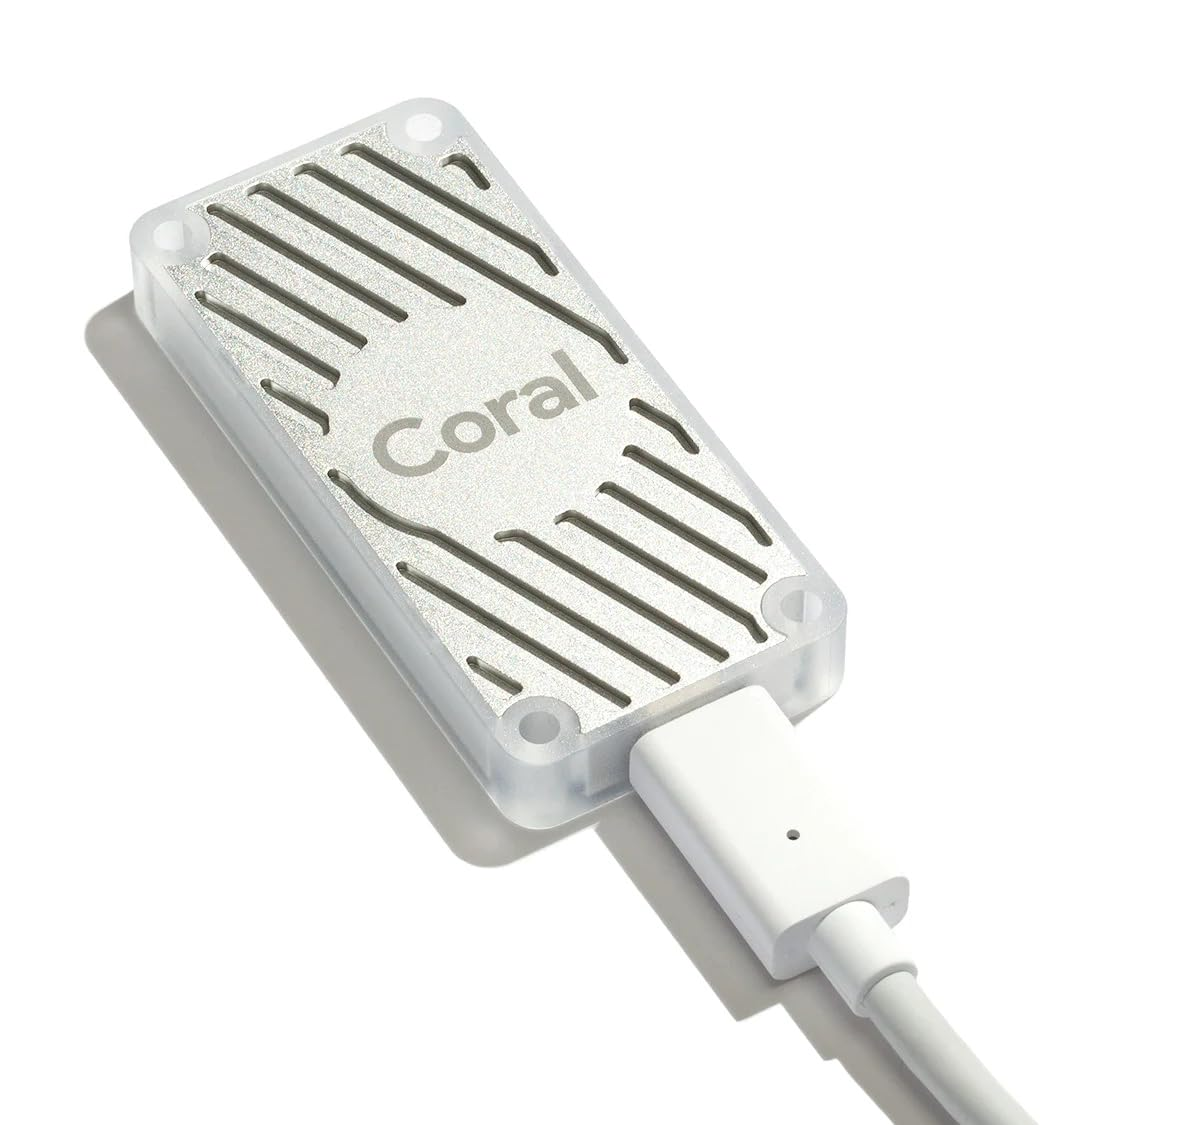
\includegraphics[height=4.3cm,trim=70 0 150 85,clip]{tpu_usb.jpg}\\[3pt]
        {\footnotesize (a) Coral USB Accelerator}
    \end{minipage}\hfill
    \begin{minipage}[b]{0.58\linewidth}
        \centering
        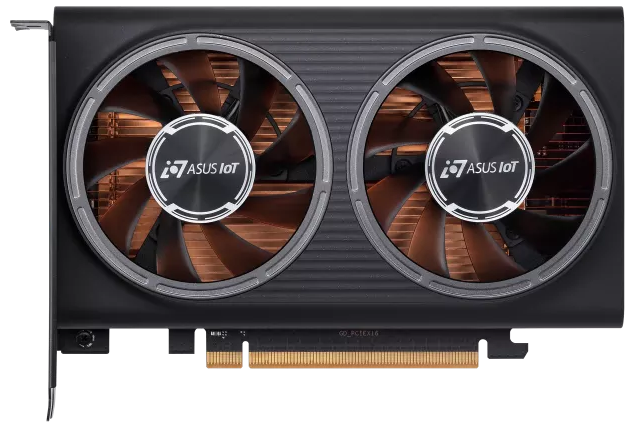
\includegraphics[height=4.3cm]{asus.png}\\[3pt]
        {\footnotesize (b) Carte ASUS CRL-G18U-P3DF}
    \end{minipage}
    \caption{Les deux supports employés dans ce stage, un Edge TPU au format USB pour l'axe mono-TPU et une carte PCIe qui en réunit 8 pour l'axe multi-TPU.}
    \label{fig:edgetpu}
\end{figure}

Malgré cette miniaturisation, les réseaux de neurones restent gourmands en mémoire et en énergie, ce qui pose la question de savoir comment exploiter au mieux les ressources disponibles d'un Edge TPU. C'est cette question qui a motivé le présent stage.

L'objectif était d'identifier les meilleurs compromis entre précision, latence et débit atteignables pour des réseaux de neurones exécutés sur Edge TPU, à travers deux axes complémentaires. Un axe mono-TPU, à orientation logicielle, a étudié l'effet de techniques de compression de modèles sur les performances. Un axe multi-TPU, à orientation matérielle, a étudié l'utilisation conjointe de plusieurs Edge TPU en pipeline ou en parallèle.

La suite est organisée comme suit. Le chapitre~\ref{chap:contexte} introduit le contexte, l'organisme d'accueil, le fonctionnement de l'Edge TPU et les contraintes qui en découlent. Le chapitre~\ref{chap:objectifs} précise les objectifs scientifiques du stage, les deux leviers d'optimisation qui en structurent les axes, et les livrables produits. Le chapitre~\ref{chap:methodo} décrit la méthodologie expérimentale et le framework de mesure, en traitant conjointement les configurations mono-TPU et multi-TPU. Le chapitre~\ref{chap:resultats} donne les résultats expérimentaux, en commençant par la validation du dispositif de mesure lui-même. Suivent les perspectives au chapitre~\ref{chap:perspectives} et la conclusion au chapitre~\ref{chap:conclusion}.


% =====================================================================
%  CHAPITRE 2 - CONTEXTE
% =====================================================================
\chapter{Contexte}
\label{chap:contexte}

\section{Laboratoire d'accueil et cadre du stage}

Le Laboratoire d'Analyse et d'Architecture des Systèmes (LAAS-CNRS) est une unité propre du Centre National de la Recherche Scientifique, située au 7 avenue du Colonel-Roche, 31031 Toulouse Cedex 4. Le laboratoire regroupe environ 700 personnes dans une vingtaine d'équipes de recherche, couvrant des domaines allant de la robotique à la micro-nanotechnologie. Les activités se caractérisent par une forte dimension expérimentale et une proximité avec l'industrie, notamment dans l'aéronautique, le spatial et les systèmes autonomes.

Le stage s'est déroulé au sein de l'équipe TRUST (Trustworthy systems: foundations and practices), rattachée au département RISC (Réseaux, Informatique et Systèmes de Confiance). L'équipe TRUST s'intéresse aux méthodes et outils permettant de justifier la confiance placée dans un système informatique : vérification pré-déploiement, surveillance à l'exécution, intelligence artificielle digne de confiance et frugale.

Le sujet s'inscrivait dans l'axe des systèmes embarqués temps-réel et des accélérateurs matériels pour l'IA. L'encadrant, Dr Tomasz Kłoda, travaille sur l'ordonnancement temps-réel de tâches d'inférence, en collaboration avec le LIRIS-CNRS à Lyon et la Technical University of Munich. La figure~\ref{fig:laas} montre l'entrée du laboratoire.

\begin{figure}[H]
    \centering
    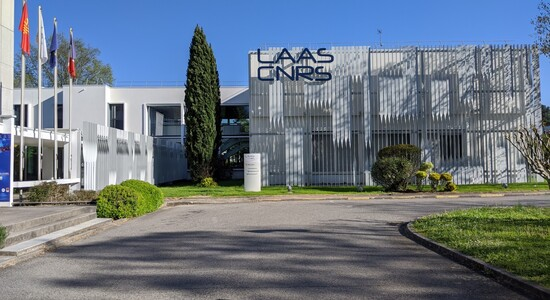
\includegraphics[width=0.75\linewidth]{LAAS.png}
    \caption{Entrée du LAAS-CNRS}
    \label{fig:laas}
\end{figure}

\section{Réseaux de neurones convolutifs en inférence}

Un réseau de neurones profond est une fonction paramétrée par des millions de coefficients appelés poids. Cette fonction se compose d'une succession de couches : chaque couche reçoit un tenseur de données d'entrée, applique une transformation linéaire (typiquement une multiplication matricielle ou une convolution) puis une fonction non-linéaire, et produit un tenseur de sortie qui alimente la couche suivante. L'apprentissage consiste à ajuster les poids sur la base d'un jeu de données étiquetées de manière à minimiser une erreur de prédiction. Une fois entraîné, le réseau est utilisé en inférence : on lui présente une donnée nouvelle (par exemple une image), il la propage à travers ses couches et produit un résultat (par exemple une classe d'objet).

L'inférence est l'opération que l'on cherche à accélérer dans les déploiements embarqués. À chaque exécution, le matériel doit récupérer les poids du modèle depuis la mémoire et effectuer la cascade d'opérations linéaires, qui se résument essentiellement à un très grand nombre de multiplications-accumulations. Ce sont précisément ces opérations qu'un TPU exécute en parallèle de manière optimisée.

Dans le cadre du stage, on s'est intéressé aux réseaux de neurones convolutifs (CNN), une famille d'architectures bien adaptée au traitement d'images. Les CNN exploitent le partage de paramètres pour détecter des motifs locaux (bords, textures puis structures de plus haut niveau) et constituent l'usage cible privilégié de l'Edge TPU. La figure~\ref{fig:cnn} en donne le schéma de principe.

\begin{figure}[H]
    \centering
    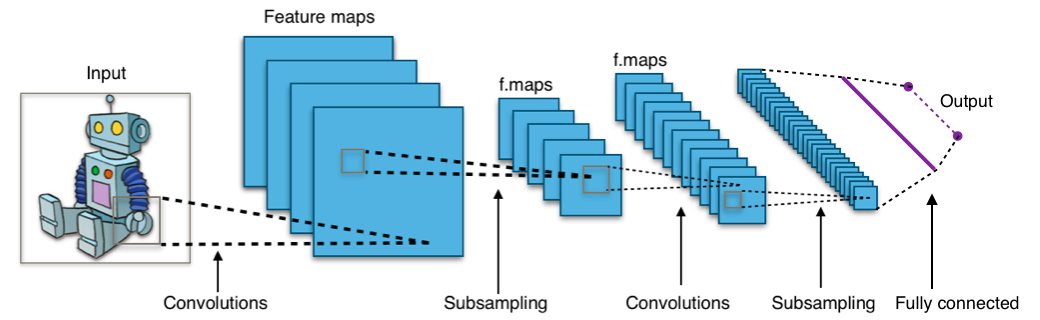
\includegraphics[width=0.75\linewidth]{conv.png}
    \caption{Schéma simplifié d'un CNN}
    \label{fig:cnn}
\end{figure}

\section{Architecture et exécution de l'Edge TPU}

L'Edge TPU est optimisé pour le déploiement embarqué : sa puissance théorique est de 4 TOPS, sa mémoire interne est limitée à 8 Mio de SRAM, et sa consommation maximale est de l'ordre de 2 W.

Cette miniaturisation s'accompagne de contraintes spécifiques. L'Edge TPU exécute uniquement des modèles quantifiés en INT8 (entiers signés sur 8 bits) et n'accélère qu'un sous-ensemble d'opérations : essentiellement les convolutions, les couches denses, les fonctions d'activation usuelles et certaines normalisations. Les opérations non supportées sont automatiquement repliées sur le processeur hôte par le compilateur Edge TPU, ce qui dégrade fortement les performances et limite de fait les architectures déployables.

Le principe de fonctionnement hardware d'un Edge TPU repose sur un réseau systolique (systolic array) \cite{kungWhySystolicArchitectures1982}. Une architecture systolique est un ensemble d'éléments de traitement (processing elements ou PE) interconnectés de manière régulière, où les données circulent de manière rythmée d'un élément au suivant, chaque élément effectuant une opération élémentaire avant de transmettre la donnée. Le principe, représenté sur la figure~\ref{fig:systolic}, est analogue à celui du pipeline dans les processeurs classiques, où plusieurs étages de traitement fonctionnent en parallèle sur des données différentes.

\begin{figure}[H]
    \centering
    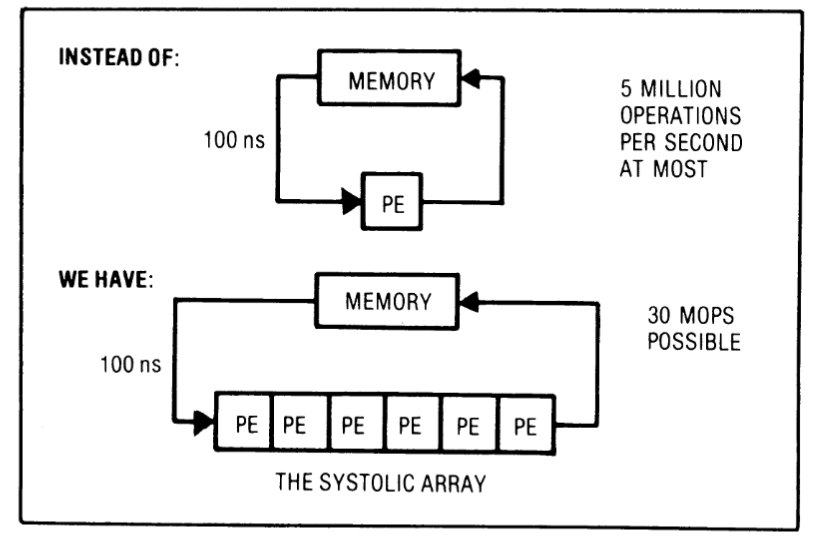
\includegraphics[width=0.5\linewidth]{systolic.png}
    \caption{Principe d'une architecture systolique}
    \label{fig:systolic}
\end{figure}

Dans le cas d'un réseau systolique destiné à la multiplication matricielle, ce principe est étendu à deux dimensions : les données circulent simultanément le long des lignes et des colonnes de la grille, ce qui permet d'atteindre un parallélisme très élevé avec un minimum d'accès mémoire. Les PE ici sont des unités de multiplication-accumulation (MAC) : chaque PE reçoit une donnée d'activation et un poids, les multiplie, ajoute le résultat à un accumulateur, et transmet la donnée à l'élément suivant.

L'exécution suit un mode SIMD (Single Instruction, Multiple Data) : la même opération s'applique à plusieurs paires (activation, poids) en parallèle dans chaque PE, qui dispose de plusieurs voies de calcul (compute lanes) \cite{seshadriEvaluationEdgeTPU2022}. C'est ce parallélisme massif à très bas niveau qui explique le rendement énergétique supérieur de l'Edge TPU pour les charges qu'il sait exécuter.

\section{Limites mémoire et performances}

Sur tout processeur, l'étage qui gère les accès mémoire est habituellement critique, tant en latence (l'étage mémoire conditionne souvent la fréquence d'horloge) qu'en consommation (les accès mémoire dominent la dissipation dynamique). Pour un accélérateur dont la charge de travail consiste à parcourir des millions de paramètres à chaque inférence, ces deux aspects sont particulièrement exacerbés.

Concrètement, lorsque le modèle dépasse la capacité de la SRAM interne de 8 Mio, les paramètres restants doivent être récupérés depuis la RAM hôte au fil de l'exécution. Ce phénomène, dit de streaming hors-puce (off-chip streaming), introduit un surcoût de latence significatif et fait souvent chuter les performances réelles bien en deçà des 4 TOPS théoriques.

% =====================================================================
%  CHAPITRE 3 - OBJECTIFS ET CONTRIBUTIONS
% =====================================================================
\chapter{Objectifs et contributions}
\label{chap:objectifs}

\section{Problématique}

Le stage visait à caractériser, pour des réseaux de neurones exécutés sur Edge TPU, les meilleurs compromis atteignables sur le triplet (latence, précision, débit). Pour un modèle donné, optimiser l'exécution sur Edge TPU revient à trouver un point d'équilibre entre trois grandeurs simultanément en jeu : la latence d'inférence (temps entre la présentation d'une donnée et la production du résultat), la précision (qualité des prédictions, mesurée par le pourcentage de classifications correctes sur un jeu de test) et le débit (nombre d'inférences traitées par seconde). Cette dernière grandeur ne se distingue de la latence que dans les configurations multi-TPU, où plusieurs accélérateurs traitent des inférences en parallèle ou en pipeline. Ces grandeurs sont en conflit. Comprimer un modèle réduit généralement la latence, au prix d'une dégradation de la précision. Il n'existe pas, en général, de configuration unique optimale sur tous les plans, mais un ensemble de configurations correspondant à différents compromis.

Ce compromis n'avait jamais été caractérisé sur cet accélérateur. La littérature de l'élagage structuré est abondante et compare ses critères entre eux sur des métriques logicielles, nombre de paramètres retirés ou nombre d'opérations économisées, c'est-à-dire sur des \emph{proxys} de la latence. Parallèlement, plusieurs travaux ont évalué les performances de l'Edge TPU \cite{seshadriEvaluationEdgeTPU2022,gaoWorkInProgressModeling2025,villarrubiaImprovingInferenceTime2023}, et établi que les transferts de poids depuis la mémoire hôte y dominent la latence. Mais à notre connaissance, aucun travail ne joint les deux : personne n'avait mesuré ce que ces critères d'élagage produisent réellement, en latence, sur un Edge TPU. Or rien ne garantit que le classement établi sur un proxy logiciel survive au passage sur un matériel dont la performance est gouvernée par un seuil de mémoire interne. C'est précisément ce point que l'étude visait à trancher par la mesure.

\section{Leviers d'optimisation et axes d'étude}

Le problème central est la mémoire. Deux familles de leviers complémentaires permettent de l'atténuer, et ont structuré les deux axes du stage.

Le levier logiciel consiste à comprimer le modèle pour réduire son empreinte mémoire. Si la compression est trop agressive, la précision du modèle se dégrade : il y a donc un compromis à explorer entre cette empreinte, dont la latence dépend sans lui être proportionnelle, et la qualité des prédictions. L'axe mono-TPU du stage lui a été consacré : il a caractérisé l'effet de plusieurs méthodes de compression sur les performances d'un modèle exécuté sur un seul Edge TPU, l'enjeu étant d'identifier quelles méthodes sont les plus pertinentes selon l'architecture du réseau et le régime mémoire observé.

Le levier matériel consiste à répartir le modèle sur plusieurs Edge TPU connectés en pipeline, chaque accélérateur ne gardant alors dans sa mémoire interne que les couches qu'il exécute. Les capacités s'additionnent, et un modèle trop volumineux pour un seul accélérateur peut ainsi tenir entièrement en mémoire interne. Ce même levier prend une seconde forme, l'emploi de plusieurs Edge TPU en parallèle, chacun traitant un échantillon différent. L'axe multi-TPU a étendu l'étude à ces topologies, ainsi qu'à leurs combinaisons. Chacune présente ses propres compromis entre latence, débit et capacité mémoire cumulée, et l'objet de cet axe était d'identifier les configurations dominantes selon le nombre d'accélérateurs disponibles.

Les deux leviers ne sont pas indépendants : la topologie matérielle retenue fixe la mémoire interne disponible par instance du modèle, donc le taux de compression nécessaire, donc la précision atteignable. C'est ce couplage qui a justifié de les traiter dans une méthodologie expérimentale unique, décrite au chapitre~\ref{chap:methodo}, où le fonctionnement détaillé de chaque topologie est présenté en section~\ref{sec:multitpu}.

\section{Livrables et retombées}

L'apport principal de ce stage est un ensemble d'analyses comparatives permettant d'orienter le choix d'une configuration de déploiement sur Edge TPU, obtenu à partir d'un framework développé au cours du stage.

\paragraph{Article de conférence.} La caractérisation de l'axe mono-TPU a fait l'objet d'un article, \emph{Pruning of Deep Neural Networks for Real-Time Execution on Edge TPU}, accepté à la conférence Digital System Design (DSD) et présenté à Cracovie le 2 septembre 2026.
Cet article couvre l'intégralité de l'axe mono-TPU du présent rapport : la chaîne de déploiement décrite en section~\ref{sec:conversion}, le protocole expérimental des sections~\ref{sec:modeles} et~\ref{sec:entrainement} et les résultats de la section~\ref{sec:res_mono}, auxquels le lecteur est renvoyé. S'y ajoute une seconde partie, en aval de cette caractérisation, qui exploite les profils (précision, temps d'exécution) mesurés pour sélectionner les taux d'élagage d'un ensemble de tâches périodiques ordonnancées sur un unique TPU, sous contrainte de respect des échéances. Cette partie relève des travaux d'ordonnancement temps-réel de l'équipe et n'est pas détaillée dans ce rapport ; elle illustre en revanche l'usage direct auquel les mesures produites ici sont destinées. Ma contribution personnelle a porté sur la totalité de la partie caractérisation : le framework, la campagne de mesure et son analyse.

\paragraph{Autres livrables.} S'y ajoutent : un framework de mesure automatisé couvrant la chaîne complète PyTorch $\rightarrow$ Edge TPU ; une campagne mono-TPU de 404 modèles élagués, sur une grille de 7 architectures, 7 critères d'importance et 9 taux d'élagage, entièrement caractérisés sur Edge TPU ; une campagne multi-TPU sur 8 architectures ImageNet-1k, 43 modèles mesurés dans les 22 manières de répartir les 8 accélérateurs de la carte ; et une étude complémentaire sur un corpus de 291 réseaux convolutifs synthétiques, servant d'une part à caractériser le comportement du pipeline en fonction de la résolution des entrées, d'autre part à identifier les sources d'interférence entre accélérateurs exécutés en parallèle.

% =====================================================================
%  CHAPITRE 4 - METHODOLOGIE
% =====================================================================
\chapter{Méthodologie et framework}
\label{chap:methodo}

\section{Architecture du framework}

L'objectif méthodologique était de produire, pour chaque modèle exploré, l'ensemble des configurations correspondant aux meilleurs compromis dans l'espace exploré, et d'analyser les facteurs qui les déterminent. L'outil de présentation principal est le front de Pareto sur les axes (latence, précision, débit), détaillé en section~\ref{sec:metriques}. On verra au chapitre~\ref{chap:resultats} que ce front se réduit souvent à un unique point de fonctionnement par modèle dans le plan (latence, débit), la configuration la plus rapide par échantillon étant alors également celle de plus haut débit ; ce n'est cependant vrai que lorsque le nombre d'accélérateurs nécessaires au modèle divise 8, et un arbitrage réapparaît sinon. L'identification de ces compromis dominants présentait par ailleurs un intérêt direct pour les travaux d'ordonnancement temps-réel menés par l'encadrant : connaître, pour chaque modèle, le jeu des configurations Pareto-optimales fournit un espace de choix qualifié dans lequel un ordonnanceur peut sélectionner le point de fonctionnement adapté à ses contraintes.

Le framework prend en entrée un modèle PyTorch et produit en sortie un ensemble de configurations comprimées caractérisées sur Edge TPU. Il a été conçu pour traiter de manière unifiée les configurations mono-TPU et les configurations multi-TPU, la topologie matérielle étant traitée comme une variable additionnelle des configurations explorées.

La suite du chapitre suit l'ordre dans lequel une configuration traverse ce framework. La section~\ref{sec:plateformes} décrit les plateformes matérielles sur lesquelles les mesures ont été relevées, et la section~\ref{sec:modeles} les deux panels de modèles et les jeux de données auxquels ils sont associés. La section~\ref{sec:pruning} décrit les méthodes de compression appliquées aux modèles, la section~\ref{sec:conversion} la chaîne de déploiement qui mène du modèle élagué au binaire exécutable sur l'accélérateur, et la section~\ref{sec:entrainement} le protocole d'entraînement et de récupération qui accompagne l'élagage. La section~\ref{sec:multitpu} décrit les manières d'employer plusieurs accélérateurs, la section~\ref{sec:metriques} les grandeurs mesurées et les représentations qui en ont été tirées, et la section~\ref{sec:conditions} le volume de calcul que l'ensemble a représenté.

\section{Plateformes matérielles}
\label{sec:plateformes}

Deux plateformes de mesure ont été utilisées, une par axe.

La première, dédiée à l'axe mono-TPU, est un Edge TPU au format USB (Coral USB Accelerator) connecté à une Raspberry Pi 4 Model B (ARM Cortex-A72) sous Raspberry Pi OS Lite. Cette plateforme est représentative d'un déploiement embarqué économique, et c'est le CPU de cette même carte qui sert de point de comparaison à toutes les mesures d'accélération rapportées au chapitre~\ref{chap:resultats}.

La seconde, dédiée à l'axe multi-TPU, est une carte PCIe CRL-G18U-P3DF \cite{AIAcceleratorPCIea} intégrant 8 Edge TPU sur un bus PCIe partagé, soit 64 Mio de mémoire interne cumulés. Ce sont ces 8 accélérateurs que les configurations décrites en section~\ref{sec:multitpu} répartissent, et le partage du bus entre eux est la principale source d'interférence à contrôler.

Ces deux plateformes ne servent qu'à l'inférence. Les entraînements et les phases de récupération ont été menés sur le cluster de calcul du LAAS, dont la configuration et le coût sont décrits en section~\ref{sec:conditions}.

\section{Panels de modèles et jeux de données}
\label{sec:modeles}

Chaque axe repose sur un panel de modèles et un jeu de données qui lui sont propres. Dans les deux cas, c'est le jeu de données qui a été fixé en premier et le panel d'architectures qui en découle.

\subsection{Modèles mono-TPU sur CIFAR-100}

Le jeu de données de l'axe mono-TPU est CIFAR-100 \cite{krizhevskyLearningMultipleLayers2009}, ensemble de 60 000 images de $32 \times 32$ pixels en RGB réparties en 100 classes, dont 50 000 pour l'entraînement et 10 000 pour le test. Deux raisons ont présidé à ce choix. La première est le coût : bien qu'éloigné d'un cas industriel, CIFAR-100 est suffisamment petit pour permettre l'exploration d'un grand nombre de configurations en un temps raisonnable, ce que la comparaison systématique de 7 critères d'importance exigeait. La seconde est la comparabilité : CIFAR-100 est la référence de la littérature du pruning structuré, la grande majorité des travaux du domaine y reportant leurs résultats, ce qui permet de situer les nôtres par rapport à l'état de l'art.

\begin{figure}[H]
    \centering
    
\includegraphics[width=0.5\linewidth]{cifar100.png}
    \caption{Exemples d'images du dataset CIFAR-100 avec leurs étiquettes de classe}
    \label{fig:cifar100}
\end{figure}

Le choix des architectures découle de celui du jeu de données : les 7 retenues sont celles que cette même littérature emploie, ce qui préserve la comparabilité avec les travaux existants. Elles couvrent par ailleurs un éventail représentatif d'architectures déployables sur Edge TPU :

\begin{itemize}
  \item ResNet-18 (11 M paramètres) et ResNet-50 (24 M paramètres). Architectures à connexions résiduelles, références incontournables en classification d'images.
  \item VGG-19 (20 M paramètres). Architecture monolithique sans skip connections, représentative des designs anciens dominés par les couches convolutives empilées.
  \item WRN-28-10 (37 M paramètres). Wide Residual Network, version élargie des ResNet, choisi pour tester un régime fortement contraint en mémoire.
  \item MobileNetV2 (2,4 M paramètres). Architecture conçue pour le mobile à l'aide de convolutions séparables en profondeur, représentative des designs compacts.
  \item GoogLeNet (5,7 M paramètres). Architecture à branches parallèles (modules Inception), représentative de topologies non linéaires.
  \item SqueezeNet 1.1 (0,8 M paramètres). Architecture très compacte, choisie comme cas limite pour les très petits modèles sans BatchNorm.
\end{itemize}

Ces architectures sont employées dans leurs variantes adaptées à la petite taille des images de CIFAR-100. Conçues à l'origine pour des images bien plus grandes, elles en réduisent les dimensions dès les premières couches, ce qui ne laisserait presque rien à traiter à partir d'une entrée de $32 \times 32$ pixels ; leurs premiers étages ont donc été ajustés, adaptation standard du domaine.

\subsection{Modèles multi-TPU sur ImageNet-1k}

L'axe multi-TPU a changé de jeu de données comme de panel. Le jeu retenu est ImageNet-1k \cite{dengImageNetLargeScaleHierarchical2009}, ensemble de 1,28 million d'images d'entraînement réparties en 1000 classes, avec un ensemble de validation de 50 000 images, dont la figure~\ref{fig:imagenet} donne quelques exemples.

\begin{figure}[H]
    \centering
    
\includegraphics[width=\linewidth]{imagenet.png}
    \caption{Exemples d'images du jeu de données ImageNet-1k. À comparer aux images de $32 \times 32$ pixels de la figure~\ref{fig:cifar100} : c'est ce changement d'échelle qui rend la capacité des modèles réellement sollicitée, et donc le coût de la compression mesurable.}
    \label{fig:imagenet}
\end{figure}

Ce basculement tient à la différence d'objectif entre les deux axes. Le premier compare des critères d'élagage entre eux, et c'est leur classement relatif qui porte la conclusion, davantage que la valeur absolue de la précision. Le second pose une tout autre question, celle de la répartition des accélérateurs, et ne mobilise qu'un critère unique : la précision n'y intervient plus que comme une valeur par configuration, mise en regard du gain de performance obtenu, sans autre lecture pour la corroborer. Elle doit donc être de bonne qualité en elle-même, ce que CIFAR-100 ne permet pas : sa faible résolution et son faible nombre de classes rendent les modèles fortement sur-paramétrés pour la tâche, si bien qu'un élagage même sévère y dégrade peu la précision. Il fallait un jeu de données où la capacité du modèle est réellement sollicitée pour que le prix de la compression devienne mesurable, ce qui permet du même coup de confronter les conclusions de l'axe mono-TPU à un régime où l'élagage coûte.

Le prix à payer est le coût de calcul : une époque d'entraînement passe d'environ 40 secondes sur CIFAR-100 à 20 minutes à 2 heures sur ImageNet-1k selon l'architecture et la résolution, soit un facteur 30 à 180. Cette différence explique que l'axe mono-TPU explore une grille complète de critères et de taux, tandis que le second se restreint à un critère unique et à quelques taux ciblés.

Le panel a changé pour deux raisons. La première est une nécessité de taille : la question du partitionnement sur plusieurs accélérateurs ne se pose que pour des modèles suffisamment gros pour justifier de cumuler leurs mémoires internes, or le panel CIFAR-100 se concentre dans le bas de cette échelle, son plus gros modèle occupant 35 Mio quand 8 accélérateurs en cumulent 64. La seconde tient au choix de ces 8 architectures en particulier : ce sont celles retenues par des travaux d'ordonnancement sur Edge TPU pipelinés menés par l'encadrant du stage et un doctorant \cite{sunSAParSurrogateAssisted2025}, et reprendre leur panel rend les mesures produites ici directement exploitables par ces travaux.

Les 8 architectures sont employées dans leur résolution native ($224 \times 224$ ou $299 \times 299$ pixels) et à partir de poids ImageNet-1k pré-entraînés publics. Leurs tailles après quantification INT8 sont données ci-dessous : ce sont celles des fichiers TFLite produits par la chaîne de conversion décrite en section~\ref{sec:conversion}, exprimées en mébioctets, de manière à être directement comparables au plafond de 8 Mio de la mémoire interne et aux volumes que rapporte le compilateur Edge TPU, qui emploie la même unité.

\begin{itemize}
  \item GoogLeNet (6,57 Mio), BN-Inception (11,08 Mio), Inception-V3 (23,24 Mio) et Inception-V4 (41,60 Mio). Quatre générations successives de la famille Inception, construite sur des modules à branches parallèles.
  \item Inception-ResNet-V2 (55,36 Mio). Hybride combinant les branches parallèles de la famille Inception et les connexions résiduelles.
  \item ResNet-50 (25,09 Mio), ResNet-101 (43,88 Mio) et ResNet-152 (59,39 Mio). Trois profondeurs croissantes de la famille résiduelle.
\end{itemize}

Le panel couvre donc un rapport de 9 entre le plus petit et le plus gros modèle, et seul GoogLeNet approche les 8 Mio d'un unique Edge TPU, sans toutefois y tenir tout à fait, comme le montrera le chapitre~\ref{chap:resultats}. Les deux familles sont représentées à taille comparable (ResNet-101 et Inception-V4 d'une part, ResNet-152 et Inception-ResNet-V2 d'autre part), ce qui permet de comparer résiduels et branches parallèles à nombre de paramètres apparié.

\subsection{Protocoles d'évaluation de la précision}

Sur l'axe mono-TPU, la précision INT8 a été mesurée sur l'intégralité des 10 000 images de test de CIFAR-100, dont la taille modeste rend l'évaluation complète sur accélérateur abordable pour les 404 configurations du panel.

Sur l'axe multi-TPU, deux protocoles coexistent. La précision en flottant a été mesurée sur les 50 000 images de validation à chaque époque de récupération, ce qui sert de signal de suivi de l'entraînement. La précision INT8 effectivement obtenue sur l'accélérateur a été mesurée séparément sur un sous-ensemble de 5000 images de validation, l'évaluation complète sur Edge TPU étant prohibitive en temps sur les configurations comparées. Ce sous-ensemble est le même pour toutes les configurations, tiré une fois pour toutes, ce qui rend les précisions de l'axe multi-TPU directement comparables entre elles ; les écarts inférieurs à quelques dixièmes de point y restent néanmoins à la limite de ce que 5000 images permettent de trancher. Seule cette seconde mesure décrit ce que fait le modèle déployé ; les deux séries de chiffres ne sont pas directement comparables et sont présentées comme telles au chapitre~\ref{chap:resultats}.



\section{Méthodes de compression et de pruning}
\label{sec:pruning}

Deux méthodes de compression ont été utilisées, l'une obligatoire et l'autre facultative.

La quantification est l'opération qui réduit la précision numérique des poids et activations d'un format flottant 32 bits vers un format entier de plus faible largeur. Sur Edge TPU, la quantification INT8 est obligatoire : le matériel ne sait pas exécuter des modèles flottants. Elle consiste, brièvement, à observer la distribution des activations sur un petit échantillon représentatif des données (calibration), à en déduire des facteurs d'échelle par tenseur, puis à arrondir les poids et les activations à des entiers signés sur 8 bits. La dégradation de précision induite par cette opération est généralement faible (de l'ordre de 1 à 3 points de pourcentage de précision Top-1 sur un dataset comme CIFAR-100), au bénéfice d'une division par 4 de la taille mémoire des paramètres.

Le pruning structuré est la méthode centrale de l'étude. Il consiste à supprimer définitivement des groupes entiers de paramètres dans le réseau (canaux entiers d'une convolution, neurones d'une couche dense) jugés peu importants. Contrairement au pruning non structuré, qui se contente d'annuler des poids individuels (et reste sans effet sur la latence côté Edge TPU, qui ne sait pas exploiter cette sparsité), le pruning structuré réduit physiquement la taille du modèle et donc le nombre d'opérations à exécuter et la mémoire à transférer.

La principale difficulté pratique du pruning structuré est le suivi des dépendances : supprimer un filtre dans une couche convolutive implique de propager la suppression sur toutes les couches connectées. Cette tâche a été confiée à la bibliothèque torch\_pruning, qui implémente un algorithme de Dependency Graph \cite{fangDepGraphAnyStructural2023} automatisant ces propagations. La figure~\ref{fig:depgraph} donne les types de dépendances qu'il doit résoudre.

\begin{figure}[H]
    \centering
    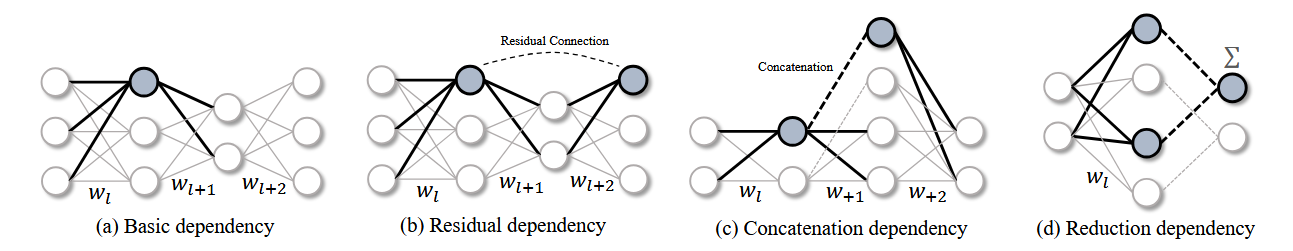
\includegraphics[width=1\linewidth]{dependence.png}
    \caption{Types de dépendances dans les architectures CNN conventionnelles}
    \label{fig:depgraph}
\end{figure}

Une fois la machinerie de pruning structuré disponible, la question centrale est : quels filtres supprimer ? On choisit en pratique un score d'importance, on classe les filtres par score, et on supprime ceux du bas. La littérature propose de nombreux scores d'importance ; en suivant le panorama dressé par le survey de He et Xiao \cite{heStructuredPruningDeep2024} sur le pruning structuré des réseaux convolutifs profonds, on en distingue traditionnellement deux familles selon la nature des informations qu'ils consomment.

\paragraph{Critères data-free.} Ils n'utilisent que les poids appris du modèle pour estimer l'importance, sans recours aux données d'apprentissage. Ils sont les moins coûteux à évaluer, puisqu'aucune passe d'inférence n'est nécessaire. Les critères retenus sont les suivants :

\begin{itemize}
  \item \textbf{Magnitude L1} : norme L1 des poids du filtre. L'hypothèse sous-jacente, la plus ancienne du domaine, est qu'un filtre de faible amplitude contribue peu à la sortie et peut être retiré sans dommage.
  \item \textbf{Magnitude L2} : même hypothèse, avec une norme euclidienne, qui pénalise davantage les poids isolés de forte amplitude qu'une distribution uniforme de même somme.
  \item \textbf{FPGM} (Filter Pruning via Geometric Median) : plutôt que de supprimer les filtres de faible norme, ce critère supprime les filtres les plus proches de la médiane géométrique des filtres de leur couche, c'est-à-dire les plus redondants. Un filtre de forte norme mais quasi identique à ses voisins est donc éliminé, ce que les critères de magnitude conservent.
  \item \textbf{Random} : sélection aléatoire des filtres. Ce n'est pas une méthode mais la référence de contrôle indispensable : tout critère qui ne bat pas significativement le hasard après récupération n'apporte rien.
\end{itemize}

\paragraph{Critères data-driven.} Ils exploitent les données d'entraînement, sous des formes qui n'ont pas le même effet et qu'il faut donc distinguer d'emblée. Cette dépendance prend en effet deux visages, dont on verra au chapitre~\ref{chap:resultats} qu'ils ne se valent pas. Les deux premiers critères l'exercent au moment de l'élagage, par des passes avant et arrière sur un lot de calibration avant chaque étape ; le troisième la reporte entièrement en amont, dans une phase d'entraînement préalable, et n'exploite ensuite que les poids du modèle. Les critères retenus sont les suivants :

\begin{itemize}
  \item \textbf{Taylor} : produit du poids par son gradient, qui constitue une approximation au premier ordre de la variation de la fonction de coût induite par la mise à zéro du filtre. Ce critère estime donc directement ce que l'on cherche à minimiser, au lieu de s'appuyer sur un indicateur indirect comme la norme.
  \item \textbf{OBD-C} : approximation au second ordre de la même variation. Le calcul de la hessienne complète étant hors de portée, OBD-C l'approche par une matrice d'information de Fisher factorisée par couche, ce qui est plus fidèle que l'approximation diagonale classique d'Optimal Brain Damage. Plus informé que Taylor en théorie, mais nettement plus fragile en pratique : son implémentation échoue sur les convolutions séparables en profondeur de MobileNetV2, sur les modules Fire de SqueezeNet et sur VGG-19.
  \item \textbf{BN-Scale} : amplitude des paramètres $\gamma$ de la couche de normalisation par lot qui suit la convolution. Comme $\gamma$ multiplie directement le canal de sortie, un $\gamma$ proche de zéro annule le canal. Sa dépendance aux données ne vient pas d'une estimation par gradient au moment de l'élagage, mais d'une phase préalable d'apprentissage de la parcimonie, où une régularisation L1 sur les $\gamma$ pousse ceux des canaux inutiles vers zéro et rend le classement discriminant ; cette phase coûte un entraînement complet supplémentaire par modèle. C'est donc le critère le plus coûteux du panel, mais son coût est payé en amont et non à chaque étape d'élagage. Il est inapplicable à SqueezeNet, qui ne comporte pas de normalisation par lot.
\end{itemize}

Sept critères ont donc été évalués au total sur les 7 architectures de l'axe mono-TPU, et le produit cartésien complet compte $7 \times 7 \times 9 = 441$ configurations. Il en manque 37, pour deux raisons distinctes. Parmi elles, 36 sont des incompatibilités structurelles, systématiques sur les 9 taux d'élagage : BN-Scale est indisponible sur SqueezeNet (9 configurations) et OBD-C sur VGG-19, MobileNetV2 et SqueezeNet (27 configurations). La trente-septième est un échec isolé et d'une autre nature : la configuration WRN-28-10 $\times$ BN-Scale à 20~\% a bien été élaguée et récupérée, mais a échoué à la quantification INT8 de la chaîne décrite en section~\ref{sec:conversion}, le quantificateur ne parvenant pas à retrouver les tenseurs du sous-graphe converti. Faute de temps de calcul, elle n'a pas été rejouée. Les classements présentés au chapitre~\ref{chap:resultats} sont normalisés en conséquence, de manière à ce qu'une indisponibilité ne fausse pas le rang des critères disponibles.

\paragraph{Restriction pour l'axe multi-TPU.} La comparaison des 7 critères n'a été menée que sur l'axe mono-TPU. L'axe multi-TPU n'a mobilisé qu'un seul critère, Taylor, retenu parmi les mieux classés de la campagne mono-TPU. Ce choix a été imposé par le coût d'une configuration, sans commune mesure entre les deux axes, ce que détaille la section~\ref{sec:conditions} : y répliquer la grille complète des critères était hors d'atteinte. La portée qu'en perdent les conclusions comparatives est discutée au chapitre~\ref{chap:perspectives}.

\section{Conversion et déploiement des modèles}
\label{sec:conversion}

L'élagage décrit ci-dessus opère sous PyTorch, alors que l'Edge TPU n'exécute que des modèles TFLite quantifiés en INT8. Faire passer les modèles de l'un à l'autre a constitué la principale difficulté d'ingénierie du stage.

La chaîne complète de déploiement comprend les étapes suivantes : entraînement PyTorch, export ONNX, conversion TFLite float32, quantification INT8, puis compilation Edge TPU. La bibliothèque torch\_pruning n'existe qu'en PyTorch. L'Edge TPU n'accepte en revanche que des modèles TFLite issus de TensorFlow. Les deux frameworks décrivent les graphes de calcul de manière différente et ne supportent pas exactement les mêmes opérations, ce qui rend la conversion non triviale. La solution adoptée s'appuie sur le format intermédiaire ONNX : le modèle élagué en PyTorch est exporté en ONNX, converti en TensorFlow par les outils onnx2tf, quantifié par ai-edge-quantizer puis compilé pour l'Edge TPU. La figure~\ref{fig:chaine} résume cet enchaînement et l'outil responsable de chaque transition.

\begin{figure}[H]
\centering
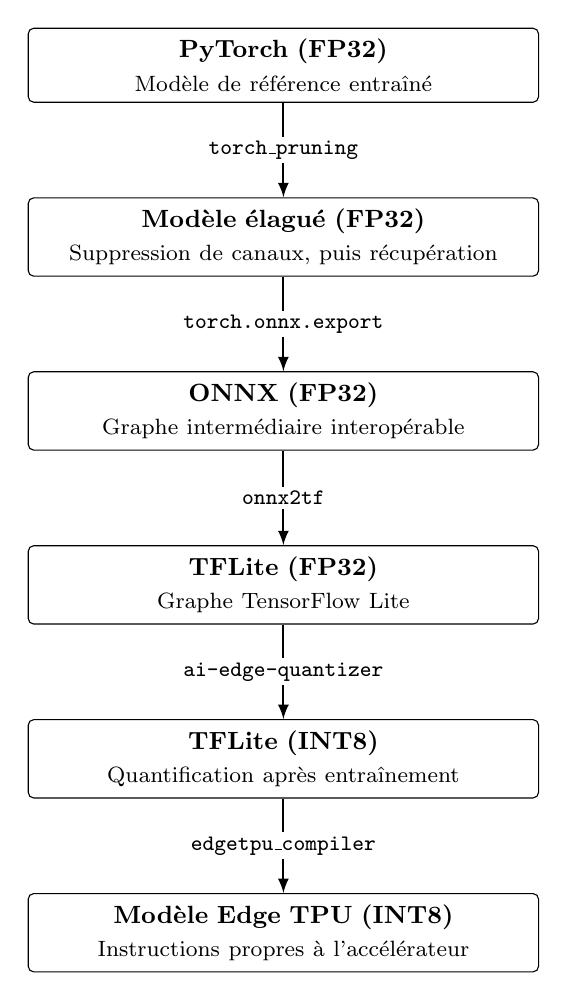
\begin{tikzpicture}[
  node distance = 12mm,
  etape/.style  = {draw, rounded corners=2pt, align=center,
                   text width=62mm, inner sep=4pt, font=\small},
  fleche/.style = {-latex, thick},
  outil/.style  = {font=\footnotesize\ttfamily, midway, fill=white, inner sep=1.5pt}
]
\node[etape] (a) {\textbf{PyTorch (FP32)}\\[1pt]\footnotesize Modèle de référence entraîné};
\node[etape, below=of a] (b) {\textbf{Modèle élagué (FP32)}\\[1pt]\footnotesize Suppression de canaux, puis récupération};
\node[etape, below=of b] (c) {\textbf{ONNX (FP32)}\\[1pt]\footnotesize Graphe intermédiaire interopérable};
\node[etape, below=of c] (d) {\textbf{TFLite (FP32)}\\[1pt]\footnotesize Graphe TensorFlow Lite};
\node[etape, below=of d] (e) {\textbf{TFLite (INT8)}\\[1pt]\footnotesize Quantification après entraînement};
\node[etape, below=of e] (f) {\textbf{Modèle Edge TPU (INT8)}\\[1pt]\footnotesize Instructions propres à l'accélérateur};
\draw[fleche] (a) -- node[outil] {torch\_pruning}      (b);
\draw[fleche] (b) -- node[outil] {torch.onnx.export}   (c);
\draw[fleche] (c) -- node[outil] {onnx2tf}             (d);
\draw[fleche] (d) -- node[outil] {ai-edge-quantizer}   (e);
\draw[fleche] (e) -- node[outil] {edgetpu\_compiler}   (f);
\end{tikzpicture}
\caption[Chaîne de déploiement PyTorch vers Edge TPU]{Chaîne de déploiement complète, du modèle PyTorch entraîné au modèle exécutable sur Edge TPU. L'outil responsable de chaque transition est indiqué sur la flèche correspondante.}
\label{fig:chaine}
\end{figure}

Deux correctifs ont dû être appliqués aux bibliothèques amont pour que les panels de la section~\ref{sec:modeles} traversent la chaîne au complet : un correctif de la conversion de l'opérateur de remplissage dans onnx2tf et un correctif de la validation des rangs de tenseurs dans ai-edge-quantizer, sans lesquels GoogLeNet et SqueezeNet, présents l'un et l'autre dans le panel de l'axe mono-TPU, sont rejetés par le compilateur Edge TPU. Par ailleurs, le compilateur ne segmente correctement que les fichiers TFLite issus de certains chemins de conversion : les modèles produits par le convertisseur TensorFlow natif provoquent une faute de segmentation du compilateur dès que l'on demande plus d'un segment, alors que les mêmes modèles produits via le chemin ONNX se compilent normalement. Ce point a conditionné toute la campagne multi-TPU.

Il faut en tirer une réserve sur la portée du framework. La chaîne repose sur un empilement d'outils en évolution rapide, dont plusieurs sont ici employés en dehors du cadre pour lequel ils sont maintenus, et dont l'assemblage n'est stable que pour un jeu de versions donné : les correctifs décrits ci-dessus visent l'état actuel de ces bibliothèques et n'ont aucune raison de rester valables sur leurs versions ultérieures, où ils pourront aussi bien devenir inutiles que cesser de s'appliquer. Le framework ne garantit donc pas de convertir une architecture arbitraire : la garantie ne porte que sur les modèles effectivement convertis pour cette étude, dont chacun a été validé individuellement. Toute architecture nouvelle doit être considérée comme non supportée tant qu'elle n'a pas traversé la chaîne complète et passé les contrôles de la section~\ref{sec:validation}. Cette contrainte a d'ailleurs pesé sur la constitution des deux panels décrits plus haut, plusieurs candidats ayant dû être écartés faute de traverser la chaîne.

\section{Protocole d'entraînement et de récupération}
\label{sec:entrainement}

Les réglages d'entraînement n'agissent pas indépendamment les uns des autres, et une mauvaise configuration conduit à des modèles non convergés ou sur-appris, deux situations qui invalident les comparaisons ultérieures. Comme chaque essai coûte un entraînement complet, les explorer était hors de portée. L'axe mono-TPU a donc repris telle quelle la recette du papier PruningBench \cite{liComprehensiveStudyStructural2025}, protocole uniforme appliqué à un large panel de méthodes de pruning sur classification CIFAR : taux d'apprentissage et sa planification, taille des lots, nombre d'époques, optimiseur et coefficient de régularisation en sont issus sans modification. Cette uniformité présente deux avantages : elle isole la variable d'intérêt, le choix du critère d'importance, en figeant toutes les autres, et elle permet de positionner les résultats du stage par rapport au leaderboard publié de PruningBench.

Le protocole s'est déroulé en trois temps. Chaque modèle de référence a d'abord été entraîné depuis zéro pendant 200 époques. Il a ensuite été élagué progressivement, en de nombreuses étapes successives plutôt qu'en une seule fois, ce qui laisse le réseau s'ajuster au fur et à mesure ; la sélection des filtres à retirer a été faite sur l'ensemble du réseau plutôt que couche par couche, de sorte que l'algorithme répartit lui-même l'élagage entre les couches, et une même couche ne pouvait jamais être vidée au-delà de 90 \% de ses paramètres, faute de quoi le réseau serait coupé en deux. Est venue enfin une phase de récupération de 100 époques, qui reprend les réglages de l'entraînement initial avec un taux d'apprentissage 10 fois plus faible : il ne s'agit plus d'apprendre la tâche, mais de réparer ce que l'élagage a détruit.

Un écart au protocole PruningBench mérite d'être signalé, car il conditionne la comparabilité des résultats. PruningBench définit sa cible d'élagage comme un pourcentage de réduction du nombre d'opérations de multiplication-accumulation ; elle a été définie ici comme un pourcentage de paramètres retirés. Ce choix est dicté par l'objet de l'étude : sur Edge TPU, c'est l'empreinte mémoire, donc le nombre de paramètres, qui détermine si le modèle tient en SRAM et donc la latence. Les tableaux chiffrés ne sont en conséquence pas directement superposables à ceux de PruningBench, et le classement de certains critères peut se déplacer entre les deux formulations, puisque certains critères élaguent préférentiellement des paramètres à fort coût de calcul unitaire. Les tendances qualitatives restent transférables.

\paragraph{Protocole multi-TPU.} La recette PruningBench n'était pas transposable à ImageNet-1k : elle suppose un entraînement de référence depuis zéro, dont le coût aurait été ici de plusieurs milliers d'heures de calcul. L'axe multi-TPU est donc parti de poids pré-entraînés publics, déjà disponibles pour ces architectures, et s'est limité à la phase de récupération, pour laquelle il a repris les réglages usuels de la littérature de l'élagage sur ImageNet. L'algorithme d'élagage est celui de l'axe mono-TPU, avec le seul critère Taylor, et une seule différence : le plafond par couche a été relevé de 90 à 95 \%, sans quoi les taux les plus sévères étaient hors d'atteinte.

Ces réglages sont identiques d'un modèle à l'autre. Le seul degré de liberté est le budget de récupération, c'est-à-dire le nombre d'époques, fixé en fonction du taux d'élagage effectivement atteint : de 15 époques en dessous de 10 \% de paramètres retirés à 90 au-delà de 85 \%. Ce couplage est nécessaire et non arbitraire : un modèle élagué à 90 \% voit sa précision retomber au niveau du hasard immédiatement après l'élagage et demande un budget de récupération sans commune mesure avec un modèle élagué à 25 \%, qui conserve l'essentiel de sa précision. Attribuer le même budget aux deux aurait introduit un biais systématique en faveur des taux faibles.

Ce point a d'ailleurs fait l'objet d'un correctif en cours de campagne. Le budget était initialement décidé à partir du taux d'élagage \emph{prédit} par un modèle de premier ordre assimilant un paramètre à un octet ; or ce modèle sous-estime systématiquement l'occupation réelle de la SRAM, qui inclut les activations intermédiaires et les grandeurs internes des couches de normalisation, et l'élagage réellement nécessaire s'est révélé plus profond de 6 à 35 points selon le modèle. Le budget a donc été décidé, dans la suite de la campagne, après l'élagage, à partir du taux effectivement atteint.

\section{Configurations multi-TPU}
\label{sec:multitpu}

Lorsque plusieurs Edge TPU sont disponibles sur une même plateforme, il n'existe que deux leviers élémentaires pour les employer, dont toutes les configurations réalisables sont des combinaisons.

\subsection{Pipeline}

Le modèle est partitionné le long de ses couches \cite{villarrubiaImprovingInferenceTime2023} : chaque TPU exécute une portion contiguë du réseau et transmet son activation de sortie au TPU suivant. L'intérêt décisif de ce levier est que les SRAM des TPU s'additionnent : un modèle trop gros pour un seul accélérateur, et donc condamné au streaming hors-puce, peut tenir entièrement en mémoire interne une fois réparti sur plusieurs. Son inconvénient est double. D'une part la latence d'une inférence individuelle augmente, puisque l'échantillon doit traverser tous les étages et franchir autant de frontières de partition. D'autre part la carte n'offre aucun lien direct de TPU à TPU : le transfert de l'activation d'un étage vers le suivant transite par la RAM hôte via le bus PCIe, et chaque frontière de partition a donc un coût propre, mesuré dans nos expériences entre 0,2 et 2,8 ms par segment selon le volume de l'activation transmise. Le débit, en revanche, augmente : les étages travaillent simultanément sur des échantillons différents.

Le partitionnement opère à la granularité de la couche entière : la SRAM d'un Edge TPU ne peut accueillir que des couches complètes, et non une fraction de couche. Une portion de pipeline est donc un bloc de couches consécutives, et la coupure ne peut tomber qu'à une frontière de couche. Cette contrainte rend le partitionnement des architectures non séquentielles non trivial : un module Inception de GoogLeNet ou un bloc résiduel de ResNet n'est pas une simple pile linéaire de couches. Le découpage a été entièrement délégué au compilateur Edge TPU, qui décide seul du placement des coupures ; la seule prise dont on disposait est le nombre de segments demandés. Les limites que cette délégation impose sont discutées au chapitre~\ref{chap:perspectives}.

\subsection{Parallélisme}

Chaque TPU exécute des inférences indépendantes sur des échantillons différents. La latence individuelle est strictement inchangée, et le débit cumulé croît proportionnellement au nombre d'accélérateurs. Ce levier ne présente donc aucun inconvénient intrinsèque, mais il ne résout pas le problème de la mémoire : chaque copie doit tenir seule dans les 8 Mio d'un TPU, sans quoi chacune paie le streaming hors-puce. Il reste la question des interférences sur le bus PCIe partagé entre les 8 accélérateurs, que la campagne quantifie explicitement.

\subsection{Configurations hybrides}

À 8 accélérateurs disponibles, les deux leviers se composent. Une répartition consiste à découper les 8 accélérateurs en instances, chacune exécutant le modèle sur autant d'étages qu'elle compte d'accélérateurs ; il en existe exactement 22, autant que de façons d'écrire 8 comme une somme d'entiers. Quatre d'entre elles sont homogènes, toutes leurs instances ayant la même profondeur, et ce sont les seules disponibles lorsque le nombre d'accélérateurs nécessaires à une instance divise 8 : 8 copies indépendantes, 4 pipelines de 2, 2 pipelines de 4, ou un unique pipeline de 8. La figure~\ref{fig:configs} les représente.

\begin{figure}[H]
\centering
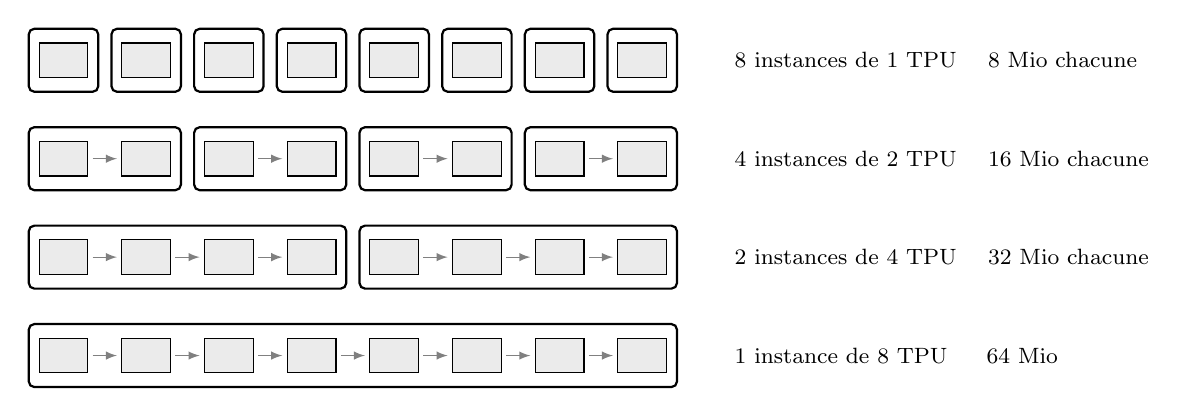
\begin{tikzpicture}[x=1.05cm, y=1.25cm,
  tpu/.style  = {draw, fill=black!8, minimum width=0.62cm, minimum height=0.44cm,
                 inner sep=0pt, font=\tiny},
  grp/.style  = {draw, thick, rounded corners=2pt},
  flx/.style  = {-latex, gray, shorten >=1pt, shorten <=1pt},
  lgd/.style  = {font=\footnotesize, anchor=west}
]
% --- ligne 1 : 8 instances de 1 TPU ---
\foreach \i in {0,...,7} { \node[tpu] at (\i,0) {}; }
\foreach \i in {0,...,7} { \draw[grp] (\i-0.42,-0.32) rectangle (\i+0.42,0.32); }
\node[lgd] at (8.0,0) {8 instances de 1 TPU \quad 8 Mio chacune};

% --- ligne 2 : 4 pipelines de 2 TPU ---
\foreach \i in {0,...,7} { \node[tpu] at (\i,-1) {}; }
\foreach \s in {0,2,4,6} {
  \draw[grp] (\s-0.42,-1.32) rectangle (\s+1.42,-0.68);
  \draw[flx] (\s+0.32,-1) -- (\s+0.68,-1);
}
\node[lgd] at (8.0,-1) {4 instances de 2 TPU \quad 16 Mio chacune};

% --- ligne 3 : 2 pipelines de 4 TPU ---
\foreach \i in {0,...,7} { \node[tpu] at (\i,-2) {}; }
\foreach \s in {0,4} { \draw[grp] (\s-0.42,-2.32) rectangle (\s+3.42,-1.68); }
\foreach \i in {0,1,2,4,5,6} { \draw[flx] (\i+0.32,-2) -- (\i+0.68,-2); }
\node[lgd] at (8.0,-2) {2 instances de 4 TPU \quad 32 Mio chacune};

% --- ligne 4 : 1 pipeline de 8 TPU ---
\foreach \i in {0,...,7} { \node[tpu] at (\i,-3) {}; }
\draw[grp] (-0.42,-3.32) rectangle (7.42,-2.68);
\foreach \i in {0,...,6} { \draw[flx] (\i+0.32,-3) -- (\i+0.68,-3); }
\node[lgd] at (8.0,-3) {1 instance de 8 TPU \quad\ 64 Mio};
\end{tikzpicture}
\caption[Les 4 répartitions homogènes de 8 accélérateurs]{Les 4 manières homogènes de répartir les 8 Edge TPU de la carte, sur les 22 possibles. Chaque rectangle est un accélérateur, chaque encadré une instance du modèle, et les flèches marquent le passage de l'activation d'un étage au suivant.}
\label{fig:configs}
\end{figure}

Ces 4 configurations mobilisent exactement les mêmes ressources matérielles et ne diffèrent que par la manière de les organiser. Avec les 18 répartitions hétérogènes, elles constituent l'espace de comparaison de l'axe multi-TPU. Chacune impose au modèle une contrainte de taille différente, puisque la SRAM disponible par instance est de 8, 16, 32 ou 64 Mio respectivement, et donc un taux d'élagage différent, donc une précision différente. C'est ce couplage entre organisation matérielle, taille de modèle et précision qui constitue l'objet de l'axe multi-TPU.

\paragraph{Le cas des accélérateurs surnuméraires.} Les répartitions homogènes supposent que le nombre d'accélérateurs nécessaires à une instance divise 8, ce que rien ne garantit : un modèle qui n'atteint la tenue complète en mémoire interne qu'à 3 accélérateurs en laisse deux libres une fois 2 instances placées. On peut alors les absorber dans les pipelines existants, qui deviennent plus profonds que nécessaire sans qu'aucune instance ne subisse de streaming, les grouper en une instance supplémentaire incomplète, qui gagne une voie de traitement mais paie le streaming hors-puce, ou les disperser en autant d'instances d'un seul accélérateur. Les deux coûts en jeu, la communication ajoutée par une frontière de segment d'un côté et le streaming de l'autre, sont du même ordre de grandeur dès lors que le volume résiduel à transférer est faible : l'arbitrage a donc été tranché par la mesure, sur les deux grandeurs que la répartition fait diverger, la latence par échantillon et le débit cumulé. La section~\ref{sec:res_multi} en donne le résultat.

\subsection{Intégration au framework}

L'outil développé pour l'exploration mono-TPU a été étendu pour prendre en charge la configuration multi-TPU comme une variable additionnelle des configurations explorées. Le front de Pareto retient comme axes la latence, la précision et le débit ; la répartition des 8 accélérateurs entre instances y figure au même titre que le taux d'élagage parmi les variables dont le front dégage les meilleures combinaisons, chaque point du front portant donc à la fois un taux et une répartition. C'est aussi ce qui a imposé de mesurer les 22 répartitions plutôt que de présumer laquelle serait la bonne.

Concrètement, la campagne a comporté 4 séries de mesures. La première établit la référence : chaque modèle, à chaque taux d'élagage, exécuté seul sur un unique Edge TPU. La deuxième balaie le pipeline sur toute son étendue, de 2 à 8 segments, et fournit les courbes de passage à l'échelle. La troisième balaie le parallélisme sur toute son étendue, de une à 8 copies indépendantes du modèle exécutées simultanément, ce qui permet de quantifier les interférences sur le bus PCIe partagé. La quatrième compare, à ressources matérielles constantes égales à 8 accélérateurs, les 22 manières de les répartir entre instances, ce qui couvre du même coup le cas où le nombre d'accélérateurs par instance ne divise pas 8 et les différentes façons d'employer les accélérateurs surnuméraires.

Une difficulté de mesure a dû être contournée. L'ordonnanceur de pipeline fourni par la bibliothèque du constructeur introduit un surcoût de plusieurs centaines de millisecondes sans rapport avec le calcul, ce qui rend ses mesures de latence inexploitables, alors que ses mesures de débit restent valides. Les latences de pipeline ont donc été relevées par un enchaînement manuel des segments, en appelant successivement chaque TPU et en mesurant le temps total, ce qui contourne l'ordonnanceur.

Une dernière question a été traitée à part : l'ordre dans lequel les accélérateurs sont affectés aux étages du pipeline. Les 8 TPU de la carte n'étant pas équivalents du point de vue du routage PCIe, cet ordre pouvait a priori influer sur les performances, ce qui aurait obligé à l'optimiser ou du moins à le fixer. Il a donc été caractérisé en tirant aléatoirement des permutations d'affectation et en mesurant la dispersion du débit qui en résulte, sur un modèle pilote d'abord, puis sur une série de modèles couvrant deux ordres de grandeur de taille. La section~\ref{sec:validation} rapporte la réponse, qui est négative.

\subsection{Corpus synthétique}

Le panel de 8 architectures ImageNet-1k ne couvre que 8 points dans l'espace (taille, profondeur, largeur, résolution d'entrée), et chacune de ces dimensions y varie en même temps que les autres, ce qui interdit d'attribuer un effet observé à un facteur particulier. Un corpus complémentaire de réseaux convolutifs synthétiques a donc été généré selon un plan factoriel : 5 familles topologiques (séquentielle, résiduelle, dense, et deux variantes à branches parallèles), 4 profondeurs, 5 largeurs et 4 résolutions d'entrée, soit 400 configurations, dont 291 ont pu être quantifiées et compilées pour l'Edge TPU. Ces modèles n'ont pas été entraînés : seule leur structure importe pour des mesures de latence et de débit, qui ne dépendent pas de la valeur des poids.

Ce corpus a servi à deux usages distincts. En pipeline, il permet d'isoler l'effet de la résolution des entrées sur la latence, en balayant celle-ci à modèle constant : le volume de données transmis d'un segment au suivant est alors le seul paramètre à varier, toutes choses égales par ailleurs, ce qu'aucune paire d'architectures réelles ne permet d'obtenir. En parallèle, il a servi à identifier les sources d'interférence entre accélérateurs exécutés simultanément, la largeur du balayage en taille et en topologie permettant de distinguer les surcoûts fixes, indépendants du modèle, des surcoûts liés au volume de données échangé avec la mémoire hôte.

\section{Métriques et outils d'analyse}
\label{sec:metriques}

\subsection{Métriques mesurées}

L'ensemble des métriques décrites ci-dessous a été mesuré pour chaque configuration explorée et consigné dans un tableau récapitulatif couvrant toutes les configurations. Les mesures de latence et de débit ont été relevées en régime établi, après une phase de chauffe écartant les premières inférences. La latence de la toute première inférence a en revanche été mesurée séparément, car elle constitue un résultat en soi : c'est pendant celle-ci que les poids du modèle sont transférés vers la SRAM interne de l'accélérateur, et l'écart avec le régime établi mesure directement le coût de ce transfert. Ce tableau constitue la base d'une analyse des corrélations entre les performances observées et les caractéristiques matérielles de l'accélérateur, en particulier la répartition du modèle entre mémoire interne et mémoire externe telle que la rapporte le compilateur Edge TPU. Les métriques retenues sont les suivantes :

\begin{itemize}
  \item \textbf{Précision} : précision Top-1 du modèle quantifié INT8, mesurée sur le jeu de test CIFAR-100 pour l'axe mono-TPU et sur un sous-ensemble de la validation ImageNet-1k pour le second, selon les protocoles de la section~\ref{sec:modeles}.
  \item \textbf{Écart de précision} : différence de précision Top-1 INT8 entre le modèle courant et le modèle de référence non pruné (une valeur négative indique une dégradation).
  \item \textbf{Latence} : latence moyenne d'inférence du modèle INT8 sur l'Edge TPU, en millisecondes.
  \item \textbf{Débit} : nombre d'inférences traitées par seconde, distinct de la latence dès lors que plusieurs TPU traitent des inférences simultanément ou en pipeline.
  \item \textbf{Accélération due au pruning sur TPU} : rapport entre la latence du modèle de référence sur l'Edge TPU et celle du modèle courant sur l'Edge TPU.
  \item \textbf{Réduction du nombre de paramètres} : diminution du nombre de paramètres du modèle courant par rapport au modèle de référence, exprimée en pourcentage.
  \item \textbf{Taille du modèle} : taille du fichier du modèle TFLite INT8, en mébioctets.
  \item \textbf{Données en mémoire interne} : volume de données du modèle placé dans la SRAM interne de l'Edge TPU, en mébioctets (plafond matériel de 8 Mio).
  \item \textbf{Données en mémoire externe} : volume de données du modèle transféré depuis la RAM hôte via le bus hôte (USB sur la plateforme mono-TPU, PCIe sur la carte multi-TPU) pendant l'inférence, en mébioctets.
  \item \textbf{Accélération du TPU par rapport au CPU} : rapport entre la latence du CPU en INT8 et celle de l'Edge TPU en INT8, qui quantifie l'apport de l'accélérateur.
  \item \textbf{Latence de première inférence} : latence de l'inférence initiale, incluant le transfert des poids vers la SRAM interne, rapportée à la latence en régime établi.
  \item \textbf{Nombre de segments} : nombre de partitions produites par le compilateur Edge TPU pour une configuration multi-TPU donnée, et volume de mémoire externe résiduel par segment. Cette métrique a servi de critère d'arrêt à la recherche du taux d'élagage : on élague jusqu'à ce que le compilateur ne reporte plus aucun transfert externe.
\end{itemize}

Le tableau récapitulatif en contient quelques autres, relevées au passage mais non exploitées dans les analyses qui suivent : la réduction du nombre de multiplications-accumulations, l'accélération due au pruning sur le CPU de la Raspberry Pi, et l'accélération due à la seule quantification.

\subsection{Outils d'analyse mono-TPU}

L'analyse des configurations mono-TPU s'appuie sur 4 graphes complémentaires.

Le front de Pareto sur (latence, précision) identifie, pour chaque modèle, les configurations dominantes, c'est-à-dire celles pour lesquelles il est impossible d'améliorer un objectif sans en dégrader un autre. Il permet de dégager les meilleures combinaisons de critère d'importance et de taux d'élagage, et sert de support central à toute discussion comparative.

La précision en fonction du taux de paramètres élagués, mesurée après récupération, permet de comparer les méthodes de pruning entre elles. Il convient toutefois de nuancer la portée de ce graphe. Le protocole PruningBench applique aux modèles un budget de récupération conséquent après l'élagage. Or il s'agit d'un résultat bien documenté de la littérature : l'écart entre une heuristique d'importance sophistiquée et un critère de sélection aléatoire se réduit fortement, voire devient marginal, dès que le budget de récupération est conséquent \cite{liuRethinkingValueNetwork2019}. Ce qui distingue réellement une bonne méthode de pruning n'est donc pas tant la précision finale que la précision avant récupération et la vitesse de convergence pendant la phase de récupération. C'est ce qui a motivé l'ajout des deux graphes décrits ci-dessous.

La précision avant récupération en fonction du taux de paramètres élagués mesure la qualité intrinsèque du critère d'importance, avant que la phase de récupération ne masque les écarts entre méthodes.

La vitesse de convergence pendant la récupération, suivie au fil des époques, distingue les critères selon la rapidité avec laquelle ils permettent de retrouver la précision initiale.

Ces trois lectures partagent une limite, déjà signalée en section~\ref{sec:modeles} : le sur-dimensionnement des architectures au regard de CIFAR-100 comprime les écarts de précision entre critères. Les conclusions de l'axe mono-TPU sont donc à lire comme un classement relatif de critères, la mesure du coût réel de la compression relevant de l'axe multi-TPU.

\subsection{Outils d'analyse multi-TPU}

La question posée n'étant plus « quel critère élague le mieux » mais « comment répartir les accélérateurs », l'analyse multi-TPU mobilise une famille de représentations différente. Trois portent les résultats.

\emph{Pipeline contre parallélisme.} Pour chaque architecture et chaque taux d'élagage, deux courbes superposées donnent le débit et la latence en fonction du nombre d'accélérateurs mobilisés, une fois selon le levier pipeline et une fois selon le levier parallèle. C'est la représentation la plus directe du contraste entre les deux, et elle se lit en regard du plus petit nombre d'accélérateurs pour lequel le compilateur ne signale plus aucun transfert externe.

\emph{Fronts de Pareto.} Toutes les configurations d'une même architecture, c'est-à-dire tous les taux d'élagage croisés avec les 22 répartitions, sont reportées dans les plans (latence, précision) et (débit, précision). On y met en évidence les configurations que rien ne domine, en conservant les autres en gris : sans elles, le nombre de configurations que le front écarte serait invisible.

\emph{Latence de pipeline à modèle constant.} Enfin, sur le corpus synthétique présenté en section~\ref{sec:multitpu}, la latence en fonction du nombre de segments pour un modèle unique dont on ne fait varier que la résolution d'entrée. C'est le seul dispositif qui isole l'effet du volume de données transmis entre segments, toutes choses égales par ailleurs, ce qu'aucune paire d'architectures réelles ne permet d'obtenir.

\section{Espace d'exploration}
\label{sec:conditions}

Le produit cartésien des variables (modèle, critère d'importance, taux de compression) génère un volume de configurations important, et chaque configuration requiert un cycle complet d'élagage, de récupération, de conversion et d'évaluation. Sur l'ordinateur de bureau initialement prêté pour le stage, une seule époque d'entraînement prenait environ 30 minutes sur un jeu de données de complexité modérée, ce qui rendait la campagne infaisable séquentiellement.

La solution principale a été le cluster de calcul du LAAS, exploité via le gestionnaire de tâches SLURM. Deux types d'accélérateurs y ont été utilisés : des NVIDIA RTX A6000, dont 3 sont accessibles sur la partition GPU, et 2 NVIDIA RTX PRO 6000 Blackwell. Chaque tâche dispose par ailleurs de 8 c\oe{}urs Intel Xeon 8352V. Sur CIFAR-100, une époque est ainsi tombée à environ 40 secondes, soit un facteur d'accélération d'environ 45.

L'axe mono-TPU représente 441 configurations théoriques (7 architectures $\times$ 7 critères $\times$ 9 taux d'élagage de 10 à 90 \%), dont 404 ont abouti, les 37 restantes correspondant aux incompatibilités structurelles et à l'échec de conversion isolé détaillés en section~\ref{sec:pruning}.

L'axe multi-TPU est beaucoup plus coûteux par configuration, ce qui a imposé de choisir les points mesurés plutôt que de balayer une grille : un cycle d'élagage et de récupération sur ImageNet-1k y coûte de quelques heures à près de 3 jours de calcul GPU. Une première campagne a produit 13 configurations, au plus 2 par architecture, pour 410 heures de calcul, ce qui ne décrit qu'une courbe de compromis très grossière. Une seconde a donc densifié 3 architectures, à raison d'un point par nombre d'accélérateurs en pipeline de 1 à 8, soit 24 cycles visés dont 23 ont abouti, pour 691 heures. Le vingt-quatrième, ResNet-101 à 8 accélérateurs, n'a pas de point propre : le compilateur y laisse le même volume externe qu'à 6 et 7 segments, si bien que la cible de taille y est identique à celle du point précédent. C'est le poste de dépense le plus lourd du stage, pour une seule raison : la finesse de la courbe de compromis conditionne toute l'analyse de l'axe multi-TPU.

Les 13 cycles de la première campagne ont leur budget de récupération fixé d'après le taux d'élagage \emph{prédit}, selon le procédé corrigé en cours de campagne et décrit en section~\ref{sec:entrainement} : ce sont eux qui ont révélé l'écart entre taux prédit et taux atteint, donc motivé le correctif. Trois ont de ce fait reçu moins d'époques que la grille n'en prescrit pour le taux atteint. Ils sont conservés, le biais qui en découle étant traité explicitement au chapitre~\ref{chap:resultats}, où les comparaisons entre familles s'appuient sur des paires appariées en budget plutôt que sur l'ensemble du nuage. Parmi les 13, 12 ont par ailleurs été mesurées sur accélérateur, ResNet-50 à 69 \% ayant été entraîné mais non mesuré faute de temps sur la plateforme.

Les mesures sur accélérateur ont en revanche été peu coûteuses au regard de l'entraînement : la campagne finale de l'axe multi-TPU, 946 configurations et 8,1 millions d'inférences chronométrées, a demandé 32 heures, et celle du corpus synthétique une treizaine.

% =====================================================================
%  CHAPITRE 5 - RESULTATS
% =====================================================================
\chapter{Résultats expérimentaux}
\label{chap:resultats}

\section{Validation du dispositif expérimental}
\label{sec:validation}

Avant de présenter les mesures, il faut établir qu'elles sont interprétables. La méthodologie a été validée par 3 scénarios complémentaires, chacun adressant une famille de risques distincte. Les deux premiers s'appliquent aux configurations mono-TPU comme multi-TPU ; le troisième est propre au régime multi-TPU.

\subsection{Chaîne de conversion}

La chaîne de conversion décrite en section~\ref{sec:conversion} ne fonctionne pas de manière universelle : certaines opérations PyTorch n'ont pas d'équivalent immédiat dans la version de TensorFlow ciblée. Cette difficulté a conduit à restreindre l'étude aux panels de modèles retenus, pour chacun desquels la chaîne a été validée individuellement. Le critère retenu est que la précision Top-1 du modèle final sur le jeu de test ne dégrade pas de plus de 1 à 3 points par rapport au modèle PyTorch original, ce qui correspond à l'effet attendu de la seule quantification INT8 ; au-delà, la chaîne contient un bug de conversion à corriger.

Un second contrôle a vérifié que la compilation vers l'accélérateur ne change pas non plus ce que le modèle calcule. Pour chacune des 8 architectures de l'axe multi-TPU, les mêmes images ont été passées deux fois, une fois sur le processeur et une fois sur l'Edge TPU, puis les sorties comparées de deux manières : leur ressemblance d'ensemble, et le plus grand écart relevé sur une valeur isolée. Sept architectures sur 8 sont d'accord, avec une ressemblance supérieure à 0,999 et un écart d'au plus 10 niveaux sur une échelle qui en compte 256.

La classe arrivée en tête, elle, n'est pas toujours la même : sur les 20 images examinées par architecture, près de 9 sur 10 reçoivent la même réponse des deux côtés. Les désaccords portent sur des images dont les premières classes ont des scores presque identiques, où il suffit d'un arrondi pour en inverser deux ; c'est le comportement attendu, pas le signe d'une erreur de compilation.

Inception-ResNet-V2 fait exception, avec une ressemblance de 0,978 et jusqu'à 65 niveaux d'écart au lieu de 10 : le signal y traverse une très longue chaîne de blocs résiduels, et de petites erreurs d'arrondi s'y accumulent de proche en proche. Cet écart ne change cependant rien au résultat, ce modèle atteignant sur l'accélérateur 80,6 \% de précision, la meilleure du panel et son niveau d'avant conversion. C'est ce qui montre pourquoi la validation porte sur la précision mesurée et non sur la ressemblance des sorties.

\subsection{Reproductibilité des mesures}

La variabilité des résultats a été traitée du côté de la mesure plutôt que du côté de l'entraînement. Faute de temps de calcul, l'élagage n'a pas été rejoué avec plusieurs graines aléatoires : toute la campagne utilise la graine 42, et la part de variabilité imputable à l'aléa d'entraînement n'est donc pas quantifiée. C'est une limite assumée de l'étude, sur laquelle on revient au chapitre~\ref{chap:perspectives}.

En revanche, chaque grandeur a été mesurée plusieurs fois. Sur l'axe mono-TPU, les latences ont été relevées sur 200 inférences successives, précédées de 30 inférences de chauffe. On en rapporte la moyenne, mais aussi l'écart-type, la médiane et les valeurs hautes, celles que seules 5 \% puis 1 \% des mesures dépassent.

Cette dispersion s'est révélée faible. Sur l'Edge TPU, l'écart-type d'une série vaut en médiane 1,2 \% de la latence moyenne, et il reste sous 2 \% pour 85 \% des modèles mesurés ; sur les 7 modèles de référence, il va de 0,2 \% pour ResNet-18 à 2,1 \% pour SqueezeNet 1.1. Les écarts de latence commentés dans ce chapitre se comptent en facteurs : ils sont très au-dessus du bruit de mesure.

Ces deux nombres, 30 et 200, ont été fixés une fois pour toutes avec une marge délibérée, et ce qui précède montre qu'elle est large : la latence rejoint son régime établi dès la 3\textsuperscript{e} inférence pour la moitié des modèles et à la 7\textsuperscript{e} dans le pire cas, et moyenner 200 mesures dispersées à 1,2 \% ramène l'incertitude sur cette moyenne sous le dixième de pour cent.

La première inférence, plus dispersée par nature, a demandé un protocole distinct : 30 passes de 10 inférences, l'ordre des modèles étant mélangé d'une passe à l'autre pour qu'un échauffement progressif ne soit pas pris pour une différence entre modèles. Enfin, un intervalle de confiance à 95 \% a été calculé sur la précision de chaque modèle. Il mesure l'incertitude due à la taille finie du jeu de test, ici 10 000 images, et permet de savoir quels écarts de précision sont interprétables.

L'axe multi-TPU a demandé un protocole distinct, parce qu'un point n'y est pas un modèle mais une répartition des 8 accélérateurs entre instances. La campagne chronomètre un nombre d'inférences fixe et identique partout : 1000 en latence, 1000 en débit, et 200 premières inférences dans des interpréteurs neufs. La précision y est évaluée sur 5000 images de validation, le même échantillon pour toutes les configurations.

La répétabilité de ce protocole a été établie en répétant 10 fois le parcours complet des configurations : l'intervalle de confiance à 95 \% sur le débit moyen d'un point y vaut 0,18 \% en médiane. Un contrôle croisé sur 506 configurations remesurées à plusieurs semaines d'intervalle les retrouve à 0,51 \% près en débit et 0,36 \% près en latence.

Un contrôle supplémentaire était nécessaire sur l'axe multi-TPU, où la précision n'est relevée qu'une fois par configuration, sans lecture complémentaire pour la corroborer, comme indiqué en section~\ref{sec:modeles}. Le risque n'est pas ici la dispersion de la mesure mais l'insuffisance du budget de récupération : une configuration dont l'entraînement aurait été interrompu avant son plateau afficherait une précision artificiellement basse, qui serait attribuée à tort à l'élagage. La trajectoire de la précision de validation au fil des époques a donc été tracée pour chacune des configurations élaguées, et confrontée à la précision du modèle pré-entraîné de départ. Toutes les configurations rapportées dans ce chapitre atteignent leur plateau, y compris aux taux d'élagage les plus sévères, ce qui établit que les précisions présentées sont bien les meilleures atteignables au budget accordé et non des entraînements écourtés. Cette vérification est aussi ce qui a conduit à écarter des résultats un petit nombre de configurations produites en début de campagne, pour la raison exposée en section~\ref{sec:conditions}.

\subsection{Plateforme multi-TPU}

Un troisième scénario, propre au régime multi-TPU, vérifie que les comparaisons entre configurations ne sont pas contaminées par la plateforme elle-même. Quatre risques ont été contrôlés.

Le premier est l'hétérogénéité des accélérateurs : si les 8 Edge TPU de la carte n'avaient pas les mêmes performances, toute comparaison de configurations les mobilisant différemment serait biaisée. Chaque accélérateur a donc été mesuré individuellement sur le même modèle ; la dispersion des débits obtenus est de 0,025 \%, ce qui autorise à les considérer comme interchangeables du point de vue du calcul.

Le deuxième est l'affectation elle-même. Les 8 accélérateurs sont interchangeables du point de vue du calcul, mais leur place dans le pipeline pourrait compter : ceux qui échangent directement avec l'hôte occupent une position particulière sur le bus PCIe. Sur Inception-V4 réparti sur les 8, 990 affectations tirées au hasard ont été mesurées, seule leur attribution aux accélérateurs variant. Le débit s'y étale sur 12,4 \% entre la meilleure et la pire, ce qui semble considérable. Cette étendue ne mesure pourtant pas l'effet de l'affectation, faute de terme de comparaison. Un second relevé l'a fourni : 990 mesures à affectation fixe et 990 à affectation aléatoire, entrelacées pour qu'aucune dérive ne frappe un seul des deux bras. Répéter la même affectation produit un étalement de 11,3 \%, contre 12,4 \% pour autant d'affectations différentes, et les débits moyens diffèrent de 0,05 \%. Les deux bras sont indiscernables.

L'ordre des accélérateurs n'a donc pas d'effet mesurable, et la dispersion observée est celle de l'exécution elle-même. Elle vient de la profondeur du pipeline : le débit d'un pipeline vaut l'inverse de son étage le plus lent, si bien qu'il retient à chaque instant le maximum de 8 durées d'étage bruitées au lieu d'en faire la moyenne. Le découpage du compilateur, qui laisse un facteur 6 entre le segment le plus lourd et le plus léger, concentre encore cette sensibilité sur un seul étage. Le coefficient de variation du débit instantané le confirme, qui monte régulièrement de 0,16 \% à un seul étage à 1,38 \% à 8. Une étendue relevée sur près de 1000 tirages valant 6 à 8 fois l'écart-type, ces 12,4 \% sont exactement ce qu'une telle dispersion produit.

Le troisième est la dérive dans le temps, thermique ou logicielle, qui entacherait les campagnes longues. La carte est installée en salle machine climatisée, et une configuration de référence a été réinsérée toutes les 100 mesures, soit 10 fois en 40 minutes. Son débit ne montre aucune tendance : la pente ajustée n'est pas distinguable de zéro ($t = -0{,}8$) et retirer une tendance linéaire ne réduit pas la dispersion. Les 10 points de contrôle s'étalent sur 1,95 \% sans structure temporelle, ce qui exclut une dérive franche, non une dérive de quelques dixièmes de pour cent.

Le quatrième est l'interférence entre accélérateurs sur le bus PCIe partagé, qui pourrait faire passer pour un effet de configuration ce qui n'est qu'un effet de contention. Elle a été mesurée directement en exécutant de 1 à 8 copies indépendantes du même modèle et en comparant la latence individuelle à celle obtenue seul. Le rapport entre les deux, qui vaut 1 en l'absence de toute interférence, ne descend jamais sous 0,93 jusqu'à 8 accélérateurs, et reste au-dessus de 0,97 pour 7 des 8 architectures : les Edge TPU de la carte sont donc correctement isolés pour des charges dominées par le calcul. GoogLeNet est le seul à s'écarter du lot, à 0,938 pour 8 copies simultanées. C'est aussi le plus rapide du panel de l'axe multi-TPU, avec 5,0 ms par inférence sur cette plateforme, si bien que les surcoûts fixes d'appel y pèsent davantage en proportion. Cette valeur ne doit pas être confondue avec les 2,04 ms du tableau~\ref{tab:baselines} : il s'agit ici de la variante ImageNet-1k de GoogLeNet, en résolution $224 \times 224$, mesurée sur la carte PCIe à 8 accélérateurs, et non de la variante CIFAR-100 en $32 \times 32$ mesurée sur l'Edge TPU USB de l'axe mono-TPU.

\section{Résultats mono-TPU}
\label{sec:res_mono}

Cette section présente la caractérisation de l'axe mono-TPU, celle qui fait l'objet de l'article DSD \cite{zouhdiPruningDeepNeural2026}. Toutes les mesures rapportées ici ont été relevées sur la plateforme mono-TPU décrite en section~\ref{sec:plateformes} : un Coral USB Accelerator connecté à une Raspberry Pi 4, la précision étant évaluée en INT8 sur les 10 000 images de test de CIFAR-100 et la latence en régime établi sur 200 inférences après 30 passes de chauffe. Les relevés complets, architecture par architecture et critère par critère, figurent en annexe~\ref{ann:tables}.

\subsection{Régimes mémoire des modèles de référence}

Avant d'élaguer quoi que ce soit, il faut caractériser le point de départ. Le tableau~\ref{tab:baselines} compare, pour les 7 architectures non élaguées, la latence d'inférence sur le CPU de la Raspberry Pi et sur l'Edge TPU, et met ces valeurs en regard de la répartition du modèle entre mémoire interne et mémoire externe telle que la rapporte le compilateur. La somme de ces deux volumes approche la taille du fichier TFLite INT8 sans la retrouver exactement, à 0,4 Mio près et dans les deux sens : la compilation réagence les poids et les aligne sur la granularité du matériel, si bien que le volume qu'elle comptabilise n'est pas celui du fichier dont elle part, ce sur quoi revient la section~\ref{sec:res_multi}. La dernière colonne rapporte la latence Edge TPU à la taille du fichier.

\begin{table}[H]
\centering\footnotesize\setlength{\tabcolsep}{4pt}
\caption[Latence des modèles de référence sur CPU et Edge TPU]{Latence d'inférence des modèles de référence non élagués sur CPU et sur Edge TPU, et répartition du modèle entre mémoire interne et mémoire externe telle que la rapporte le compilateur. Les volumes sont en mébioctets et les lignes classées par volume externe croissant.}
\label{tab:baselines}
\begin{tabular}{lrrrrrrr}
\toprule
Modèle & CPU & TPU & Interne & Externe & Taille & Accél. & Latence \\
       & (ms) & (ms) & (Mio)  & (Mio)   & (Mio)  &        & (ms/Mio) \\
\midrule
SqueezeNet 1.1  &   4,6 &  0,67 & 0,82 &  0,00 &  0,83 &  6,9$\times$ & 0,81 \\
MobileNetV2     &   9,7 &  1,24 & 2,79 &  0,00 &  2,70 &  7,8$\times$ & 0,46 \\
GoogLeNet       &  63,0 &  2,04 & 5,94 &  0,00 &  5,66 & 30,9$\times$ & 0,36 \\
\midrule
ResNet-18       &  74,4 & 11,45 & 7,65 &  3,11 & 10,84 &  6,5$\times$ & 1,06 \\
VGG-19          &  69,9 & 39,29 & 7,58 & 11,64 & 19,30 &  1,8$\times$ & 2,04 \\
ResNet-50       & 190,2 & 50,92 & 7,66 & 15,26 & 23,30 &  3,7$\times$ & 2,19 \\
WRN-28-10       & 677,8 & 92,13 & 7,65 & 27,74 & 35,13 &  7,4$\times$ & 2,62 \\
\bottomrule
\end{tabular}
\end{table}

L'accélérateur apporte un gain sur l'intégralité du panel, mais dont l'amplitude varie d'un facteur 17 selon l'architecture : de 1,8$\times$ pour VGG-19 à 30,9$\times$ pour GoogLeNet. Le meilleur résultat revient à GoogLeNet, dont les poids tiennent intégralement en mémoire interne, et le moins bon à VGG-19, dont une large part doit être diffusée depuis la mémoire hôte à chaque inférence. Les deux extrêmes s'expliquent donc par la quantité de poids restant hors de la mémoire interne.

Il faut se garder d'en tirer davantage, car cette colonne est un rapport au CPU et se trouve donc contaminée par le comportement CPU propre à chaque modèle. Le classement qu'elle produit ne suit pas le volume transféré : WRN-28-10, qui diffuse 27,74 Mio à chaque inférence, y devance SqueezeNet 1.1 qui tient entièrement en SRAM.

Neutraliser le CPU demande de rapporter la seule latence Edge TPU à une mesure du travail utile. La taille du modèle INT8 en fait office, et c'est la dernière colonne du tableau. Le classement devient alors strictement ordonné par le volume externe. Les 3 architectures qui tiennent intégralement en mémoire interne restent toutes sous la milliseconde par mébioctet ; les 4 qui débordent de la SRAM sont toutes au-dessus, et progressent ensuite dans l'ordre exact du volume transféré : 1,06 ms pour ResNet-18 qui ne diffuse que 3,11 Mio, puis 2,04, 2,19 et 2,62 ms à mesure que ce volume monte à 11,64, 15,26 puis 27,74 Mio.

Le tableau~\ref{tab:coldstart} permet d'aller plus loin. Il compare la latence de la toute première inférence dans un interpréteur neuf, pendant laquelle les poids sont chargés vers la mémoire interne, à celle de l'inférence suivante. Chacune de ces deux latences contient le calcul du modèle et le streaming de sa part externe ; c'est leur écart, et lui seul, qui retient le chargement initial.

\begin{table}[H]
\centering\small
\caption[Latence de démarrage à froid sur Edge TPU]{Latence de première inférence sur Edge TPU comparée à celle de la seconde, dans un interpréteur nouvellement créé. La seconde inférence n'est pas le régime établi du tableau~\ref{tab:baselines}, dont elle diffère de quelques pourcents.}
\label{tab:coldstart}
\begin{tabular}{lrrr}
\toprule
Modèle & 1\textsuperscript{re} inf. (ms) & 2\textsuperscript{e} inf. (ms) & Rapport \\
\midrule
GoogLeNet       &  21,43 &  2,13 & 10,04$\times$ \\
WRN-28-10       & 116,66 & 91,13 &  1,28$\times$ \\
ResNet-18       &  36,94 & 11,51 &  3,21$\times$ \\
MobileNetV2     &  10,97 &  1,34 &  8,18$\times$ \\
SqueezeNet 1.1  &   3,88 &  0,75 &  5,15$\times$ \\
ResNet-50       &  75,62 & 50,23 &  1,51$\times$ \\
VGG-19          &  63,92 & 38,79 &  1,65$\times$ \\
\bottomrule
\end{tabular}
\end{table}

Le rapport s'échelonne de 1,28$\times$ pour WRN-28-10 à 10,04$\times$ pour GoogLeNet. Les transferts mémoire pèsent donc lourdement sur la latence totale, la première inférence étant d'un quart à 10 fois plus lente que le régime établi selon l'architecture.

Ce tableau établit surtout un point décisif. Les 4 modèles qui streament paient tous le même surcoût de première inférence, de 25,1 à 25,5 ms, soit un accord à 1,6 \%, alors que leurs tailles totales s'échelonnent de 10,8 à 35,1 Mio. Ce qu'ils ont en commun n'est pas leur taille mais leur volume interne, compris entre 7,58 et 7,66 Mio. Le surcoût initial est donc proportionnel à la seule part logée en SRAM, ce qui établit que cette part est chargée une fois puis conservée : si elle était réécrite à chaque inférence, ces 25 millisecondes se retrouveraient dans le régime établi et le rapport entre première et seconde inférence vaudrait environ 1 partout, alors qu'il atteint 10 sur GoogLeNet. En régime établi, une inférence paie donc le calcul, plus le transfert de la seule part externe.

\subsection{Modèle de latence à deux régimes}

Les deux tableaux qui précèdent se résument en un modèle prédictif à deux régimes. En notant $E$ le volume laissé en mémoire externe et $I$ le volume logé en mémoire interne, tous deux en mébioctets, $C$ le temps de calcul propre au modèle, $k$ le coût de transfert d'un mébioctet sur le bus hôte et $c$ un coût fixe d'initialisation :
%
\begin{align*}
\text{latence en régime établi} \;&=\; C \;+\; k\,E \\[2pt]
\text{latence de la première inférence} \;&=\; C \;+\; k\,E \;+\; k\,I \;+\; c
\end{align*}
%
La part interne est chargée une fois puis conservée, comme l'établit le tableau~\ref{tab:coldstart}, d'où le terme $k\,I$ qui n'apparaît qu'à la première inférence ; la part externe est retransmise à chaque fois, d'où le terme $k\,E$ présent dans les deux régimes. Les trois termes ont été identifiés séparément.

Le coefficient de transfert $k$ se mesure directement en régime établi, sans recourir à aucun modèle auxiliaire. Si la latence vaut $C + k\,E$, alors, à architecture fixée, elle est affine en le volume externe et la pente de cette droite est $k$. La campagne d'élagage fournit de quoi la tracer : ses 410 modèles couvrent des volumes externes allant de zéro à 27,7 Mio, et 4 des 7 architectures y sont mesurées à des dizaines de taux d'élagage différents, donc à autant de volumes externes, l'architecture restant la même d'un point à l'autre. Le tableau~\ref{tab:kfit} donne l'ajustement obtenu pour chacune.

\begin{table}[H]
\centering\small
\caption[Coefficient de transfert mesuré par architecture]{Ajustement de la latence en régime établi sur le volume laissé en mémoire externe, $L = C_0 + k\,E$, conduit séparément sur chacune des 4 architectures dont la campagne d'élagage produit des variantes en régime de streaming.}
\label{tab:kfit}
\begin{tabular}{lrrcrrl}
\toprule
Modèle & $n$ & $E$ max & $k$ & $C_0$ & $R^2$ & $C$ mesuré \\
       &     & (Mio)   & (ms/Mio) & (ms) & & (ms) \\
\midrule
ResNet-18 & 22 &  3,1 & $3{,}384 \pm 0{,}018$ & 1,04 & 0,9994 & 0,61 à 1,42 \\
ResNet-50 & 47 & 15,3 & $3{,}247 \pm 0{,}008$ & 1,30 & 0,9997 & 0,93 à 1,92 \\
VGG-19    & 37 & 11,6 & $3{,}271 \pm 0{,}005$ & 1,15 & 0,9999 & 0,61 à 1,04 \\
WRN-28-10 & 63 & 27,7 & $3{,}249 \pm 0{,}006$ & 2,04 & 0,9998 & aucune variante \\
\midrule
Les 4 & 169 & 27,7 & $3{,}273 \pm 0{,}005$ & 1,38 & 0,9996 & 0,61 à 1,92 \\
\bottomrule
\end{tabular}
\end{table}

Les 4 pentes s'accordent à 4,2 \%, entre 3,25 et 3,38 ms par mébioctet, alors que les architectures concernées n'ont ni la même profondeur, ni le même nombre d'opérations, ni la même latence de base. Chaque ajustement explique plus de 99,9 \% de la variance, avec un résidu maximal de 1,18 ms sur des latences qui atteignent 92 ms. En y ajoutant les 241 modèles logés en mémoire interne, qui ancrent l'origine, la droite vaut $1{,}15 + 3{,}29\,E$ sur les 410 modèles, avec $R^2 = 0{,}9995$ et un résidu maximal de 2,06 ms. On retiendra \textbf{\boldmath$k = 3{,}3$ ms par mébioctet}.

Une seconde voie, indépendante de la première, confirme cette valeur. L'écart entre la première et la seconde inférence ne retient que le chargement initial de la mémoire interne : les deux expressions du modèle ne diffèrent que par les termes $k\,I$ et $c$, puisque le calcul est le même et que le streaming de la part externe est payé dans les deux cas. Soustraire la seconde inférence de la première élimine donc à la fois $C$ et $k\,E$. Ajusté sur les 7 architectures de référence, cet écart vaut $0{,}44 + 3{,}25\,I$, avec un résidu maximal de 0,44 ms pour des volumes internes allant de 0,8 à 7,7 Mio. Les deux estimations s'accordent à 1,3 \%, alors qu'elles ne reposent ni sur les mêmes modèles ni sur la même grandeur : la latence en régime établi de 410 modèles pour la première, l'écart entre les deux premières inférences de 7 modèles de référence pour la seconde. Que le même coefficient gouverne les deux termes du modèle n'est donc pas une hypothèse commode : ce sont les mêmes octets empruntant le même lien, et la mesure le vérifie.

Le coût fixe $c$ est la part de l'initialisation qui ne dépend pas du volume transféré. L'ajustement précédent le situe autour d'une demi-milliseconde, entre 0,4 et 0,9 ms selon la façon dont on traite le recouvrement discuté plus bas. Cette imprécision est sans conséquence, le terme devenant négligeable devant le reste dès que le modèle dépasse quelques mébioctets ; il explique en revanche pourquoi SqueezeNet 1.1, qui ne charge que 0,8 Mio, affiche un coût apparent de 3,8 ms par mébioctet plutôt que 3,3.

Le temps de calcul $C$ est propre à chaque architecture et n'est pas prédit ici, mais il est mesuré, et par deux voies plutôt qu'une. Directement d'abord : sur les 241 modèles de la campagne d'élagage qui, une fois réduits, tiennent entièrement en mémoire interne, $E$ est nul et la latence mesurée vaut donc $C$ ; il s'y échelonne de 0,57 à 2,23 ms. Par l'ajustement ensuite : l'ordonnée à l'origine du tableau~\ref{tab:kfit} est, par construction, la latence qu'aurait le modèle sans aucun streaming, et sa dernière colonne rappelle la plage des latences relevées sur les variantes de la même architecture qui, une fois élaguées, tiennent entièrement en mémoire interne. Les deux lectures concordent, et c'est un contrôle que le modèle aurait pu échouer. Pour ResNet-18 et ResNet-50, l'ordonnée tombe à l'intérieur de cette plage. Pour VGG-19 elle la dépasse de 0,11 ms, et dans le sens attendu, les seules variantes de VGG-19 logées en SRAM étant les plus fortement élaguées, donc celles qui calculent le moins. WRN-28-10 n'a aucune variante logée en mémoire interne, ce qui est cohérent avec sa taille, et son temps de calcul n'est connu que par l'ordonnée. Une estimation de $C$ par régression sur la taille du modèle avait été tentée dans un premier temps ; elle est inutilisable, la taille n'expliquant que 38 \% de la variance des latences internes, deux architectures de même taille n'exécutant pas le même nombre d'opérations. L'ajustement par architecture la remplace avantageusement, puisqu'il donne $C$ sans avoir à le modéliser.

Le coefficient $k$ se comporte bien comme un transfert sur le bus hôte : 3,3 ms par mébioctet correspond à un débit effectif de 304 Mio/s, soit 319 Mo/s, l'ordre de grandeur de ce qu'un lien USB 3.0 délivre en pratique sur une Raspberry Pi 4, dont le contrôleur USB transite par un pont sur une unique voie PCIe partagée avec l'interface réseau. C'est une constante de la plateforme prise dans son ensemble, hôte compris, et non du seul protocole du lien, nuance sur laquelle revient la section~\ref{sec:persp_modele}. À ce titre elle est réutilisable telle quelle sur cette plateforme : c'est le paramètre dont un modèle de coût a besoin pour prédire ce que vaudra un modèle donné avant de le déployer.

Deux vérifications complètent ce résultat, l'une sur l'étendue et l'autre sur le corpus. La linéarité en $E$ est établie ci-dessus sur une plage de volumes externes qui ne dépasse pas 28 Mio ; les 176 réseaux synthétiques qui débordent de la mémoire interne l'étendent de 0,06 à 133 Mio, soit 3 ordres de grandeur, le coefficient y restant stable et sa dispersion se resserrant à mesure que le transfert prend le pas sur le calcul, de $\pm 9$ \% entre 5 et 20 Mio à $\pm 2$ \% au-delà de 50. Quant à la stabilité d'un corpus à l'autre, le coefficient estimé par la soustraction de première inférence vaut 3,15 ms par mébioctet sur ces réseaux synthétiques et 3,29 sur les 241 modèles élagués de l'axe mono-TPU, contre 3,25 sur les 7 architectures de référence. Ces trois corpus n'ont en commun ni la taille des modèles, ni la tâche apprise, ni la façon dont ils ont été construits, et leurs estimations s'échelonnent sur 4 \%, soit le cinquième de l'écart entre les deux plateformes. C'est la propriété qu'on attend d'une constante de plateforme : elle dépend de la machine, non des modèles qu'on y fait tourner.

Reste à s'assurer que ce coefficient est bien celui d'un transfert, et non une propriété de l'accélérateur lui-même. Le test consiste à changer de chemin de données sans rien changer d'autre. Les 410 binaires de l'axe mono-TPU ont donc été rejoués sur un accélérateur de la carte PCIe multi-TPU, avec le même protocole et le même ajustement que ci-dessus. La latence y est tout aussi exactement affine en le volume externe, $0{,}80 + 2{,}76\,E$ avec $R^2 = 0{,}9996$ et un résidu maximal de 1,41 ms, mais la pente a changé : 2,76 ms par mébioctet, soit 363 Mio/s, contre 3,29 et 304 Mio/s sur la plateforme USB. Les mêmes poids, sur le même silicium et pour le même calcul, coûtent 16 \% de moins à transporter, ce que l'on peut lire aussi comme 19 \% de bande passante en plus. Le terme $k\,E$ suit donc le chemin de données et non le calcul, ce qui achève de l'identifier comme un transfert. Ces deux plateformes diffèrent toutefois par leur hôte autant que par leur lien, et la mesure attribue cet écart à leur effet conjoint sans les départager ; la section~\ref{sec:persp_modele} rapporte ce qu'une troisième plateforme apprend sur ce point. La valeur obtenue converge par ailleurs avec les 2,5 ms par mébioctet que donne, sur le même bus mais par une régression indépendante, la section~\ref{sec:res_multi}.

Ce modèle et ses constantes admettent une validation externe. Gao, Choi et Wang \cite{gaoWorkInProgressModeling2025} proposent indépendamment, pour le même accélérateur, la même décomposition en plus fin : leur distinction entre les poids qui doivent être résidents avant que le calcul commence et ceux qui peuvent être diffusés pendant qu'il s'exécute est exactement notre partage entre $I$ et $E$, et leur surcoût par frontière de segment correspond à notre $c$. Deux de leurs grandeurs se comparent aux nôtres et concordent : ils mesurent la bande passante hôte vers accélérateur par transfert direct de tenseurs, et non par inférence, et trouvent 340 Mio/s sur Coral USB et Raspberry Pi 5 contre nos 304 sur Raspberry Pi 4, écart qui va dans le sens attendu d'un contrôleur plus récent mesuré dans son meilleur cas ; et ils estiment le surcoût fixe à 1,0 ms par segment dans une plage de 0,3 à 2,0, quand nous mesurons environ 0,5 ms à segment unique.

Leur décomposition compte en revanche deux termes que la nôtre ignore. Le transfert de l'entrée, d'abord, que la taille de nos images rend négligeable, moins de 0,01 ms pour une image CIFAR-100, mais qui coûte près d'une demi-milliseconde pour une entrée de $224 \times 224$ sur l'axe multi-TPU. Le transfert de la sortie ensuite, et il porte une réserve plus sérieuse : ils mesurent dans ce sens une bande passante 4 à 10 fois inférieure à celle de l'aller. Nos sorties, 100 ou 1000 classes quantifiées, ne pèsent que quelques centaines d'octets, mais le modèle établi ici ne se transpose pas tel quel à une tâche à sortie dense, segmentation ou détection, où le retour vers l'hôte deviendrait un terme de premier ordre.

Deux réserves accompagnent enfin cette lecture. La première est que le volume externe reste étroitement lié à la taille totale, qui sert de dénominateur à la dernière colonne du tableau~\ref{tab:baselines} : la progression relevée plus haut illustre le mécanisme plutôt qu'elle ne le démontre. La démonstration proprement dite vient du tableau~\ref{tab:kfit}, où la pente est établie à architecture constante, puis de la sous-section suivante, où le franchissement du seuil est observé à modèle constant.

La seconde porte sur le recouvrement entre calcul et chargement : le modèle somme ses termes, ce qui correspond au cas sans recouvrement et majore donc la latence de première inférence. Les résidus établissent que ce recouvrement existe, sans en fixer l'amplitude sur le bus USB, ce dont la section~\ref{sec:persp_modele} rend compte. Sa portée est doublement limitée : l'erreur introduite est bornée par une fraction du seul temps de calcul, soit 1 à 2 millisecondes sur ce panel contre les 25 de surcoût de première inférence qu'elle corrigerait, et imposer l'une ou l'autre des valeurs candidates déplace $k$ de 1 \%.

\subsection{Effet de seuil sur la latence}

L'effet de l'élagage sur la latence est le résultat central de cet axe, et il ne correspond pas à ce que laisse attendre une réduction progressive du nombre de paramètres. La figure~\ref{fig:speedup_panel} donne, pour chacune des 7 architectures et chacun des 7 critères, l'accélération obtenue sur Edge TPU en fonction de la réduction réelle du nombre de paramètres.

\begin{figure}[H]
    \centering
    % genere par make_panels.py, ne pas editer a la main
\definecolor{impmagnitudel1}{HTML}{1F77B4}
\definecolor{impmagnitudel2}{HTML}{AEC7E8}
\definecolor{impbnscale}{HTML}{FF7F0E}
\definecolor{impfpgm}{HTML}{2CA02C}
\definecolor{imptaylor}{HTML}{D62728}
\definecolor{impobdc}{HTML}{9467BD}
\definecolor{imprandom}{HTML}{7F7F7F}

\begin{tikzpicture}
\begin{axis}[hide axis, scale only axis, width=1pt, height=1pt,
  xmin=0, xmax=1, ymin=0, ymax=1,
  legend columns=1, legend to name=leg:speedup,
  legend style={draw=gray!50, font=\tiny,
                /tikz/every even column/.append style={column sep=9pt}}]
\addplot[draw=none, forget plot] coordinates {(0,0)};
\addlegendimage{color=impmagnitudel1, mark=o, mark size=1.5pt, line width=0.8pt}\addlegendentry{Magnitude L1}
\addlegendimage{color=impmagnitudel2, mark=square, mark size=1.5pt, line width=0.8pt}\addlegendentry{Magnitude L2}
\addlegendimage{color=impbnscale, mark=diamond, mark size=1.5pt, line width=0.8pt}\addlegendentry{BN-Scale}
\addlegendimage{color=impfpgm, mark=triangle, mark size=1.5pt, line width=0.8pt}\addlegendentry{FPGM}
\addlegendimage{color=imptaylor, mark=triangle*, mark size=1.5pt, line width=0.8pt}\addlegendentry{Taylor}
\addlegendimage{color=impobdc, mark=pentagon, mark size=1.5pt, line width=0.8pt}\addlegendentry{OBD-C}
\addlegendimage{color=imprandom, mark=x, mark size=1.5pt, line width=0.8pt}\addlegendentry{Random}
\addlegendimage{mark=none, dashed, black, thin}\addlegendentry{Référence non élaguée}
\addlegendimage{mark=none, color=red!70!black, dash dot, thick}\addlegendentry{Passage sous 8\,Mio}
\end{axis}
\end{tikzpicture}

\setlength{\tabcolsep}{0pt}
\noindent\makebox[\linewidth][c]{%
\begin{tabular}{@{}cccc@{}}
  \begin{tikzpicture}
\begin{axis}[width=3.9cm, height=3.0cm, scale only axis, name=main, xmin=0, xmax=100, max space between ticks=34, title={ResNet-18}, ylabel={Accélération ($\times$)}, grid=both, grid style={dashed,gray!30}, tick label style={font=\tiny}, label style={font=\tiny}, title style={font=\scriptsize, yshift=7pt}, ]
\addplot[mark=none, domain=-2:95, samples=2, dashed, black, thin] {1};

\addplot[color=impmagnitudel1, mark=o, mark size=1.5pt, line width=0.8pt, unbounded coords=jump] table[x=magl1_x, y=magl1_y, col sep=comma] {plots/curves/data/speedup_vs_compression/resnet18.csv};

\addplot[color=impmagnitudel2, mark=square, mark size=1.5pt, line width=0.8pt, unbounded coords=jump] table[x=magl2_x, y=magl2_y, col sep=comma] {plots/curves/data/speedup_vs_compression/resnet18.csv};

\addplot[color=impbnscale, mark=diamond, mark size=1.5pt, line width=0.8pt, unbounded coords=jump] table[x=bnscale_x, y=bnscale_y, col sep=comma] {plots/curves/data/speedup_vs_compression/resnet18.csv};

\addplot[color=impfpgm, mark=triangle, mark size=1.5pt, line width=0.8pt, unbounded coords=jump] table[x=fpgm_x, y=fpgm_y, col sep=comma] {plots/curves/data/speedup_vs_compression/resnet18.csv};

\addplot[color=imptaylor, mark=triangle*, mark size=1.5pt, line width=0.8pt, unbounded coords=jump] table[x=taylor_x, y=taylor_y, col sep=comma] {plots/curves/data/speedup_vs_compression/resnet18.csv};

\addplot[color=impobdc, mark=pentagon, mark size=1.5pt, line width=0.8pt, unbounded coords=jump] table[x=obdc_x, y=obdc_y, col sep=comma] {plots/curves/data/speedup_vs_compression/resnet18.csv};

\addplot[color=imprandom, mark=x, mark size=1.5pt, line width=0.8pt, unbounded coords=jump] table[x=random_x, y=random_y, col sep=comma] {plots/curves/data/speedup_vs_compression/resnet18.csv};

\draw[red!70!black, dash dot, thick] ({axis cs:26.29,0}|-{rel axis cs:0,0}) -- ({axis cs:26.29,0}|-{rel axis cs:0,1});

\end{axis}
\begin{axis}[width=3.9cm, height=3.0cm, scale only axis,
  at=(main.south west), anchor=south west,
  axis x line*=top, axis y line=none, hide y axis,
  xmin=0, xmax=100, ymin=0, ymax=1,
  xtick={7.71,26.17,44.63,63.08,81.54},
  xticklabels={{10},{8},{6},{4},{2}},
  tick label style={font=\tiny},
  ]
\end{axis}
\end{tikzpicture}
  &
  \begin{tikzpicture}
\begin{axis}[width=3.9cm, height=3.0cm, scale only axis, name=main, xmin=0, xmax=100, max space between ticks=34, title={ResNet-50}, grid=both, grid style={dashed,gray!30}, tick label style={font=\tiny}, label style={font=\tiny}, title style={font=\scriptsize, yshift=7pt}, ]
\addplot[mark=none, domain=-2:95, samples=2, dashed, black, thin] {1};

\addplot[color=impmagnitudel1, mark=o, mark size=1.5pt, line width=0.8pt, unbounded coords=jump] table[x=magl1_x, y=magl1_y, col sep=comma] {plots/curves/data/speedup_vs_compression/resnet50.csv};

\addplot[color=impmagnitudel2, mark=square, mark size=1.5pt, line width=0.8pt, unbounded coords=jump] table[x=magl2_x, y=magl2_y, col sep=comma] {plots/curves/data/speedup_vs_compression/resnet50.csv};

\addplot[color=impbnscale, mark=diamond, mark size=1.5pt, line width=0.8pt, unbounded coords=jump] table[x=bnscale_x, y=bnscale_y, col sep=comma] {plots/curves/data/speedup_vs_compression/resnet50.csv};

\addplot[color=impfpgm, mark=triangle, mark size=1.5pt, line width=0.8pt, unbounded coords=jump] table[x=fpgm_x, y=fpgm_y, col sep=comma] {plots/curves/data/speedup_vs_compression/resnet50.csv};

\addplot[color=imptaylor, mark=triangle*, mark size=1.5pt, line width=0.8pt, unbounded coords=jump] table[x=taylor_x, y=taylor_y, col sep=comma] {plots/curves/data/speedup_vs_compression/resnet50.csv};

\addplot[color=impobdc, mark=pentagon, mark size=1.5pt, line width=0.8pt, unbounded coords=jump] table[x=obdc_x, y=obdc_y, col sep=comma] {plots/curves/data/speedup_vs_compression/resnet50.csv};

\addplot[color=imprandom, mark=x, mark size=1.5pt, line width=0.8pt, unbounded coords=jump] table[x=random_x, y=random_y, col sep=comma] {plots/curves/data/speedup_vs_compression/resnet50.csv};

\draw[red!70!black, dash dot, thick] ({axis cs:65.90,0}|-{rel axis cs:0,0}) -- ({axis cs:65.90,0}|-{rel axis cs:0,1});

\end{axis}
\begin{axis}[width=3.9cm, height=3.0cm, scale only axis,
  at=(main.south west), anchor=south west,
  axis x line*=top, axis y line=none, hide y axis,
  xmin=0, xmax=100, ymin=0, ymax=1,
  xtick={14.16,35.62,57.08,78.54},
  xticklabels={{20},{15},{10},{5}},
  tick label style={font=\tiny},
  ]
\end{axis}
\end{tikzpicture}
  &
  \begin{tikzpicture}
\begin{axis}[width=3.9cm, height=3.0cm, scale only axis, name=main, xmin=0, xmax=100, max space between ticks=34, title={VGG-19}, grid=both, grid style={dashed,gray!30}, tick label style={font=\tiny}, label style={font=\tiny}, title style={font=\scriptsize, yshift=7pt}, ]
\addplot[mark=none, domain=-2:95, samples=2, dashed, black, thin] {1};

\addplot[color=impmagnitudel1, mark=o, mark size=1.5pt, line width=0.8pt, unbounded coords=jump] table[x=magl1_x, y=magl1_y, col sep=comma] {plots/curves/data/speedup_vs_compression/vgg19.csv};

\addplot[color=impmagnitudel2, mark=square, mark size=1.5pt, line width=0.8pt, unbounded coords=jump] table[x=magl2_x, y=magl2_y, col sep=comma] {plots/curves/data/speedup_vs_compression/vgg19.csv};

\addplot[color=impbnscale, mark=diamond, mark size=1.5pt, line width=0.8pt, unbounded coords=jump] table[x=bnscale_x, y=bnscale_y, col sep=comma] {plots/curves/data/speedup_vs_compression/vgg19.csv};

\addplot[color=impfpgm, mark=triangle, mark size=1.5pt, line width=0.8pt, unbounded coords=jump] table[x=fpgm_x, y=fpgm_y, col sep=comma] {plots/curves/data/speedup_vs_compression/vgg19.csv};

\addplot[color=imptaylor, mark=triangle*, mark size=1.5pt, line width=0.8pt, unbounded coords=jump] table[x=taylor_x, y=taylor_y, col sep=comma] {plots/curves/data/speedup_vs_compression/vgg19.csv};

\addplot[color=imprandom, mark=x, mark size=1.5pt, line width=0.8pt, unbounded coords=jump] table[x=random_x, y=random_y, col sep=comma] {plots/curves/data/speedup_vs_compression/vgg19.csv};

\draw[red!70!black, dash dot, thick] ({axis cs:58.76,0}|-{rel axis cs:0,0}) -- ({axis cs:58.76,0}|-{rel axis cs:0,1});

\end{axis}
\begin{axis}[width=3.9cm, height=3.0cm, scale only axis,
  at=(main.south west), anchor=south west,
  axis x line*=top, axis y line=none, hide y axis,
  xmin=0, xmax=100, ymin=0, ymax=1,
  xtick={22.28,48.19,74.09},
  xticklabels={{15},{10},{5}},
  tick label style={font=\tiny},
  ]
\end{axis}
\end{tikzpicture}
  &
  \begin{tikzpicture}
\begin{axis}[width=3.9cm, height=3.0cm, scale only axis, name=main, xmin=0, xmax=100, max space between ticks=34, title={WRN-28-10}, grid=both, grid style={dashed,gray!30}, tick label style={font=\tiny}, label style={font=\tiny}, title style={font=\scriptsize, yshift=7pt}, ]
\addplot[mark=none, domain=-2:95, samples=2, dashed, black, thin] {1};

\addplot[color=impmagnitudel1, mark=o, mark size=1.5pt, line width=0.8pt, unbounded coords=jump] table[x=magl1_x, y=magl1_y, col sep=comma] {plots/curves/data/speedup_vs_compression/wrn_28_10.csv};

\addplot[color=impmagnitudel2, mark=square, mark size=1.5pt, line width=0.8pt, unbounded coords=jump] table[x=magl2_x, y=magl2_y, col sep=comma] {plots/curves/data/speedup_vs_compression/wrn_28_10.csv};

\addplot[color=impbnscale, mark=diamond, mark size=1.5pt, line width=0.8pt, unbounded coords=jump] table[x=bnscale_x, y=bnscale_y, col sep=comma] {plots/curves/data/speedup_vs_compression/wrn_28_10.csv};

\addplot[color=impfpgm, mark=triangle, mark size=1.5pt, line width=0.8pt, unbounded coords=jump] table[x=fpgm_x, y=fpgm_y, col sep=comma] {plots/curves/data/speedup_vs_compression/wrn_28_10.csv};

\addplot[color=imptaylor, mark=triangle*, mark size=1.5pt, line width=0.8pt, unbounded coords=jump] table[x=taylor_x, y=taylor_y, col sep=comma] {plots/curves/data/speedup_vs_compression/wrn_28_10.csv};

\addplot[color=impobdc, mark=pentagon, mark size=1.5pt, line width=0.8pt, unbounded coords=jump] table[x=obdc_x, y=obdc_y, col sep=comma] {plots/curves/data/speedup_vs_compression/wrn_28_10.csv};

\addplot[color=imprandom, mark=x, mark size=1.5pt, line width=0.8pt, unbounded coords=jump] table[x=random_x, y=random_y, col sep=comma] {plots/curves/data/speedup_vs_compression/wrn_28_10.csv};

\draw[red!70!black, dash dot, thick] ({axis cs:77.49,0}|-{rel axis cs:0,0}) -- ({axis cs:77.49,0}|-{rel axis cs:0,1});

\end{axis}
\begin{axis}[width=3.9cm, height=3.0cm, scale only axis,
  at=(main.south west), anchor=south west,
  axis x line*=top, axis y line=none, hide y axis,
  xmin=0, xmax=100, ymin=0, ymax=1,
  xtick={14.61,43.08,71.54},
  xticklabels={{30},{20},{10}},
  tick label style={font=\tiny},
  ]
\end{axis}
\end{tikzpicture} \\[4pt]
  \begin{tikzpicture}
\begin{axis}[width=3.9cm, height=3.0cm, scale only axis, name=main, xmin=0, xmax=100, max space between ticks=34, title={MobileNetV2}, xlabel={Réduction (\%)}, ylabel={Accélération ($\times$)}, grid=both, grid style={dashed,gray!30}, tick label style={font=\tiny}, label style={font=\tiny}, title style={font=\scriptsize, yshift=7pt}, ]
\addplot[mark=none, domain=-2:95, samples=2, dashed, black, thin] {1};

\addplot[color=impmagnitudel1, mark=o, mark size=1.5pt, line width=0.8pt, unbounded coords=jump] table[x=magl1_x, y=magl1_y, col sep=comma] {plots/curves/data/speedup_vs_compression/mobilenetv2.csv};

\addplot[color=impmagnitudel2, mark=square, mark size=1.5pt, line width=0.8pt, unbounded coords=jump] table[x=magl2_x, y=magl2_y, col sep=comma] {plots/curves/data/speedup_vs_compression/mobilenetv2.csv};

\addplot[color=impbnscale, mark=diamond, mark size=1.5pt, line width=0.8pt, unbounded coords=jump] table[x=bnscale_x, y=bnscale_y, col sep=comma] {plots/curves/data/speedup_vs_compression/mobilenetv2.csv};

\addplot[color=impfpgm, mark=triangle, mark size=1.5pt, line width=0.8pt, unbounded coords=jump] table[x=fpgm_x, y=fpgm_y, col sep=comma] {plots/curves/data/speedup_vs_compression/mobilenetv2.csv};

\addplot[color=imptaylor, mark=triangle*, mark size=1.5pt, line width=0.8pt, unbounded coords=jump] table[x=taylor_x, y=taylor_y, col sep=comma] {plots/curves/data/speedup_vs_compression/mobilenetv2.csv};

\addplot[color=imprandom, mark=x, mark size=1.5pt, line width=0.8pt, unbounded coords=jump] table[x=random_x, y=random_y, col sep=comma] {plots/curves/data/speedup_vs_compression/mobilenetv2.csv};

\end{axis}
\begin{axis}[width=3.9cm, height=3.0cm, scale only axis,
  at=(main.south west), anchor=south west,
  axis x line*=top, axis y line=none, hide y axis,
  xmin=0, xmax=100, ymin=0, ymax=1,
  xtick={7.44,25.95,44.47,62.98,81.49},
  xticklabels={{2,5},{2},{1,5},{1},{0,5}},
  tick label style={font=\tiny},
  ]
\end{axis}
\end{tikzpicture}
  &
  \begin{tikzpicture}
\begin{axis}[width=3.9cm, height=3.0cm, scale only axis, name=main, xmin=0, xmax=100, max space between ticks=34, title={GoogLeNet}, xlabel={Réduction (\%)}, grid=both, grid style={dashed,gray!30}, tick label style={font=\tiny}, label style={font=\tiny}, title style={font=\scriptsize, yshift=7pt}, ]
\addplot[mark=none, domain=-2:95, samples=2, dashed, black, thin] {1};

\addplot[color=impmagnitudel1, mark=o, mark size=1.5pt, line width=0.8pt, unbounded coords=jump] table[x=magl1_x, y=magl1_y, col sep=comma] {plots/curves/data/speedup_vs_compression/googlenet.csv};

\addplot[color=impmagnitudel2, mark=square, mark size=1.5pt, line width=0.8pt, unbounded coords=jump] table[x=magl2_x, y=magl2_y, col sep=comma] {plots/curves/data/speedup_vs_compression/googlenet.csv};

\addplot[color=impbnscale, mark=diamond, mark size=1.5pt, line width=0.8pt, unbounded coords=jump] table[x=bnscale_x, y=bnscale_y, col sep=comma] {plots/curves/data/speedup_vs_compression/googlenet.csv};

\addplot[color=impfpgm, mark=triangle, mark size=1.5pt, line width=0.8pt, unbounded coords=jump] table[x=fpgm_x, y=fpgm_y, col sep=comma] {plots/curves/data/speedup_vs_compression/googlenet.csv};

\addplot[color=imptaylor, mark=triangle*, mark size=1.5pt, line width=0.8pt, unbounded coords=jump] table[x=taylor_x, y=taylor_y, col sep=comma] {plots/curves/data/speedup_vs_compression/googlenet.csv};

\addplot[color=impobdc, mark=pentagon, mark size=1.5pt, line width=0.8pt, unbounded coords=jump] table[x=obdc_x, y=obdc_y, col sep=comma] {plots/curves/data/speedup_vs_compression/googlenet.csv};

\addplot[color=imprandom, mark=x, mark size=1.5pt, line width=0.8pt, unbounded coords=jump] table[x=random_x, y=random_y, col sep=comma] {plots/curves/data/speedup_vs_compression/googlenet.csv};

\end{axis}
\begin{axis}[width=3.9cm, height=3.0cm, scale only axis,
  at=(main.south west), anchor=south west,
  axis x line*=top, axis y line=none, hide y axis,
  xmin=0, xmax=100, ymin=0, ymax=1,
  xtick={11.65,29.32,46.99,64.66,82.33},
  xticklabels={{5},{4},{3},{2},{1}},
  tick label style={font=\tiny},
  ]
\end{axis}
\end{tikzpicture}
  &
  \begin{tikzpicture}
\begin{axis}[width=3.9cm, height=3.0cm, scale only axis, name=main, xmin=0, xmax=100, max space between ticks=34, title={SqueezeNet 1.1}, xlabel={Réduction (\%)}, grid=both, grid style={dashed,gray!30}, tick label style={font=\tiny}, label style={font=\tiny}, title style={font=\scriptsize, yshift=7pt}, ]
\addplot[mark=none, domain=-2:95, samples=2, dashed, black, thin] {1};

\addplot[color=impmagnitudel1, mark=o, mark size=1.5pt, line width=0.8pt, unbounded coords=jump] table[x=magl1_x, y=magl1_y, col sep=comma] {plots/curves/data/speedup_vs_compression/squeezenet1_1.csv};

\addplot[color=impmagnitudel2, mark=square, mark size=1.5pt, line width=0.8pt, unbounded coords=jump] table[x=magl2_x, y=magl2_y, col sep=comma] {plots/curves/data/speedup_vs_compression/squeezenet1_1.csv};

\addplot[color=impfpgm, mark=triangle, mark size=1.5pt, line width=0.8pt, unbounded coords=jump] table[x=fpgm_x, y=fpgm_y, col sep=comma] {plots/curves/data/speedup_vs_compression/squeezenet1_1.csv};

\addplot[color=imptaylor, mark=triangle*, mark size=1.5pt, line width=0.8pt, unbounded coords=jump] table[x=taylor_x, y=taylor_y, col sep=comma] {plots/curves/data/speedup_vs_compression/squeezenet1_1.csv};

\addplot[color=imprandom, mark=x, mark size=1.5pt, line width=0.8pt, unbounded coords=jump] table[x=random_x, y=random_y, col sep=comma] {plots/curves/data/speedup_vs_compression/squeezenet1_1.csv};

\end{axis}
\begin{axis}[width=3.9cm, height=3.0cm, scale only axis,
  at=(main.south west), anchor=south west,
  axis x line*=top, axis y line=none, hide y axis,
  xmin=0, xmax=100, ymin=0, ymax=1,
  xtick={3.98,27.98,51.99,75.99},
  xticklabels={{0,8},{0,6},{0,4},{0,2}},
  tick label style={font=\tiny},
  ]
\end{axis}
\end{tikzpicture}
  &
  \raisebox{7.3mm}[0pt][0pt]{\hspace*{3.3mm}\ref{leg:speedup}}
\end{tabular}}

    \caption{Accélération sur Edge TPU en fonction de la réduction réelle du nombre de paramètres, par critère et par architecture ; l'axe supérieur donne la taille INT8 correspondante. Le trait discontinu marque la référence non élaguée, le trait mixte le passage sous 8~Mio.}
    \label{fig:speedup_panel}
\end{figure}

Pour toutes les architectures dont l'empreinte non élaguée dépasse la capacité de la mémoire interne, soit 8 Mio dont le compilateur réserve environ 7,6 aux poids sur des entrées de $32 \times 32$, la courbe n'est pas une pente régulière mais un seuil : l'accélération progresse lentement tant que le modèle reste au-dessus de cette capacité, puis bondit au moment précis où le streaming des poids disparaît. C'est exactement ce que prédit le modèle établi plus haut : tant que $E$ reste positif, la latence est dominée par le terme de transfert $k\,E$ ; lorsque l'élagage annule $E$, il ne reste que le temps de calcul $C$, soit 1 à 2 millisecondes. Le saut n'est donc pas un phénomène à constater, c'est une conséquence arithmétique. Son amplitude se mesure sur les 20 couples de configurations qui encadrent le seuil, à critère et architecture fixés : le franchissement divise la latence par 2,7 en médiane, de 1,2 à 6,3 selon le couple. Elle varie donc d'un modèle à l'autre, mais le seuil lui-même est présent sur toutes les architectures concernées, alors que GoogLeNet, MobileNetV2 et SqueezeNet 1.1, qui tiennent déjà en mémoire interne sans élagage, ne montrent aucun saut. Chaque courbe suivant une architecture unique progressivement réduite, le saut ne peut pas s'expliquer par une particularité d'architecture : c'est la démonstration annoncée plus haut, que la mise en regard des 7 références ne pouvait pas fournir.

C'est le résultat le plus directement actionnable de cet axe. Sur cet accélérateur, un taux d'élagage n'a pas de valeur en soi : ce qui compte est de savoir de quel côté du seuil de 8 Mio il place le modèle.

\subsection{Impact de l'élagage sur la précision}

La figure~\ref{fig:accuracy_panel} donne la contrepartie : la précision Top-1 INT8 mesurée sur l'accélérateur, en fonction du même taux de réduction.

\begin{figure}[H]
    \centering
    \input{figs/panel_accuracy}
    \caption{Précision Top-1 INT8 mesurée sur Edge TPU en fonction de la réduction réelle du nombre de paramètres, par critère et par architecture ; l'axe supérieur donne la taille INT8 correspondante.}
    \label{fig:accuracy_panel}
\end{figure}

La précision ne décroît que modérément avec la compression, sur les 7 architectures : elle se maintient largement jusqu'à environ 60 \% de paramètres retirés. Un écart franc entre critères n'apparaît qu'aux taux les plus élevés.

Deux observations en découlent. La première est que, jusqu'à 60 \% de paramètres retirés, le choix du critère est presque indifférent du point de vue de la précision finale, le critère aléatoire lui-même restant au contact des critères informés. C'est cohérent avec un résultat établi de la littérature, selon lequel l'écart entre une heuristique sophistiquée et une sélection aléatoire s'estompe dès que le budget de récupération est généreux \cite{liuRethinkingValueNetwork2019}, ce qui est le cas de la recette PruningBench employée ici. La seconde est que la précision après récupération ne suffit donc pas à départager les critères, ce qui motive les deux lectures complémentaires ci-dessous.

\subsection{Comparaison des critères d'importance}

La première lecture complémentaire est la précision retenue immédiatement après l'élagage, avant toute récupération. C'est la mesure de la qualité intrinsèque du critère : elle dit combien d'information utile la sélection a préservé, avant que la phase de récupération ne vienne réparer ce qu'elle a détruit. La figure~\ref{fig:post_prune} la donne pour les 7 architectures.

\begin{figure}[H]
    \centering
    % genere par make_panels.py, ne pas editer a la main
\definecolor{impmagnitudel1}{HTML}{1F77B4}
\definecolor{impmagnitudel2}{HTML}{AEC7E8}
\definecolor{impbnscale}{HTML}{FF7F0E}
\definecolor{impfpgm}{HTML}{2CA02C}
\definecolor{imptaylor}{HTML}{D62728}
\definecolor{impobdc}{HTML}{9467BD}
\definecolor{imprandom}{HTML}{7F7F7F}

\begin{tikzpicture}
\begin{axis}[hide axis, scale only axis, width=1pt, height=1pt,
  xmin=0, xmax=1, ymin=0, ymax=1,
  legend columns=1, legend to name=leg:postprune,
  legend style={draw=gray!50, font=\tiny,
                /tikz/every even column/.append style={column sep=9pt}}]
\addplot[draw=none, forget plot] coordinates {(0,0)};
\addlegendimage{color=impmagnitudel1, mark=o, mark size=1.5pt, line width=0.8pt}\addlegendentry{Magnitude L1}
\addlegendimage{color=impmagnitudel2, mark=square, mark size=1.5pt, line width=0.8pt}\addlegendentry{Magnitude L2}
\addlegendimage{color=impbnscale, mark=diamond, mark size=1.5pt, line width=0.8pt}\addlegendentry{BN-Scale}
\addlegendimage{color=impfpgm, mark=triangle, mark size=1.5pt, line width=0.8pt}\addlegendentry{FPGM}
\addlegendimage{color=imptaylor, mark=triangle*, mark size=1.5pt, line width=0.8pt}\addlegendentry{Taylor}
\addlegendimage{color=impobdc, mark=pentagon, mark size=1.5pt, line width=0.8pt}\addlegendentry{OBD-C}
\addlegendimage{color=imprandom, mark=x, mark size=1.5pt, line width=0.8pt}\addlegendentry{Random}
\addlegendimage{mark=none, dashed, black, thin}\addlegendentry{Référence non élaguée}
\end{axis}
\end{tikzpicture}

\setlength{\tabcolsep}{0pt}
\noindent\makebox[\linewidth][c]{%
\begin{tabular}{@{}cccc@{}}
  \begin{tikzpicture}
\begin{axis}[width=3.9cm, height=3.0cm, scale only axis, name=main, xmin=0, xmax=100, max space between ticks=34, title={ResNet-18 }, ylabel={Top-1 après élagage (\%)}, grid=both, grid style={dashed,gray!30}, tick label style={font=\tiny}, label style={font=\tiny}, title style={font=\scriptsize, yshift=7pt}, xtick={20,40,60,80}, ]
\addplot[mark=none, domain=5:95, samples=2, dashed, black, thin] {76.890};

\addplot[color=impmagnitudel1, mark=o, mark size=1.5pt, line width=0.8pt, unbounded coords=jump] table[x=magl1_x, y=magl1_y, col sep=comma] {plots/curves/data/post_prune_acc/resnet18.csv};

\addplot[color=impmagnitudel2, mark=square, mark size=1.5pt, line width=0.8pt, unbounded coords=jump] table[x=magl2_x, y=magl2_y, col sep=comma] {plots/curves/data/post_prune_acc/resnet18.csv};

\addplot[color=impbnscale, mark=diamond, mark size=1.5pt, line width=0.8pt, unbounded coords=jump] table[x=bnscale_x, y=bnscale_y, col sep=comma] {plots/curves/data/post_prune_acc/resnet18.csv};

\addplot[color=impfpgm, mark=triangle, mark size=1.5pt, line width=0.8pt, unbounded coords=jump] table[x=fpgm_x, y=fpgm_y, col sep=comma] {plots/curves/data/post_prune_acc/resnet18.csv};

\addplot[color=imptaylor, mark=triangle*, mark size=1.5pt, line width=0.8pt, unbounded coords=jump] table[x=taylor_x, y=taylor_y, col sep=comma] {plots/curves/data/post_prune_acc/resnet18.csv};

\addplot[color=impobdc, mark=pentagon, mark size=1.5pt, line width=0.8pt, unbounded coords=jump] table[x=obdc_x, y=obdc_y, col sep=comma] {plots/curves/data/post_prune_acc/resnet18.csv};

\addplot[color=imprandom, mark=x, mark size=1.5pt, line width=0.8pt, unbounded coords=jump] table[x=random_x, y=random_y, col sep=comma] {plots/curves/data/post_prune_acc/resnet18.csv};

\end{axis}
\begin{axis}[width=3.9cm, height=3.0cm, scale only axis,
  at=(main.south west), anchor=south west,
  axis x line*=top, axis y line=none, hide y axis,
  xmin=0, xmax=100, ymin=0, ymax=1,
  xtick={7.71,26.17,44.63,63.08,81.54},
  xticklabels={{10},{8},{6},{4},{2}},
  tick label style={font=\tiny},
  ]
\end{axis}
\end{tikzpicture}
  &
  \begin{tikzpicture}
\begin{axis}[width=3.9cm, height=3.0cm, scale only axis, name=main, xmin=0, xmax=100, max space between ticks=34, title={ResNet-50 }, grid=both, grid style={dashed,gray!30}, tick label style={font=\tiny}, label style={font=\tiny}, title style={font=\scriptsize, yshift=7pt}, xtick={20,40,60,80}, ]
\addplot[mark=none, domain=5:95, samples=2, dashed, black, thin] {77.810};

\addplot[color=impmagnitudel1, mark=o, mark size=1.5pt, line width=0.8pt, unbounded coords=jump] table[x=magl1_x, y=magl1_y, col sep=comma] {plots/curves/data/post_prune_acc/resnet50.csv};

\addplot[color=impmagnitudel2, mark=square, mark size=1.5pt, line width=0.8pt, unbounded coords=jump] table[x=magl2_x, y=magl2_y, col sep=comma] {plots/curves/data/post_prune_acc/resnet50.csv};

\addplot[color=impbnscale, mark=diamond, mark size=1.5pt, line width=0.8pt, unbounded coords=jump] table[x=bnscale_x, y=bnscale_y, col sep=comma] {plots/curves/data/post_prune_acc/resnet50.csv};

\addplot[color=impfpgm, mark=triangle, mark size=1.5pt, line width=0.8pt, unbounded coords=jump] table[x=fpgm_x, y=fpgm_y, col sep=comma] {plots/curves/data/post_prune_acc/resnet50.csv};

\addplot[color=imptaylor, mark=triangle*, mark size=1.5pt, line width=0.8pt, unbounded coords=jump] table[x=taylor_x, y=taylor_y, col sep=comma] {plots/curves/data/post_prune_acc/resnet50.csv};

\addplot[color=impobdc, mark=pentagon, mark size=1.5pt, line width=0.8pt, unbounded coords=jump] table[x=obdc_x, y=obdc_y, col sep=comma] {plots/curves/data/post_prune_acc/resnet50.csv};

\addplot[color=imprandom, mark=x, mark size=1.5pt, line width=0.8pt, unbounded coords=jump] table[x=random_x, y=random_y, col sep=comma] {plots/curves/data/post_prune_acc/resnet50.csv};

\end{axis}
\begin{axis}[width=3.9cm, height=3.0cm, scale only axis,
  at=(main.south west), anchor=south west,
  axis x line*=top, axis y line=none, hide y axis,
  xmin=0, xmax=100, ymin=0, ymax=1,
  xtick={14.16,35.62,57.08,78.54},
  xticklabels={{20},{15},{10},{5}},
  tick label style={font=\tiny},
  ]
\end{axis}
\end{tikzpicture}
  &
  \begin{tikzpicture}
\begin{axis}[width=3.9cm, height=3.0cm, scale only axis, name=main, xmin=0, xmax=100, max space between ticks=34, title={VGG-19 }, grid=both, grid style={dashed,gray!30}, tick label style={font=\tiny}, label style={font=\tiny}, title style={font=\scriptsize, yshift=7pt}, xtick={20,40,60,80}, ]
\addplot[mark=none, domain=5:95, samples=2, dashed, black, thin] {73.490};

\addplot[color=impmagnitudel1, mark=o, mark size=1.5pt, line width=0.8pt, unbounded coords=jump] table[x=magl1_x, y=magl1_y, col sep=comma] {plots/curves/data/post_prune_acc/vgg19.csv};

\addplot[color=impmagnitudel2, mark=square, mark size=1.5pt, line width=0.8pt, unbounded coords=jump] table[x=magl2_x, y=magl2_y, col sep=comma] {plots/curves/data/post_prune_acc/vgg19.csv};

\addplot[color=impbnscale, mark=diamond, mark size=1.5pt, line width=0.8pt, unbounded coords=jump] table[x=bnscale_x, y=bnscale_y, col sep=comma] {plots/curves/data/post_prune_acc/vgg19.csv};

\addplot[color=impfpgm, mark=triangle, mark size=1.5pt, line width=0.8pt, unbounded coords=jump] table[x=fpgm_x, y=fpgm_y, col sep=comma] {plots/curves/data/post_prune_acc/vgg19.csv};

\addplot[color=imptaylor, mark=triangle*, mark size=1.5pt, line width=0.8pt, unbounded coords=jump] table[x=taylor_x, y=taylor_y, col sep=comma] {plots/curves/data/post_prune_acc/vgg19.csv};

\addplot[color=imprandom, mark=x, mark size=1.5pt, line width=0.8pt, unbounded coords=jump] table[x=random_x, y=random_y, col sep=comma] {plots/curves/data/post_prune_acc/vgg19.csv};

\end{axis}
\begin{axis}[width=3.9cm, height=3.0cm, scale only axis,
  at=(main.south west), anchor=south west,
  axis x line*=top, axis y line=none, hide y axis,
  xmin=0, xmax=100, ymin=0, ymax=1,
  xtick={22.28,48.19,74.09},
  xticklabels={{15},{10},{5}},
  tick label style={font=\tiny},
  ]
\end{axis}
\end{tikzpicture}
  &
  \begin{tikzpicture}
\begin{axis}[width=3.9cm, height=3.0cm, scale only axis, name=main, xmin=0, xmax=100, max space between ticks=34, title={WRN-28-10 }, grid=both, grid style={dashed,gray!30}, tick label style={font=\tiny}, label style={font=\tiny}, title style={font=\scriptsize, yshift=7pt}, xtick={20,40,60,80}, ]
\addplot[mark=none, domain=5:95, samples=2, dashed, black, thin] {81.100};

\addplot[color=impmagnitudel1, mark=o, mark size=1.5pt, line width=0.8pt, unbounded coords=jump] table[x=magl1_x, y=magl1_y, col sep=comma] {plots/curves/data/post_prune_acc/wrn_28_10.csv};

\addplot[color=impmagnitudel2, mark=square, mark size=1.5pt, line width=0.8pt, unbounded coords=jump] table[x=magl2_x, y=magl2_y, col sep=comma] {plots/curves/data/post_prune_acc/wrn_28_10.csv};

\addplot[color=impbnscale, mark=diamond, mark size=1.5pt, line width=0.8pt, unbounded coords=jump] table[x=bnscale_x, y=bnscale_y, col sep=comma] {plots/curves/data/post_prune_acc/wrn_28_10.csv};

\addplot[color=impfpgm, mark=triangle, mark size=1.5pt, line width=0.8pt, unbounded coords=jump] table[x=fpgm_x, y=fpgm_y, col sep=comma] {plots/curves/data/post_prune_acc/wrn_28_10.csv};

\addplot[color=imptaylor, mark=triangle*, mark size=1.5pt, line width=0.8pt, unbounded coords=jump] table[x=taylor_x, y=taylor_y, col sep=comma] {plots/curves/data/post_prune_acc/wrn_28_10.csv};

\addplot[color=impobdc, mark=pentagon, mark size=1.5pt, line width=0.8pt, unbounded coords=jump] table[x=obdc_x, y=obdc_y, col sep=comma] {plots/curves/data/post_prune_acc/wrn_28_10.csv};

\addplot[color=imprandom, mark=x, mark size=1.5pt, line width=0.8pt, unbounded coords=jump] table[x=random_x, y=random_y, col sep=comma] {plots/curves/data/post_prune_acc/wrn_28_10.csv};

\end{axis}
\begin{axis}[width=3.9cm, height=3.0cm, scale only axis,
  at=(main.south west), anchor=south west,
  axis x line*=top, axis y line=none, hide y axis,
  xmin=0, xmax=100, ymin=0, ymax=1,
  xtick={14.61,43.08,71.54},
  xticklabels={{30},{20},{10}},
  tick label style={font=\tiny},
  ]
\end{axis}
\end{tikzpicture} \\[4pt]
  \begin{tikzpicture}
\begin{axis}[width=3.9cm, height=3.0cm, scale only axis, name=main, xmin=0, xmax=100, max space between ticks=34, title={MobileNetV2 }, xlabel={Cible d'élagage (\%)}, ylabel={Top-1 après élagage (\%)}, grid=both, grid style={dashed,gray!30}, tick label style={font=\tiny}, label style={font=\tiny}, title style={font=\scriptsize, yshift=7pt}, xtick={20,40,60,80}, ]
\addplot[mark=none, domain=5:95, samples=2, dashed, black, thin] {64.860};

\addplot[color=impmagnitudel1, mark=o, mark size=1.5pt, line width=0.8pt, unbounded coords=jump] table[x=magl1_x, y=magl1_y, col sep=comma] {plots/curves/data/post_prune_acc/mobilenetv2.csv};

\addplot[color=impmagnitudel2, mark=square, mark size=1.5pt, line width=0.8pt, unbounded coords=jump] table[x=magl2_x, y=magl2_y, col sep=comma] {plots/curves/data/post_prune_acc/mobilenetv2.csv};

\addplot[color=impbnscale, mark=diamond, mark size=1.5pt, line width=0.8pt, unbounded coords=jump] table[x=bnscale_x, y=bnscale_y, col sep=comma] {plots/curves/data/post_prune_acc/mobilenetv2.csv};

\addplot[color=impfpgm, mark=triangle, mark size=1.5pt, line width=0.8pt, unbounded coords=jump] table[x=fpgm_x, y=fpgm_y, col sep=comma] {plots/curves/data/post_prune_acc/mobilenetv2.csv};

\addplot[color=imptaylor, mark=triangle*, mark size=1.5pt, line width=0.8pt, unbounded coords=jump] table[x=taylor_x, y=taylor_y, col sep=comma] {plots/curves/data/post_prune_acc/mobilenetv2.csv};

\addplot[color=imprandom, mark=x, mark size=1.5pt, line width=0.8pt, unbounded coords=jump] table[x=random_x, y=random_y, col sep=comma] {plots/curves/data/post_prune_acc/mobilenetv2.csv};

\end{axis}
\begin{axis}[width=3.9cm, height=3.0cm, scale only axis,
  at=(main.south west), anchor=south west,
  axis x line*=top, axis y line=none, hide y axis,
  xmin=0, xmax=100, ymin=0, ymax=1,
  xtick={7.44,25.95,44.47,62.98,81.49},
  xticklabels={{2,5},{2},{1,5},{1},{0,5}},
  tick label style={font=\tiny},
  ]
\end{axis}
\end{tikzpicture}
  &
  \begin{tikzpicture}
\begin{axis}[width=3.9cm, height=3.0cm, scale only axis, name=main, xmin=0, xmax=100, max space between ticks=34, title={GoogLeNet }, xlabel={Cible d'élagage (\%)}, grid=both, grid style={dashed,gray!30}, tick label style={font=\tiny}, label style={font=\tiny}, title style={font=\scriptsize, yshift=7pt}, xtick={20,40,60,80}, ]
\addplot[mark=none, domain=5:95, samples=2, dashed, black, thin] {77.490};

\addplot[color=impmagnitudel1, mark=o, mark size=1.5pt, line width=0.8pt, unbounded coords=jump] table[x=magl1_x, y=magl1_y, col sep=comma] {plots/curves/data/post_prune_acc/googlenet.csv};

\addplot[color=impmagnitudel2, mark=square, mark size=1.5pt, line width=0.8pt, unbounded coords=jump] table[x=magl2_x, y=magl2_y, col sep=comma] {plots/curves/data/post_prune_acc/googlenet.csv};

\addplot[color=impbnscale, mark=diamond, mark size=1.5pt, line width=0.8pt, unbounded coords=jump] table[x=bnscale_x, y=bnscale_y, col sep=comma] {plots/curves/data/post_prune_acc/googlenet.csv};

\addplot[color=impfpgm, mark=triangle, mark size=1.5pt, line width=0.8pt, unbounded coords=jump] table[x=fpgm_x, y=fpgm_y, col sep=comma] {plots/curves/data/post_prune_acc/googlenet.csv};

\addplot[color=imptaylor, mark=triangle*, mark size=1.5pt, line width=0.8pt, unbounded coords=jump] table[x=taylor_x, y=taylor_y, col sep=comma] {plots/curves/data/post_prune_acc/googlenet.csv};

\addplot[color=impobdc, mark=pentagon, mark size=1.5pt, line width=0.8pt, unbounded coords=jump] table[x=obdc_x, y=obdc_y, col sep=comma] {plots/curves/data/post_prune_acc/googlenet.csv};

\addplot[color=imprandom, mark=x, mark size=1.5pt, line width=0.8pt, unbounded coords=jump] table[x=random_x, y=random_y, col sep=comma] {plots/curves/data/post_prune_acc/googlenet.csv};

\end{axis}
\begin{axis}[width=3.9cm, height=3.0cm, scale only axis,
  at=(main.south west), anchor=south west,
  axis x line*=top, axis y line=none, hide y axis,
  xmin=0, xmax=100, ymin=0, ymax=1,
  xtick={11.65,29.32,46.99,64.66,82.33},
  xticklabels={{5},{4},{3},{2},{1}},
  tick label style={font=\tiny},
  ]
\end{axis}
\end{tikzpicture}
  &
  \begin{tikzpicture}
\begin{axis}[width=3.9cm, height=3.0cm, scale only axis, name=main, xmin=0, xmax=100, max space between ticks=34, title={SqueezeNet 1.1 }, xlabel={Cible d'élagage (\%)}, grid=both, grid style={dashed,gray!30}, tick label style={font=\tiny}, label style={font=\tiny}, title style={font=\scriptsize, yshift=7pt}, xtick={20,40,60,80}, ]
\addplot[mark=none, domain=5:95, samples=2, dashed, black, thin] {55.500};

\addplot[color=impmagnitudel1, mark=o, mark size=1.5pt, line width=0.8pt, unbounded coords=jump] table[x=magl1_x, y=magl1_y, col sep=comma] {plots/curves/data/post_prune_acc/squeezenet1_1.csv};

\addplot[color=impmagnitudel2, mark=square, mark size=1.5pt, line width=0.8pt, unbounded coords=jump] table[x=magl2_x, y=magl2_y, col sep=comma] {plots/curves/data/post_prune_acc/squeezenet1_1.csv};

\addplot[color=impfpgm, mark=triangle, mark size=1.5pt, line width=0.8pt, unbounded coords=jump] table[x=fpgm_x, y=fpgm_y, col sep=comma] {plots/curves/data/post_prune_acc/squeezenet1_1.csv};

\addplot[color=imptaylor, mark=triangle*, mark size=1.5pt, line width=0.8pt, unbounded coords=jump] table[x=taylor_x, y=taylor_y, col sep=comma] {plots/curves/data/post_prune_acc/squeezenet1_1.csv};

\addplot[color=imprandom, mark=x, mark size=1.5pt, line width=0.8pt, unbounded coords=jump] table[x=random_x, y=random_y, col sep=comma] {plots/curves/data/post_prune_acc/squeezenet1_1.csv};

\end{axis}
\begin{axis}[width=3.9cm, height=3.0cm, scale only axis,
  at=(main.south west), anchor=south west,
  axis x line*=top, axis y line=none, hide y axis,
  xmin=0, xmax=100, ymin=0, ymax=1,
  xtick={3.98,27.98,51.99,75.99},
  xticklabels={{0,8},{0,6},{0,4},{0,2}},
  tick label style={font=\tiny},
  ]
\end{axis}
\end{tikzpicture}
  &
  \raisebox{7.3mm}[0pt][0pt]{\hspace*{3.3mm}\ref{leg:postprune}}
\end{tabular}}

    \caption{Précision Top-1 de validation immédiatement après élagage, avant toute récupération, en fonction de la cible d'élagage, par critère et par architecture ; l'axe supérieur donne la taille INT8 visée.}
    \label{fig:post_prune}
\end{figure}

Les critères y divergent radicalement, là où la précision finale les confondait. Les deux qui estiment la sensibilité par le gradient, Taylor et OBD-C, préservent une quantité d'information sans commune mesure avec les autres. Sur ResNet-50 élagué à 40 \% de ses paramètres, Taylor retient encore 45,8 \% de Top-1 sans le moindre réentraînement et OBD-C 22,5 \%, là où magnitude-L1 est déjà retombé à 13,8 \% et la sélection aléatoire au niveau du hasard. Si les critères de magnitude rejoignent malgré tout les autres en précision finale, c'est uniquement parce que le budget de récupération compense ce qu'ils ont détruit au moment de l'élagage.

La seconde lecture complémentaire est la vitesse à laquelle cette réparation s'opère. La figure~\ref{fig:ft_traj} la suit au fil des 100 époques sur MobileNetV2, l'architecture du panel où les critères se séparent le plus à 90 \% : les précisions finales y couvrent 18,1 points, contre 10,7 sur VGG-19 et 6,0 sur ResNet-50.

\begin{figure}[H]
    \centering
    % genere par make_ft_curves.py, ne pas editer a la main
\definecolor{impmagnitudel1}{HTML}{1F77B4}
\definecolor{impmagnitudel2}{HTML}{AEC7E8}
\definecolor{impbnscale}{HTML}{FF7F0E}
\definecolor{impfpgm}{HTML}{2CA02C}
\definecolor{imptaylor}{HTML}{D62728}
\definecolor{impobdc}{HTML}{9467BD}
\definecolor{imprandom}{HTML}{7F7F7F}

\begin{tikzpicture}
\begin{axis}[hide axis, scale only axis, width=1pt, height=1pt,
  xmin=0, xmax=1, ymin=0, ymax=1,
  legend columns=4, legend to name=leg:fta1mobilenetv2c,
  legend style={draw=gray!50, font=\tiny}]
\addplot[draw=none, forget plot] coordinates {(0,0)};
\addlegendimage{color=impmagnitudel1, mark=none, line width=0.9pt}\addlegendentry{Magnitude L1}
\addlegendimage{color=impmagnitudel2, mark=none, line width=0.9pt}\addlegendentry{Magnitude L2}
\addlegendimage{color=impbnscale, mark=none, line width=0.9pt}\addlegendentry{BN-Scale}
\addlegendimage{color=impfpgm, mark=none, line width=0.9pt}\addlegendentry{FPGM}
\addlegendimage{color=imptaylor, mark=none, line width=0.9pt}\addlegendentry{Taylor}
\addlegendimage{color=imprandom, mark=none, line width=0.9pt}\addlegendentry{Aléatoire}
\addlegendimage{color=black, mark=none, line width=0.9pt}\addlegendentry{Modèle de référence}
\end{axis}
\end{tikzpicture}

\setlength{\tabcolsep}{0pt}
\noindent\makebox[\linewidth][c]{%
\begin{tabular}{@{}ccc@{}}
  \begin{tikzpicture}
\begin{axis}[width=4.6cm, height=3.4cm, scale only axis,
  title={Cible 30 \%}, title style={font=\scriptsize},
  ylabel={Top-1 de validation (\%)},
  xlabel={Époque},
  xmin=0, xmax=100,
  ymin=0, ymax=70,
  grid=both, grid style={dashed,gray!30},
  tick label style={font=\tiny}, label style={font=\tiny}]
\addplot[black, dashed, line width=0.7pt, forget plot, domain=0:100, samples=2] {64.860};
\addplot[black, dotted, line width=0.5pt, forget plot] coordinates {(60,0) (60,70)};
\addplot[black, dotted, line width=0.5pt, forget plot] coordinates {(80,0) (80,70)};
\addplot[color=impmagnitudel1, mark=none, line width=0.5pt, unbounded coords=discard] table[x=epoch, y=magnitude_l1, col sep=comma] {figs/data/ft_a1_mobilenetv2_30.csv};
\addplot[color=impmagnitudel2, mark=none, line width=0.5pt, unbounded coords=discard] table[x=epoch, y=magnitude_l2, col sep=comma] {figs/data/ft_a1_mobilenetv2_30.csv};
\addplot[color=impbnscale, mark=none, line width=0.5pt, unbounded coords=discard] table[x=epoch, y=bn_scale, col sep=comma] {figs/data/ft_a1_mobilenetv2_30.csv};
\addplot[color=impfpgm, mark=none, line width=0.5pt, unbounded coords=discard] table[x=epoch, y=fpgm, col sep=comma] {figs/data/ft_a1_mobilenetv2_30.csv};
\addplot[color=imptaylor, mark=none, line width=0.5pt, unbounded coords=discard] table[x=epoch, y=taylor, col sep=comma] {figs/data/ft_a1_mobilenetv2_30.csv};
\addplot[color=imprandom, mark=none, line width=0.5pt, unbounded coords=discard] table[x=epoch, y=random, col sep=comma] {figs/data/ft_a1_mobilenetv2_30.csv};
\end{axis}
\end{tikzpicture}
  &
  \begin{tikzpicture}
\begin{axis}[width=4.6cm, height=3.4cm, scale only axis,
  title={Cible 60 \%}, title style={font=\scriptsize},
  xlabel={Époque},
  xmin=0, xmax=100,
  ymin=0, ymax=70,
  grid=both, grid style={dashed,gray!30},
  tick label style={font=\tiny}, label style={font=\tiny}]
\addplot[black, dashed, line width=0.7pt, forget plot, domain=0:100, samples=2] {64.860};
\addplot[black, dotted, line width=0.5pt, forget plot] coordinates {(60,0) (60,70)};
\addplot[black, dotted, line width=0.5pt, forget plot] coordinates {(80,0) (80,70)};
\addplot[color=impmagnitudel1, mark=none, line width=0.5pt, unbounded coords=discard] table[x=epoch, y=magnitude_l1, col sep=comma] {figs/data/ft_a1_mobilenetv2_60.csv};
\addplot[color=impmagnitudel2, mark=none, line width=0.5pt, unbounded coords=discard] table[x=epoch, y=magnitude_l2, col sep=comma] {figs/data/ft_a1_mobilenetv2_60.csv};
\addplot[color=impbnscale, mark=none, line width=0.5pt, unbounded coords=discard] table[x=epoch, y=bn_scale, col sep=comma] {figs/data/ft_a1_mobilenetv2_60.csv};
\addplot[color=impfpgm, mark=none, line width=0.5pt, unbounded coords=discard] table[x=epoch, y=fpgm, col sep=comma] {figs/data/ft_a1_mobilenetv2_60.csv};
\addplot[color=imptaylor, mark=none, line width=0.5pt, unbounded coords=discard] table[x=epoch, y=taylor, col sep=comma] {figs/data/ft_a1_mobilenetv2_60.csv};
\addplot[color=imprandom, mark=none, line width=0.5pt, unbounded coords=discard] table[x=epoch, y=random, col sep=comma] {figs/data/ft_a1_mobilenetv2_60.csv};
\end{axis}
\end{tikzpicture}
  &
  \begin{tikzpicture}
\begin{axis}[width=4.6cm, height=3.4cm, scale only axis,
  title={Cible 90 \%}, title style={font=\scriptsize},
  xlabel={Époque},
  xmin=0, xmax=100,
  ymin=0, ymax=70,
  grid=both, grid style={dashed,gray!30},
  tick label style={font=\tiny}, label style={font=\tiny}]
\addplot[black, dashed, line width=0.7pt, forget plot, domain=0:100, samples=2] {64.860};
\addplot[black, dotted, line width=0.5pt, forget plot] coordinates {(60,0) (60,70)};
\addplot[black, dotted, line width=0.5pt, forget plot] coordinates {(80,0) (80,70)};
\addplot[color=impmagnitudel1, mark=none, line width=0.5pt, unbounded coords=discard] table[x=epoch, y=magnitude_l1, col sep=comma] {figs/data/ft_a1_mobilenetv2_90.csv};
\addplot[color=impmagnitudel2, mark=none, line width=0.5pt, unbounded coords=discard] table[x=epoch, y=magnitude_l2, col sep=comma] {figs/data/ft_a1_mobilenetv2_90.csv};
\addplot[color=impbnscale, mark=none, line width=0.5pt, unbounded coords=discard] table[x=epoch, y=bn_scale, col sep=comma] {figs/data/ft_a1_mobilenetv2_90.csv};
\addplot[color=impfpgm, mark=none, line width=0.5pt, unbounded coords=discard] table[x=epoch, y=fpgm, col sep=comma] {figs/data/ft_a1_mobilenetv2_90.csv};
\addplot[color=imptaylor, mark=none, line width=0.5pt, unbounded coords=discard] table[x=epoch, y=taylor, col sep=comma] {figs/data/ft_a1_mobilenetv2_90.csv};
\addplot[color=imprandom, mark=none, line width=0.5pt, unbounded coords=discard] table[x=epoch, y=random, col sep=comma] {figs/data/ft_a1_mobilenetv2_90.csv};
\end{axis}
\end{tikzpicture}
\end{tabular}}
\vspace{3pt}
\noindent\makebox[\linewidth]{\ref{leg:fta1mobilenetv2c}}

    \caption{Trajectoires de récupération de MobileNetV2 à 3 cibles d'élagage, une courbe par critère d'importance. Les décrochements aux époques 60 et 80 correspondent aux décroissances du taux d'apprentissage. OBD-C est absent, l'architecture n'étant pas supportée par ce critère.}
    \label{fig:ft_traj}
\end{figure}

Aux taux modérés, les trajectoires sont pratiquement superposées d'un critère à l'autre, la chute initiale étant faible et rapidement rattrapée. À 90 \% elles se séparent nettement, et dans l'ordre annoncé par la lecture précédente : Taylor repart de 46,7 \% dès la première époque quand la sélection aléatoire repart de 9,4 \%, et l'écart ne se referme jamais, les deux finissant à 64,5 et 46,4 \%. Le budget de récupération n'est donc pas un égalisateur universel : il l'est tant que l'élagage reste modéré et cesse de l'être quand la compression devient sévère.

\subsection{Compromis entre précision et latence}

Le dernier résultat de cet axe est celui qui pèse le plus sur le choix d'un critère : celui qui préserve le mieux la précision n'est pas celui qui procure la plus forte accélération. Cette décorrélation apparaît aux taux de réduction élevés, précisément là où les précisions après récupération se séparent enfin. Au-delà de 70 \% de réduction, tous les modèles élagués tiennent en mémoire interne quel que soit le critère, à la seule exception de WRN-28-10 qui streame encore à 90 \% : sur les autres architectures, les différences de latence qui subsistent ne reflètent donc plus le streaming, mais uniquement le choix des canaux retirés.

Dans ce régime, les deux critères à gradient, Taylor et OBD-C, retiennent le plus de précision mais produisent les accélérations les plus faibles, tandis que les critères de magnitude et FPGM obtiennent les plus fortes accélérations au prix d'une perte de précision nette. Sur ResNet-50, la corrélation de rang entre les deux grandeurs vaut $\rho = -0{,}82$ à 80 \% de réduction ($p = 0{,}02$), et à 90 \% OBD-C conserve 75,2 \% de Top-1 (IC 95 \% : [74,3 ; 76,1]) pour une accélération de 37$\times$, quand magnitude-L2 atteint 55$\times$ mais retombe à 71,4 \% ([70,5 ; 72,3]). Les deux intervalles étant disjoints, l'écart est réel.

L'explication tient à ce que chaque critère élague. Les structures les plus redondantes du point de vue de la précision ne sont pas celles dont la suppression libère le plus de temps de calcul : un critère qui cible les paramètres les moins utiles à la sortie n'a aucune raison de cibler simultanément ceux dont l'exécution coûte le plus cher sur un réseau systolique. Le choix du critère d'importance est donc un arbitrage explicite entre précision et latence, dans lequel aucun critère ne domine sur les deux dimensions à la fois.

C'est ce que synthétisent les fronts de Pareto de la figure~\ref{fig:pareto_resnet50}, qui reportent chaque configuration dans le plan (latence, précision), une architecture par panneau.

\begin{figure}[H]
    \centering
    % genere par make_panels.py, ne pas editer a la main
\definecolor{impmagnitudel1}{HTML}{1F77B4}
\definecolor{impmagnitudel2}{HTML}{AEC7E8}
\definecolor{impbnscale}{HTML}{FF7F0E}
\definecolor{impfpgm}{HTML}{2CA02C}
\definecolor{imptaylor}{HTML}{D62728}
\definecolor{impobdc}{HTML}{9467BD}
\definecolor{imprandom}{HTML}{7F7F7F}

\begin{tikzpicture}
\begin{axis}[hide axis, scale only axis, width=1pt, height=1pt,
  xmin=0, xmax=1, ymin=0, ymax=1,
  legend columns=1, legend to name=leg:pareto,
  legend style={draw=gray!50, font=\tiny,
                /tikz/every even column/.append style={column sep=9pt}}]
\addplot[draw=none, forget plot] coordinates {(0,0)};
\addlegendimage{color=impmagnitudel1, mark=o, mark size=1.5pt, line width=0.8pt}\addlegendentry{Magnitude L1}
\addlegendimage{color=impmagnitudel2, mark=square, mark size=1.5pt, line width=0.8pt}\addlegendentry{Magnitude L2}
\addlegendimage{color=impbnscale, mark=diamond, mark size=1.5pt, line width=0.8pt}\addlegendentry{BN-Scale}
\addlegendimage{color=impfpgm, mark=triangle, mark size=1.5pt, line width=0.8pt}\addlegendentry{FPGM}
\addlegendimage{color=imptaylor, mark=triangle*, mark size=1.5pt, line width=0.8pt}\addlegendentry{Taylor}
\addlegendimage{color=impobdc, mark=pentagon, mark size=1.5pt, line width=0.8pt}\addlegendentry{OBD-C}
\addlegendimage{color=imprandom, mark=x, mark size=1.5pt, line width=0.8pt}\addlegendentry{Random}
\addlegendimage{only marks, mark=star, mark size=4pt, color=black, mark options={fill=yellow!90!orange}}\addlegendentry{Référence non élaguée}
\addlegendimage{mark=none, color=black, dotted, line width=0.9pt}\addlegendentry{Front de Pareto}
\addlegendimage{draw=none, mark=none}\addlegendentry{Opacité $\propto$ compression}
\end{axis}
\end{tikzpicture}

\setlength{\tabcolsep}{0pt}
\noindent\makebox[\linewidth][c]{%
\begin{tabular}{@{}cccc@{}}
  \begin{tikzpicture}
\begin{axis}[width=3.9cm, height=3.0cm, scale only axis, max space between ticks=34, title={ResNet-18}, ylabel={Top-1 INT8 (\%)}, grid=both, grid style={dashed,gray!30}, tick label style={font=\tiny}, label style={font=\tiny}, title style={font=\scriptsize},]
\addplot[only marks, forget plot, color=impmagnitudel1, mark=*, mark size=2.0pt, opacity=1.00, mark options={fill=impmagnitudel1, fill opacity=1.00, draw opacity=1.00}] coordinates {(9.5046,76.6700)};
\addplot[only marks, forget plot, color=impmagnitudel1, mark=*, mark size=2.0pt, opacity=0.90, mark options={fill=impmagnitudel1, fill opacity=0.90, draw opacity=0.90}] coordinates {(6.5321,75.9000)};
\addplot[only marks, forget plot, color=impmagnitudel1, mark=*, mark size=2.0pt, opacity=0.80, mark options={fill=impmagnitudel1, fill opacity=0.80, draw opacity=0.80}] coordinates {(3.4230,74.4600)};
\addplot[only marks, forget plot, color=impmagnitudel1, mark=*, mark size=2.0pt, opacity=0.70, mark options={fill=impmagnitudel1, fill opacity=0.70, draw opacity=0.70}] coordinates {(1.0677,72.9600)};
\addplot[only marks, forget plot, color=impmagnitudel1, mark=*, mark size=2.0pt, opacity=0.60, mark options={fill=impmagnitudel1, fill opacity=0.60, draw opacity=0.60}] coordinates {(0.9766,71.4900)};
\addplot[only marks, forget plot, color=impmagnitudel1, mark=*, mark size=2.0pt, opacity=0.50, mark options={fill=impmagnitudel1, fill opacity=0.50, draw opacity=0.50}] coordinates {(0.8706,69.1200)};
\addplot[only marks, forget plot, color=impmagnitudel1, mark=*, mark size=2.0pt, opacity=0.40, mark options={fill=impmagnitudel1, fill opacity=0.40, draw opacity=0.40}] coordinates {(0.7729,67.8800)};
\addplot[only marks, forget plot, color=impmagnitudel1, mark=*, mark size=2.0pt, opacity=0.30, mark options={fill=impmagnitudel1, fill opacity=0.30, draw opacity=0.30}] coordinates {(0.7025,66.1500)};
\addplot[only marks, forget plot, color=impmagnitudel1, mark=*, mark size=2.0pt, opacity=0.20, mark options={fill=impmagnitudel1, fill opacity=0.20, draw opacity=0.20}] coordinates {(0.6239,62.2400)};
\addplot[only marks, forget plot, color=impmagnitudel2, mark=*, mark size=2.0pt, opacity=1.00, mark options={fill=impmagnitudel2, fill opacity=1.00, draw opacity=1.00}] coordinates {(9.5177,76.4600)};
\addplot[only marks, forget plot, color=impmagnitudel2, mark=*, mark size=2.0pt, opacity=0.90, mark options={fill=impmagnitudel2, fill opacity=0.90, draw opacity=0.90}] coordinates {(6.5193,75.6400)};
\addplot[only marks, forget plot, color=impmagnitudel2, mark=*, mark size=2.0pt, opacity=0.80, mark options={fill=impmagnitudel2, fill opacity=0.80, draw opacity=0.80}] coordinates {(2.2484,74.9200)};
\addplot[only marks, forget plot, color=impmagnitudel2, mark=*, mark size=2.0pt, opacity=0.70, mark options={fill=impmagnitudel2, fill opacity=0.70, draw opacity=0.70}] coordinates {(1.1040,73.6600)};
\addplot[only marks, forget plot, color=impmagnitudel2, mark=*, mark size=2.0pt, opacity=0.60, mark options={fill=impmagnitudel2, fill opacity=0.60, draw opacity=0.60}] coordinates {(0.9812,73.8300)};
\addplot[only marks, forget plot, color=impmagnitudel2, mark=*, mark size=2.0pt, opacity=0.50, mark options={fill=impmagnitudel2, fill opacity=0.50, draw opacity=0.50}] coordinates {(0.8736,69.4800)};
\addplot[only marks, forget plot, color=impmagnitudel2, mark=*, mark size=2.0pt, opacity=0.40, mark options={fill=impmagnitudel2, fill opacity=0.40, draw opacity=0.40}] coordinates {(0.7877,67.9700)};
\addplot[only marks, forget plot, color=impmagnitudel2, mark=*, mark size=2.0pt, opacity=0.30, mark options={fill=impmagnitudel2, fill opacity=0.30, draw opacity=0.30}] coordinates {(0.6971,66.3000)};
\addplot[only marks, forget plot, color=impmagnitudel2, mark=*, mark size=2.0pt, opacity=0.20, mark options={fill=impmagnitudel2, fill opacity=0.20, draw opacity=0.20}] coordinates {(0.6061,62.9400)};
\addplot[only marks, forget plot, color=impbnscale, mark=*, mark size=2.0pt, opacity=1.00, mark options={fill=impbnscale, fill opacity=1.00, draw opacity=1.00}] coordinates {(9.5796,76.8300)};
\addplot[only marks, forget plot, color=impbnscale, mark=*, mark size=2.0pt, opacity=0.90, mark options={fill=impbnscale, fill opacity=0.90, draw opacity=0.90}] coordinates {(6.9863,76.0800)};
\addplot[only marks, forget plot, color=impbnscale, mark=*, mark size=2.0pt, opacity=0.80, mark options={fill=impbnscale, fill opacity=0.80, draw opacity=0.80}] coordinates {(3.5989,75.8700)};
\addplot[only marks, forget plot, color=impbnscale, mark=*, mark size=2.0pt, opacity=0.70, mark options={fill=impbnscale, fill opacity=0.70, draw opacity=0.70}] coordinates {(1.1877,74.7000)};
\addplot[only marks, forget plot, color=impbnscale, mark=*, mark size=2.0pt, opacity=0.60, mark options={fill=impbnscale, fill opacity=0.60, draw opacity=0.60}] coordinates {(1.1261,74.6200)};
\addplot[only marks, forget plot, color=impbnscale, mark=*, mark size=2.0pt, opacity=0.50, mark options={fill=impbnscale, fill opacity=0.50, draw opacity=0.50}] coordinates {(0.9526,73.3600)};
\addplot[only marks, forget plot, color=impbnscale, mark=*, mark size=2.0pt, opacity=0.40, mark options={fill=impbnscale, fill opacity=0.40, draw opacity=0.40}] coordinates {(0.8629,71.5600)};
\addplot[only marks, forget plot, color=impbnscale, mark=*, mark size=2.0pt, opacity=0.30, mark options={fill=impbnscale, fill opacity=0.30, draw opacity=0.30}] coordinates {(0.7583,67.8700)};
\addplot[only marks, forget plot, color=impbnscale, mark=*, mark size=2.0pt, opacity=0.20, mark options={fill=impbnscale, fill opacity=0.20, draw opacity=0.20}] coordinates {(0.6279,63.4600)};
\addplot[only marks, forget plot, color=impfpgm, mark=*, mark size=2.0pt, opacity=1.00, mark options={fill=impfpgm, fill opacity=1.00, draw opacity=1.00}] coordinates {(9.8247,76.5700)};
\addplot[only marks, forget plot, color=impfpgm, mark=*, mark size=2.0pt, opacity=0.90, mark options={fill=impfpgm, fill opacity=0.90, draw opacity=0.90}] coordinates {(5.9841,76.4800)};
\addplot[only marks, forget plot, color=impfpgm, mark=*, mark size=2.0pt, opacity=0.80, mark options={fill=impfpgm, fill opacity=0.80, draw opacity=0.80}] coordinates {(1.9409,75.5100)};
\addplot[only marks, forget plot, color=impfpgm, mark=*, mark size=2.0pt, opacity=0.70, mark options={fill=impfpgm, fill opacity=0.70, draw opacity=0.70}] coordinates {(1.0870,75.2500)};
\addplot[only marks, forget plot, color=impfpgm, mark=*, mark size=2.0pt, opacity=0.60, mark options={fill=impfpgm, fill opacity=0.60, draw opacity=0.60}] coordinates {(1.0137,73.2000)};
\addplot[only marks, forget plot, color=impfpgm, mark=*, mark size=2.0pt, opacity=0.50, mark options={fill=impfpgm, fill opacity=0.50, draw opacity=0.50}] coordinates {(0.8691,71.4900)};
\addplot[only marks, forget plot, color=impfpgm, mark=*, mark size=2.0pt, opacity=0.40, mark options={fill=impfpgm, fill opacity=0.40, draw opacity=0.40}] coordinates {(0.8092,69.7600)};
\addplot[only marks, forget plot, color=impfpgm, mark=*, mark size=2.0pt, opacity=0.30, mark options={fill=impfpgm, fill opacity=0.30, draw opacity=0.30}] coordinates {(0.6915,66.8900)};
\addplot[only marks, forget plot, color=impfpgm, mark=*, mark size=2.0pt, opacity=0.20, mark options={fill=impfpgm, fill opacity=0.20, draw opacity=0.20}] coordinates {(0.6201,61.2300)};
\addplot[only marks, forget plot, color=imptaylor, mark=*, mark size=2.0pt, opacity=1.00, mark options={fill=imptaylor, fill opacity=1.00, draw opacity=1.00}] coordinates {(9.6233,77.0400)};
\addplot[only marks, forget plot, color=imptaylor, mark=*, mark size=2.0pt, opacity=0.90, mark options={fill=imptaylor, fill opacity=0.90, draw opacity=0.90}] coordinates {(6.3008,76.5600)};
\addplot[only marks, forget plot, color=imptaylor, mark=*, mark size=2.0pt, opacity=0.80, mark options={fill=imptaylor, fill opacity=0.80, draw opacity=0.80}] coordinates {(2.8083,76.2900)};
\addplot[only marks, forget plot, color=imptaylor, mark=*, mark size=2.0pt, opacity=0.70, mark options={fill=imptaylor, fill opacity=0.70, draw opacity=0.70}] coordinates {(1.3678,76.4800)};
\addplot[only marks, forget plot, color=imptaylor, mark=*, mark size=2.0pt, opacity=0.60, mark options={fill=imptaylor, fill opacity=0.60, draw opacity=0.60}] coordinates {(1.2856,76.1500)};
\addplot[only marks, forget plot, color=imptaylor, mark=*, mark size=2.0pt, opacity=0.50, mark options={fill=imptaylor, fill opacity=0.50, draw opacity=0.50}] coordinates {(1.1831,75.6100)};
\addplot[only marks, forget plot, color=imptaylor, mark=*, mark size=2.0pt, opacity=0.40, mark options={fill=imptaylor, fill opacity=0.40, draw opacity=0.40}] coordinates {(1.0801,75.0700)};
\addplot[only marks, forget plot, color=imptaylor, mark=*, mark size=2.0pt, opacity=0.30, mark options={fill=imptaylor, fill opacity=0.30, draw opacity=0.30}] coordinates {(0.9712,73.8400)};
\addplot[only marks, forget plot, color=imptaylor, mark=*, mark size=2.0pt, opacity=0.20, mark options={fill=imptaylor, fill opacity=0.20, draw opacity=0.20}] coordinates {(0.8389,72.8400)};
\addplot[only marks, forget plot, color=impobdc, mark=*, mark size=2.0pt, opacity=1.00, mark options={fill=impobdc, fill opacity=1.00, draw opacity=1.00}] coordinates {(9.6075,76.8400)};
\addplot[only marks, forget plot, color=impobdc, mark=*, mark size=2.0pt, opacity=0.90, mark options={fill=impobdc, fill opacity=0.90, draw opacity=0.90}] coordinates {(6.9670,76.5700)};
\addplot[only marks, forget plot, color=impobdc, mark=*, mark size=2.0pt, opacity=0.80, mark options={fill=impobdc, fill opacity=0.80, draw opacity=0.80}] coordinates {(3.5730,76.5500)};
\addplot[only marks, forget plot, color=impobdc, mark=*, mark size=2.0pt, opacity=0.70, mark options={fill=impobdc, fill opacity=0.70, draw opacity=0.70}] coordinates {(1.3166,75.9700)};
\addplot[only marks, forget plot, color=impobdc, mark=*, mark size=2.0pt, opacity=0.60, mark options={fill=impobdc, fill opacity=0.60, draw opacity=0.60}] coordinates {(1.2392,75.5400)};
\addplot[only marks, forget plot, color=impobdc, mark=*, mark size=2.0pt, opacity=0.50, mark options={fill=impobdc, fill opacity=0.50, draw opacity=0.50}] coordinates {(1.1708,75.7100)};
\addplot[only marks, forget plot, color=impobdc, mark=*, mark size=2.0pt, opacity=0.40, mark options={fill=impobdc, fill opacity=0.40, draw opacity=0.40}] coordinates {(1.0598,74.9600)};
\addplot[only marks, forget plot, color=impobdc, mark=*, mark size=2.0pt, opacity=0.30, mark options={fill=impobdc, fill opacity=0.30, draw opacity=0.30}] coordinates {(0.9418,74.0800)};
\addplot[only marks, forget plot, color=impobdc, mark=*, mark size=2.0pt, opacity=0.20, mark options={fill=impobdc, fill opacity=0.20, draw opacity=0.20}] coordinates {(0.7840,72.2600)};
\addplot[only marks, forget plot, color=imprandom, mark=*, mark size=2.0pt, opacity=1.00, mark options={fill=imprandom, fill opacity=1.00, draw opacity=1.00}] coordinates {(10.0276,76.5700)};
\addplot[only marks, forget plot, color=imprandom, mark=*, mark size=2.0pt, opacity=0.90, mark options={fill=imprandom, fill opacity=0.90, draw opacity=0.90}] coordinates {(7.9604,76.4900)};
\addplot[only marks, forget plot, color=imprandom, mark=*, mark size=2.0pt, opacity=0.80, mark options={fill=imprandom, fill opacity=0.80, draw opacity=0.80}] coordinates {(2.8101,76.4500)};
\addplot[only marks, forget plot, color=imprandom, mark=*, mark size=2.0pt, opacity=0.70, mark options={fill=imprandom, fill opacity=0.70, draw opacity=0.70}] coordinates {(1.4178,76.0800)};
\addplot[only marks, forget plot, color=imprandom, mark=*, mark size=2.0pt, opacity=0.60, mark options={fill=imprandom, fill opacity=0.60, draw opacity=0.60}] coordinates {(1.2880,75.7800)};
\addplot[only marks, forget plot, color=imprandom, mark=*, mark size=2.0pt, opacity=0.50, mark options={fill=imprandom, fill opacity=0.50, draw opacity=0.50}] coordinates {(1.1977,75.6300)};
\addplot[only marks, forget plot, color=imprandom, mark=*, mark size=2.0pt, opacity=0.40, mark options={fill=imprandom, fill opacity=0.40, draw opacity=0.40}] coordinates {(1.0529,74.2500)};
\addplot[only marks, forget plot, color=imprandom, mark=*, mark size=2.0pt, opacity=0.30, mark options={fill=imprandom, fill opacity=0.30, draw opacity=0.30}] coordinates {(0.8840,73.3000)};
\addplot[only marks, forget plot, color=imprandom, mark=*, mark size=2.0pt, opacity=0.20, mark options={fill=imprandom, fill opacity=0.20, draw opacity=0.20}] coordinates {(0.6942,68.7300)};
\addplot[mark=none, color=black, dotted, line width=0.9pt] coordinates {(0.6061,62.9400) (0.6279,63.4600) (0.6915,66.8900) (0.6942,68.7300) (0.7840,72.2600) (0.8389,72.8400) (0.8840,73.3000) (0.9418,74.0800) (1.0529,74.2500) (1.0598,74.9600) (1.0801,75.0700) (1.0870,75.2500) (1.1708,75.7100) (1.2856,76.1500) (1.3678,76.4800) (3.5730,76.5500) (6.3008,76.5600) (6.9670,76.5700) (9.5046,76.6700) (9.5796,76.8300) (9.6075,76.8400) (9.6233,77.0400)};

\draw[dashed, black, thin] ({rel axis cs:0,0}|-{axis cs:0,76.5500}) -- ({rel axis cs:1,0}|-{axis cs:0,76.5500});
\addplot[only marks, mark=star, mark size=4pt, color=black, mark options={fill=yellow!90!orange}] coordinates {(11.4470,76.5500)};

\addplot[only marks, color=impmagnitudel1, mark=*, mark size=2.5pt] coordinates {(nan,nan)};

\addplot[only marks, color=impmagnitudel2, mark=*, mark size=2.5pt] coordinates {(nan,nan)};

\addplot[only marks, color=impbnscale, mark=*, mark size=2.5pt] coordinates {(nan,nan)};

\addplot[only marks, color=impfpgm, mark=*, mark size=2.5pt] coordinates {(nan,nan)};

\addplot[only marks, color=imptaylor, mark=*, mark size=2.5pt] coordinates {(nan,nan)};

\addplot[only marks, color=impobdc, mark=*, mark size=2.5pt] coordinates {(nan,nan)};

\addplot[only marks, color=imprandom, mark=*, mark size=2.5pt] coordinates {(nan,nan)};

\addlegendimage{empty legend}

\end{axis}
\end{tikzpicture}
  &
  \begin{tikzpicture}
\begin{axis}[width=3.9cm, height=3.0cm, scale only axis, max space between ticks=34, title={ResNet-50}, grid=both, grid style={dashed,gray!30}, tick label style={font=\tiny}, label style={font=\tiny}, title style={font=\scriptsize},]
\addplot[only marks, forget plot, color=impmagnitudel1, mark=*, mark size=2.0pt, opacity=1.00, mark options={fill=impmagnitudel1, fill opacity=1.00, draw opacity=1.00}] coordinates {(45.8382,77.8900)};
\addplot[only marks, forget plot, color=impmagnitudel1, mark=*, mark size=2.0pt, opacity=0.90, mark options={fill=impmagnitudel1, fill opacity=0.90, draw opacity=0.90}] coordinates {(38.9974,77.6600)};
\addplot[only marks, forget plot, color=impmagnitudel1, mark=*, mark size=2.0pt, opacity=0.80, mark options={fill=impmagnitudel1, fill opacity=0.80, draw opacity=0.80}] coordinates {(31.6109,77.1800)};
\addplot[only marks, forget plot, color=impmagnitudel1, mark=*, mark size=2.0pt, opacity=0.70, mark options={fill=impmagnitudel1, fill opacity=0.70, draw opacity=0.70}] coordinates {(23.6602,77.3100)};
\addplot[only marks, forget plot, color=impmagnitudel1, mark=*, mark size=2.0pt, opacity=0.60, mark options={fill=impmagnitudel1, fill opacity=0.60, draw opacity=0.60}] coordinates {(15.7861,77.2100)};
\addplot[only marks, forget plot, color=impmagnitudel1, mark=*, mark size=2.0pt, opacity=0.50, mark options={fill=impmagnitudel1, fill opacity=0.50, draw opacity=0.50}] coordinates {(7.9574,77.1200)};
\addplot[only marks, forget plot, color=impmagnitudel1, mark=*, mark size=2.0pt, opacity=0.40, mark options={fill=impmagnitudel1, fill opacity=0.40, draw opacity=0.40}] coordinates {(1.4927,75.5400)};
\addplot[only marks, forget plot, color=impmagnitudel1, mark=*, mark size=2.0pt, opacity=0.30, mark options={fill=impmagnitudel1, fill opacity=0.30, draw opacity=0.30}] coordinates {(1.2266,73.9100)};
\addplot[only marks, forget plot, color=impmagnitudel1, mark=*, mark size=2.0pt, opacity=0.20, mark options={fill=impmagnitudel1, fill opacity=0.20, draw opacity=0.20}] coordinates {(0.9482,70.2400)};
\addplot[only marks, forget plot, color=impmagnitudel2, mark=*, mark size=2.0pt, opacity=1.00, mark options={fill=impmagnitudel2, fill opacity=1.00, draw opacity=1.00}] coordinates {(45.1456,77.6400)};
\addplot[only marks, forget plot, color=impmagnitudel2, mark=*, mark size=2.0pt, opacity=0.90, mark options={fill=impmagnitudel2, fill opacity=0.90, draw opacity=0.90}] coordinates {(38.5939,77.7300)};
\addplot[only marks, forget plot, color=impmagnitudel2, mark=*, mark size=2.0pt, opacity=0.80, mark options={fill=impmagnitudel2, fill opacity=0.80, draw opacity=0.80}] coordinates {(31.2639,77.4000)};
\addplot[only marks, forget plot, color=impmagnitudel2, mark=*, mark size=2.0pt, opacity=0.70, mark options={fill=impmagnitudel2, fill opacity=0.70, draw opacity=0.70}] coordinates {(22.9550,77.3600)};
\addplot[only marks, forget plot, color=impmagnitudel2, mark=*, mark size=2.0pt, opacity=0.60, mark options={fill=impmagnitudel2, fill opacity=0.60, draw opacity=0.60}] coordinates {(16.5230,77.1500)};
\addplot[only marks, forget plot, color=impmagnitudel2, mark=*, mark size=2.0pt, opacity=0.50, mark options={fill=impmagnitudel2, fill opacity=0.50, draw opacity=0.50}] coordinates {(8.5598,77.0500)};
\addplot[only marks, forget plot, color=impmagnitudel2, mark=*, mark size=2.0pt, opacity=0.40, mark options={fill=impmagnitudel2, fill opacity=0.40, draw opacity=0.40}] coordinates {(1.4970,75.4300)};
\addplot[only marks, forget plot, color=impmagnitudel2, mark=*, mark size=2.0pt, opacity=0.30, mark options={fill=impmagnitudel2, fill opacity=0.30, draw opacity=0.30}] coordinates {(1.1468,73.8900)};
\addplot[only marks, forget plot, color=impmagnitudel2, mark=*, mark size=2.0pt, opacity=0.20, mark options={fill=impmagnitudel2, fill opacity=0.20, draw opacity=0.20}] coordinates {(0.9286,71.4100)};
\addplot[only marks, forget plot, color=impbnscale, mark=*, mark size=2.0pt, opacity=1.00, mark options={fill=impbnscale, fill opacity=1.00, draw opacity=1.00}] coordinates {(45.4400,77.4500)};
\addplot[only marks, forget plot, color=impbnscale, mark=*, mark size=2.0pt, opacity=0.90, mark options={fill=impbnscale, fill opacity=0.90, draw opacity=0.90}] coordinates {(38.4117,77.4900)};
\addplot[only marks, forget plot, color=impbnscale, mark=*, mark size=2.0pt, opacity=0.80, mark options={fill=impbnscale, fill opacity=0.80, draw opacity=0.80}] coordinates {(30.8044,77.6000)};
\addplot[only marks, forget plot, color=impbnscale, mark=*, mark size=2.0pt, opacity=0.70, mark options={fill=impbnscale, fill opacity=0.70, draw opacity=0.70}] coordinates {(23.4994,77.4700)};
\addplot[only marks, forget plot, color=impbnscale, mark=*, mark size=2.0pt, opacity=0.60, mark options={fill=impbnscale, fill opacity=0.60, draw opacity=0.60}] coordinates {(15.9004,75.8300)};
\addplot[only marks, forget plot, color=impbnscale, mark=*, mark size=2.0pt, opacity=0.50, mark options={fill=impbnscale, fill opacity=0.50, draw opacity=0.50}] coordinates {(8.7997,75.8800)};
\addplot[only marks, forget plot, color=impbnscale, mark=*, mark size=2.0pt, opacity=0.40, mark options={fill=impbnscale, fill opacity=0.40, draw opacity=0.40}] coordinates {(1.5708,75.6700)};
\addplot[only marks, forget plot, color=impbnscale, mark=*, mark size=2.0pt, opacity=0.30, mark options={fill=impbnscale, fill opacity=0.30, draw opacity=0.30}] coordinates {(1.2200,74.9200)};
\addplot[only marks, forget plot, color=impbnscale, mark=*, mark size=2.0pt, opacity=0.20, mark options={fill=impbnscale, fill opacity=0.20, draw opacity=0.20}] coordinates {(0.9586,68.8100)};
\addplot[only marks, forget plot, color=impfpgm, mark=*, mark size=2.0pt, opacity=1.00, mark options={fill=impfpgm, fill opacity=1.00, draw opacity=1.00}] coordinates {(43.8962,77.3800)};
\addplot[only marks, forget plot, color=impfpgm, mark=*, mark size=2.0pt, opacity=0.90, mark options={fill=impfpgm, fill opacity=0.90, draw opacity=0.90}] coordinates {(36.9202,77.8200)};
\addplot[only marks, forget plot, color=impfpgm, mark=*, mark size=2.0pt, opacity=0.80, mark options={fill=impfpgm, fill opacity=0.80, draw opacity=0.80}] coordinates {(29.4034,77.7600)};
\addplot[only marks, forget plot, color=impfpgm, mark=*, mark size=2.0pt, opacity=0.70, mark options={fill=impfpgm, fill opacity=0.70, draw opacity=0.70}] coordinates {(22.8337,77.4600)};
\addplot[only marks, forget plot, color=impfpgm, mark=*, mark size=2.0pt, opacity=0.60, mark options={fill=impfpgm, fill opacity=0.60, draw opacity=0.60}] coordinates {(15.0273,77.1400)};
\addplot[only marks, forget plot, color=impfpgm, mark=*, mark size=2.0pt, opacity=0.50, mark options={fill=impfpgm, fill opacity=0.50, draw opacity=0.50}] coordinates {(8.6679,76.5100)};
\addplot[only marks, forget plot, color=impfpgm, mark=*, mark size=2.0pt, opacity=0.40, mark options={fill=impfpgm, fill opacity=0.40, draw opacity=0.40}] coordinates {(1.3705,75.6000)};
\addplot[only marks, forget plot, color=impfpgm, mark=*, mark size=2.0pt, opacity=0.30, mark options={fill=impfpgm, fill opacity=0.30, draw opacity=0.30}] coordinates {(1.0764,73.0300)};
\addplot[only marks, forget plot, color=impfpgm, mark=*, mark size=2.0pt, opacity=0.20, mark options={fill=impfpgm, fill opacity=0.20, draw opacity=0.20}] coordinates {(0.9383,70.9400)};
\addplot[only marks, forget plot, color=imptaylor, mark=*, mark size=2.0pt, opacity=1.00, mark options={fill=imptaylor, fill opacity=1.00, draw opacity=1.00}] coordinates {(46.1142,77.6300)};
\addplot[only marks, forget plot, color=imptaylor, mark=*, mark size=2.0pt, opacity=0.90, mark options={fill=imptaylor, fill opacity=0.90, draw opacity=0.90}] coordinates {(38.7585,77.4700)};
\addplot[only marks, forget plot, color=imptaylor, mark=*, mark size=2.0pt, opacity=0.80, mark options={fill=imptaylor, fill opacity=0.80, draw opacity=0.80}] coordinates {(32.2006,76.9700)};
\addplot[only marks, forget plot, color=imptaylor, mark=*, mark size=2.0pt, opacity=0.70, mark options={fill=imptaylor, fill opacity=0.70, draw opacity=0.70}] coordinates {(24.2690,77.2000)};
\addplot[only marks, forget plot, color=imptaylor, mark=*, mark size=2.0pt, opacity=0.60, mark options={fill=imptaylor, fill opacity=0.60, draw opacity=0.60}] coordinates {(16.2029,77.3800)};
\addplot[only marks, forget plot, color=imptaylor, mark=*, mark size=2.0pt, opacity=0.50, mark options={fill=imptaylor, fill opacity=0.50, draw opacity=0.50}] coordinates {(9.2202,77.4400)};
\addplot[only marks, forget plot, color=imptaylor, mark=*, mark size=2.0pt, opacity=0.40, mark options={fill=imptaylor, fill opacity=0.40, draw opacity=0.40}] coordinates {(2.5900,76.7800)};
\addplot[only marks, forget plot, color=imptaylor, mark=*, mark size=2.0pt, opacity=0.30, mark options={fill=imptaylor, fill opacity=0.30, draw opacity=0.30}] coordinates {(1.9186,76.0800)};
\addplot[only marks, forget plot, color=imptaylor, mark=*, mark size=2.0pt, opacity=0.20, mark options={fill=imptaylor, fill opacity=0.20, draw opacity=0.20}] coordinates {(1.5185,74.3000)};
\addplot[only marks, forget plot, color=impobdc, mark=*, mark size=2.0pt, opacity=1.00, mark options={fill=impobdc, fill opacity=1.00, draw opacity=1.00}] coordinates {(45.5474,77.4300)};
\addplot[only marks, forget plot, color=impobdc, mark=*, mark size=2.0pt, opacity=0.90, mark options={fill=impobdc, fill opacity=0.90, draw opacity=0.90}] coordinates {(37.9443,77.6000)};
\addplot[only marks, forget plot, color=impobdc, mark=*, mark size=2.0pt, opacity=0.80, mark options={fill=impobdc, fill opacity=0.80, draw opacity=0.80}] coordinates {(32.0102,77.1000)};
\addplot[only marks, forget plot, color=impobdc, mark=*, mark size=2.0pt, opacity=0.70, mark options={fill=impobdc, fill opacity=0.70, draw opacity=0.70}] coordinates {(24.6582,77.1600)};
\addplot[only marks, forget plot, color=impobdc, mark=*, mark size=2.0pt, opacity=0.60, mark options={fill=impobdc, fill opacity=0.60, draw opacity=0.60}] coordinates {(15.9956,77.0400)};
\addplot[only marks, forget plot, color=impobdc, mark=*, mark size=2.0pt, opacity=0.50, mark options={fill=impobdc, fill opacity=0.50, draw opacity=0.50}] coordinates {(8.8488,77.3100)};
\addplot[only marks, forget plot, color=impobdc, mark=*, mark size=2.0pt, opacity=0.40, mark options={fill=impobdc, fill opacity=0.40, draw opacity=0.40}] coordinates {(2.1790,76.8700)};
\addplot[only marks, forget plot, color=impobdc, mark=*, mark size=2.0pt, opacity=0.30, mark options={fill=impobdc, fill opacity=0.30, draw opacity=0.30}] coordinates {(1.8407,76.2000)};
\addplot[only marks, forget plot, color=impobdc, mark=*, mark size=2.0pt, opacity=0.20, mark options={fill=impobdc, fill opacity=0.20, draw opacity=0.20}] coordinates {(1.3626,75.1700)};
\addplot[only marks, forget plot, color=imprandom, mark=*, mark size=2.0pt, opacity=1.00, mark options={fill=imprandom, fill opacity=1.00, draw opacity=1.00}] coordinates {(46.9956,77.5700)};
\addplot[only marks, forget plot, color=imprandom, mark=*, mark size=2.0pt, opacity=0.90, mark options={fill=imprandom, fill opacity=0.90, draw opacity=0.90}] coordinates {(40.8164,77.8500)};
\addplot[only marks, forget plot, color=imprandom, mark=*, mark size=2.0pt, opacity=0.80, mark options={fill=imprandom, fill opacity=0.80, draw opacity=0.80}] coordinates {(33.1333,76.8900)};
\addplot[only marks, forget plot, color=imprandom, mark=*, mark size=2.0pt, opacity=0.70, mark options={fill=imprandom, fill opacity=0.70, draw opacity=0.70}] coordinates {(26.5410,77.5400)};
\addplot[only marks, forget plot, color=imprandom, mark=*, mark size=2.0pt, opacity=0.60, mark options={fill=imprandom, fill opacity=0.60, draw opacity=0.60}] coordinates {(16.1225,76.8700)};
\addplot[only marks, forget plot, color=imprandom, mark=*, mark size=2.0pt, opacity=0.50, mark options={fill=imprandom, fill opacity=0.50, draw opacity=0.50}] coordinates {(10.8508,76.5700)};
\addplot[only marks, forget plot, color=imprandom, mark=*, mark size=2.0pt, opacity=0.40, mark options={fill=imprandom, fill opacity=0.40, draw opacity=0.40}] coordinates {(2.9447,76.5600)};
\addplot[only marks, forget plot, color=imprandom, mark=*, mark size=2.0pt, opacity=0.30, mark options={fill=imprandom, fill opacity=0.30, draw opacity=0.30}] coordinates {(1.7834,76.2300)};
\addplot[only marks, forget plot, color=imprandom, mark=*, mark size=2.0pt, opacity=0.20, mark options={fill=imprandom, fill opacity=0.20, draw opacity=0.20}] coordinates {(1.3382,73.6900)};
\addplot[mark=none, color=black, dotted, line width=0.9pt] coordinates {(0.9286,71.4100) (1.0764,73.0300) (1.1468,73.8900) (1.2200,74.9200) (1.3626,75.1700) (1.3705,75.6000) (1.5708,75.6700) (1.7834,76.2300) (2.1790,76.8700) (7.9574,77.1200) (8.8488,77.3100) (9.2202,77.4400) (22.8337,77.4600) (23.4994,77.4700) (26.5410,77.5400) (29.4034,77.7600) (36.9202,77.8200) (40.8164,77.8500) (45.8382,77.8900)};

\draw[dashed, black, thin] ({rel axis cs:0,0}|-{axis cs:0,77.4000}) -- ({rel axis cs:1,0}|-{axis cs:0,77.4000});
\addplot[only marks, mark=star, mark size=4pt, color=black, mark options={fill=yellow!90!orange}] coordinates {(50.9249,77.4000)};

\addplot[only marks, color=impmagnitudel1, mark=*, mark size=2.5pt] coordinates {(nan,nan)};

\addplot[only marks, color=impmagnitudel2, mark=*, mark size=2.5pt] coordinates {(nan,nan)};

\addplot[only marks, color=impbnscale, mark=*, mark size=2.5pt] coordinates {(nan,nan)};

\addplot[only marks, color=impfpgm, mark=*, mark size=2.5pt] coordinates {(nan,nan)};

\addplot[only marks, color=imptaylor, mark=*, mark size=2.5pt] coordinates {(nan,nan)};

\addplot[only marks, color=impobdc, mark=*, mark size=2.5pt] coordinates {(nan,nan)};

\addplot[only marks, color=imprandom, mark=*, mark size=2.5pt] coordinates {(nan,nan)};

\addlegendimage{empty legend}

\end{axis}
\end{tikzpicture}
  &
  \begin{tikzpicture}
\begin{axis}[width=3.9cm, height=3.0cm, scale only axis, max space between ticks=34, title={VGG-19}, grid=both, grid style={dashed,gray!30}, tick label style={font=\tiny}, label style={font=\tiny}, title style={font=\scriptsize},]
\addplot[only marks, forget plot, color=impmagnitudel1, mark=*, mark size=2.0pt, opacity=1.00, mark options={fill=impmagnitudel1, fill opacity=1.00, draw opacity=1.00}] coordinates {(34.9177,74.0000)};
\addplot[only marks, forget plot, color=impmagnitudel1, mark=*, mark size=2.0pt, opacity=0.90, mark options={fill=impmagnitudel1, fill opacity=0.90, draw opacity=0.90}] coordinates {(29.1332,73.5800)};
\addplot[only marks, forget plot, color=impmagnitudel1, mark=*, mark size=2.0pt, opacity=0.80, mark options={fill=impmagnitudel1, fill opacity=0.80, draw opacity=0.80}] coordinates {(22.1907,74.0200)};
\addplot[only marks, forget plot, color=impmagnitudel1, mark=*, mark size=2.0pt, opacity=0.70, mark options={fill=impmagnitudel1, fill opacity=0.70, draw opacity=0.70}] coordinates {(16.3391,73.7400)};
\addplot[only marks, forget plot, color=impmagnitudel1, mark=*, mark size=2.0pt, opacity=0.60, mark options={fill=impmagnitudel1, fill opacity=0.60, draw opacity=0.60}] coordinates {(10.3367,73.8800)};
\addplot[only marks, forget plot, color=impmagnitudel1, mark=*, mark size=2.0pt, opacity=0.50, mark options={fill=impmagnitudel1, fill opacity=0.50, draw opacity=0.50}] coordinates {(2.0700,73.6600)};
\addplot[only marks, forget plot, color=impmagnitudel1, mark=*, mark size=2.0pt, opacity=0.40, mark options={fill=impmagnitudel1, fill opacity=0.40, draw opacity=0.40}] coordinates {(1.0422,72.8400)};
\addplot[only marks, forget plot, color=impmagnitudel1, mark=*, mark size=2.0pt, opacity=0.30, mark options={fill=impmagnitudel1, fill opacity=0.30, draw opacity=0.30}] coordinates {(0.8837,72.4000)};
\addplot[only marks, forget plot, color=impmagnitudel1, mark=*, mark size=2.0pt, opacity=0.20, mark options={fill=impmagnitudel1, fill opacity=0.20, draw opacity=0.20}] coordinates {(0.6713,70.7900)};
\addplot[only marks, forget plot, color=impmagnitudel2, mark=*, mark size=2.0pt, opacity=1.00, mark options={fill=impmagnitudel2, fill opacity=1.00, draw opacity=1.00}] coordinates {(35.0165,73.5500)};
\addplot[only marks, forget plot, color=impmagnitudel2, mark=*, mark size=2.0pt, opacity=0.90, mark options={fill=impmagnitudel2, fill opacity=0.90, draw opacity=0.90}] coordinates {(28.9876,73.7400)};
\addplot[only marks, forget plot, color=impmagnitudel2, mark=*, mark size=2.0pt, opacity=0.80, mark options={fill=impmagnitudel2, fill opacity=0.80, draw opacity=0.80}] coordinates {(22.1190,73.8700)};
\addplot[only marks, forget plot, color=impmagnitudel2, mark=*, mark size=2.0pt, opacity=0.70, mark options={fill=impmagnitudel2, fill opacity=0.70, draw opacity=0.70}] coordinates {(16.2909,73.7800)};
\addplot[only marks, forget plot, color=impmagnitudel2, mark=*, mark size=2.0pt, opacity=0.60, mark options={fill=impmagnitudel2, fill opacity=0.60, draw opacity=0.60}] coordinates {(9.5147,73.1100)};
\addplot[only marks, forget plot, color=impmagnitudel2, mark=*, mark size=2.0pt, opacity=0.50, mark options={fill=impmagnitudel2, fill opacity=0.50, draw opacity=0.50}] coordinates {(2.9314,73.3700)};
\addplot[only marks, forget plot, color=impmagnitudel2, mark=*, mark size=2.0pt, opacity=0.40, mark options={fill=impmagnitudel2, fill opacity=0.40, draw opacity=0.40}] coordinates {(1.0372,73.0000)};
\addplot[only marks, forget plot, color=impmagnitudel2, mark=*, mark size=2.0pt, opacity=0.30, mark options={fill=impmagnitudel2, fill opacity=0.30, draw opacity=0.30}] coordinates {(0.8554,72.2900)};
\addplot[only marks, forget plot, color=impmagnitudel2, mark=*, mark size=2.0pt, opacity=0.20, mark options={fill=impmagnitudel2, fill opacity=0.20, draw opacity=0.20}] coordinates {(0.6765,69.7000)};
\addplot[only marks, forget plot, color=impbnscale, mark=*, mark size=2.0pt, opacity=1.00, mark options={fill=impbnscale, fill opacity=1.00, draw opacity=1.00}] coordinates {(35.4053,73.5700)};
\addplot[only marks, forget plot, color=impbnscale, mark=*, mark size=2.0pt, opacity=0.90, mark options={fill=impbnscale, fill opacity=0.90, draw opacity=0.90}] coordinates {(28.6198,73.6200)};
\addplot[only marks, forget plot, color=impbnscale, mark=*, mark size=2.0pt, opacity=0.80, mark options={fill=impbnscale, fill opacity=0.80, draw opacity=0.80}] coordinates {(23.2632,73.2400)};
\addplot[only marks, forget plot, color=impbnscale, mark=*, mark size=2.0pt, opacity=0.70, mark options={fill=impbnscale, fill opacity=0.70, draw opacity=0.70}] coordinates {(16.7119,73.9900)};
\addplot[only marks, forget plot, color=impbnscale, mark=*, mark size=2.0pt, opacity=0.60, mark options={fill=impbnscale, fill opacity=0.60, draw opacity=0.60}] coordinates {(9.2644,72.9100)};
\addplot[only marks, forget plot, color=impbnscale, mark=*, mark size=2.0pt, opacity=0.50, mark options={fill=impbnscale, fill opacity=0.50, draw opacity=0.50}] coordinates {(2.9080,73.0600)};
\addplot[only marks, forget plot, color=impbnscale, mark=*, mark size=2.0pt, opacity=0.40, mark options={fill=impbnscale, fill opacity=0.40, draw opacity=0.40}] coordinates {(1.0394,72.6300)};
\addplot[only marks, forget plot, color=impbnscale, mark=*, mark size=2.0pt, opacity=0.30, mark options={fill=impbnscale, fill opacity=0.30, draw opacity=0.30}] coordinates {(0.8716,72.4100)};
\addplot[only marks, forget plot, color=impbnscale, mark=*, mark size=2.0pt, opacity=0.20, mark options={fill=impbnscale, fill opacity=0.20, draw opacity=0.20}] coordinates {(0.6668,68.3500)};
\addplot[only marks, forget plot, color=impfpgm, mark=*, mark size=2.0pt, opacity=1.00, mark options={fill=impfpgm, fill opacity=1.00, draw opacity=1.00}] coordinates {(35.2491,73.7700)};
\addplot[only marks, forget plot, color=impfpgm, mark=*, mark size=2.0pt, opacity=0.90, mark options={fill=impfpgm, fill opacity=0.90, draw opacity=0.90}] coordinates {(29.7524,73.2900)};
\addplot[only marks, forget plot, color=impfpgm, mark=*, mark size=2.0pt, opacity=0.80, mark options={fill=impfpgm, fill opacity=0.80, draw opacity=0.80}] coordinates {(22.3000,73.3600)};
\addplot[only marks, forget plot, color=impfpgm, mark=*, mark size=2.0pt, opacity=0.70, mark options={fill=impfpgm, fill opacity=0.70, draw opacity=0.70}] coordinates {(15.6646,73.3300)};
\addplot[only marks, forget plot, color=impfpgm, mark=*, mark size=2.0pt, opacity=0.60, mark options={fill=impfpgm, fill opacity=0.60, draw opacity=0.60}] coordinates {(10.0823,73.5300)};
\addplot[only marks, forget plot, color=impfpgm, mark=*, mark size=2.0pt, opacity=0.50, mark options={fill=impfpgm, fill opacity=0.50, draw opacity=0.50}] coordinates {(2.7311,73.0900)};
\addplot[only marks, forget plot, color=impfpgm, mark=*, mark size=2.0pt, opacity=0.40, mark options={fill=impfpgm, fill opacity=0.40, draw opacity=0.40}] coordinates {(1.0097,72.7600)};
\addplot[only marks, forget plot, color=impfpgm, mark=*, mark size=2.0pt, opacity=0.30, mark options={fill=impfpgm, fill opacity=0.30, draw opacity=0.30}] coordinates {(0.8395,72.3700)};
\addplot[only marks, forget plot, color=impfpgm, mark=*, mark size=2.0pt, opacity=0.20, mark options={fill=impfpgm, fill opacity=0.20, draw opacity=0.20}] coordinates {(0.6109,60.1100)};
\addplot[only marks, forget plot, color=imptaylor, mark=*, mark size=2.0pt, opacity=1.00, mark options={fill=imptaylor, fill opacity=1.00, draw opacity=1.00}] coordinates {(35.3967,73.5900)};
\addplot[only marks, forget plot, color=imptaylor, mark=*, mark size=2.0pt, opacity=0.90, mark options={fill=imptaylor, fill opacity=0.90, draw opacity=0.90}] coordinates {(29.5241,74.0100)};
\addplot[only marks, forget plot, color=imptaylor, mark=*, mark size=2.0pt, opacity=0.80, mark options={fill=imptaylor, fill opacity=0.80, draw opacity=0.80}] coordinates {(23.2686,73.5200)};
\addplot[only marks, forget plot, color=imptaylor, mark=*, mark size=2.0pt, opacity=0.70, mark options={fill=imptaylor, fill opacity=0.70, draw opacity=0.70}] coordinates {(16.4141,73.6400)};
\addplot[only marks, forget plot, color=imptaylor, mark=*, mark size=2.0pt, opacity=0.60, mark options={fill=imptaylor, fill opacity=0.60, draw opacity=0.60}] coordinates {(11.5418,72.5500)};
\addplot[only marks, forget plot, color=imptaylor, mark=*, mark size=2.0pt, opacity=0.50, mark options={fill=imptaylor, fill opacity=0.50, draw opacity=0.50}] coordinates {(2.6459,72.7000)};
\addplot[only marks, forget plot, color=imptaylor, mark=*, mark size=2.0pt, opacity=0.40, mark options={fill=imptaylor, fill opacity=0.40, draw opacity=0.40}] coordinates {(0.9961,71.8300)};
\addplot[only marks, forget plot, color=imptaylor, mark=*, mark size=2.0pt, opacity=0.30, mark options={fill=imptaylor, fill opacity=0.30, draw opacity=0.30}] coordinates {(0.8212,70.0500)};
\addplot[only marks, forget plot, color=imptaylor, mark=*, mark size=2.0pt, opacity=0.20, mark options={fill=imptaylor, fill opacity=0.20, draw opacity=0.20}] coordinates {(0.6482,65.8200)};
\addplot[only marks, forget plot, color=imprandom, mark=*, mark size=2.0pt, opacity=1.00, mark options={fill=imprandom, fill opacity=1.00, draw opacity=1.00}] coordinates {(36.3444,73.8900)};
\addplot[only marks, forget plot, color=imprandom, mark=*, mark size=2.0pt, opacity=0.90, mark options={fill=imprandom, fill opacity=0.90, draw opacity=0.90}] coordinates {(32.9369,73.1800)};
\addplot[only marks, forget plot, color=imprandom, mark=*, mark size=2.0pt, opacity=0.80, mark options={fill=imprandom, fill opacity=0.80, draw opacity=0.80}] coordinates {(23.4913,73.2100)};
\addplot[only marks, forget plot, color=imprandom, mark=*, mark size=2.0pt, opacity=0.70, mark options={fill=imprandom, fill opacity=0.70, draw opacity=0.70}] coordinates {(19.0575,72.7900)};
\addplot[only marks, forget plot, color=imprandom, mark=*, mark size=2.0pt, opacity=0.60, mark options={fill=imprandom, fill opacity=0.60, draw opacity=0.60}] coordinates {(10.2057,72.0500)};
\addplot[only marks, forget plot, color=imprandom, mark=*, mark size=2.0pt, opacity=0.50, mark options={fill=imprandom, fill opacity=0.50, draw opacity=0.50}] coordinates {(4.9719,71.1700)};
\addplot[only marks, forget plot, color=imprandom, mark=*, mark size=2.0pt, opacity=0.40, mark options={fill=imprandom, fill opacity=0.40, draw opacity=0.40}] coordinates {(1.0239,71.0100)};
\addplot[only marks, forget plot, color=imprandom, mark=*, mark size=2.0pt, opacity=0.30, mark options={fill=imprandom, fill opacity=0.30, draw opacity=0.30}] coordinates {(0.8010,69.7700)};
\addplot[only marks, forget plot, color=imprandom, mark=*, mark size=2.0pt, opacity=0.20, mark options={fill=imprandom, fill opacity=0.20, draw opacity=0.20}] coordinates {(0.6401,63.5300)};
\addplot[mark=none, color=black, dotted, line width=0.9pt] coordinates {(0.6109,60.1100) (0.6401,63.5300) (0.6482,65.8200) (0.6668,68.3500) (0.6713,70.7900) (0.8395,72.3700) (0.8716,72.4100) (1.0097,72.7600) (1.0372,73.0000) (2.0700,73.6600) (10.3367,73.8800) (16.7119,73.9900) (22.1907,74.0200)};

\draw[dashed, black, thin] ({rel axis cs:0,0}|-{axis cs:0,73.1300}) -- ({rel axis cs:1,0}|-{axis cs:0,73.1300});
\addplot[only marks, mark=star, mark size=4pt, color=black, mark options={fill=yellow!90!orange}] coordinates {(39.2872,73.1300)};

\addplot[only marks, color=impmagnitudel1, mark=*, mark size=2.5pt] coordinates {(nan,nan)};

\addplot[only marks, color=impmagnitudel2, mark=*, mark size=2.5pt] coordinates {(nan,nan)};

\addplot[only marks, color=impbnscale, mark=*, mark size=2.5pt] coordinates {(nan,nan)};

\addplot[only marks, color=impfpgm, mark=*, mark size=2.5pt] coordinates {(nan,nan)};

\addplot[only marks, color=imptaylor, mark=*, mark size=2.5pt] coordinates {(nan,nan)};

\addplot[only marks, color=imprandom, mark=*, mark size=2.5pt] coordinates {(nan,nan)};

\addlegendimage{empty legend}

\end{axis}
\end{tikzpicture}
  &
  \begin{tikzpicture}
\begin{axis}[width=3.9cm, height=3.0cm, scale only axis, max space between ticks=34, title={WRN-28-10}, grid=both, grid style={dashed,gray!30}, tick label style={font=\tiny}, label style={font=\tiny}, title style={font=\scriptsize},]
\addplot[only marks, forget plot, color=impmagnitudel1, mark=*, mark size=2.0pt, opacity=1.00, mark options={fill=impmagnitudel1, fill opacity=1.00, draw opacity=1.00}] coordinates {(82.9849,80.7600)};
\addplot[only marks, forget plot, color=impmagnitudel1, mark=*, mark size=2.0pt, opacity=0.90, mark options={fill=impmagnitudel1, fill opacity=0.90, draw opacity=0.90}] coordinates {(70.7629,80.5000)};
\addplot[only marks, forget plot, color=impmagnitudel1, mark=*, mark size=2.0pt, opacity=0.80, mark options={fill=impmagnitudel1, fill opacity=0.80, draw opacity=0.80}] coordinates {(60.4095,80.4100)};
\addplot[only marks, forget plot, color=impmagnitudel1, mark=*, mark size=2.0pt, opacity=0.70, mark options={fill=impmagnitudel1, fill opacity=0.70, draw opacity=0.70}] coordinates {(49.2790,80.3800)};
\addplot[only marks, forget plot, color=impmagnitudel1, mark=*, mark size=2.0pt, opacity=0.60, mark options={fill=impmagnitudel1, fill opacity=0.60, draw opacity=0.60}] coordinates {(40.1915,78.5200)};
\addplot[only marks, forget plot, color=impmagnitudel1, mark=*, mark size=2.0pt, opacity=0.50, mark options={fill=impmagnitudel1, fill opacity=0.50, draw opacity=0.50}] coordinates {(27.0707,73.9500)};
\addplot[only marks, forget plot, color=impmagnitudel1, mark=*, mark size=2.0pt, opacity=0.40, mark options={fill=impmagnitudel1, fill opacity=0.40, draw opacity=0.40}] coordinates {(14.8008,72.6800)};
\addplot[only marks, forget plot, color=impmagnitudel1, mark=*, mark size=2.0pt, opacity=0.30, mark options={fill=impmagnitudel1, fill opacity=0.30, draw opacity=0.30}] coordinates {(2.2269,71.1700)};
\addplot[only marks, forget plot, color=impmagnitudel1, mark=*, mark size=2.0pt, opacity=0.20, mark options={fill=impmagnitudel1, fill opacity=0.20, draw opacity=0.20}] coordinates {(1.3966,67.5800)};
\addplot[only marks, forget plot, color=impmagnitudel2, mark=*, mark size=2.0pt, opacity=1.00, mark options={fill=impmagnitudel2, fill opacity=1.00, draw opacity=1.00}] coordinates {(81.8834,80.7500)};
\addplot[only marks, forget plot, color=impmagnitudel2, mark=*, mark size=2.0pt, opacity=0.90, mark options={fill=impmagnitudel2, fill opacity=0.90, draw opacity=0.90}] coordinates {(71.1438,80.5300)};
\addplot[only marks, forget plot, color=impmagnitudel2, mark=*, mark size=2.0pt, opacity=0.80, mark options={fill=impmagnitudel2, fill opacity=0.80, draw opacity=0.80}] coordinates {(60.4491,80.5600)};
\addplot[only marks, forget plot, color=impmagnitudel2, mark=*, mark size=2.0pt, opacity=0.70, mark options={fill=impmagnitudel2, fill opacity=0.70, draw opacity=0.70}] coordinates {(49.4840,80.5500)};
\addplot[only marks, forget plot, color=impmagnitudel2, mark=*, mark size=2.0pt, opacity=0.60, mark options={fill=impmagnitudel2, fill opacity=0.60, draw opacity=0.60}] coordinates {(38.1192,80.1800)};
\addplot[only marks, forget plot, color=impmagnitudel2, mark=*, mark size=2.0pt, opacity=0.50, mark options={fill=impmagnitudel2, fill opacity=0.50, draw opacity=0.50}] coordinates {(26.5427,80.1700)};
\addplot[only marks, forget plot, color=impmagnitudel2, mark=*, mark size=2.0pt, opacity=0.40, mark options={fill=impmagnitudel2, fill opacity=0.40, draw opacity=0.40}] coordinates {(15.1774,79.0500)};
\addplot[only marks, forget plot, color=impmagnitudel2, mark=*, mark size=2.0pt, opacity=0.30, mark options={fill=impmagnitudel2, fill opacity=0.30, draw opacity=0.30}] coordinates {(3.1946,78.6700)};
\addplot[only marks, forget plot, color=impmagnitudel2, mark=*, mark size=2.0pt, opacity=0.20, mark options={fill=impmagnitudel2, fill opacity=0.20, draw opacity=0.20}] coordinates {(1.5608,72.0100)};
\addplot[only marks, forget plot, color=impbnscale, mark=*, mark size=2.0pt, opacity=1.00, mark options={fill=impbnscale, fill opacity=1.00, draw opacity=1.00}] coordinates {(83.4175,80.7400)};
\addplot[only marks, forget plot, color=impbnscale, mark=*, mark size=2.0pt, opacity=0.80, mark options={fill=impbnscale, fill opacity=0.80, draw opacity=0.80}] coordinates {(60.3268,80.7200)};
\addplot[only marks, forget plot, color=impbnscale, mark=*, mark size=2.0pt, opacity=0.70, mark options={fill=impbnscale, fill opacity=0.70, draw opacity=0.70}] coordinates {(48.3702,80.4500)};
\addplot[only marks, forget plot, color=impbnscale, mark=*, mark size=2.0pt, opacity=0.60, mark options={fill=impbnscale, fill opacity=0.60, draw opacity=0.60}] coordinates {(37.2484,80.5100)};
\addplot[only marks, forget plot, color=impbnscale, mark=*, mark size=2.0pt, opacity=0.50, mark options={fill=impbnscale, fill opacity=0.50, draw opacity=0.50}] coordinates {(28.0079,80.0200)};
\addplot[only marks, forget plot, color=impbnscale, mark=*, mark size=2.0pt, opacity=0.40, mark options={fill=impbnscale, fill opacity=0.40, draw opacity=0.40}] coordinates {(13.4652,79.6300)};
\addplot[only marks, forget plot, color=impbnscale, mark=*, mark size=2.0pt, opacity=0.30, mark options={fill=impbnscale, fill opacity=0.30, draw opacity=0.30}] coordinates {(3.6252,76.8600)};
\addplot[only marks, forget plot, color=impbnscale, mark=*, mark size=2.0pt, opacity=0.20, mark options={fill=impbnscale, fill opacity=0.20, draw opacity=0.20}] coordinates {(1.5321,72.6600)};
\addplot[only marks, forget plot, color=impfpgm, mark=*, mark size=2.0pt, opacity=1.00, mark options={fill=impfpgm, fill opacity=1.00, draw opacity=1.00}] coordinates {(81.2995,80.7700)};
\addplot[only marks, forget plot, color=impfpgm, mark=*, mark size=2.0pt, opacity=0.90, mark options={fill=impfpgm, fill opacity=0.90, draw opacity=0.90}] coordinates {(73.3465,80.6400)};
\addplot[only marks, forget plot, color=impfpgm, mark=*, mark size=2.0pt, opacity=0.80, mark options={fill=impfpgm, fill opacity=0.80, draw opacity=0.80}] coordinates {(59.9901,80.4100)};
\addplot[only marks, forget plot, color=impfpgm, mark=*, mark size=2.0pt, opacity=0.70, mark options={fill=impfpgm, fill opacity=0.70, draw opacity=0.70}] coordinates {(49.4826,80.5700)};
\addplot[only marks, forget plot, color=impfpgm, mark=*, mark size=2.0pt, opacity=0.60, mark options={fill=impfpgm, fill opacity=0.60, draw opacity=0.60}] coordinates {(35.6308,80.6100)};
\addplot[only marks, forget plot, color=impfpgm, mark=*, mark size=2.0pt, opacity=0.50, mark options={fill=impfpgm, fill opacity=0.50, draw opacity=0.50}] coordinates {(25.5984,79.8400)};
\addplot[only marks, forget plot, color=impfpgm, mark=*, mark size=2.0pt, opacity=0.40, mark options={fill=impfpgm, fill opacity=0.40, draw opacity=0.40}] coordinates {(16.1210,79.2300)};
\addplot[only marks, forget plot, color=impfpgm, mark=*, mark size=2.0pt, opacity=0.30, mark options={fill=impfpgm, fill opacity=0.30, draw opacity=0.30}] coordinates {(3.2040,78.3300)};
\addplot[only marks, forget plot, color=impfpgm, mark=*, mark size=2.0pt, opacity=0.20, mark options={fill=impfpgm, fill opacity=0.20, draw opacity=0.20}] coordinates {(1.8402,75.6300)};
\addplot[only marks, forget plot, color=imptaylor, mark=*, mark size=2.0pt, opacity=1.00, mark options={fill=imptaylor, fill opacity=1.00, draw opacity=1.00}] coordinates {(60.4448,80.7600)};
\addplot[only marks, forget plot, color=imptaylor, mark=*, mark size=2.0pt, opacity=0.90, mark options={fill=imptaylor, fill opacity=0.90, draw opacity=0.90}] coordinates {(60.4927,80.6100)};
\addplot[only marks, forget plot, color=imptaylor, mark=*, mark size=2.0pt, opacity=0.80, mark options={fill=imptaylor, fill opacity=0.80, draw opacity=0.80}] coordinates {(60.0464,80.7900)};
\addplot[only marks, forget plot, color=imptaylor, mark=*, mark size=2.0pt, opacity=0.70, mark options={fill=imptaylor, fill opacity=0.70, draw opacity=0.70}] coordinates {(51.7697,80.3600)};
\addplot[only marks, forget plot, color=imptaylor, mark=*, mark size=2.0pt, opacity=0.60, mark options={fill=imptaylor, fill opacity=0.60, draw opacity=0.60}] coordinates {(38.9923,80.4000)};
\addplot[only marks, forget plot, color=imptaylor, mark=*, mark size=2.0pt, opacity=0.50, mark options={fill=imptaylor, fill opacity=0.50, draw opacity=0.50}] coordinates {(26.3660,80.2900)};
\addplot[only marks, forget plot, color=imptaylor, mark=*, mark size=2.0pt, opacity=0.40, mark options={fill=imptaylor, fill opacity=0.40, draw opacity=0.40}] coordinates {(15.0177,80.3600)};
\addplot[only marks, forget plot, color=imptaylor, mark=*, mark size=2.0pt, opacity=0.30, mark options={fill=imptaylor, fill opacity=0.30, draw opacity=0.30}] coordinates {(4.9154,79.2500)};
\addplot[only marks, forget plot, color=imptaylor, mark=*, mark size=2.0pt, opacity=0.20, mark options={fill=imptaylor, fill opacity=0.20, draw opacity=0.20}] coordinates {(2.9317,78.1000)};
\addplot[only marks, forget plot, color=impobdc, mark=*, mark size=2.0pt, opacity=1.00, mark options={fill=impobdc, fill opacity=1.00, draw opacity=1.00}] coordinates {(82.4235,80.6000)};
\addplot[only marks, forget plot, color=impobdc, mark=*, mark size=2.0pt, opacity=0.90, mark options={fill=impobdc, fill opacity=0.90, draw opacity=0.90}] coordinates {(71.3103,81.0000)};
\addplot[only marks, forget plot, color=impobdc, mark=*, mark size=2.0pt, opacity=0.80, mark options={fill=impobdc, fill opacity=0.80, draw opacity=0.80}] coordinates {(60.3071,81.1400)};
\addplot[only marks, forget plot, color=impobdc, mark=*, mark size=2.0pt, opacity=0.70, mark options={fill=impobdc, fill opacity=0.70, draw opacity=0.70}] coordinates {(48.0355,80.3200)};
\addplot[only marks, forget plot, color=impobdc, mark=*, mark size=2.0pt, opacity=0.60, mark options={fill=impobdc, fill opacity=0.60, draw opacity=0.60}] coordinates {(37.6903,80.1600)};
\addplot[only marks, forget plot, color=impobdc, mark=*, mark size=2.0pt, opacity=0.50, mark options={fill=impobdc, fill opacity=0.50, draw opacity=0.50}] coordinates {(28.5184,80.1100)};
\addplot[only marks, forget plot, color=impobdc, mark=*, mark size=2.0pt, opacity=0.40, mark options={fill=impobdc, fill opacity=0.40, draw opacity=0.40}] coordinates {(14.2048,80.2500)};
\addplot[only marks, forget plot, color=impobdc, mark=*, mark size=2.0pt, opacity=0.30, mark options={fill=impobdc, fill opacity=0.30, draw opacity=0.30}] coordinates {(4.3697,79.3500)};
\addplot[only marks, forget plot, color=impobdc, mark=*, mark size=2.0pt, opacity=0.20, mark options={fill=impobdc, fill opacity=0.20, draw opacity=0.20}] coordinates {(2.7997,77.4800)};
\addplot[only marks, forget plot, color=imprandom, mark=*, mark size=2.0pt, opacity=1.00, mark options={fill=imprandom, fill opacity=1.00, draw opacity=1.00}] coordinates {(86.6145,80.4200)};
\addplot[only marks, forget plot, color=imprandom, mark=*, mark size=2.0pt, opacity=0.90, mark options={fill=imprandom, fill opacity=0.90, draw opacity=0.90}] coordinates {(73.5706,80.5000)};
\addplot[only marks, forget plot, color=imprandom, mark=*, mark size=2.0pt, opacity=0.80, mark options={fill=imprandom, fill opacity=0.80, draw opacity=0.80}] coordinates {(66.3612,80.4200)};
\addplot[only marks, forget plot, color=imprandom, mark=*, mark size=2.0pt, opacity=0.70, mark options={fill=imprandom, fill opacity=0.70, draw opacity=0.70}] coordinates {(48.3333,79.7900)};
\addplot[only marks, forget plot, color=imprandom, mark=*, mark size=2.0pt, opacity=0.60, mark options={fill=imprandom, fill opacity=0.60, draw opacity=0.60}] coordinates {(38.2065,80.0900)};
\addplot[only marks, forget plot, color=imprandom, mark=*, mark size=2.0pt, opacity=0.50, mark options={fill=imprandom, fill opacity=0.50, draw opacity=0.50}] coordinates {(29.3955,79.4600)};
\addplot[only marks, forget plot, color=imprandom, mark=*, mark size=2.0pt, opacity=0.40, mark options={fill=imprandom, fill opacity=0.40, draw opacity=0.40}] coordinates {(15.2460,79.1300)};
\addplot[only marks, forget plot, color=imprandom, mark=*, mark size=2.0pt, opacity=0.30, mark options={fill=imprandom, fill opacity=0.30, draw opacity=0.30}] coordinates {(4.3569,77.8700)};
\addplot[only marks, forget plot, color=imprandom, mark=*, mark size=2.0pt, opacity=0.20, mark options={fill=imprandom, fill opacity=0.20, draw opacity=0.20}] coordinates {(1.9186,75.9600)};
\addplot[mark=none, color=black, dotted, line width=0.9pt] coordinates {(1.3966,67.5800) (1.5321,72.6600) (1.8402,75.6300) (1.9186,75.9600) (2.7997,77.4800) (2.9317,78.1000) (3.1946,78.6700) (4.3697,79.3500) (13.4652,79.6300) (14.2048,80.2500) (15.0177,80.3600) (35.6308,80.6100) (60.0464,80.7900) (60.3071,81.1400)};

\draw[dashed, black, thin] ({rel axis cs:0,0}|-{axis cs:0,80.4500}) -- ({rel axis cs:1,0}|-{axis cs:0,80.4500});
\addplot[only marks, mark=star, mark size=4pt, color=black, mark options={fill=yellow!90!orange}] coordinates {(92.1262,80.4500)};

\addplot[only marks, color=impmagnitudel1, mark=*, mark size=2.5pt] coordinates {(nan,nan)};

\addplot[only marks, color=impmagnitudel2, mark=*, mark size=2.5pt] coordinates {(nan,nan)};

\addplot[only marks, color=impbnscale, mark=*, mark size=2.5pt] coordinates {(nan,nan)};

\addplot[only marks, color=impfpgm, mark=*, mark size=2.5pt] coordinates {(nan,nan)};

\addplot[only marks, color=imptaylor, mark=*, mark size=2.5pt] coordinates {(nan,nan)};

\addplot[only marks, color=impobdc, mark=*, mark size=2.5pt] coordinates {(nan,nan)};

\addplot[only marks, color=imprandom, mark=*, mark size=2.5pt] coordinates {(nan,nan)};

\addlegendimage{empty legend}

\end{axis}
\end{tikzpicture} \\[4pt]
  \begin{tikzpicture}
\begin{axis}[width=3.9cm, height=3.0cm, scale only axis, max space between ticks=34, title={MobileNetV2}, xlabel={Latence Edge TPU (ms)}, ylabel={Top-1 INT8 (\%)}, grid=both, grid style={dashed,gray!30}, tick label style={font=\tiny}, label style={font=\tiny}, title style={font=\scriptsize},]
\addplot[only marks, forget plot, color=impmagnitudel1, mark=*, mark size=2.0pt, opacity=1.00, mark options={fill=impmagnitudel1, fill opacity=1.00, draw opacity=1.00}] coordinates {(1.1628,64.4700)};
\addplot[only marks, forget plot, color=impmagnitudel1, mark=*, mark size=2.0pt, opacity=0.90, mark options={fill=impmagnitudel1, fill opacity=0.90, draw opacity=0.90}] coordinates {(1.0907,64.0600)};
\addplot[only marks, forget plot, color=impmagnitudel1, mark=*, mark size=2.0pt, opacity=0.80, mark options={fill=impmagnitudel1, fill opacity=0.80, draw opacity=0.80}] coordinates {(1.0418,64.9900)};
\addplot[only marks, forget plot, color=impmagnitudel1, mark=*, mark size=2.0pt, opacity=0.70, mark options={fill=impmagnitudel1, fill opacity=0.70, draw opacity=0.70}] coordinates {(0.9725,64.0500)};
\addplot[only marks, forget plot, color=impmagnitudel1, mark=*, mark size=2.0pt, opacity=0.60, mark options={fill=impmagnitudel1, fill opacity=0.60, draw opacity=0.60}] coordinates {(0.9128,64.6900)};
\addplot[only marks, forget plot, color=impmagnitudel1, mark=*, mark size=2.0pt, opacity=0.50, mark options={fill=impmagnitudel1, fill opacity=0.50, draw opacity=0.50}] coordinates {(0.8686,64.1200)};
\addplot[only marks, forget plot, color=impmagnitudel1, mark=*, mark size=2.0pt, opacity=0.40, mark options={fill=impmagnitudel1, fill opacity=0.40, draw opacity=0.40}] coordinates {(0.8010,64.6600)};
\addplot[only marks, forget plot, color=impmagnitudel1, mark=*, mark size=2.0pt, opacity=0.30, mark options={fill=impmagnitudel1, fill opacity=0.30, draw opacity=0.30}] coordinates {(0.7722,64.8300)};
\addplot[only marks, forget plot, color=impmagnitudel1, mark=*, mark size=2.0pt, opacity=0.20, mark options={fill=impmagnitudel1, fill opacity=0.20, draw opacity=0.20}] coordinates {(0.7037,51.7600)};
\addplot[only marks, forget plot, color=impmagnitudel2, mark=*, mark size=2.0pt, opacity=1.00, mark options={fill=impmagnitudel2, fill opacity=1.00, draw opacity=1.00}] coordinates {(1.1686,64.4100)};
\addplot[only marks, forget plot, color=impmagnitudel2, mark=*, mark size=2.0pt, opacity=0.90, mark options={fill=impmagnitudel2, fill opacity=0.90, draw opacity=0.90}] coordinates {(1.1252,64.7800)};
\addplot[only marks, forget plot, color=impmagnitudel2, mark=*, mark size=2.0pt, opacity=0.80, mark options={fill=impmagnitudel2, fill opacity=0.80, draw opacity=0.80}] coordinates {(1.0394,64.6800)};
\addplot[only marks, forget plot, color=impmagnitudel2, mark=*, mark size=2.0pt, opacity=0.70, mark options={fill=impmagnitudel2, fill opacity=0.70, draw opacity=0.70}] coordinates {(0.9891,64.2000)};
\addplot[only marks, forget plot, color=impmagnitudel2, mark=*, mark size=2.0pt, opacity=0.60, mark options={fill=impmagnitudel2, fill opacity=0.60, draw opacity=0.60}] coordinates {(0.9338,64.0800)};
\addplot[only marks, forget plot, color=impmagnitudel2, mark=*, mark size=2.0pt, opacity=0.50, mark options={fill=impmagnitudel2, fill opacity=0.50, draw opacity=0.50}] coordinates {(0.8650,64.4200)};
\addplot[only marks, forget plot, color=impmagnitudel2, mark=*, mark size=2.0pt, opacity=0.40, mark options={fill=impmagnitudel2, fill opacity=0.40, draw opacity=0.40}] coordinates {(0.7955,63.9400)};
\addplot[only marks, forget plot, color=impmagnitudel2, mark=*, mark size=2.0pt, opacity=0.30, mark options={fill=impmagnitudel2, fill opacity=0.30, draw opacity=0.30}] coordinates {(0.7822,64.0900)};
\addplot[only marks, forget plot, color=impmagnitudel2, mark=*, mark size=2.0pt, opacity=0.20, mark options={fill=impmagnitudel2, fill opacity=0.20, draw opacity=0.20}] coordinates {(0.7140,55.8200)};
\addplot[only marks, forget plot, color=impbnscale, mark=*, mark size=2.0pt, opacity=1.00, mark options={fill=impbnscale, fill opacity=1.00, draw opacity=1.00}] coordinates {(1.1563,64.2100)};
\addplot[only marks, forget plot, color=impbnscale, mark=*, mark size=2.0pt, opacity=0.90, mark options={fill=impbnscale, fill opacity=0.90, draw opacity=0.90}] coordinates {(1.0902,65.1400)};
\addplot[only marks, forget plot, color=impbnscale, mark=*, mark size=2.0pt, opacity=0.80, mark options={fill=impbnscale, fill opacity=0.80, draw opacity=0.80}] coordinates {(1.0164,65.2100)};
\addplot[only marks, forget plot, color=impbnscale, mark=*, mark size=2.0pt, opacity=0.70, mark options={fill=impbnscale, fill opacity=0.70, draw opacity=0.70}] coordinates {(0.9659,64.2300)};
\addplot[only marks, forget plot, color=impbnscale, mark=*, mark size=2.0pt, opacity=0.60, mark options={fill=impbnscale, fill opacity=0.60, draw opacity=0.60}] coordinates {(0.9053,64.6400)};
\addplot[only marks, forget plot, color=impbnscale, mark=*, mark size=2.0pt, opacity=0.50, mark options={fill=impbnscale, fill opacity=0.50, draw opacity=0.50}] coordinates {(0.8492,64.4200)};
\addplot[only marks, forget plot, color=impbnscale, mark=*, mark size=2.0pt, opacity=0.40, mark options={fill=impbnscale, fill opacity=0.40, draw opacity=0.40}] coordinates {(0.7988,64.3400)};
\addplot[only marks, forget plot, color=impbnscale, mark=*, mark size=2.0pt, opacity=0.30, mark options={fill=impbnscale, fill opacity=0.30, draw opacity=0.30}] coordinates {(0.7713,63.9800)};
\addplot[only marks, forget plot, color=impbnscale, mark=*, mark size=2.0pt, opacity=0.20, mark options={fill=impbnscale, fill opacity=0.20, draw opacity=0.20}] coordinates {(0.7282,59.0900)};
\addplot[only marks, forget plot, color=impfpgm, mark=*, mark size=2.0pt, opacity=1.00, mark options={fill=impfpgm, fill opacity=1.00, draw opacity=1.00}] coordinates {(1.1794,64.4000)};
\addplot[only marks, forget plot, color=impfpgm, mark=*, mark size=2.0pt, opacity=0.90, mark options={fill=impfpgm, fill opacity=0.90, draw opacity=0.90}] coordinates {(1.1155,64.1600)};
\addplot[only marks, forget plot, color=impfpgm, mark=*, mark size=2.0pt, opacity=0.80, mark options={fill=impfpgm, fill opacity=0.80, draw opacity=0.80}] coordinates {(1.0929,64.1600)};
\addplot[only marks, forget plot, color=impfpgm, mark=*, mark size=2.0pt, opacity=0.70, mark options={fill=impfpgm, fill opacity=0.70, draw opacity=0.70}] coordinates {(1.0019,64.6400)};
\addplot[only marks, forget plot, color=impfpgm, mark=*, mark size=2.0pt, opacity=0.60, mark options={fill=impfpgm, fill opacity=0.60, draw opacity=0.60}] coordinates {(0.9033,64.3000)};
\addplot[only marks, forget plot, color=impfpgm, mark=*, mark size=2.0pt, opacity=0.50, mark options={fill=impfpgm, fill opacity=0.50, draw opacity=0.50}] coordinates {(0.9046,64.6300)};
\addplot[only marks, forget plot, color=impfpgm, mark=*, mark size=2.0pt, opacity=0.40, mark options={fill=impfpgm, fill opacity=0.40, draw opacity=0.40}] coordinates {(0.7965,64.8500)};
\addplot[only marks, forget plot, color=impfpgm, mark=*, mark size=2.0pt, opacity=0.30, mark options={fill=impfpgm, fill opacity=0.30, draw opacity=0.30}] coordinates {(0.7728,64.3600)};
\addplot[only marks, forget plot, color=impfpgm, mark=*, mark size=2.0pt, opacity=0.20, mark options={fill=impfpgm, fill opacity=0.20, draw opacity=0.20}] coordinates {(0.6867,55.7500)};
\addplot[only marks, forget plot, color=imptaylor, mark=*, mark size=2.0pt, opacity=1.00, mark options={fill=imptaylor, fill opacity=1.00, draw opacity=1.00}] coordinates {(1.0043,63.8300)};
\addplot[only marks, forget plot, color=imptaylor, mark=*, mark size=2.0pt, opacity=0.90, mark options={fill=imptaylor, fill opacity=0.90, draw opacity=0.90}] coordinates {(1.0032,63.9800)};
\addplot[only marks, forget plot, color=imptaylor, mark=*, mark size=2.0pt, opacity=0.80, mark options={fill=imptaylor, fill opacity=0.80, draw opacity=0.80}] coordinates {(1.0085,63.8400)};
\addplot[only marks, forget plot, color=imptaylor, mark=*, mark size=2.0pt, opacity=0.70, mark options={fill=imptaylor, fill opacity=0.70, draw opacity=0.70}] coordinates {(0.9663,64.6000)};
\addplot[only marks, forget plot, color=imptaylor, mark=*, mark size=2.0pt, opacity=0.60, mark options={fill=imptaylor, fill opacity=0.60, draw opacity=0.60}] coordinates {(0.9112,64.9600)};
\addplot[only marks, forget plot, color=imptaylor, mark=*, mark size=2.0pt, opacity=0.50, mark options={fill=imptaylor, fill opacity=0.50, draw opacity=0.50}] coordinates {(0.8684,64.5700)};
\addplot[only marks, forget plot, color=imptaylor, mark=*, mark size=2.0pt, opacity=0.40, mark options={fill=imptaylor, fill opacity=0.40, draw opacity=0.40}] coordinates {(0.7844,64.6000)};
\addplot[only marks, forget plot, color=imptaylor, mark=*, mark size=2.0pt, opacity=0.30, mark options={fill=imptaylor, fill opacity=0.30, draw opacity=0.30}] coordinates {(0.7639,64.1300)};
\addplot[only marks, forget plot, color=imptaylor, mark=*, mark size=2.0pt, opacity=0.20, mark options={fill=imptaylor, fill opacity=0.20, draw opacity=0.20}] coordinates {(0.7325,61.9400)};
\addplot[only marks, forget plot, color=imprandom, mark=*, mark size=2.0pt, opacity=1.00, mark options={fill=imprandom, fill opacity=1.00, draw opacity=1.00}] coordinates {(1.2543,64.4400)};
\addplot[only marks, forget plot, color=imprandom, mark=*, mark size=2.0pt, opacity=0.90, mark options={fill=imprandom, fill opacity=0.90, draw opacity=0.90}] coordinates {(1.1975,64.0000)};
\addplot[only marks, forget plot, color=imprandom, mark=*, mark size=2.0pt, opacity=0.80, mark options={fill=imprandom, fill opacity=0.80, draw opacity=0.80}] coordinates {(1.1558,63.3500)};
\addplot[only marks, forget plot, color=imprandom, mark=*, mark size=2.0pt, opacity=0.70, mark options={fill=imprandom, fill opacity=0.70, draw opacity=0.70}] coordinates {(1.1538,61.7900)};
\addplot[only marks, forget plot, color=imprandom, mark=*, mark size=2.0pt, opacity=0.60, mark options={fill=imprandom, fill opacity=0.60, draw opacity=0.60}] coordinates {(1.0421,61.0900)};
\addplot[only marks, forget plot, color=imprandom, mark=*, mark size=2.0pt, opacity=0.50, mark options={fill=imprandom, fill opacity=0.50, draw opacity=0.50}] coordinates {(0.9887,58.9900)};
\addplot[only marks, forget plot, color=imprandom, mark=*, mark size=2.0pt, opacity=0.40, mark options={fill=imprandom, fill opacity=0.40, draw opacity=0.40}] coordinates {(0.9202,56.3400)};
\addplot[only marks, forget plot, color=imprandom, mark=*, mark size=2.0pt, opacity=0.20, mark options={fill=imprandom, fill opacity=0.20, draw opacity=0.20}] coordinates {(0.7533,40.0600)};
\addplot[mark=none, color=black, dotted, line width=0.9pt] coordinates {(0.6867,55.7500) (0.7140,55.8200) (0.7282,59.0900) (0.7325,61.9400) (0.7639,64.1300) (0.7722,64.8300) (0.7965,64.8500) (0.9112,64.9600) (1.0164,65.2100)};

\draw[dashed, black, thin] ({rel axis cs:0,0}|-{axis cs:0,62.3800}) -- ({rel axis cs:1,0}|-{axis cs:0,62.3800});
\addplot[only marks, mark=star, mark size=4pt, color=black, mark options={fill=yellow!90!orange}] coordinates {(1.2404,62.3800)};

\addplot[only marks, color=impmagnitudel1, mark=*, mark size=2.5pt] coordinates {(nan,nan)};

\addplot[only marks, color=impmagnitudel2, mark=*, mark size=2.5pt] coordinates {(nan,nan)};

\addplot[only marks, color=impbnscale, mark=*, mark size=2.5pt] coordinates {(nan,nan)};

\addplot[only marks, color=impfpgm, mark=*, mark size=2.5pt] coordinates {(nan,nan)};

\addplot[only marks, color=imptaylor, mark=*, mark size=2.5pt] coordinates {(nan,nan)};

\addplot[only marks, color=imprandom, mark=*, mark size=2.5pt] coordinates {(nan,nan)};

\addlegendimage{empty legend}

\end{axis}
\end{tikzpicture}
  &
  \begin{tikzpicture}
\begin{axis}[width=3.9cm, height=3.0cm, scale only axis, max space between ticks=34, title={GoogLeNet}, xlabel={Latence Edge TPU (ms)}, grid=both, grid style={dashed,gray!30}, tick label style={font=\tiny}, label style={font=\tiny}, title style={font=\scriptsize},]
\addplot[only marks, forget plot, color=impmagnitudel1, mark=*, mark size=2.0pt, opacity=1.00, mark options={fill=impmagnitudel1, fill opacity=1.00, draw opacity=1.00}] coordinates {(2.2108,77.5600)};
\addplot[only marks, forget plot, color=impmagnitudel1, mark=*, mark size=2.0pt, opacity=0.90, mark options={fill=impmagnitudel1, fill opacity=0.90, draw opacity=0.90}] coordinates {(1.8739,77.5800)};
\addplot[only marks, forget plot, color=impmagnitudel1, mark=*, mark size=2.0pt, opacity=0.80, mark options={fill=impmagnitudel1, fill opacity=0.80, draw opacity=0.80}] coordinates {(1.6046,76.7800)};
\addplot[only marks, forget plot, color=impmagnitudel1, mark=*, mark size=2.0pt, opacity=0.70, mark options={fill=impmagnitudel1, fill opacity=0.70, draw opacity=0.70}] coordinates {(1.6297,75.9800)};
\addplot[only marks, forget plot, color=impmagnitudel1, mark=*, mark size=2.0pt, opacity=0.60, mark options={fill=impmagnitudel1, fill opacity=0.60, draw opacity=0.60}] coordinates {(1.4735,75.3000)};
\addplot[only marks, forget plot, color=impmagnitudel1, mark=*, mark size=2.0pt, opacity=0.50, mark options={fill=impmagnitudel1, fill opacity=0.50, draw opacity=0.50}] coordinates {(1.2459,73.5400)};
\addplot[only marks, forget plot, color=impmagnitudel1, mark=*, mark size=2.0pt, opacity=0.40, mark options={fill=impmagnitudel1, fill opacity=0.40, draw opacity=0.40}] coordinates {(1.1006,72.3600)};
\addplot[only marks, forget plot, color=impmagnitudel1, mark=*, mark size=2.0pt, opacity=0.30, mark options={fill=impmagnitudel1, fill opacity=0.30, draw opacity=0.30}] coordinates {(1.0024,70.1200)};
\addplot[only marks, forget plot, color=impmagnitudel1, mark=*, mark size=2.0pt, opacity=0.20, mark options={fill=impmagnitudel1, fill opacity=0.20, draw opacity=0.20}] coordinates {(0.9390,65.8900)};
\addplot[only marks, forget plot, color=impmagnitudel2, mark=*, mark size=2.0pt, opacity=1.00, mark options={fill=impmagnitudel2, fill opacity=1.00, draw opacity=1.00}] coordinates {(2.1680,77.2400)};
\addplot[only marks, forget plot, color=impmagnitudel2, mark=*, mark size=2.0pt, opacity=0.90, mark options={fill=impmagnitudel2, fill opacity=0.90, draw opacity=0.90}] coordinates {(1.8662,76.8200)};
\addplot[only marks, forget plot, color=impmagnitudel2, mark=*, mark size=2.0pt, opacity=0.80, mark options={fill=impmagnitudel2, fill opacity=0.80, draw opacity=0.80}] coordinates {(1.7096,76.4100)};
\addplot[only marks, forget plot, color=impmagnitudel2, mark=*, mark size=2.0pt, opacity=0.70, mark options={fill=impmagnitudel2, fill opacity=0.70, draw opacity=0.70}] coordinates {(1.4708,75.6900)};
\addplot[only marks, forget plot, color=impmagnitudel2, mark=*, mark size=2.0pt, opacity=0.60, mark options={fill=impmagnitudel2, fill opacity=0.60, draw opacity=0.60}] coordinates {(1.4182,75.1900)};
\addplot[only marks, forget plot, color=impmagnitudel2, mark=*, mark size=2.0pt, opacity=0.50, mark options={fill=impmagnitudel2, fill opacity=0.50, draw opacity=0.50}] coordinates {(1.5113,73.8000)};
\addplot[only marks, forget plot, color=impmagnitudel2, mark=*, mark size=2.0pt, opacity=0.40, mark options={fill=impmagnitudel2, fill opacity=0.40, draw opacity=0.40}] coordinates {(1.1326,71.0800)};
\addplot[only marks, forget plot, color=impmagnitudel2, mark=*, mark size=2.0pt, opacity=0.30, mark options={fill=impmagnitudel2, fill opacity=0.30, draw opacity=0.30}] coordinates {(1.0287,69.0200)};
\addplot[only marks, forget plot, color=impmagnitudel2, mark=*, mark size=2.0pt, opacity=0.20, mark options={fill=impmagnitudel2, fill opacity=0.20, draw opacity=0.20}] coordinates {(0.9237,63.7800)};
\addplot[only marks, forget plot, color=impbnscale, mark=*, mark size=2.0pt, opacity=1.00, mark options={fill=impbnscale, fill opacity=1.00, draw opacity=1.00}] coordinates {(1.9544,77.4400)};
\addplot[only marks, forget plot, color=impbnscale, mark=*, mark size=2.0pt, opacity=0.90, mark options={fill=impbnscale, fill opacity=0.90, draw opacity=0.90}] coordinates {(1.8515,77.3200)};
\addplot[only marks, forget plot, color=impbnscale, mark=*, mark size=2.0pt, opacity=0.80, mark options={fill=impbnscale, fill opacity=0.80, draw opacity=0.80}] coordinates {(1.6709,76.7700)};
\addplot[only marks, forget plot, color=impbnscale, mark=*, mark size=2.0pt, opacity=0.70, mark options={fill=impbnscale, fill opacity=0.70, draw opacity=0.70}] coordinates {(1.5363,76.0400)};
\addplot[only marks, forget plot, color=impbnscale, mark=*, mark size=2.0pt, opacity=0.60, mark options={fill=impbnscale, fill opacity=0.60, draw opacity=0.60}] coordinates {(1.5858,75.4300)};
\addplot[only marks, forget plot, color=impbnscale, mark=*, mark size=2.0pt, opacity=0.50, mark options={fill=impbnscale, fill opacity=0.50, draw opacity=0.50}] coordinates {(1.4103,74.2900)};
\addplot[only marks, forget plot, color=impbnscale, mark=*, mark size=2.0pt, opacity=0.40, mark options={fill=impbnscale, fill opacity=0.40, draw opacity=0.40}] coordinates {(1.2557,71.7600)};
\addplot[only marks, forget plot, color=impbnscale, mark=*, mark size=2.0pt, opacity=0.30, mark options={fill=impbnscale, fill opacity=0.30, draw opacity=0.30}] coordinates {(1.0506,67.6000)};
\addplot[only marks, forget plot, color=impbnscale, mark=*, mark size=2.0pt, opacity=0.20, mark options={fill=impbnscale, fill opacity=0.20, draw opacity=0.20}] coordinates {(0.9308,63.1500)};
\addplot[only marks, forget plot, color=impfpgm, mark=*, mark size=2.0pt, opacity=1.00, mark options={fill=impfpgm, fill opacity=1.00, draw opacity=1.00}] coordinates {(2.1042,77.4200)};
\addplot[only marks, forget plot, color=impfpgm, mark=*, mark size=2.0pt, opacity=0.90, mark options={fill=impfpgm, fill opacity=0.90, draw opacity=0.90}] coordinates {(1.8538,77.1200)};
\addplot[only marks, forget plot, color=impfpgm, mark=*, mark size=2.0pt, opacity=0.80, mark options={fill=impfpgm, fill opacity=0.80, draw opacity=0.80}] coordinates {(1.8113,77.0800)};
\addplot[only marks, forget plot, color=impfpgm, mark=*, mark size=2.0pt, opacity=0.70, mark options={fill=impfpgm, fill opacity=0.70, draw opacity=0.70}] coordinates {(1.7083,76.7000)};
\addplot[only marks, forget plot, color=impfpgm, mark=*, mark size=2.0pt, opacity=0.60, mark options={fill=impfpgm, fill opacity=0.60, draw opacity=0.60}] coordinates {(1.5012,76.0700)};
\addplot[only marks, forget plot, color=impfpgm, mark=*, mark size=2.0pt, opacity=0.50, mark options={fill=impfpgm, fill opacity=0.50, draw opacity=0.50}] coordinates {(1.2298,73.1100)};
\addplot[only marks, forget plot, color=impfpgm, mark=*, mark size=2.0pt, opacity=0.40, mark options={fill=impfpgm, fill opacity=0.40, draw opacity=0.40}] coordinates {(1.1441,70.9400)};
\addplot[only marks, forget plot, color=impfpgm, mark=*, mark size=2.0pt, opacity=0.30, mark options={fill=impfpgm, fill opacity=0.30, draw opacity=0.30}] coordinates {(1.0490,64.5600)};
\addplot[only marks, forget plot, color=impfpgm, mark=*, mark size=2.0pt, opacity=0.20, mark options={fill=impfpgm, fill opacity=0.20, draw opacity=0.20}] coordinates {(0.9315,63.1700)};
\addplot[only marks, forget plot, color=imptaylor, mark=*, mark size=2.0pt, opacity=1.00, mark options={fill=imptaylor, fill opacity=1.00, draw opacity=1.00}] coordinates {(1.9922,77.4000)};
\addplot[only marks, forget plot, color=imptaylor, mark=*, mark size=2.0pt, opacity=0.90, mark options={fill=imptaylor, fill opacity=0.90, draw opacity=0.90}] coordinates {(2.0353,77.0400)};
\addplot[only marks, forget plot, color=imptaylor, mark=*, mark size=2.0pt, opacity=0.80, mark options={fill=imptaylor, fill opacity=0.80, draw opacity=0.80}] coordinates {(2.0612,77.1900)};
\addplot[only marks, forget plot, color=imptaylor, mark=*, mark size=2.0pt, opacity=0.70, mark options={fill=imptaylor, fill opacity=0.70, draw opacity=0.70}] coordinates {(1.7855,76.6900)};
\addplot[only marks, forget plot, color=imptaylor, mark=*, mark size=2.0pt, opacity=0.60, mark options={fill=imptaylor, fill opacity=0.60, draw opacity=0.60}] coordinates {(1.9937,76.0900)};
\addplot[only marks, forget plot, color=imptaylor, mark=*, mark size=2.0pt, opacity=0.50, mark options={fill=imptaylor, fill opacity=0.50, draw opacity=0.50}] coordinates {(1.8070,75.6500)};
\addplot[only marks, forget plot, color=imptaylor, mark=*, mark size=2.0pt, opacity=0.40, mark options={fill=imptaylor, fill opacity=0.40, draw opacity=0.40}] coordinates {(1.6233,74.5700)};
\addplot[only marks, forget plot, color=imptaylor, mark=*, mark size=2.0pt, opacity=0.30, mark options={fill=imptaylor, fill opacity=0.30, draw opacity=0.30}] coordinates {(1.6378,73.9600)};
\addplot[only marks, forget plot, color=imptaylor, mark=*, mark size=2.0pt, opacity=0.20, mark options={fill=imptaylor, fill opacity=0.20, draw opacity=0.20}] coordinates {(1.2578,71.1000)};
\addplot[only marks, forget plot, color=impobdc, mark=*, mark size=2.0pt, opacity=1.00, mark options={fill=impobdc, fill opacity=1.00, draw opacity=1.00}] coordinates {(1.9593,77.4500)};
\addplot[only marks, forget plot, color=impobdc, mark=*, mark size=2.0pt, opacity=0.90, mark options={fill=impobdc, fill opacity=0.90, draw opacity=0.90}] coordinates {(2.1291,77.2300)};
\addplot[only marks, forget plot, color=impobdc, mark=*, mark size=2.0pt, opacity=0.80, mark options={fill=impobdc, fill opacity=0.80, draw opacity=0.80}] coordinates {(2.1542,77.2300)};
\addplot[only marks, forget plot, color=impobdc, mark=*, mark size=2.0pt, opacity=0.70, mark options={fill=impobdc, fill opacity=0.70, draw opacity=0.70}] coordinates {(2.0428,77.0300)};
\addplot[only marks, forget plot, color=impobdc, mark=*, mark size=2.0pt, opacity=0.60, mark options={fill=impobdc, fill opacity=0.60, draw opacity=0.60}] coordinates {(1.6165,76.3000)};
\addplot[only marks, forget plot, color=impobdc, mark=*, mark size=2.0pt, opacity=0.50, mark options={fill=impobdc, fill opacity=0.50, draw opacity=0.50}] coordinates {(1.7521,75.5200)};
\addplot[only marks, forget plot, color=impobdc, mark=*, mark size=2.0pt, opacity=0.40, mark options={fill=impobdc, fill opacity=0.40, draw opacity=0.40}] coordinates {(1.4572,74.7500)};
\addplot[only marks, forget plot, color=impobdc, mark=*, mark size=2.0pt, opacity=0.30, mark options={fill=impobdc, fill opacity=0.30, draw opacity=0.30}] coordinates {(1.4822,73.4600)};
\addplot[only marks, forget plot, color=impobdc, mark=*, mark size=2.0pt, opacity=0.20, mark options={fill=impobdc, fill opacity=0.20, draw opacity=0.20}] coordinates {(1.1733,70.4200)};
\addplot[only marks, forget plot, color=imprandom, mark=*, mark size=2.0pt, opacity=1.00, mark options={fill=imprandom, fill opacity=1.00, draw opacity=1.00}] coordinates {(2.1152,77.6500)};
\addplot[only marks, forget plot, color=imprandom, mark=*, mark size=2.0pt, opacity=0.90, mark options={fill=imprandom, fill opacity=0.90, draw opacity=0.90}] coordinates {(2.2284,77.5400)};
\addplot[only marks, forget plot, color=imprandom, mark=*, mark size=2.0pt, opacity=0.80, mark options={fill=imprandom, fill opacity=0.80, draw opacity=0.80}] coordinates {(2.0806,76.8100)};
\addplot[only marks, forget plot, color=imprandom, mark=*, mark size=2.0pt, opacity=0.70, mark options={fill=imprandom, fill opacity=0.70, draw opacity=0.70}] coordinates {(1.8274,76.4500)};
\addplot[only marks, forget plot, color=imprandom, mark=*, mark size=2.0pt, opacity=0.60, mark options={fill=imprandom, fill opacity=0.60, draw opacity=0.60}] coordinates {(1.7586,76.7200)};
\addplot[only marks, forget plot, color=imprandom, mark=*, mark size=2.0pt, opacity=0.50, mark options={fill=imprandom, fill opacity=0.50, draw opacity=0.50}] coordinates {(1.5246,76.1200)};
\addplot[only marks, forget plot, color=imprandom, mark=*, mark size=2.0pt, opacity=0.40, mark options={fill=imprandom, fill opacity=0.40, draw opacity=0.40}] coordinates {(1.4055,75.5000)};
\addplot[only marks, forget plot, color=imprandom, mark=*, mark size=2.0pt, opacity=0.30, mark options={fill=imprandom, fill opacity=0.30, draw opacity=0.30}] coordinates {(1.3247,75.0100)};
\addplot[only marks, forget plot, color=imprandom, mark=*, mark size=2.0pt, opacity=0.20, mark options={fill=imprandom, fill opacity=0.20, draw opacity=0.20}] coordinates {(1.0366,71.4500)};
\addplot[mark=none, color=black, dotted, line width=0.9pt] coordinates {(0.9237,63.7800) (0.9390,65.8900) (1.0024,70.1200) (1.0366,71.4500) (1.1006,72.3600) (1.2298,73.1100) (1.2459,73.5400) (1.3247,75.0100) (1.4055,75.5000) (1.4708,75.6900) (1.5012,76.0700) (1.5246,76.1200) (1.6046,76.7800) (1.8113,77.0800) (1.8515,77.3200) (1.8739,77.5800) (2.1152,77.6500)};

\draw[dashed, black, thin] ({rel axis cs:0,0}|-{axis cs:0,77.0200}) -- ({rel axis cs:1,0}|-{axis cs:0,77.0200});
\addplot[only marks, mark=star, mark size=4pt, color=black, mark options={fill=yellow!90!orange}] coordinates {(2.0397,77.0200)};

\addplot[only marks, color=impmagnitudel1, mark=*, mark size=2.5pt] coordinates {(nan,nan)};

\addplot[only marks, color=impmagnitudel2, mark=*, mark size=2.5pt] coordinates {(nan,nan)};

\addplot[only marks, color=impbnscale, mark=*, mark size=2.5pt] coordinates {(nan,nan)};

\addplot[only marks, color=impfpgm, mark=*, mark size=2.5pt] coordinates {(nan,nan)};

\addplot[only marks, color=imptaylor, mark=*, mark size=2.5pt] coordinates {(nan,nan)};

\addplot[only marks, color=impobdc, mark=*, mark size=2.5pt] coordinates {(nan,nan)};

\addplot[only marks, color=imprandom, mark=*, mark size=2.5pt] coordinates {(nan,nan)};

\addlegendimage{empty legend}

\end{axis}
\end{tikzpicture}
  &
  \begin{tikzpicture}
\begin{axis}[width=3.9cm, height=3.0cm, scale only axis, max space between ticks=34, title={SqueezeNet 1.1}, xlabel={Latence Edge TPU (ms)}, grid=both, grid style={dashed,gray!30}, tick label style={font=\tiny}, label style={font=\tiny}, title style={font=\scriptsize},]
\addplot[only marks, forget plot, color=impmagnitudel1, mark=*, mark size=2.0pt, opacity=1.00, mark options={fill=impmagnitudel1, fill opacity=1.00, draw opacity=1.00}] coordinates {(0.6776,54.6800)};
\addplot[only marks, forget plot, color=impmagnitudel1, mark=*, mark size=2.0pt, opacity=0.90, mark options={fill=impmagnitudel1, fill opacity=0.90, draw opacity=0.90}] coordinates {(0.6462,54.2400)};
\addplot[only marks, forget plot, color=impmagnitudel1, mark=*, mark size=2.0pt, opacity=0.80, mark options={fill=impmagnitudel1, fill opacity=0.80, draw opacity=0.80}] coordinates {(0.6326,52.1400)};
\addplot[only marks, forget plot, color=impmagnitudel1, mark=*, mark size=2.0pt, opacity=0.70, mark options={fill=impmagnitudel1, fill opacity=0.70, draw opacity=0.70}] coordinates {(0.6203,52.0400)};
\addplot[only marks, forget plot, color=impmagnitudel1, mark=*, mark size=2.0pt, opacity=0.60, mark options={fill=impmagnitudel1, fill opacity=0.60, draw opacity=0.60}] coordinates {(0.6123,50.6100)};
\addplot[only marks, forget plot, color=impmagnitudel1, mark=*, mark size=2.0pt, opacity=0.50, mark options={fill=impmagnitudel1, fill opacity=0.50, draw opacity=0.50}] coordinates {(0.6107,48.8300)};
\addplot[only marks, forget plot, color=impmagnitudel1, mark=*, mark size=2.0pt, opacity=0.40, mark options={fill=impmagnitudel1, fill opacity=0.40, draw opacity=0.40}] coordinates {(0.5851,46.3500)};
\addplot[only marks, forget plot, color=impmagnitudel1, mark=*, mark size=2.0pt, opacity=0.30, mark options={fill=impmagnitudel1, fill opacity=0.30, draw opacity=0.30}] coordinates {(0.5936,35.2200)};
\addplot[only marks, forget plot, color=impmagnitudel1, mark=*, mark size=2.0pt, opacity=0.20, mark options={fill=impmagnitudel1, fill opacity=0.20, draw opacity=0.20}] coordinates {(0.5830,1.0000)};
\addplot[only marks, forget plot, color=impmagnitudel2, mark=*, mark size=2.0pt, opacity=1.00, mark options={fill=impmagnitudel2, fill opacity=1.00, draw opacity=1.00}] coordinates {(0.6868,53.4000)};
\addplot[only marks, forget plot, color=impmagnitudel2, mark=*, mark size=2.0pt, opacity=0.90, mark options={fill=impmagnitudel2, fill opacity=0.90, draw opacity=0.90}] coordinates {(0.6667,54.6800)};
\addplot[only marks, forget plot, color=impmagnitudel2, mark=*, mark size=2.0pt, opacity=0.80, mark options={fill=impmagnitudel2, fill opacity=0.80, draw opacity=0.80}] coordinates {(0.6301,52.9900)};
\addplot[only marks, forget plot, color=impmagnitudel2, mark=*, mark size=2.0pt, opacity=0.70, mark options={fill=impmagnitudel2, fill opacity=0.70, draw opacity=0.70}] coordinates {(0.6205,51.8700)};
\addplot[only marks, forget plot, color=impmagnitudel2, mark=*, mark size=2.0pt, opacity=0.60, mark options={fill=impmagnitudel2, fill opacity=0.60, draw opacity=0.60}] coordinates {(0.6178,51.2500)};
\addplot[only marks, forget plot, color=impmagnitudel2, mark=*, mark size=2.0pt, opacity=0.50, mark options={fill=impmagnitudel2, fill opacity=0.50, draw opacity=0.50}] coordinates {(0.6130,46.1500)};
\addplot[only marks, forget plot, color=impmagnitudel2, mark=*, mark size=2.0pt, opacity=0.40, mark options={fill=impmagnitudel2, fill opacity=0.40, draw opacity=0.40}] coordinates {(0.5878,39.8300)};
\addplot[only marks, forget plot, color=impmagnitudel2, mark=*, mark size=2.0pt, opacity=0.30, mark options={fill=impmagnitudel2, fill opacity=0.30, draw opacity=0.30}] coordinates {(0.5736,26.7600)};
\addplot[only marks, forget plot, color=impmagnitudel2, mark=*, mark size=2.0pt, opacity=0.20, mark options={fill=impmagnitudel2, fill opacity=0.20, draw opacity=0.20}] coordinates {(0.5650,1.0000)};
\addplot[only marks, forget plot, color=impfpgm, mark=*, mark size=2.0pt, opacity=1.00, mark options={fill=impfpgm, fill opacity=1.00, draw opacity=1.00}] coordinates {(0.6617,53.5800)};
\addplot[only marks, forget plot, color=impfpgm, mark=*, mark size=2.0pt, opacity=0.90, mark options={fill=impfpgm, fill opacity=0.90, draw opacity=0.90}] coordinates {(0.6366,54.1300)};
\addplot[only marks, forget plot, color=impfpgm, mark=*, mark size=2.0pt, opacity=0.80, mark options={fill=impfpgm, fill opacity=0.80, draw opacity=0.80}] coordinates {(0.6313,53.3900)};
\addplot[only marks, forget plot, color=impfpgm, mark=*, mark size=2.0pt, opacity=0.70, mark options={fill=impfpgm, fill opacity=0.70, draw opacity=0.70}] coordinates {(0.6383,53.3800)};
\addplot[only marks, forget plot, color=impfpgm, mark=*, mark size=2.0pt, opacity=0.60, mark options={fill=impfpgm, fill opacity=0.60, draw opacity=0.60}] coordinates {(0.6138,51.8300)};
\addplot[only marks, forget plot, color=impfpgm, mark=*, mark size=2.0pt, opacity=0.50, mark options={fill=impfpgm, fill opacity=0.50, draw opacity=0.50}] coordinates {(0.5967,49.7200)};
\addplot[only marks, forget plot, color=impfpgm, mark=*, mark size=2.0pt, opacity=0.40, mark options={fill=impfpgm, fill opacity=0.40, draw opacity=0.40}] coordinates {(0.5842,42.0300)};
\addplot[only marks, forget plot, color=impfpgm, mark=*, mark size=2.0pt, opacity=0.30, mark options={fill=impfpgm, fill opacity=0.30, draw opacity=0.30}] coordinates {(0.5722,29.6600)};
\addplot[only marks, forget plot, color=impfpgm, mark=*, mark size=2.0pt, opacity=0.20, mark options={fill=impfpgm, fill opacity=0.20, draw opacity=0.20}] coordinates {(0.5710,1.0000)};
\addplot[only marks, forget plot, color=imptaylor, mark=*, mark size=2.0pt, opacity=1.00, mark options={fill=imptaylor, fill opacity=1.00, draw opacity=1.00}] coordinates {(0.6949,54.2400)};
\addplot[only marks, forget plot, color=imptaylor, mark=*, mark size=2.0pt, opacity=0.90, mark options={fill=imptaylor, fill opacity=0.90, draw opacity=0.90}] coordinates {(0.6544,53.1500)};
\addplot[only marks, forget plot, color=imptaylor, mark=*, mark size=2.0pt, opacity=0.80, mark options={fill=imptaylor, fill opacity=0.80, draw opacity=0.80}] coordinates {(0.6591,52.7900)};
\addplot[only marks, forget plot, color=imptaylor, mark=*, mark size=2.0pt, opacity=0.70, mark options={fill=imptaylor, fill opacity=0.70, draw opacity=0.70}] coordinates {(0.6311,52.4700)};
\addplot[only marks, forget plot, color=imptaylor, mark=*, mark size=2.0pt, opacity=0.60, mark options={fill=imptaylor, fill opacity=0.60, draw opacity=0.60}] coordinates {(0.6334,53.4100)};
\addplot[only marks, forget plot, color=imptaylor, mark=*, mark size=2.0pt, opacity=0.50, mark options={fill=imptaylor, fill opacity=0.50, draw opacity=0.50}] coordinates {(0.6251,53.1100)};
\addplot[only marks, forget plot, color=imptaylor, mark=*, mark size=2.0pt, opacity=0.40, mark options={fill=imptaylor, fill opacity=0.40, draw opacity=0.40}] coordinates {(0.6324,51.3700)};
\addplot[only marks, forget plot, color=imptaylor, mark=*, mark size=2.0pt, opacity=0.30, mark options={fill=imptaylor, fill opacity=0.30, draw opacity=0.30}] coordinates {(0.6133,40.9900)};
\addplot[only marks, forget plot, color=imptaylor, mark=*, mark size=2.0pt, opacity=0.20, mark options={fill=imptaylor, fill opacity=0.20, draw opacity=0.20}] coordinates {(0.6006,27.8700)};
\addplot[only marks, forget plot, color=imprandom, mark=*, mark size=2.0pt, opacity=1.00, mark options={fill=imprandom, fill opacity=1.00, draw opacity=1.00}] coordinates {(0.6806,53.1300)};
\addplot[only marks, forget plot, color=imprandom, mark=*, mark size=2.0pt, opacity=0.90, mark options={fill=imprandom, fill opacity=0.90, draw opacity=0.90}] coordinates {(0.6919,53.9900)};
\addplot[only marks, forget plot, color=imprandom, mark=*, mark size=2.0pt, opacity=0.80, mark options={fill=imprandom, fill opacity=0.80, draw opacity=0.80}] coordinates {(0.6492,53.6700)};
\addplot[only marks, forget plot, color=imprandom, mark=*, mark size=2.0pt, opacity=0.70, mark options={fill=imprandom, fill opacity=0.70, draw opacity=0.70}] coordinates {(0.6452,50.5700)};
\addplot[only marks, forget plot, color=imprandom, mark=*, mark size=2.0pt, opacity=0.60, mark options={fill=imprandom, fill opacity=0.60, draw opacity=0.60}] coordinates {(0.6473,52.0100)};
\addplot[only marks, forget plot, color=imprandom, mark=*, mark size=2.0pt, opacity=0.50, mark options={fill=imprandom, fill opacity=0.50, draw opacity=0.50}] coordinates {(0.6239,46.5300)};
\addplot[only marks, forget plot, color=imprandom, mark=*, mark size=2.0pt, opacity=0.40, mark options={fill=imprandom, fill opacity=0.40, draw opacity=0.40}] coordinates {(0.6027,36.4800)};
\addplot[only marks, forget plot, color=imprandom, mark=*, mark size=2.0pt, opacity=0.30, mark options={fill=imprandom, fill opacity=0.30, draw opacity=0.30}] coordinates {(0.5939,1.0000)};
\addplot[only marks, forget plot, color=imprandom, mark=*, mark size=2.0pt, opacity=0.20, mark options={fill=imprandom, fill opacity=0.20, draw opacity=0.20}] coordinates {(0.5684,1.0000)};
\addplot[mark=none, color=black, dotted, line width=0.9pt] coordinates {(0.5650,1.0000) (0.5722,29.6600) (0.5842,42.0300) (0.5851,46.3500) (0.5967,49.7200) (0.6123,50.6100) (0.6138,51.8300) (0.6203,52.0400) (0.6251,53.1100) (0.6313,53.3900) (0.6334,53.4100) (0.6366,54.1300) (0.6462,54.2400) (0.6667,54.6800)};

\draw[dashed, black, thin] ({rel axis cs:0,0}|-{axis cs:0,50.2100}) -- ({rel axis cs:1,0}|-{axis cs:0,50.2100});
\addplot[only marks, mark=star, mark size=4pt, color=black, mark options={fill=yellow!90!orange}] coordinates {(0.6667,50.2100)};

\addplot[only marks, color=impmagnitudel1, mark=*, mark size=2.5pt] coordinates {(nan,nan)};

\addplot[only marks, color=impmagnitudel2, mark=*, mark size=2.5pt] coordinates {(nan,nan)};

\addplot[only marks, color=impfpgm, mark=*, mark size=2.5pt] coordinates {(nan,nan)};

\addplot[only marks, color=imptaylor, mark=*, mark size=2.5pt] coordinates {(nan,nan)};

\addplot[only marks, color=imprandom, mark=*, mark size=2.5pt] coordinates {(nan,nan)};

\addlegendimage{empty legend}

\end{axis}
\end{tikzpicture}
  &
  \raisebox{7.3mm}[0pt][0pt]{\hspace*{3.3mm}\ref{leg:pareto}}
\end{tabular}}

    \caption{Fronts de Pareto de la précision contre la latence, sur les modèles élagués, une architecture par panneau. L'étoile et le trait horizontal marquent le modèle de référence non élagué ; l'opacité des marqueurs croît avec le taux de compression.}
    \label{fig:pareto_resnet50}
\end{figure}

Le front n'est occupé par aucun critère unique : selon la latence que l'on s'autorise, la configuration dominante change de critère. C'est précisément ce jeu de configurations Pareto-optimales qui constitue le livrable exploitable de cet axe.

\subsection{Conclusion de l'analyse mono-TPU}

Trois conclusions se dégagent. D'abord, la latence sur Edge TPU est gouvernée par un seuil et non par une pente : ce qui compte n'est pas le taux d'élagage mais le fait que l'empreinte résultante passe ou non sous la capacité de la mémoire interne. Ensuite, la précision se maintient largement jusqu'à environ 60 \% de paramètres retirés sur les architectures étudiées, ce qui laisse une marge de manœuvre confortable pour viser ce franchissement. Enfin, au-delà de ce point, le choix du critère devient un arbitrage explicite entre précision et latence, sans critère dominant sur les deux dimensions : c'est ce qui rend la publication du front de Pareto complet plus utile que la désignation d'un « meilleur » critère.

Cette dernière propriété est ce qui rend ces mesures directement exploitables en aval. Un ordonnanceur temps-réel qui dispose, pour chaque modèle, du jeu complet des couples (précision, temps d'exécution) atteignables peut choisir par tâche le point de fonctionnement qui maximise la précision globale du système sous contrainte de respect des échéances. C'est l'objet de la seconde partie de l'article DSD \cite{zouhdiPruningDeepNeural2026}, menée par les collègues de l'équipe travaillant sur l'ordonnancement, et qui n'est pas détaillée ici.

\section{Résultats multi-TPU}
\label{sec:res_multi}

Cette section présente l'axe multi-TPU. Les mesures rapportées ici ont été relevées sur la carte PCIe à 8 Edge TPU décrite en section~\ref{sec:plateformes}, sur le panel de 8 architectures ImageNet-1k de la section~\ref{sec:modeles} d'une part, et sur le corpus de réseaux synthétiques de la section~\ref{sec:multitpu} d'autre part.

La campagne couvre 43 modèles : les 8 architectures non élaguées, et 35 modèles élagués répartis sur ces mêmes architectures, dont 23 sur les 3 que le balayage du nombre d'accélérateurs a densément couvertes. Chacun a été mesuré dans les 22 manières de répartir 8 accélérateurs entre instances, soit 946 configurations, avec le protocole uniforme de la section~\ref{sec:validation} : 1000 inférences chronométrées en latence, 1000 en débit, et la précision INT8 relevée sur les mêmes 5000 images de validation. Le relevé par checkpoint figure en annexe~\ref{ann:multitpu}, avec le journal des entraînements. Une répartition est notée par le nombre d'accélérateurs de chaque instance : $4\times2$ désigne 2 instances de 4 étages, $1\times8$ 8 instances d'un seul étage, $5{+}3$ une instance de 5 étages et une de 3.

La question posée n'est plus celle du critère d'élagage mais celle de la répartition des accélérateurs, et celle de la précision que l'on abandonne réellement pour l'obtenir sur une tâche exigeante, ce que CIFAR-100 ne permettait pas de mesurer. On l'aborde en trois temps : d'abord les deux leviers pris séparément, dont les signatures opposées donnent la règle de déploiement ; ensuite la mise en regard du gain de performance et de la précision qu'il coûte, qui est l'objet même de l'axe ; enfin un test complémentaire sur le corpus synthétique, destiné à savoir si la taille des tenseurs pèse elle aussi dans la balance.

\subsection{Comparaison du pipeline et du parallélisme}

Les deux leviers se lisent d'abord séparément, en faisant croître le nombre d'accélérateurs de 1 à 8. La figure~\ref{fig:pipe_vs_par} en donne 4 cas, choisis pour balayer le besoin de logement du modèle : d'Inception-V3 élagué à 84 \%, qui tient en mémoire interne sur un seul accélérateur, à ResNet-152 non élagué, qui n'y tient sur aucun découpage.

\begin{figure}[H]
    \centering
    % genere par make_pipepar.py, ne pas editer a la main
\definecolor{regpipeline}{HTML}{2A78D6}
\definecolor{regparallel}{HTML}{EB6834}

\begin{tikzpicture}
\begin{axis}[hide axis, scale only axis, width=1pt, height=1pt,
  xmin=0, xmax=1, ymin=0, ymax=1,
  legend columns=2, legend to name=leg:pipepar,
  legend style={draw=gray!50, font=\scriptsize, column sep=8pt}]
\addplot[draw=none, forget plot] coordinates {(0,0)};
\addlegendimage{color=regparallel, mark=*, mark size=1.4pt, line width=0.8pt}\addlegendentry{Parallélisme : $N$ instances d'un étage}
\addlegendimage{color=regpipeline, mark=square*, mark size=1.4pt, line width=0.8pt}\addlegendentry{Pipeline : une instance de $N$ étages}
\end{axis}
\end{tikzpicture}

\setlength{\tabcolsep}{0pt}
\noindent\makebox[\linewidth][c]{%
\begin{tabular}{@{}cccc@{}}
  \begin{tikzpicture}
\begin{axis}[width=3.5cm, height=2.9cm, scale only axis,
  title={\shortstack{Inception-V3, 84~\%\\loge sur 1 accélérateur}}, title style={font=\tiny, align=center},
  ylabel={Débit cumulé (im/s)},
  ymin=0,
  xmin=0.5, xmax=8.5, xtick={2,4,6,8},
  scaled y ticks=false, y tick label style={/pgf/number format/1000 sep={}},
  max space between ticks=26,
  grid=both, grid style={dashed,gray!30},
  tick label style={font=\tiny}, label style={font=\tiny}]
\addplot[color=regparallel, mark=*, mark size=1.2pt, line width=0.7pt, unbounded coords=discard] table[x=n, y=par_fps, col sep=comma] {figs/data/pipepar_inception_v3_wave_84.csv};
\addplot[color=regpipeline, mark=square*, mark size=1.2pt, line width=0.7pt, unbounded coords=discard] table[x=n, y=pipe_fps, col sep=comma] {figs/data/pipepar_inception_v3_wave_84.csv};
\end{axis}
\end{tikzpicture}
  &
  \begin{tikzpicture}
\begin{axis}[width=3.5cm, height=2.9cm, scale only axis,
  title={\shortstack{Inception-V4, 70~\%\\loge sur 3 accélérateurs}}, title style={font=\tiny, align=center},
  ymin=0,
  xmin=0.5, xmax=8.5, xtick={2,4,6,8},
  scaled y ticks=false, y tick label style={/pgf/number format/1000 sep={}},
  max space between ticks=26,
  grid=both, grid style={dashed,gray!30},
  tick label style={font=\tiny}, label style={font=\tiny}]
\addplot[color=regparallel, mark=*, mark size=1.2pt, line width=0.7pt, unbounded coords=discard] table[x=n, y=par_fps, col sep=comma] {figs/data/pipepar_inception_v4_sweepN_70.csv};
\addplot[color=regpipeline, mark=square*, mark size=1.2pt, line width=0.7pt, unbounded coords=discard] table[x=n, y=pipe_fps, col sep=comma] {figs/data/pipepar_inception_v4_sweepN_70.csv};
\end{axis}
\end{tikzpicture}
  &
  \begin{tikzpicture}
\begin{axis}[width=3.5cm, height=2.9cm, scale only axis,
  title={\shortstack{ResNet-101, 43~\%\\loge sur 4 accélérateurs}}, title style={font=\tiny, align=center},
  ymin=0,
  xmin=0.5, xmax=8.5, xtick={2,4,6,8},
  scaled y ticks=false, y tick label style={/pgf/number format/1000 sep={}},
  max space between ticks=26,
  grid=both, grid style={dashed,gray!30},
  tick label style={font=\tiny}, label style={font=\tiny}]
\addplot[color=regparallel, mark=*, mark size=1.2pt, line width=0.7pt, unbounded coords=discard] table[x=n, y=par_fps, col sep=comma] {figs/data/pipepar_resnet101_sweepN_43.csv};
\addplot[color=regpipeline, mark=square*, mark size=1.2pt, line width=0.7pt, unbounded coords=discard] table[x=n, y=pipe_fps, col sep=comma] {figs/data/pipepar_resnet101_sweepN_43.csv};
\end{axis}
\end{tikzpicture}
  &
  \begin{tikzpicture}
\begin{axis}[width=3.5cm, height=2.9cm, scale only axis,
  title={\shortstack{ResNet-152 non élagué\\ne loge pas sur huit}}, title style={font=\tiny, align=center},
  ymin=0,
  xmin=0.5, xmax=8.5, xtick={2,4,6,8},
  scaled y ticks=false, y tick label style={/pgf/number format/1000 sep={}},
  max space between ticks=26,
  grid=both, grid style={dashed,gray!30},
  tick label style={font=\tiny}, label style={font=\tiny}]
\addplot[color=regparallel, mark=*, mark size=1.2pt, line width=0.7pt, unbounded coords=discard] table[x=n, y=par_fps, col sep=comma] {figs/data/pipepar_resnet152_baseline_0.csv};
\addplot[color=regpipeline, mark=square*, mark size=1.2pt, line width=0.7pt, unbounded coords=discard] table[x=n, y=pipe_fps, col sep=comma] {figs/data/pipepar_resnet152_baseline_0.csv};
\end{axis}
\end{tikzpicture} \\[3pt]
  \begin{tikzpicture}
\begin{axis}[width=3.5cm, height=2.9cm, scale only axis,
  ylabel={Latence (ms)},
  xlabel={Accélérateurs},
  ymin=0,
  xmin=0.5, xmax=8.5, xtick={2,4,6,8},
  scaled y ticks=false, y tick label style={/pgf/number format/1000 sep={}},
  max space between ticks=26,
  grid=both, grid style={dashed,gray!30},
  tick label style={font=\tiny}, label style={font=\tiny}]
\addplot[color=regparallel, mark=*, mark size=1.2pt, line width=0.7pt, unbounded coords=discard] table[x=n, y=par_lat, col sep=comma] {figs/data/pipepar_inception_v3_wave_84.csv};
\addplot[color=regpipeline, mark=square*, mark size=1.2pt, line width=0.7pt, unbounded coords=discard] table[x=n, y=pipe_lat, col sep=comma] {figs/data/pipepar_inception_v3_wave_84.csv};
\end{axis}
\end{tikzpicture}
  &
  \begin{tikzpicture}
\begin{axis}[width=3.5cm, height=2.9cm, scale only axis,
  xlabel={Accélérateurs},
  ymin=0,
  xmin=0.5, xmax=8.5, xtick={2,4,6,8},
  scaled y ticks=false, y tick label style={/pgf/number format/1000 sep={}},
  max space between ticks=26,
  grid=both, grid style={dashed,gray!30},
  tick label style={font=\tiny}, label style={font=\tiny}]
\addplot[color=regparallel, mark=*, mark size=1.2pt, line width=0.7pt, unbounded coords=discard] table[x=n, y=par_lat, col sep=comma] {figs/data/pipepar_inception_v4_sweepN_70.csv};
\addplot[color=regpipeline, mark=square*, mark size=1.2pt, line width=0.7pt, unbounded coords=discard] table[x=n, y=pipe_lat, col sep=comma] {figs/data/pipepar_inception_v4_sweepN_70.csv};
\end{axis}
\end{tikzpicture}
  &
  \begin{tikzpicture}
\begin{axis}[width=3.5cm, height=2.9cm, scale only axis,
  xlabel={Accélérateurs},
  ymin=0,
  xmin=0.5, xmax=8.5, xtick={2,4,6,8},
  scaled y ticks=false, y tick label style={/pgf/number format/1000 sep={}},
  max space between ticks=26,
  grid=both, grid style={dashed,gray!30},
  tick label style={font=\tiny}, label style={font=\tiny}]
\addplot[color=regparallel, mark=*, mark size=1.2pt, line width=0.7pt, unbounded coords=discard] table[x=n, y=par_lat, col sep=comma] {figs/data/pipepar_resnet101_sweepN_43.csv};
\addplot[color=regpipeline, mark=square*, mark size=1.2pt, line width=0.7pt, unbounded coords=discard] table[x=n, y=pipe_lat, col sep=comma] {figs/data/pipepar_resnet101_sweepN_43.csv};
\end{axis}
\end{tikzpicture}
  &
  \begin{tikzpicture}
\begin{axis}[width=3.5cm, height=2.9cm, scale only axis,
  xlabel={Accélérateurs},
  ymin=0,
  xmin=0.5, xmax=8.5, xtick={2,4,6,8},
  scaled y ticks=false, y tick label style={/pgf/number format/1000 sep={}},
  max space between ticks=26,
  grid=both, grid style={dashed,gray!30},
  tick label style={font=\tiny}, label style={font=\tiny}]
\addplot[color=regparallel, mark=*, mark size=1.2pt, line width=0.7pt, unbounded coords=discard] table[x=n, y=par_lat, col sep=comma] {figs/data/pipepar_resnet152_baseline_0.csv};
\addplot[color=regpipeline, mark=square*, mark size=1.2pt, line width=0.7pt, unbounded coords=discard] table[x=n, y=pipe_lat, col sep=comma] {figs/data/pipepar_resnet152_baseline_0.csv};
\end{axis}
\end{tikzpicture}
\end{tabular}}
\vspace{4pt}
\noindent\makebox[\linewidth][c]{\ref{leg:pipepar}}

    \caption[Pipeline contre parallélisme]{Débit cumulé et latence par échantillon en fonction du nombre d'accélérateurs mobilisés, selon le levier employé. Quatre cas ordonnés par besoin de logement croissant.}
    \label{fig:pipe_vs_par}
\end{figure}

Les signatures sont sans ambiguïté. Le parallélisme donne une droite en débit et une horizontale en latence : la latence individuelle est strictement inchangée, puisque chaque copie travaille seule sur son échantillon, et le débit cumulé croît proportionnellement au nombre de copies. Le rendement de cette croissance est excellent, la mesure d'interférence de la section~\ref{sec:validation} montrant qu'une copie sur 8 conserve de 93 à 99,8 \% du débit qu'elle aurait seule sur la carte.

Le pipeline se comporte tout autrement. Sa latence suit une courbe en V : elle chute d'abord fortement, parce que le cumul des mémoires internes élimine le streaming des poids, puis remonte, parce que chaque frontière de segment ajoutée coûte une communication qui n'est plus compensée par rien. Son débit plafonne, l'étage le plus lent bornant la cadence de l'ensemble.

Le levier gagnant bascule donc de l'un à l'autre à mesure que le besoin du modèle grandit, et c'est ce que montre l'ordre des 4 panneaux. Inception-V3 élagué à 84 \% tient sur un seul accélérateur : 8 copies indépendantes donnent 1375 images par seconde et 5,4 ms de latence, quand le meilleur pipeline plafonne à 260 images par seconde et ne descend pas sous 6,7 ms. Le parallélisme y est 5,3 fois meilleur en débit et meilleur en latence par surcroît. À l'autre bout, ResNet-152 non élagué pèse 59,4 Mio et ne tient nulle part : répliqué sur 8 accélérateurs il paie 8 fois le streaming intégral, pour 55 images par seconde et 145 ms, quand un pipeline de 8 étages atteint 141 images par seconde et 36 ms. Le rapport s'est inversé et vaut 2,6 en débit et 4 en latence, cette fois en faveur du pipeline. Le basculement se produit entre les deux cas intermédiaires : à un besoin de 3 accélérateurs, Inception-V4 élagué à 70 \% donne déjà au parallélisme un débit 2 fois supérieur, alors qu'à un besoin de 4, ResNet-101 élagué à 43 \% laisse encore au pipeline un avantage de 1,8 sur cette même grandeur. Le pipeline garde en revanche l'avantage en latence dans les deux cas, ce qui est la signature décrite plus haut.

\paragraph{La règle de déploiement.} Le pipeline n'est donc pas un moyen d'aller plus vite, c'est un moyen de faire tenir un modèle qui ne tient pas. La règle qui s'en déduit est de partitionner le modèle sur le plus petit nombre d'accélérateurs qui supprime le streaming, puis de répliquer ce pipeline autant de fois que la carte le permet. Ce nombre minimal, que l'on appellera le \emph{besoin} du modèle, se lit sur le volume que le compilateur laisse en mémoire externe selon le nombre de segments demandés, un résidu même faible comptant pour un débordement.

Encore faut-il que ce besoin divise 8, sans quoi la réplication laisse des accélérateurs inemployés et la règle ne désigne plus une répartition unique. Les tableaux~\ref{tab:fit_div} et~\ref{tab:fit_nondiv} donnent, de part et d'autre de cette frontière, 4 configurations chacun, choisies pour couvrir des besoins tous différents : 1, 2, 4 et 8 d'un côté, ce qui épuise les diviseurs de 8 ; 3, 5, 7 et au-delà de 8 de l'autre. Les modèles élagués y figurent au même titre que les modèles intacts, le besoin étant une propriété du binaire compilé et non de l'architecture.

\begin{table}[H]
\centering\scriptsize\setlength{\tabcolsep}{4pt}
\caption[Configurations dont le besoin divise 8]{Volume laissé en mémoire externe selon le nombre de segments demandés, pour 4 configurations dont le besoin divise 8. La dernière colonne donne la répartition mesurée comme la meilleure, qui est ici celle que la règle désigne sur les 4 lignes.}
\label{tab:fit_div}
\noindent\makebox[\linewidth][c]{%
\begin{tabular}{lrrrrrrrrrrcc}
\toprule
Modèle & Élagage & Taille & \multicolumn{8}{c}{Volume externe (Mio) à $N$ segments} & Besoin & Meilleure \\
\cmidrule(lr){4-11}
       & (\%)    & (Mio)  & 1 & 2 & 3 & 4 & 5 & 6 & 7 & 8 & & configuration \\
\midrule
BN-Inception & 52 &  5,42 &  0,00 &  0,00 &  0,00 &  0,00 & 0,00 & 0,00 & 0,00 & 0,00 & 1 & $1\times8$ \\
Inception-V3 & 65 &  8,31 &  4,04 &  0,00 &  0,00 &  0,00 & 0,00 & 0,00 & 0,00 & 0,00 & 2 & $2\times4$ \\
ResNet-152   & 58 & 25,37 & 20,90 & 13,26 &  5,53 &  0,00 & 0,00 & 0,00 & 0,00 & 0,00 & 4 & $4\times2$ \\
Inception-V4 & 10 & 37,58 & 33,74 & 27,63 & 21,43 & 14,09 & 7,01 & 1,86 & 0,83 & 0,00 & 8 & $8$ \\
\bottomrule
\end{tabular}}
\end{table}

\begin{table}[H]
\centering\scriptsize\setlength{\tabcolsep}{4pt}
\caption[Configurations dont le besoin ne divise pas 8]{Mêmes colonnes, pour 4 configurations dont le besoin ne divise pas 8 ou dépasse la plage accessible. Toutes présentent un arbitrage, les 2 dernières colonnes ne désignant pas la même répartition.}
\label{tab:fit_nondiv}
\noindent\makebox[\linewidth][c]{%
\begin{tabular}{lrrrrrrrrrrccc}
\toprule
Modèle & Élagage & Taille & \multicolumn{8}{c}{Volume externe (Mio) à $N$ segments} & Besoin & \multicolumn{2}{c}{Meilleure configuration} \\
\cmidrule(lr){4-11}\cmidrule(lr){13-14}
       & (\%)    & (Mio)  & 1 & 2 & 3 & 4 & 5 & 6 & 7 & 8 & & Latence & Débit \\
\midrule
ResNet-101          & 58 & 19,08 & 13,79 &  6,15 &  0,00 &  0,00 & 0,00 & 0,00 & 0,00 & 0,00 & 3 & $4\times2$ & $3\times2{+}2$ \\
Inception-ResNet-V2 & 60 & 22,79 & 20,52 & 12,95 &  5,67 &  1,44 & 0,00 & 0,00 & 0,00 & 0,00 & 5 & $4\times2$ & $5{+}3$ \\
Inception-ResNet-V2 & 45 & 31,06 & 28,76 & 21,19 & 13,70 &  6,18 & 1,18 & 0,30 & 0,00 & 0,00 & 7 & $8$ & $7{+}1$ \\
ResNet-101          & -- & 43,88 & 35,91 & 28,36 & 20,79 & 13,27 & 5,47 & 2,03 & 2,03 & 2,03 & $>8$ & $8$ & $6{+}2$ \\
\bottomrule
\end{tabular}}
\end{table}

Les statistiques d'ensemble confirment ce que ces 8 lignes donnent à voir. Quand le besoin divise 8, la règle vise juste : sur les 26 modèles concernés, 24 ont une répartition unique qui l'emporte à la fois en latence et en débit. En y ajoutant les 5 modèles qui ne tiennent nulle part, pour lesquels le pipeline complet est la seule option, la règle désigne effectivement la meilleure latence dans 30 cas sur 31 et le meilleur débit dans 26 ; les 6 écarts, un en latence et 5 en débit, tiennent tous à une répartition qui gagne des images par seconde en acceptant un peu de streaming et le paie en latence. Quand le besoin ne divise pas 8, en revanche, la réplication laisse des accélérateurs inemployés et un arbitrage apparaît : sur les 17 modèles concernés, 9 voient la meilleure latence et le meilleur débit relever de répartitions différentes. C'est cette frontière que les 2 tableaux séparent, et l'arbitrage qui en découle fait l'objet de la sous-section suivante.

Le besoin lui-même ne se lit pas sur la taille du modèle, et rapporter l'une à l'autre sur ces 8 lignes ne donne aucune règle simple. Trois effets s'y cumulent. La compilation réagence les poids et les aligne sur la granularité du matériel, ce qui laisse le volume inchangé sur les modèles intacts mais l'augmente de 1,03 Mio en médiane sur les modèles élagués. Le découpage en segments est déséquilibré, si bien que c'est le segment le plus lourd qui décide et non le volume moyen, au point que le volume externe ne décroît pas toujours de manière monotone avec le nombre de segments. Et la mémoire interne loge aussi les tampons d'activation, dont le volume croît avec la résolution d'entrée, ce qui fait tomber le budget réellement disponible pour les poids de 7,19 Mio sur les entrées de $224 \times 224$ à 5,53 sur celles de $299 \times 299$, mécanisme que la sous-section~\ref{sec:tenseurs} mesure directement. Le besoin d'un modèle se mesure donc, il ne se déduit pas.

\subsection{Arbitrage entre répartition et élagage}

Reste la question qui donne son sens à l'axe : combien de latence et de débit achète-t-on en abandonnant de la précision ? Les modèles ont été élagués au critère Taylor, retenu parce que la caractérisation mono-TPU en fait le critère qui préserve le plus d'information au moment même de la sélection, avant toute récupération, tout en restant parmi les mieux classés après, et parce qu'il s'applique sans échec aux deux familles d'architectures du panel, ce qui n'est pas le cas d'OBD-C. Ils ont ensuite été récupérés selon le protocole ImageNet-1k unifié de la section~\ref{sec:entrainement}. Le taux d'élagage n'est pas choisi librement : il est déterminé par la cible de taille, elle-même dictée par le nombre d'accélérateurs sur lesquels le modèle doit tenir.

\paragraph{Les fronts de précision et de performance.} La figure~\ref{fig:pareto_acc} porte l'ensemble des configurations mesurées dans les deux plans qui donnent son sens à l'axe, sur les 3 architectures que le balayage a le plus densément couvertes. Chaque panneau contient de 220 à 242 points, soit tous les taux d'élagage mesurés croisés avec les 22 répartitions, et met en évidence ceux que rien ne domine.

\begin{figure}[H]
    \centering
    % genere par make_pareto_acc.py, ne pas editer a la main
\definecolor{pdom}{HTML}{C9C8C3}
\definecolor{prate0}{HTML}{86B6EF}
\definecolor{prate1}{HTML}{6DA7EC}
\definecolor{prate2}{HTML}{5598E7}
\definecolor{prate3}{HTML}{3987E5}
\definecolor{prate4}{HTML}{2A78D6}
\definecolor{prate5}{HTML}{256ABF}
\definecolor{prate6}{HTML}{1C5CAB}
\definecolor{prate7}{HTML}{184F95}
\definecolor{prate8}{HTML}{0D366B}
\definecolor{prate9}{HTML}{081F3F}

\setlength{\tabcolsep}{0pt}
\begin{tikzpicture}
\begin{axis}[hide axis, scale only axis, width=1pt, height=1pt,
  xmin=0, xmax=1, ymin=0, ymax=1,
  legend columns=4, legend to name=leg:parresnet101,
  legend style={draw=gray!50, font=\tiny, column sep=5pt}]
\addplot[draw=none, forget plot] coordinates {(0,0)};
\addlegendimage{only marks, mark=*, mark size=1.5pt, color=prate0}\addlegendentry{non élagué, streame sur huit}
\addlegendimage{only marks, mark=*, mark size=1.5pt, color=prate1}\addlegendentry{7~\%, 6 accél.}
\addlegendimage{only marks, mark=*, mark size=1.5pt, color=prate2}\addlegendentry{19~\%, 7 accél.}
\addlegendimage{only marks, mark=*, mark size=1.5pt, color=prate3}\addlegendentry{28~\%, 5 accél.}
\addlegendimage{only marks, mark=*, mark size=1.5pt, color=prate4}\addlegendentry{43~\%, 4 accél.}
\addlegendimage{only marks, mark=*, mark size=1.5pt, color=prate6}\addlegendentry{45~\%, 4 accél.}
\addlegendimage{only marks, mark=*, mark size=1.5pt, color=prate7}\addlegendentry{58~\%, 3 accél.}
\addlegendimage{only marks, mark=*, mark size=1.5pt, color=prate8}\addlegendentry{73~\%, 2 accél.}
\addlegendimage{only marks, mark=*, mark size=1.5pt, color=prate9}\addlegendentry{88~\%, 1 accél.}
\addlegendimage{dashed, black, thin}\addlegendentry{précision non élaguée}
\end{axis}
\end{tikzpicture}

\noindent\makebox[\linewidth][c]{%
\begin{tabular}{@{}cc@{}}
  \begin{tikzpicture}
\begin{axis}[width=6.6cm, height=4.0cm, scale only axis,
  title={ResNet-101}, title style={font=\scriptsize},
  scaled x ticks=false, x tick label style={/pgf/number format/1000 sep={}},
  xmin=0, xmax=125.5,
  ymin=69.2, ymax=77.4,
  grid=both, grid style={dashed,gray!30},
  tick label style={font=\tiny}, label style={font=\tiny},
  ylabel={Précision Top-1 INT8 (\%)},
  xlabel={Latence de l'instance la plus lente (ms)}]
\addplot[dashed, black, thin, forget plot] coordinates {(0,74.660) (125.524,74.660)};
\addplot[only marks, mark=*, mark size=0.6pt, color=pdom] table[x=x, y=y, col sep=comma] {figs/data/paretoacc_resnet101_lat_dom.csv};
\addplot[color=black!45, line width=0.7pt, mark=none] table[x=x, y=y, col sep=comma] {figs/data/paretoacc_resnet101_lat_line.csv};
\addplot[only marks, mark=*, mark size=1.7pt, color=prate1] table[x=x, y=y, col sep=comma] {figs/data/paretoacc_resnet101_lat_r7.csv};
\addplot[only marks, mark=*, mark size=1.7pt, color=prate4] table[x=x, y=y, col sep=comma] {figs/data/paretoacc_resnet101_lat_r43.csv};
\addplot[only marks, mark=*, mark size=1.7pt, color=prate7] table[x=x, y=y, col sep=comma] {figs/data/paretoacc_resnet101_lat_r58.csv};
\addplot[only marks, mark=*, mark size=1.7pt, color=prate8] table[x=x, y=y, col sep=comma] {figs/data/paretoacc_resnet101_lat_r73.csv};
\addplot[only marks, mark=*, mark size=1.7pt, color=prate9] table[x=x, y=y, col sep=comma] {figs/data/paretoacc_resnet101_lat_r88.csv};
\draw[gray, opacity=0.5, line width=0.25pt] (axis cs:4.9829,70.580) -- (axis cs:17.5353,70.580);
\node[font=\tiny, inner sep=0.5pt, fill=white, fill opacity=0.75, text opacity=1] at (axis cs:17.5353,70.580) {1$\times$8};
\draw[gray, opacity=0.5, line width=0.25pt] (axis cs:5.4376,71.320) -- (axis cs:17.9900,71.320);
\node[font=\tiny, inner sep=0.5pt, fill=white, fill opacity=0.75, text opacity=1] at (axis cs:17.9900,71.320) {1$\times$8};
\draw[gray, opacity=0.5, line width=0.25pt] (axis cs:9.8518,74.940) -- (axis cs:22.4042,74.940);
\node[font=\tiny, inner sep=0.5pt, fill=white, fill opacity=0.75, text opacity=1] at (axis cs:22.4042,74.940) {2$\times$4};
\draw[gray, opacity=0.5, line width=0.25pt] (axis cs:15.4989,75.060) -- (axis cs:27.0958,75.582);
\node[font=\tiny, inner sep=0.5pt, fill=white, fill opacity=0.75, text opacity=1] at (axis cs:27.0958,75.582) {4$\times$2};
\draw[gray, opacity=0.5, line width=0.25pt] (axis cs:16.7680,75.520) -- (axis cs:25.6439,76.484);
\node[font=\tiny, inner sep=0.5pt, fill=white, fill opacity=0.75, text opacity=1] at (axis cs:25.6439,76.484) {4$\times$2};
\draw[gray, opacity=0.5, line width=0.25pt] (axis cs:24.8201,76.040) -- (axis cs:37.3725,76.040);
\node[font=\tiny, inner sep=0.5pt, fill=white, fill opacity=0.75, text opacity=1] at (axis cs:37.3725,76.040) {8};
\end{axis}
\end{tikzpicture}
  &
  \begin{tikzpicture}
\begin{axis}[width=6.6cm, height=4.0cm, scale only axis,
  title={ResNet-101}, title style={font=\scriptsize},
  scaled x ticks=false, x tick label style={/pgf/number format/1000 sep={}},
  xmin=0, xmax=1972,
  ymin=69.2, ymax=77.4,
  grid=both, grid style={dashed,gray!30},
  tick label style={font=\tiny}, label style={font=\tiny},
  xlabel={Débit cumulé (im/s)}]
\addplot[dashed, black, thin, forget plot] coordinates {(0,74.660) (1972.37,74.660)};
\addplot[only marks, mark=*, mark size=0.6pt, color=pdom] table[x=x, y=y, col sep=comma] {figs/data/paretoacc_resnet101_thr_dom.csv};
\addplot[color=black!45, line width=0.7pt, mark=none] table[x=x, y=y, col sep=comma] {figs/data/paretoacc_resnet101_thr_line.csv};
\addplot[only marks, mark=*, mark size=1.7pt, color=prate1] table[x=x, y=y, col sep=comma] {figs/data/paretoacc_resnet101_thr_r7.csv};
\addplot[only marks, mark=*, mark size=1.7pt, color=prate3] table[x=x, y=y, col sep=comma] {figs/data/paretoacc_resnet101_thr_r28.csv};
\addplot[only marks, mark=*, mark size=1.7pt, color=prate4] table[x=x, y=y, col sep=comma] {figs/data/paretoacc_resnet101_thr_r43.csv};
\addplot[only marks, mark=*, mark size=1.7pt, color=prate7] table[x=x, y=y, col sep=comma] {figs/data/paretoacc_resnet101_thr_r58.csv};
\addplot[only marks, mark=*, mark size=1.7pt, color=prate8] table[x=x, y=y, col sep=comma] {figs/data/paretoacc_resnet101_thr_r73.csv};
\addplot[only marks, mark=*, mark size=1.7pt, color=prate9] table[x=x, y=y, col sep=comma] {figs/data/paretoacc_resnet101_thr_r88.csv};
\draw[gray, opacity=0.5, line width=0.25pt] (axis cs:213.0210,76.040) -- (axis cs:410.2584,76.040);
\node[font=\tiny, inner sep=0.5pt, fill=white, fill opacity=0.75, text opacity=1] at (axis cs:410.2584,76.040) {6+1$\times$2};
\draw[gray, opacity=0.5, line width=0.25pt] (axis cs:236.0080,75.800) -- (axis cs:375.4759,76.764);
\node[font=\tiny, inner sep=0.5pt, fill=white, fill opacity=0.75, text opacity=1] at (axis cs:375.4759,76.764) {5+3};
\draw[gray, opacity=0.5, line width=0.25pt] (axis cs:331.9370,75.520) -- (axis cs:529.1744,75.520);
\node[font=\tiny, inner sep=0.5pt, fill=white, fill opacity=0.75, text opacity=1] at (axis cs:529.1744,75.520) {4$\times$2};
\draw[gray, opacity=0.5, line width=0.25pt] (axis cs:414.3410,75.060) -- (axis cs:217.1036,75.060);
\node[font=\tiny, inner sep=0.5pt, fill=white, fill opacity=0.75, text opacity=1] at (axis cs:217.1036,75.060) {3$\times$2+2};
\draw[gray, opacity=0.5, line width=0.25pt] (axis cs:635.9270,74.940) -- (axis cs:833.1644,74.940);
\node[font=\tiny, inner sep=0.5pt, fill=white, fill opacity=0.75, text opacity=1] at (axis cs:833.1644,74.940) {2$\times$4};
\draw[gray, opacity=0.5, line width=0.25pt] (axis cs:1490.3200,71.320) -- (axis cs:1687.5574,71.320);
\node[font=\tiny, inner sep=0.5pt, fill=white, fill opacity=0.75, text opacity=1] at (axis cs:1687.5574,71.320) {1$\times$8};
\draw[gray, opacity=0.5, line width=0.25pt] (axis cs:1616.7000,70.580) -- (axis cs:1813.9374,70.580);
\node[font=\tiny, inner sep=0.5pt, fill=white, fill opacity=0.75, text opacity=1] at (axis cs:1813.9374,70.580) {1$\times$8};
\end{axis}
\end{tikzpicture}
\end{tabular}}
\vspace{2pt}
\noindent\makebox[\linewidth][c]{\ref{leg:parresnet101}}

\vspace{3pt}

\begin{tikzpicture}
\begin{axis}[hide axis, scale only axis, width=1pt, height=1pt,
  xmin=0, xmax=1, ymin=0, ymax=1,
  legend columns=4, legend to name=leg:parinceptionv4,
  legend style={draw=gray!50, font=\tiny, column sep=5pt}]
\addplot[draw=none, forget plot] coordinates {(0,0)};
\addlegendimage{only marks, mark=*, mark size=1.5pt, color=prate0}\addlegendentry{non élagué, streame sur huit}
\addlegendimage{only marks, mark=*, mark size=1.5pt, color=prate1}\addlegendentry{10~\%, 8 accél.}
\addlegendimage{only marks, mark=*, mark size=1.5pt, color=prate2}\addlegendentry{26~\%, 8 accél.}
\addlegendimage{only marks, mark=*, mark size=1.5pt, color=prate3}\addlegendentry{38~\%, 6 accél.}
\addlegendimage{only marks, mark=*, mark size=1.5pt, color=prate4}\addlegendentry{48~\%, 5 accél.}
\addlegendimage{only marks, mark=*, mark size=1.5pt, color=prate4}\addlegendentry{59~\%, 4 accél.}
\addlegendimage{only marks, mark=*, mark size=1.5pt, color=prate5}\addlegendentry{60~\%, 4 accél.}
\addlegendimage{only marks, mark=*, mark size=1.5pt, color=prate6}\addlegendentry{70~\%, 3 accél.}
\addlegendimage{only marks, mark=*, mark size=1.5pt, color=prate7}\addlegendentry{80~\%, 2 accél.}
\addlegendimage{only marks, mark=*, mark size=1.5pt, color=prate8}\addlegendentry{90~\%, 1 accél.}
\addlegendimage{only marks, mark=*, mark size=1.5pt, color=prate9}\addlegendentry{91~\%, 1 accél.}
\addlegendimage{dashed, black, thin}\addlegendentry{précision non élaguée}
\end{axis}
\end{tikzpicture}

\noindent\makebox[\linewidth][c]{%
\begin{tabular}{@{}cc@{}}
  \begin{tikzpicture}
\begin{axis}[width=6.6cm, height=4.0cm, scale only axis,
  title={Inception-V4}, title style={font=\scriptsize},
  scaled x ticks=false, x tick label style={/pgf/number format/1000 sep={}},
  xmin=0, xmax=129.9,
  ymin=68.6, ymax=81.7,
  grid=both, grid style={dashed,gray!30},
  tick label style={font=\tiny}, label style={font=\tiny},
  ylabel={Précision Top-1 INT8 (\%)},
  xlabel={Latence de l'instance la plus lente (ms)}]
\addplot[dashed, black, thin, forget plot] coordinates {(0,80.280) (129.925,80.280)};
\addplot[only marks, mark=*, mark size=0.6pt, color=pdom] table[x=x, y=y, col sep=comma] {figs/data/paretoacc_inception_v4_lat_dom.csv};
\addplot[color=black!45, line width=0.7pt, mark=none] table[x=x, y=y, col sep=comma] {figs/data/paretoacc_inception_v4_lat_line.csv};
\addplot[only marks, mark=*, mark size=1.7pt, color=prate0] table[x=x, y=y, col sep=comma] {figs/data/paretoacc_inception_v4_lat_r0.csv};
\addplot[only marks, mark=*, mark size=1.7pt, color=prate1] table[x=x, y=y, col sep=comma] {figs/data/paretoacc_inception_v4_lat_r10.csv};
\addplot[only marks, mark=*, mark size=1.7pt, color=prate2] table[x=x, y=y, col sep=comma] {figs/data/paretoacc_inception_v4_lat_r26.csv};
\addplot[only marks, mark=*, mark size=1.7pt, color=prate4] table[x=x, y=y, col sep=comma] {figs/data/paretoacc_inception_v4_lat_r48.csv};
\addplot[only marks, mark=*, mark size=1.7pt, color=prate5] table[x=x, y=y, col sep=comma] {figs/data/paretoacc_inception_v4_lat_r60.csv};
\addplot[only marks, mark=*, mark size=1.7pt, color=prate6] table[x=x, y=y, col sep=comma] {figs/data/paretoacc_inception_v4_lat_r70.csv};
\addplot[only marks, mark=*, mark size=1.7pt, color=prate7] table[x=x, y=y, col sep=comma] {figs/data/paretoacc_inception_v4_lat_r80.csv};
\addplot[only marks, mark=*, mark size=1.7pt, color=prate8] table[x=x, y=y, col sep=comma] {figs/data/paretoacc_inception_v4_lat_r90.csv};
\draw[gray, opacity=0.5, line width=0.25pt] (axis cs:6.9199,71.340) -- (axis cs:19.9124,71.340);
\node[font=\tiny, inner sep=0.5pt, fill=white, fill opacity=0.75, text opacity=1] at (axis cs:19.9124,71.340) {1$\times$8};
\draw[gray, opacity=0.5, line width=0.25pt] (axis cs:11.9001,75.380) -- (axis cs:24.8926,75.380);
\node[font=\tiny, inner sep=0.5pt, fill=white, fill opacity=0.75, text opacity=1] at (axis cs:24.8926,75.380) {2$\times$4};
\draw[gray, opacity=0.5, line width=0.25pt] (axis cs:18.0528,77.680) -- (axis cs:31.0453,77.680);
\node[font=\tiny, inner sep=0.5pt, fill=white, fill opacity=0.75, text opacity=1] at (axis cs:31.0453,77.680) {3$\times$2+2};
\draw[gray, opacity=0.5, line width=0.25pt] (axis cs:18.1016,77.800) -- (axis cs:27.2887,79.321);
\node[font=\tiny, inner sep=0.5pt, fill=white, fill opacity=0.75, text opacity=1] at (axis cs:27.2887,79.321) {4$\times$2};
\draw[gray, opacity=0.5, line width=0.25pt] (axis cs:22.1190,78.340) -- (axis cs:27.0910,80.328);
\node[font=\tiny, inner sep=0.5pt, fill=white, fill opacity=0.75, text opacity=1] at (axis cs:27.0910,80.328) {4$\times$2};
\draw[gray, opacity=0.5, line width=0.25pt] (axis cs:34.4179,78.720) -- (axis cs:47.4104,78.720);
\node[font=\tiny, inner sep=0.5pt, fill=white, fill opacity=0.75, text opacity=1] at (axis cs:47.4104,78.720) {8};
\draw[gray, opacity=0.5, line width=0.25pt] (axis cs:36.3413,78.780) -- (axis cs:48.3448,79.603);
\node[font=\tiny, inner sep=0.5pt, fill=white, fill opacity=0.75, text opacity=1] at (axis cs:48.3448,79.603) {8};
\draw[gray, opacity=0.5, line width=0.25pt] (axis cs:40.7876,80.280) -- (axis cs:53.7801,80.280);
\node[font=\tiny, inner sep=0.5pt, fill=white, fill opacity=0.75, text opacity=1] at (axis cs:53.7801,80.280) {8};
\end{axis}
\end{tikzpicture}
  &
  \begin{tikzpicture}
\begin{axis}[width=6.6cm, height=4.0cm, scale only axis,
  title={Inception-V4}, title style={font=\scriptsize},
  scaled x ticks=false, x tick label style={/pgf/number format/1000 sep={}},
  xmin=0, xmax=1403,
  ymin=68.6, ymax=81.7,
  grid=both, grid style={dashed,gray!30},
  tick label style={font=\tiny}, label style={font=\tiny},
  xlabel={Débit cumulé (im/s)}]
\addplot[dashed, black, thin, forget plot] coordinates {(0,80.280) (1403.36,80.280)};
\addplot[only marks, mark=*, mark size=0.6pt, color=pdom] table[x=x, y=y, col sep=comma] {figs/data/paretoacc_inception_v4_thr_dom.csv};
\addplot[color=black!45, line width=0.7pt, mark=none] table[x=x, y=y, col sep=comma] {figs/data/paretoacc_inception_v4_thr_line.csv};
\addplot[only marks, mark=*, mark size=1.7pt, color=prate0] table[x=x, y=y, col sep=comma] {figs/data/paretoacc_inception_v4_thr_r0.csv};
\addplot[only marks, mark=*, mark size=1.7pt, color=prate1] table[x=x, y=y, col sep=comma] {figs/data/paretoacc_inception_v4_thr_r10.csv};
\addplot[only marks, mark=*, mark size=1.7pt, color=prate2] table[x=x, y=y, col sep=comma] {figs/data/paretoacc_inception_v4_thr_r26.csv};
\addplot[only marks, mark=*, mark size=1.7pt, color=prate4] table[x=x, y=y, col sep=comma] {figs/data/paretoacc_inception_v4_thr_r48.csv};
\addplot[only marks, mark=*, mark size=1.7pt, color=prate4] table[x=x, y=y, col sep=comma] {figs/data/paretoacc_inception_v4_thr_r59.csv};
\addplot[only marks, mark=*, mark size=1.7pt, color=prate5] table[x=x, y=y, col sep=comma] {figs/data/paretoacc_inception_v4_thr_r60.csv};
\addplot[only marks, mark=*, mark size=1.7pt, color=prate6] table[x=x, y=y, col sep=comma] {figs/data/paretoacc_inception_v4_thr_r70.csv};
\addplot[only marks, mark=*, mark size=1.7pt, color=prate7] table[x=x, y=y, col sep=comma] {figs/data/paretoacc_inception_v4_thr_r80.csv};
\addplot[only marks, mark=*, mark size=1.7pt, color=prate8] table[x=x, y=y, col sep=comma] {figs/data/paretoacc_inception_v4_thr_r90.csv};
\draw[gray, opacity=0.5, line width=0.25pt] (axis cs:111.1040,80.280) -- (axis cs:251.4402,80.280);
\node[font=\tiny, inner sep=0.5pt, fill=white, fill opacity=0.75, text opacity=1] at (axis cs:251.4402,80.280) {8};
\draw[gray, opacity=0.5, line width=0.25pt] (axis cs:114.6170,78.780) -- (axis cs:254.9532,78.780);
\node[font=\tiny, inner sep=0.5pt, fill=white, fill opacity=0.75, text opacity=1] at (axis cs:254.9532,78.780) {8};
\draw[gray, opacity=0.5, line width=0.25pt] (axis cs:127.3450,78.720) -- (axis cs:181.0494,80.708);
\node[font=\tiny, inner sep=0.5pt, fill=white, fill opacity=0.75, text opacity=1] at (axis cs:181.0494,80.708) {7+1};
\draw[gray, opacity=0.5, line width=0.25pt] (axis cs:192.2000,78.340) -- (axis cs:332.5362,78.340);
\node[font=\tiny, inner sep=0.5pt, fill=white, fill opacity=0.75, text opacity=1] at (axis cs:332.5362,78.340) {4$\times$2};
\draw[gray, opacity=0.5, line width=0.25pt] (axis cs:246.0530,77.800) -- (axis cs:345.2857,79.321);
\node[font=\tiny, inner sep=0.5pt, fill=white, fill opacity=0.75, text opacity=1] at (axis cs:345.2857,79.321) {4$\times$2};
\draw[gray, opacity=0.5, line width=0.25pt] (axis cs:259.8510,77.760) -- (axis cs:160.6183,79.281);
\node[font=\tiny, inner sep=0.5pt, fill=white, fill opacity=0.75, text opacity=1] at (axis cs:160.6183,79.281) {4$\times$2};
\draw[gray, opacity=0.5, line width=0.25pt] (axis cs:289.1340,77.680) -- (axis cs:148.7978,77.680);
\node[font=\tiny, inner sep=0.5pt, fill=white, fill opacity=0.75, text opacity=1] at (axis cs:148.7978,77.680) {3$\times$2+2};
\draw[gray, opacity=0.5, line width=0.25pt] (axis cs:484.6000,75.380) -- (axis cs:624.9362,75.380);
\node[font=\tiny, inner sep=0.5pt, fill=white, fill opacity=0.75, text opacity=1] at (axis cs:624.9362,75.380) {2$\times$4};
\draw[gray, opacity=0.5, line width=0.25pt] (axis cs:1150.2970,71.340) -- (axis cs:1290.6332,71.340);
\node[font=\tiny, inner sep=0.5pt, fill=white, fill opacity=0.75, text opacity=1] at (axis cs:1290.6332,71.340) {1$\times$8};
\end{axis}
\end{tikzpicture}
\end{tabular}}
\vspace{2pt}
\noindent\makebox[\linewidth][c]{\ref{leg:parinceptionv4}}

\vspace{3pt}

\begin{tikzpicture}
\begin{axis}[hide axis, scale only axis, width=1pt, height=1pt,
  xmin=0, xmax=1, ymin=0, ymax=1,
  legend columns=4, legend to name=leg:parinceptionresnetv2,
  legend style={draw=gray!50, font=\tiny, column sep=5pt}]
\addplot[draw=none, forget plot] coordinates {(0,0)};
\addlegendimage{only marks, mark=*, mark size=1.5pt, color=prate0}\addlegendentry{non élagué, streame sur huit}
\addlegendimage{only marks, mark=*, mark size=1.5pt, color=prate1}\addlegendentry{31~\%, streame sur huit}
\addlegendimage{only marks, mark=*, mark size=1.5pt, color=prate2}\addlegendentry{39~\%, 8 accél.}
\addlegendimage{only marks, mark=*, mark size=1.5pt, color=prate3}\addlegendentry{45~\%, 7 accél.}
\addlegendimage{only marks, mark=*, mark size=1.5pt, color=prate4}\addlegendentry{60~\%, 5 accél.}
\addlegendimage{only marks, mark=*, mark size=1.5pt, color=prate4}\addlegendentry{68~\%, 4 accél.}
\addlegendimage{only marks, mark=*, mark size=1.5pt, color=prate5}\addlegendentry{70~\%, 4 accél.}
\addlegendimage{only marks, mark=*, mark size=1.5pt, color=prate6}\addlegendentry{78~\%, 3 accél.}
\addlegendimage{only marks, mark=*, mark size=1.5pt, color=prate7}\addlegendentry{86~\%, 2 accél.}
\addlegendimage{only marks, mark=*, mark size=1.5pt, color=prate8}\addlegendentry{87~\%, 2 accél.}
\addlegendimage{only marks, mark=*, mark size=1.5pt, color=prate9}\addlegendentry{95~\%, 1 accél.}
\addlegendimage{dashed, black, thin}\addlegendentry{précision non élaguée}
\end{axis}
\end{tikzpicture}

\noindent\makebox[\linewidth][c]{%
\begin{tabular}{@{}cc@{}}
  \begin{tikzpicture}
\begin{axis}[width=6.6cm, height=4.0cm, scale only axis,
  title={Inception-ResNet-V2}, title style={font=\scriptsize},
  scaled x ticks=false, x tick label style={/pgf/number format/1000 sep={}},
  xmin=0, xmax=174.6,
  ymin=68.8, ymax=82,
  grid=both, grid style={dashed,gray!30},
  tick label style={font=\tiny}, label style={font=\tiny},
  ylabel={Précision Top-1 INT8 (\%)},
  xlabel={Latence de l'instance la plus lente (ms)}]
\addplot[dashed, black, thin, forget plot] coordinates {(0,80.600) (174.628,80.600)};
\addplot[only marks, mark=*, mark size=0.6pt, color=pdom] table[x=x, y=y, col sep=comma] {figs/data/paretoacc_inception_resnet_v2_lat_dom.csv};
\addplot[color=black!45, line width=0.7pt, mark=none] table[x=x, y=y, col sep=comma] {figs/data/paretoacc_inception_resnet_v2_lat_line.csv};
\addplot[only marks, mark=*, mark size=1.7pt, color=prate0] table[x=x, y=y, col sep=comma] {figs/data/paretoacc_inception_resnet_v2_lat_r0.csv};
\addplot[only marks, mark=*, mark size=1.7pt, color=prate2] table[x=x, y=y, col sep=comma] {figs/data/paretoacc_inception_resnet_v2_lat_r39.csv};
\addplot[only marks, mark=*, mark size=1.7pt, color=prate3] table[x=x, y=y, col sep=comma] {figs/data/paretoacc_inception_resnet_v2_lat_r45.csv};
\addplot[only marks, mark=*, mark size=1.7pt, color=prate4] table[x=x, y=y, col sep=comma] {figs/data/paretoacc_inception_resnet_v2_lat_r60.csv};
\addplot[only marks, mark=*, mark size=1.7pt, color=prate5] table[x=x, y=y, col sep=comma] {figs/data/paretoacc_inception_resnet_v2_lat_r70.csv};
\addplot[only marks, mark=*, mark size=1.7pt, color=prate7] table[x=x, y=y, col sep=comma] {figs/data/paretoacc_inception_resnet_v2_lat_r86.csv};
\addplot[only marks, mark=*, mark size=1.7pt, color=prate9] table[x=x, y=y, col sep=comma] {figs/data/paretoacc_inception_resnet_v2_lat_r95.csv};
\draw[gray, opacity=0.5, line width=0.25pt] (axis cs:6.8572,70.180) -- (axis cs:24.3200,70.180);
\node[font=\tiny, inner sep=0.5pt, fill=white, fill opacity=0.75, text opacity=1] at (axis cs:24.3200,70.180) {1$\times$8};
\draw[gray, opacity=0.5, line width=0.25pt] (axis cs:12.4636,75.360) -- (axis cs:29.9264,75.360);
\node[font=\tiny, inner sep=0.5pt, fill=white, fill opacity=0.75, text opacity=1] at (axis cs:29.9264,75.360) {2$\times$4};
\draw[gray, opacity=0.5, line width=0.25pt] (axis cs:21.6826,76.700) -- (axis cs:39.1454,76.700);
\node[font=\tiny, inner sep=0.5pt, fill=white, fill opacity=0.75, text opacity=1] at (axis cs:39.1454,76.700) {4$\times$2};
\draw[gray, opacity=0.5, line width=0.25pt] (axis cs:26.8408,77.220) -- (axis cs:33.5235,79.235);
\node[font=\tiny, inner sep=0.5pt, fill=white, fill opacity=0.75, text opacity=1] at (axis cs:33.5235,79.235) {4$\times$2};
\draw[gray, opacity=0.5, line width=0.25pt] (axis cs:39.8589,78.540) -- (axis cs:57.3217,78.540);
\node[font=\tiny, inner sep=0.5pt, fill=white, fill opacity=0.75, text opacity=1] at (axis cs:57.3217,78.540) {8};
\draw[gray, opacity=0.5, line width=0.25pt] (axis cs:42.3482,79.200) -- (axis cs:58.4817,80.035);
\node[font=\tiny, inner sep=0.5pt, fill=white, fill opacity=0.75, text opacity=1] at (axis cs:58.4817,80.035) {8};
\draw[gray, opacity=0.5, line width=0.25pt] (axis cs:46.8128,80.600) -- (axis cs:64.2756,80.600);
\node[font=\tiny, inner sep=0.5pt, fill=white, fill opacity=0.75, text opacity=1] at (axis cs:64.2756,80.600) {8};
\end{axis}
\end{tikzpicture}
  &
  \begin{tikzpicture}
\begin{axis}[width=6.6cm, height=4.0cm, scale only axis,
  title={Inception-ResNet-V2}, title style={font=\scriptsize},
  scaled x ticks=false, x tick label style={/pgf/number format/1000 sep={}},
  xmin=0, xmax=1417,
  ymin=68.8, ymax=82,
  grid=both, grid style={dashed,gray!30},
  tick label style={font=\tiny}, label style={font=\tiny},
  xlabel={Débit cumulé (im/s)}]
\addplot[dashed, black, thin, forget plot] coordinates {(0,80.600) (1416.8,80.600)};
\addplot[only marks, mark=*, mark size=0.6pt, color=pdom] table[x=x, y=y, col sep=comma] {figs/data/paretoacc_inception_resnet_v2_thr_dom.csv};
\addplot[color=black!45, line width=0.7pt, mark=none] table[x=x, y=y, col sep=comma] {figs/data/paretoacc_inception_resnet_v2_thr_line.csv};
\addplot[only marks, mark=*, mark size=1.7pt, color=prate0] table[x=x, y=y, col sep=comma] {figs/data/paretoacc_inception_resnet_v2_thr_r0.csv};
\addplot[only marks, mark=*, mark size=1.7pt, color=prate2] table[x=x, y=y, col sep=comma] {figs/data/paretoacc_inception_resnet_v2_thr_r39.csv};
\addplot[only marks, mark=*, mark size=1.7pt, color=prate3] table[x=x, y=y, col sep=comma] {figs/data/paretoacc_inception_resnet_v2_thr_r45.csv};
\addplot[only marks, mark=*, mark size=1.7pt, color=prate4] table[x=x, y=y, col sep=comma] {figs/data/paretoacc_inception_resnet_v2_thr_r60.csv};
\addplot[only marks, mark=*, mark size=1.7pt, color=prate4] table[x=x, y=y, col sep=comma] {figs/data/paretoacc_inception_resnet_v2_thr_r68.csv};
\addplot[only marks, mark=*, mark size=1.7pt, color=prate5] table[x=x, y=y, col sep=comma] {figs/data/paretoacc_inception_resnet_v2_thr_r70.csv};
\addplot[only marks, mark=*, mark size=1.7pt, color=prate6] table[x=x, y=y, col sep=comma] {figs/data/paretoacc_inception_resnet_v2_thr_r78.csv};
\addplot[only marks, mark=*, mark size=1.7pt, color=prate7] table[x=x, y=y, col sep=comma] {figs/data/paretoacc_inception_resnet_v2_thr_r86.csv};
\addplot[only marks, mark=*, mark size=1.7pt, color=prate9] table[x=x, y=y, col sep=comma] {figs/data/paretoacc_inception_resnet_v2_thr_r95.csv};
\draw[gray, opacity=0.5, line width=0.25pt] (axis cs:82.6670,80.600) -- (axis cs:224.3473,80.600);
\node[font=\tiny, inner sep=0.5pt, fill=white, fill opacity=0.75, text opacity=1] at (axis cs:224.3473,80.600) {8};
\draw[gray, opacity=0.5, line width=0.25pt] (axis cs:102.5080,79.200) -- (axis cs:244.1883,79.200);
\node[font=\tiny, inner sep=0.5pt, fill=white, fill opacity=0.75, text opacity=1] at (axis cs:244.1883,79.200) {8};
\draw[gray, opacity=0.5, line width=0.25pt] (axis cs:122.5630,78.540) -- (axis cs:68.3443,76.525);
\node[font=\tiny, inner sep=0.5pt, fill=white, fill opacity=0.75, text opacity=1] at (axis cs:68.3443,76.525) {7+1};
\draw[gray, opacity=0.5, line width=0.25pt] (axis cs:164.4300,77.220) -- (axis cs:306.1103,77.220);
\node[font=\tiny, inner sep=0.5pt, fill=white, fill opacity=0.75, text opacity=1] at (axis cs:306.1103,77.220) {5+3};
\draw[gray, opacity=0.5, line width=0.25pt] (axis cs:217.1720,76.700) -- (axis cs:317.3551,78.242);
\node[font=\tiny, inner sep=0.5pt, fill=white, fill opacity=0.75, text opacity=1] at (axis cs:317.3551,78.242) {4$\times$2};
\draw[gray, opacity=0.5, line width=0.25pt] (axis cs:222.6500,76.400) -- (axis cs:364.3303,76.400);
\node[font=\tiny, inner sep=0.5pt, fill=white, fill opacity=0.75, text opacity=1] at (axis cs:364.3303,76.400) {4$\times$2};
\draw[gray, opacity=0.5, line width=0.25pt] (axis cs:249.5240,76.200) -- (axis cs:149.3409,77.742);
\node[font=\tiny, inner sep=0.5pt, fill=white, fill opacity=0.75, text opacity=1] at (axis cs:149.3409,77.742) {3$\times$2+1$\times$2};
\draw[gray, opacity=0.5, line width=0.25pt] (axis cs:433.7600,75.360) -- (axis cs:575.4403,75.360);
\node[font=\tiny, inner sep=0.5pt, fill=white, fill opacity=0.75, text opacity=1] at (axis cs:575.4403,75.360) {2$\times$4};
\draw[gray, opacity=0.5, line width=0.25pt] (axis cs:1161.3140,70.180) -- (axis cs:1302.9943,70.180);
\node[font=\tiny, inner sep=0.5pt, fill=white, fill opacity=0.75, text opacity=1] at (axis cs:1302.9943,70.180) {1$\times$8};
\end{axis}
\end{tikzpicture}
\end{tabular}}
\vspace{2pt}
\noindent\makebox[\linewidth][c]{\ref{leg:parinceptionresnetv2}}

    \caption[Fronts de Pareto de la précision contre la performance]{Fronts de Pareto de la précision contre la latence, à gauche, et contre le débit, à droite. Un point est un taux d'élagage croisé avec une répartition des 8 accélérateurs ; les gris sont dominés, les colorés forment le front et l'étiquette donne la répartition.}
    \label{fig:pareto_acc}
\end{figure}

Trois enseignements s'en dégagent.

\paragraph{Les deux fronts se séparent quand le besoin ne divise pas 8.} Dans chaque rangée, les étiquettes du panneau de gauche et celles du panneau de droite ne coïncident pas partout, et les points où elles divergent sont pour l'essentiel ceux dont le besoin ne divise pas 8, la seule exception étant Inception-ResNet-V2 à 87 \%, dont le résidu de streaming est assez faible pour qu'il vaille mieux le subir que le supprimer. Le front de latence est presque entièrement homogène, $8$ puis $4\times2$, $2\times4$ et $1\times8$ à mesure que la précision baisse, ce qui est la règle du besoin exact suivie de la réplication ; la seule exception est Inception-V4 à 70 \%, dont le besoin vaut 3 et qui n'a donc aucune répartition homogène à sa mesure. Le front de débit, lui, fait apparaître 4 répartitions hétérogènes de plus, $7{+}1$, $5{+}3$, $6{+}1\times2$ et $3\times2{+}1\times2$, toutes à des taux dont le besoin ne divise pas 8.

\paragraph{Le reste s'emploie de trois manières, qui ne se valent pas.} Un modèle dont le besoin vaut $k$ ne mobilise, par réplication, que $\lfloor 8/k \rfloor \times k$ accélérateurs, et il en reste $8 \bmod k$, nul pour $k$ valant 1, 2, 4 ou 8 seulement. Ces accélérateurs surnuméraires peuvent être dispersés en instances d'un seul, groupés en une instance courte, ou absorbés en allongeant les pipelines existants. Ces répartitions n'étant plus homogènes, leurs instances n'ont pas la même latence, et c'est la pire qui est retenue. Les 12 configurations du corpus qui ont un reste à employer, celles dont le besoin vaut 3, 5, 6 ou 7, les départagent nettement. La dispersion est toujours perdante, le groupement lui gagnant 3,3 \% de débit en médiane pour une pire latence inférieure de 41 \%, chaque instance d'un seul accélérateur devant diffuser l'intégralité des poids à chaque inférence. Entre groupement et absorption, en revanche, le choix dépend franchement de l'objectif, et les deux termes sont cette fois du même ordre : le groupement donne 22 \% de débit de plus, l'absorption 32 \% de latence de moins. Ces proportions décrivent le panel mesuré et ne valent pas comme loi générale.

\paragraph{Il y a plus à gagner du côté du débit, et moins à perdre du côté de la latence.} Statistiquement, la meilleure latence est obtenue par une répartition homogène dans 40 des 43 cas, et pour l'essentiel par $8$ ou $4\times2$ sur les modèles lourds, $2\times4$ ou $1\times8$ sur les modèles réduits ; le meilleur débit relève d'une répartition hétérogène dans 12 cas, où le groupement du reste achète des images par seconde. Ces deux réglages ne se valent pourtant pas, et l'arbitrage entre eux est très asymétrique : sur les 11 configurations qui le présentent, choisir la répartition qui minimise la latence coûte 3,9 \% de débit en médiane, quand choisir celle qui maximise le débit coûte 117 \% de latence, et le second terme est le plus grand dans les 11 cas sans exception. Faute de contrainte explicite sur le débit, c'est donc la latence qu'il faut optimiser. La comparaison des deux plans de la figure dit en revanche l'inverse pour ce que rapporte l'élagage : contre la latence, la courbe est plate sur toute sa moitié droite puis s'effondre, passer de 25 à 10 ms sur ResNet-101 ne coûtant que 1,1 point de Top-1 quand descendre à 5,0 ms en coûte 4,4 de plus ; contre le débit, la même donnée montre un rendement décroissant, les premiers doublements étant presque gratuits. Un système qui a besoin de débit a donc bien plus à gagner à l'élagage qu'un système qui a besoin de latence, parce que le débit encaisse en plus la multiplication du nombre d'instances que la réduction de taille rend possible. Les deux lectures ne se contredisent pas : la première porte sur le choix d'une répartition à modèle donné, la seconde sur ce que rapporte la coupe à précision abandonnée égale.

\paragraph{Le prix de la compression.} La figure~\ref{fig:acccomp} donne la précision atteinte en fonction du taux d'élagage, sur les 3 architectures que le balayage a densément mesurées. Les autres n'ont été mesurées qu'à un ou deux taux, ce qui ne suffit pas à en tracer une courbe exploitable.

\begin{figure}[H]
    \centering
    % genere par make_accloss.py, ne pas editer a la main
\definecolor{modbni}{HTML}{17BECF}
\definecolor{modiv3}{HTML}{BCBD22}
\definecolor{modr50}{HTML}{1F77B4}
\definecolor{modr152}{HTML}{9467BD}
\definecolor{accblue}{HTML}{2A78D6}

\setlength{\tabcolsep}{0pt}
\noindent\makebox[\linewidth][c]{%
\begin{tabular}{@{}ccc@{}}
  \begin{tikzpicture}
\begin{axis}[width=4.0cm, height=2.9cm, scale only axis,
  title={ResNet-101}, title style={font=\scriptsize},
  xlabel={Taux d'élagage (\%)},
  ylabel={Précision Top-1 INT8 (\%)},
  xmin=0, xmax=100,
  ymin=69.38, ymax=77.24,
  grid=both, grid style={dashed,gray!30},
  tick label style={font=\tiny}, label style={font=\tiny}]
\addplot[dashed, black, thin] coordinates {(0,74.66) (100,74.66)};
\addplot[color=accblue, mark=*, mark size=1.5pt, line width=0.9pt] table[x=pct, y=top1, col sep=comma] {figs/data/acccomp_resnet101.csv};
\end{axis}
\end{tikzpicture}
  &
  \begin{tikzpicture}
\begin{axis}[width=4.0cm, height=2.9cm, scale only axis,
  title={Inception-V4}, title style={font=\scriptsize},
  xlabel={Taux d'élagage (\%)},
  xmin=0, xmax=100,
  ymin=68.84, ymax=81.48,
  grid=both, grid style={dashed,gray!30},
  tick label style={font=\tiny}, label style={font=\tiny}]
\addplot[dashed, black, thin] coordinates {(0,80.28) (100,80.28)};
\addplot[color=accblue, mark=*, mark size=1.5pt, line width=0.9pt] table[x=pct, y=top1, col sep=comma] {figs/data/acccomp_inception_v4.csv};
\end{axis}
\end{tikzpicture}
  &
  \begin{tikzpicture}
\begin{axis}[width=4.0cm, height=2.9cm, scale only axis,
  title={Inception-ResNet-V2}, title style={font=\scriptsize},
  xlabel={Taux d'élagage (\%)},
  xmin=0, xmax=100,
  ymin=68.98, ymax=81.8,
  grid=both, grid style={dashed,gray!30},
  tick label style={font=\tiny}, label style={font=\tiny}]
\addplot[dashed, black, thin] coordinates {(0,80.60) (100,80.60)};
\addplot[color=accblue, mark=*, mark size=1.5pt, line width=0.9pt] table[x=pct, y=top1, col sep=comma] {figs/data/acccomp_inception_resnet_v2.csv};
\end{axis}
\end{tikzpicture}
\end{tabular}}

    \caption[Précision en fonction du taux d'élagage]{Précision Top-1 INT8 en fonction du taux d'élagage atteint, sur les 3 architectures densément couvertes. Le trait horizontal marque la précision du modèle non élagué.}
    \label{fig:acccomp}
\end{figure}

Le prix est faible sur une large plage, et du même ordre que celui relevé sur CIFAR-100 pour l'axe mono-TPU. Sur ResNet-101 il est nul jusqu'à 73 \% de paramètres retirés, la courbe passant même légèrement au-dessus de sa référence sur toute cette plage, puis il s'envole : la même architecture perd 3,3 à 4,1 points à 88 \%. Ce gain n'est pas un artefact de mesure, la précision en flottant relevée sur les 50 000 images de validation montrant elle aussi une progression de 0,09 puis 0,13 point jusqu'à 19 \% d'élagage : un élagage modéré agit comme une régularisation sur cette architecture, ce qui est cohérent avec le sur-dimensionnement déjà relevé sur l'axe mono-TPU. Les deux Inception paient plus cher et plus tôt, Inception-V4 perdant déjà 1,5 point à 10 \% d'élagage et 8,9 à 90 \%. Le franchissement qui compte n'est cependant pas un taux mais un seuil de logement : le passage du besoin de 2 accélérateurs au besoin d'un seul est de loin la marche la plus chère, de 4,2 à 5,3 points selon l'architecture, parce que c'est lui qui exige la coupe la plus profonde.

Cette précision a cependant un coût, et il est temporel. La figure~\ref{fig:ft_sweep} donne les trajectoires de récupération des 23 entraînements du balayage, dont la légende rappelle le temps de calcul GPU réellement consommé.

\begin{figure}[H]
    \centering
    % genere par make_ft_curves.py, ne pas editer a la main
\definecolor{ramp0}{HTML}{A8D3EA}
\definecolor{ramp1}{HTML}{7FBADD}
\definecolor{ramp2}{HTML}{5AA0D0}
\definecolor{ramp3}{HTML}{3D86C0}
\definecolor{ramp4}{HTML}{2A6CAE}
\definecolor{ramp5}{HTML}{1A5296}
\definecolor{ramp6}{HTML}{0D3B7A}
\definecolor{ramp7}{HTML}{04245C}

\begin{tikzpicture}
\begin{axis}[hide axis, scale only axis, width=1pt, height=1pt,
  xmin=0, xmax=1, ymin=0, ymax=1,
  legend columns=7, legend to name=leg:fta2resnet101,
  legend style={draw=gray!50, font=\fontsize{5}{6}\selectfont, inner sep=1.5pt, /tikz/every even column/.append style={column sep=2pt}, legend image post style={scale=0.7}}]
\addplot[draw=none, forget plot] coordinates {(0,0)};
\addlegendimage{color=ramp0, mark=none, line width=0.9pt}\addlegendentry{1 : 88~\%, 32~h}
\addlegendimage{color=ramp1, mark=none, line width=0.9pt}\addlegendentry{2 : 73~\%, 16~h}
\addlegendimage{color=ramp2, mark=none, line width=0.9pt}\addlegendentry{3 : 58~\%, 31~h}
\addlegendimage{color=ramp3, mark=none, line width=0.9pt}\addlegendentry{4 : 43~\%, 9~h}
\addlegendimage{color=ramp4, mark=none, line width=0.9pt}\addlegendentry{5 : 28~\%, 5~h}
\addlegendimage{color=ramp5, mark=none, line width=0.9pt}\addlegendentry{6 : 7~\%, 4~h}
\addlegendimage{color=ramp6, mark=none, line width=0.9pt}\addlegendentry{7 : 19~\%, 5~h}
\end{axis}
\end{tikzpicture}

\begin{tikzpicture}
\begin{axis}[hide axis, scale only axis, width=1pt, height=1pt,
  xmin=0, xmax=1, ymin=0, ymax=1,
  legend columns=8, legend to name=leg:fta2inceptionv4,
  legend style={draw=gray!50, font=\fontsize{5}{6}\selectfont, inner sep=1.5pt, /tikz/every even column/.append style={column sep=2pt}, legend image post style={scale=0.7}}]
\addplot[draw=none, forget plot] coordinates {(0,0)};
\addlegendimage{color=ramp0, mark=none, line width=0.9pt}\addlegendentry{1 : 90~\%, 57~h}
\addlegendimage{color=ramp1, mark=none, line width=0.9pt}\addlegendentry{2 : 80~\%, 26~h}
\addlegendimage{color=ramp2, mark=none, line width=0.9pt}\addlegendentry{3 : 70~\%, 65~h}
\addlegendimage{color=ramp3, mark=none, line width=0.9pt}\addlegendentry{4 : 59~\%, 23~h}
\addlegendimage{color=ramp4, mark=none, line width=0.9pt}\addlegendentry{5 : 48~\%, 24~h}
\addlegendimage{color=ramp5, mark=none, line width=0.9pt}\addlegendentry{6 : 38~\%, 18~h}
\addlegendimage{color=ramp6, mark=none, line width=0.9pt}\addlegendentry{7 : 26~\%, 9~h}
\addlegendimage{color=ramp7, mark=none, line width=0.9pt}\addlegendentry{8 : 10~\%, 8~h}
\end{axis}
\end{tikzpicture}

\begin{tikzpicture}
\begin{axis}[hide axis, scale only axis, width=1pt, height=1pt,
  xmin=0, xmax=1, ymin=0, ymax=1,
  legend columns=8, legend to name=leg:fta2inceptionresnetv2,
  legend style={draw=gray!50, font=\fontsize{5}{6}\selectfont, inner sep=1.5pt, /tikz/every even column/.append style={column sep=2pt}, legend image post style={scale=0.7}}]
\addplot[draw=none, forget plot] coordinates {(0,0)};
\addlegendimage{color=ramp0, mark=none, line width=0.9pt}\addlegendentry{1 : 95~\%, 29~h}
\addlegendimage{color=ramp1, mark=none, line width=0.9pt}\addlegendentry{2 : 87~\%, 37~h}
\addlegendimage{color=ramp2, mark=none, line width=0.9pt}\addlegendentry{3 : 78~\%, 72~h}
\addlegendimage{color=ramp3, mark=none, line width=0.9pt}\addlegendentry{4 : 70~\%, 80~h}
\addlegendimage{color=ramp4, mark=none, line width=0.9pt}\addlegendentry{5 : 60~\%, 30~h}
\addlegendimage{color=ramp5, mark=none, line width=0.9pt}\addlegendentry{6 : 45~\%, 21~h}
\addlegendimage{color=ramp6, mark=none, line width=0.9pt}\addlegendentry{7 : 39~\%, 23~h}
\addlegendimage{color=ramp7, mark=none, line width=0.9pt}\addlegendentry{8 : 31~\%, 56~h}
\end{axis}
\end{tikzpicture}

\setlength{\tabcolsep}{0pt}
\noindent\makebox[\linewidth][c]{%
\begin{tabular}{@{}ccc@{}}
  \begin{tikzpicture}
\begin{axis}[width=4.6cm, height=3.4cm, scale only axis,
  title={ResNet-101}, title style={font=\scriptsize},
  ylabel={Top-1 de validation (\%)},
  xlabel={Époque},
  xmin=0, xmax=90,
  ymin=0, ymax=90,
  grid=both, grid style={dashed,gray!30},
  tick label style={font=\tiny}, label style={font=\tiny}]
\addplot[black, dashed, line width=0.7pt, forget plot, domain=0:90, samples=2] {77.262};
\addplot[color=ramp7, mark=none, line width=0.5pt, unbounded coords=discard] table[x=epoch, y=n1, col sep=comma] {figs/data/ft_a2_sweep_resnet101.csv};
\addplot[color=ramp6, mark=none, line width=0.5pt, unbounded coords=discard] table[x=epoch, y=n2, col sep=comma] {figs/data/ft_a2_sweep_resnet101.csv};
\addplot[color=ramp5, mark=none, line width=0.5pt, unbounded coords=discard] table[x=epoch, y=n3, col sep=comma] {figs/data/ft_a2_sweep_resnet101.csv};
\addplot[color=ramp4, mark=none, line width=0.5pt, unbounded coords=discard] table[x=epoch, y=n4, col sep=comma] {figs/data/ft_a2_sweep_resnet101.csv};
\addplot[color=ramp3, mark=none, line width=0.5pt, unbounded coords=discard] table[x=epoch, y=n5, col sep=comma] {figs/data/ft_a2_sweep_resnet101.csv};
\addplot[color=ramp2, mark=none, line width=0.5pt, unbounded coords=discard] table[x=epoch, y=n6, col sep=comma] {figs/data/ft_a2_sweep_resnet101.csv};
\addplot[color=ramp1, mark=none, line width=0.5pt, unbounded coords=discard] table[x=epoch, y=n7, col sep=comma] {figs/data/ft_a2_sweep_resnet101.csv};
\end{axis}
\end{tikzpicture}
  &
  \begin{tikzpicture}
\begin{axis}[width=4.6cm, height=3.4cm, scale only axis,
  title={Inception-V4}, title style={font=\scriptsize},
  xlabel={Époque},
  xmin=0, xmax=90,
  ymin=0, ymax=90,
  grid=both, grid style={dashed,gray!30},
  tick label style={font=\tiny}, label style={font=\tiny}]
\addplot[black, dashed, line width=0.7pt, forget plot, domain=0:90, samples=2] {80.118};
\addplot[color=ramp7, mark=none, line width=0.5pt, unbounded coords=discard] table[x=epoch, y=n1, col sep=comma] {figs/data/ft_a2_sweep_inception_v4.csv};
\addplot[color=ramp6, mark=none, line width=0.5pt, unbounded coords=discard] table[x=epoch, y=n2, col sep=comma] {figs/data/ft_a2_sweep_inception_v4.csv};
\addplot[color=ramp5, mark=none, line width=0.5pt, unbounded coords=discard] table[x=epoch, y=n3, col sep=comma] {figs/data/ft_a2_sweep_inception_v4.csv};
\addplot[color=ramp4, mark=none, line width=0.5pt, unbounded coords=discard] table[x=epoch, y=n4, col sep=comma] {figs/data/ft_a2_sweep_inception_v4.csv};
\addplot[color=ramp3, mark=none, line width=0.5pt, unbounded coords=discard] table[x=epoch, y=n5, col sep=comma] {figs/data/ft_a2_sweep_inception_v4.csv};
\addplot[color=ramp2, mark=none, line width=0.5pt, unbounded coords=discard] table[x=epoch, y=n6, col sep=comma] {figs/data/ft_a2_sweep_inception_v4.csv};
\addplot[color=ramp1, mark=none, line width=0.5pt, unbounded coords=discard] table[x=epoch, y=n7, col sep=comma] {figs/data/ft_a2_sweep_inception_v4.csv};
\addplot[color=ramp0, mark=none, line width=0.5pt, unbounded coords=discard] table[x=epoch, y=n8, col sep=comma] {figs/data/ft_a2_sweep_inception_v4.csv};
\end{axis}
\end{tikzpicture}
  &
  \begin{tikzpicture}
\begin{axis}[width=4.6cm, height=3.4cm, scale only axis,
  title={Inception-ResNet-V2}, title style={font=\scriptsize},
  xlabel={Époque},
  xmin=0, xmax=90,
  ymin=0, ymax=90,
  grid=both, grid style={dashed,gray!30},
  tick label style={font=\tiny}, label style={font=\tiny}]
\addplot[black, dashed, line width=0.7pt, forget plot, domain=0:90, samples=2] {80.260};
\addplot[color=ramp7, mark=none, line width=0.5pt, unbounded coords=discard] table[x=epoch, y=n1, col sep=comma] {figs/data/ft_a2_sweep_inception_resnet_v2.csv};
\addplot[color=ramp6, mark=none, line width=0.5pt, unbounded coords=discard] table[x=epoch, y=n2, col sep=comma] {figs/data/ft_a2_sweep_inception_resnet_v2.csv};
\addplot[color=ramp5, mark=none, line width=0.5pt, unbounded coords=discard] table[x=epoch, y=n3, col sep=comma] {figs/data/ft_a2_sweep_inception_resnet_v2.csv};
\addplot[color=ramp4, mark=none, line width=0.5pt, unbounded coords=discard] table[x=epoch, y=n4, col sep=comma] {figs/data/ft_a2_sweep_inception_resnet_v2.csv};
\addplot[color=ramp3, mark=none, line width=0.5pt, unbounded coords=discard] table[x=epoch, y=n5, col sep=comma] {figs/data/ft_a2_sweep_inception_resnet_v2.csv};
\addplot[color=ramp2, mark=none, line width=0.5pt, unbounded coords=discard] table[x=epoch, y=n6, col sep=comma] {figs/data/ft_a2_sweep_inception_resnet_v2.csv};
\addplot[color=ramp1, mark=none, line width=0.5pt, unbounded coords=discard] table[x=epoch, y=n7, col sep=comma] {figs/data/ft_a2_sweep_inception_resnet_v2.csv};
\addplot[color=ramp0, mark=none, line width=0.5pt, unbounded coords=discard] table[x=epoch, y=n8, col sep=comma] {figs/data/ft_a2_sweep_inception_resnet_v2.csv};
\end{axis}
\end{tikzpicture}
\end{tabular}}
\vspace{4pt}
\noindent\makebox[\linewidth][c]{%
\begin{tabular}{@{}r@{~~}l@{}}
  \tiny ResNet-101 & \ref{leg:fta2resnet101} \\
  \tiny Inception-V4 & \ref{leg:fta2inceptionv4} \\
  \tiny Inception-ResNet-V2 & \ref{leg:fta2inceptionresnetv2} \\
\end{tabular}}

    \caption[Trajectoires de récupération de l'axe multi-TPU]{Trajectoires de récupération du balayage, un panneau par architecture et une courbe par nombre d'accélérateurs visé. La légende donne, pour chaque courbe, ce nombre puis le taux d'élagage qui en découle et le temps de calcul GPU consommé.}
    \label{fig:ft_sweep}
\end{figure}

Toutes atteignent leur plateau, y compris Inception-ResNet-V2 à 95 \% de paramètres retirés, dont la trajectoire progresse encore à la dernière époque mais avec une pente négligeable. Plus la coupe est profonde, plus le point de départ est bas et plus la remontée est longue, la hiérarchie des courbes ne s'inversant jamais au sein d'une architecture. C'est précisément ce qui rend l'opération coûteuse : une configuration demande de 4,3 à 80,9 heures de calcul GPU, soit de quelques heures à plus de 3 jours, et les 23 entraînements du balayage en ont demandé 691 à eux seuls. Le prix de la compression ne se lit donc pas seulement en points de précision perdus, qui sont peu nombreux, mais surtout en jours de calcul, et c'est ce coût qui a imposé de choisir les points mesurés plutôt que de balayer une grille.

Une observation d'ensemble se dégage enfin de tous les modèles mesurés, ResNet comme Inception. À profondeur d'élagage comparable, les architectures résiduelles abandonnent moins de précision : à 57,6 \% de paramètres retirés, ResNet-101 perd 0,57 point sur les 50 000 images de validation quand Inception-V4 en perd 1,59 à 58,6 \% et Inception-ResNet-V2 1,64 à 60,3 \%, soit un rapport voisin de 2,8 qui se resserre puis s'annule au-delà de 85 \%. Deux explications sont plausibles et les mesures ne permettent pas de les départager : les connexions résiduelles produisent des représentations redondantes et distribuées, dont on sait qu'elles tolèrent mieux le retrait de canaux, quand les modules à branches parallèles concentrent la fonction de chaque branche ; ou bien il s'agit d'une interaction avec le critère, tous ces modèles ayant été élagués au seul critère Taylor. Trancher demanderait de rejouer les mêmes configurations avec un critère de nature différente, ce que le chapitre~\ref{chap:perspectives} retient comme prolongement.

\subsection{Influence de la taille des tenseurs}
\label{sec:tenseurs}

La règle de déploiement établie plus haut ne fait intervenir que le volume des poids. Reste à savoir si autre chose pèse dans la balance entre latence et débit, et le premier candidat est la taille des tenseurs, dont la sous-section précédente a montré qu'elle occupe une part de la mémoire interne. Elle intervient a priori deux fois : elle consomme de la SRAM, donc elle augmente le besoin du modèle, et elle rend plus coûteuse chaque frontière de segment, puisque l'activation transmise d'un étage au suivant transite par l'hôte. Ces deux effets tirent dans des sens opposés sur le nombre d'accélérateurs à mobiliser, et il devrait exister un régime où le second l'emporte. Aucune paire d'architectures réelles ne permet de les séparer, les modèles du panel différant sur tout à la fois. Le corpus synthétique le permet, en balayant la résolution d'entrée d'un modèle par ailleurs fixe. La figure~\ref{fig:latency_vs_n} donne la latence obtenue en fonction du nombre d'étages, une courbe par résolution.

\begin{figure}[H]
    \centering
    % genere a la main depuis outputs/bench_full/latency_w32sweep.csv
\definecolor{res96}{RGB}{54,99,216}
\definecolor{res128}{RGB}{54,160,216}
\definecolor{res160}{RGB}{54,216,212}
\definecolor{res192}{RGB}{54,216,152}
\definecolor{res224}{RGB}{54,216,91}
\definecolor{res256}{RGB}{76,216,54}
\definecolor{res320}{RGB}{137,216,54}
\definecolor{res384}{RGB}{197,216,54}
\definecolor{res448}{RGB}{216,175,54}
\definecolor{res512}{RGB}{216,114,54}
\definecolor{res768}{RGB}{216,54,54}

\begin{tikzpicture}
\begin{axis}[hide axis, scale only axis, width=1pt, height=1pt,
  xmin=0, xmax=1, ymin=0, ymax=1,
  legend columns=6, legend to name=leg:latn,
  legend style={draw=gray!50, font=\tiny,
                /tikz/every even column/.append style={column sep=6pt}}]
\addplot[draw=none, forget plot] coordinates {(0,0)};
\addlegendimage{color=res96, mark=*, mark size=1.2pt, line width=0.8pt}\addlegendentry{96 px}
\addlegendimage{color=res128, mark=*, mark size=1.2pt, line width=0.8pt}\addlegendentry{128 px}
\addlegendimage{color=res160, mark=*, mark size=1.2pt, line width=0.8pt}\addlegendentry{160 px}
\addlegendimage{color=res192, mark=*, mark size=1.2pt, line width=0.8pt}\addlegendentry{192 px}
\addlegendimage{color=res224, mark=*, mark size=1.2pt, line width=0.8pt}\addlegendentry{224 px}
\addlegendimage{color=res256, mark=*, mark size=1.2pt, line width=0.8pt}\addlegendentry{256 px}
\addlegendimage{color=res320, mark=*, mark size=1.2pt, line width=0.8pt}\addlegendentry{320 px}
\addlegendimage{color=res384, mark=*, mark size=1.2pt, line width=0.8pt}\addlegendentry{384 px}
\addlegendimage{color=res448, mark=*, mark size=1.2pt, line width=0.8pt}\addlegendentry{448 px}
\addlegendimage{color=res512, mark=*, mark size=1.2pt, line width=0.8pt}\addlegendentry{512 px}
\addlegendimage{color=res768, mark=*, mark size=1.2pt, line width=0.8pt}\addlegendentry{768 px}
\end{axis}
\end{tikzpicture}

\noindent\makebox[\linewidth][c]{%
\begin{tikzpicture}
\begin{axis}[width=10cm, height=5.2cm,
  xlabel={Nombre d'accélérateurs en pipeline}, ylabel={Latence médiane (ms)},
  xmin=0.6, xmax=8.4, xtick={1,2,3,4,5,6,7,8}, ymin=0,
  grid=both, grid style={dashed,gray!30},
  tick label style={font=\scriptsize}, label style={font=\small}]
\addplot[color=res96, mark=*, mark size=1.2pt, line width=0.8pt] table[x=N, y=r96, col sep=comma] {figs/data/latency_ntpu.csv};
\addplot[color=res128, mark=*, mark size=1.2pt, line width=0.8pt] table[x=N, y=r128, col sep=comma] {figs/data/latency_ntpu.csv};
\addplot[color=res160, mark=*, mark size=1.2pt, line width=0.8pt] table[x=N, y=r160, col sep=comma] {figs/data/latency_ntpu.csv};
\addplot[color=res192, mark=*, mark size=1.2pt, line width=0.8pt] table[x=N, y=r192, col sep=comma] {figs/data/latency_ntpu.csv};
\addplot[color=res224, mark=*, mark size=1.2pt, line width=0.8pt] table[x=N, y=r224, col sep=comma] {figs/data/latency_ntpu.csv};
\addplot[color=res256, mark=*, mark size=1.2pt, line width=0.8pt] table[x=N, y=r256, col sep=comma] {figs/data/latency_ntpu.csv};
\addplot[color=res320, mark=*, mark size=1.2pt, line width=0.8pt] table[x=N, y=r320, col sep=comma] {figs/data/latency_ntpu.csv};
\addplot[color=res384, mark=*, mark size=1.2pt, line width=0.8pt] table[x=N, y=r384, col sep=comma] {figs/data/latency_ntpu.csv};
\addplot[color=res448, mark=*, mark size=1.2pt, line width=0.8pt] table[x=N, y=r448, col sep=comma] {figs/data/latency_ntpu.csv};
\addplot[color=res512, mark=*, mark size=1.2pt, line width=0.8pt] table[x=N, y=r512, col sep=comma] {figs/data/latency_ntpu.csv};
\addplot[color=res768, mark=*, mark size=1.2pt, line width=0.8pt] table[x=N, y=r768, col sep=comma] {figs/data/latency_ntpu.csv};
\end{axis}
\end{tikzpicture}}

\vspace{3pt}
\noindent\makebox[\linewidth]{\ref{leg:latn}}

    \caption[Latence contre nombre d'accélérateurs, par résolution d'entrée]{Latence médiane par échantillon en fonction du nombre d'accélérateurs en pipeline, pour un même modèle synthétique de 26 Mio dont seule la résolution d'entrée varie de 96 à 768 pixels.}
    \label{fig:latency_vs_n}
\end{figure}

Le premier effet est le plus net, et il est considérable. À un seul accélérateur, le compilateur loge 7,71 Mio de poids en mémoire interne lorsque l'entrée fait 96 pixels de côté, et seulement 3,91 lorsqu'elle en fait 768, pour exactement les mêmes poids : les tampons d'activation confisquent près de la moitié de la SRAM. Le volume laissé en mémoire externe monte en conséquence de 16,72 à 20,81 Mio, et le besoin du modèle passe de 4 accélérateurs à 96 pixels à 7 à 768. C'est ce qui explique la hiérarchie des courbes : à nombre d'étages donné, une courbe haute résolution est plus haute non seulement parce qu'elle calcule davantage, mais parce qu'elle streame encore quand les autres ont fini de le faire.

Le second effet se mesure aussi, mais il reste minoritaire. Le surcoût d'une frontière de segment passe d'environ 0,2 ms lorsque l'activation transmise pèse 18 kio à environ 2,8 ms lorsqu'elle en pèse 1152, soit moins d'une milliseconde cumulée à la plus petite résolution contre 8 à la plus grande. Une régression conduite à résolution fixée, où la latence est expliquée par le volume externe et le nombre de segments, sépare proprement les deux termes avec un coefficient de détermination supérieur à 0,99. Ce surcoût reste inférieur au prix du streaming qu'il évite, que la même régression chiffre à 2,5 ms par mébioctet, tant qu'il reste du volume résiduel en quantité ; les deux termes se croisent sur les derniers segments. À 768 pixels, la latence tombe de 99,8 ms à un seul étage à 68,4 ms à 6 étages, où il reste 0,46 Mio en mémoire externe ; le 7\textsuperscript{e} étage supprime ce résidu sans rien gagner, à 68,9 ms, et le 8\textsuperscript{e} coûte 5,6 ms de plus.

La conclusion est double. D'abord, la taille des tenseurs ne renverse pas la règle de déploiement. Le renversement qu'on pouvait attendre est celui où la communication ajoutée par une frontière de segment coûterait plus cher que le streaming qu'elle supprime, au point qu'une configuration parallèle qui streame batte un pipeline qui tient. Rapporté au pipeline entier, il ne se produit nulle part sur l'étendue mesurée : partitionner reste largement gagnant. Rapporté au dernier segment, en revanche, il se produit bel et bien, puisque le volume résiduel à supprimer y est devenu très faible : l'optimum de latence précède d'un ou deux segments le point de tenue complète aux plus grandes résolutions. C'est un point d'arrêt qu'un algorithme de partitionnement peut viser directement, celui où l'économie marginale de streaming cesse de dépasser le coût marginal de communication. Le domaine exploré reste par ailleurs borné par le compilateur lui-même, qui refuse ce modèle de 26 Mio au-delà de 768 pixels sur une erreur de tenseurs d'activation trop volumineux : rien n'est donc établi sur les résolutions supérieures.

Ensuite, la taille des tenseurs déplace le besoin, et c'est là qu'elle compte pour le déploiement : à résolution élevée, le nombre d'accélérateurs qui supprime le streaming n'est plus celui que la taille du fichier laisse attendre, et il faut le mesurer.

\paragraph{Réserves.} Deux limites accompagnent la lecture de ces résultats. La première tient à la détermination du budget de récupération. Le taux d'élagage réellement atteint diffère parfois beaucoup du taux prédit avant l'opération, l'élagage structuré retirant des groupes entiers dont la taille dépend du graphe de dépendances et non du seul objectif visé ; caler le budget d'époques sur le taux prédit conduit alors à sous-entraîner les coupes les plus profondes. Le budget doit impérativement être fixé d'après le taux atteint, ce que fait le protocole de la section~\ref{sec:entrainement} ; 3 configurations du corpus, produites avant ce correctif, en portent encore la trace et sont signalées en section~\ref{sec:conditions}. La seconde est le critère unique : tous les modèles de l'axe multi-TPU ont été élagués au critère Taylor, ce qui interdit d'attribuer avec certitude à l'architecture l'écart de robustesse relevé entre familles.

\subsection{Conclusion de l'analyse multi-TPU}

Quatre conclusions se dégagent. D'abord, le déploiement se ramène à une règle simple : partitionner le modèle sur le plus petit nombre d'accélérateurs qui supprime le streaming, puis répliquer ce pipeline autant de fois que la carte le permet. Quand ce nombre divise 8, la répartition ainsi obtenue domine la latence et le débit à la fois dans 24 des 26 cas mesurés : il n'y a rien à arbitrer.

Ensuite, et c'est le résultat le plus directement exploitable de cet axe, l'arbitrage qui subsiste dans les autres cas est très asymétrique. Sur les 11 configurations concernées, choisir la répartition qui minimise la latence coûte 3,9 \% de débit en médiane, quand choisir celle qui maximise le débit coûte 117 \% de latence, et le second terme est le plus grand dans les 11 cas sans exception. Il s'en déduit une règle par défaut qui ne demande aucune mesure supplémentaire : faute de contrainte explicite sur le débit, optimiser la latence, qui ne coûte presque rien à l'autre grandeur là où l'inverse la double.

Puis, le pipeline n'est pas un moyen d'accélérer mais un moyen de faire tenir, et la taille des tenseurs d'entrée ne renverse pas ce constat : elle déplace en revanche le besoin du modèle, en confisquant une part de la mémoire interne qui va croissant avec la résolution. L'élagage vaut donc ici doublement, puisqu'il réduit le travail par échantillon et qu'il libère des accélérateurs.

Enfin, ce que l'élagage achète n'est pas de même ampleur sur les deux grandeurs : à précision abandonnée égale, le gain en débit dépasse le gain en latence, parce que lui seul profite de la multiplication des instances. Cela ne contredit pas la règle par défaut énoncée plus haut, qui porte sur le choix d'une répartition à modèle donné et non sur ce que rapporte la coupe. La précision, elle, se maintient aussi bien sur ImageNet-1k que sur CIFAR-100, mais au prix de plusieurs jours de calcul GPU par configuration, et à profondeur d'élagage comparable les architectures résiduelles en abandonnent 2 à 3 fois moins que les Inception aux taux modérés. Ce dernier point est le plus fragile des quatre, et le prolongement qui l'établirait est identifié au chapitre~\ref{chap:perspectives}.

% =====================================================================
%  CHAPITRE 6 - PERSPECTIVES
% =====================================================================
\chapter{Perspectives}
\label{chap:perspectives}

\section{Élagage informé par le matériel}

Cette section rend compte d'une piste explorée en début de stage puis abandonnée, dont le constat motivant est resté valable et éclaire les résultats du chapitre~\ref{chap:resultats}. L'élagage structuré réduit effectivement la taille du modèle, mais rien ne garantit que chaque groupe de paramètres retiré se traduise par un gain de latence. Sur un réseau systolique, ce qui détermine le temps d'exécution d'une couche est le nombre de passes nécessaires sur la grille de calcul, et non le nombre de paramètres pris isolément ; l'élagage ne réduit ce nombre qu'indirectement, lorsqu'il fait franchir à la largeur d'une couche un multiple de la dimension de la grille. Entre deux de ces franchissements, retirer des filtres coûte de la précision sans rien rapporter en latence.

Le comportement observé est cohérent avec une grille de $64 \times 64$ éléments de traitement. Une grille de cette forme pave les deux dimensions de la multiplication matricielle et prédit un escalier aussi bien sur la largeur d'entrée d'une couche que sur son nombre de neurones de sortie. Seule la seconde a été balayée : en faisant varier le nombre de neurones d'une couche entièrement connectée, la latence progresse effectivement par marches, avec un palier tous les 64 neurones. Dès que l'on change de type de connexion, en revanche, les marches se raccourcissent et perdent leur régularité, ce qui indique que le placement effectif des calculs résulte d'une interaction plus complexe entre le matériel et le compilateur que ce modèle simple ne le laisse attendre.

La suite logique aurait été un élagage informé par le matériel, contraignant les largeurs de couche à tomber sur les valeurs qui font effectivement chuter le nombre de passes. Cette piste a été abandonnée sur un arbitrage chiffré : établir le modèle de placement pour tous les types de couches aurait demandé une rétro-ingénierie considérable sur un compilateur fermé et non documenté, alors qu'aligner les largeurs ne rapporte que ce que rapporte la pente à l'intérieur d'un régime mémoire donné, là où le seul franchissement du seuil de mémoire interne divise la latence par 2,7 en médiane sur le panel de l'axe mono-TPU, et jusqu'à 6 (section~\ref{sec:res_mono}). La priorité a donc été donnée à la caractérisation empirique qui constitue le corps de ce rapport.

Le constat, lui, n'a pas été perdu, à condition de ne pas le confondre avec le seuil de 8 Mio du chapitre~\ref{chap:resultats}. Ce sont deux non-linéarités distinctes : l'escalier de 64 est une granularité de calcul, celle du pavage de la grille systolique, tandis que le seuil de 8 Mio est une limite de capacité mémoire. Elles pointent en revanche dans la même direction, et c'est ce qui les rend intéressantes ensemble : le nombre de paramètres est un mauvais indicateur de la latence sur cet accélérateur, et il l'est pour deux raisons indépendantes dont les effets se cumulent.

% [OPTIONNEL] Si le graphe des marches d'escalier (latence en fonction du nombre
% de neurones d'une couche dense) est retrouvé, l'insérer ici : il illustre
% directement le paragraphe sur la grille 64x64.

\section{Équilibrage du pipeline}

La principale limite du dispositif multi-TPU tient à ce que le découpage en segments a été intégralement délégué au compilateur Edge TPU, sur lequel on n'a d'autre prise que le nombre de segments demandés. Deux symptômes en découlent. Le premier est que la tenue en mémoire interne n'est pas ce que la segmentation optimise : le volume de transfert externe résiduel de ResNet-101 non élagué plafonne à la même valeur de 6 à 8 segments, et il n'est même pas monotone, le checkpoint conçu pour 6 accélérateurs y logeant, débordant de 2,02 Mio à 7 et logeant de nouveau à 8. Ajouter un segment peut donc dégrader la tenue, ce qui interdit toute recherche du besoin par simple croissance de $N$. Le second est que rien ne garantit que les segments soient équilibrés en temps de calcul, alors que le débit d'un pipeline est déterminé par son étage le plus lent.

La direction naturelle est de reprendre la main sur ce placement. Les travaux d'équilibrage automatique de pipeline, dont SAPar, formulent le choix des coupures comme un problème d'optimisation sous contrainte de mémoire par étage, ce que la segmentation par nombre de segments ne fait pas. Les mesures produites ici fournissent les deux paramètres dont un tel modèle de coût a besoin : 2,76 ms par mébioctet transféré depuis la mémoire externe sur le bus PCIe, valeur ajustée en régime établi sur 410 modèles avec $R^2 = 0{,}9996$, et de 0,2 à 2,8 ms de communication par frontière de segment, cette dernière valeur croissant avec la taille du tenseur transmis.

\section{Portée du modèle de latence}
\label{sec:persp_modele}

Le modèle de latence de la section~\ref{sec:res_mono} repose sur trois grandeurs, dont les deux qui portent l'explication du seuil sont mesurées avec une précision qui ne laisse guère place au doute. Deux questions restent néanmoins ouvertes, et elles portent l'une et l'autre sur la portée du modèle plutôt que sur sa validité.

\paragraph{Le coefficient de transfert dépend de l'hôte autant que du lien.} La comparaison faite au chapitre précédent attribue 16 \% d'écart au passage du bus USB au bus PCIe, mais les deux plateformes changent d'hôte en même temps que de lien, la première étant une Raspberry Pi 4 et la seconde une station x86. Une troisième mesure permet de les départager : le même accélérateur USB et les mêmes 241 binaires logés en mémoire interne, rejoués sur une station x86, donnent un chargement initial à 2,32 ms par mébioctet contre 3,29 sur la Raspberry Pi. Changer d'hôte à lien constant déplace donc la grandeur de 30 \%, davantage que les 16 \% attribués plus haut au changement de bus, qui portaient en réalité sur un changement simultané d'hôte et de lien. Le tableau montre même que le classement des deux liens s'inverse à hôte constant, la station x86 chargeant plus vite par son port USB, à 2,32 ms par mébioctet, que par sa carte PCIe, à 2,80. Le tableau~\ref{tab:kplateformes} rassemble ces relevés, tous obtenus par la même méthode et sur le même corpus.

\begin{table}[H]
\centering\small
\caption[Coefficient de transfert selon la plateforme]{Coefficient de transfert mesuré sur 3 couples hôte et lien, par la soustraction de première inférence appliquée aux mêmes 241 modèles logés en mémoire interne. La dernière ligne rappelle la valeur publiée par Gao, Choi et Wang, obtenue par transfert direct de tenseurs et non par inférence.}
\label{tab:kplateformes}
\begin{tabular}{llrr}
\toprule
Hôte & Lien & $k$ (ms/Mio) & Débit (Mio/s) \\
\midrule
Raspberry Pi 4 & Coral USB   & 3,29 & 304 \\
Station x86    & Carte PCIe  & 2,80 & 357 \\
Station x86    & Coral USB   & 2,32 & 432 \\
\midrule
\multicolumn{2}{l}{Raspberry Pi 5, Coral USB \cite{gaoWorkInProgressModeling2025}} & & 340 \\
\bottomrule
\end{tabular}
\end{table}

Le classement obtenu est mécaniquement cohérent. L'USB 3.0 de la Raspberry Pi 4 ne dispose pas d'un contrôleur natif : il passe par un pont relié au processeur par une unique voie PCIe de deuxième génération, partagée avec l'interface réseau, ce qui le plafonne bien en dessous du débit nominal du protocole. Les deux stations x86 n'ont pas cette contrainte, et la valeur relevée sur Raspberry Pi 5 se place entre les deux, position attendue pour une machine dont le chemin vers les périphériques a été refait.

L'interprétation à retenir est que $k$ mesure le chemin de données de bout en bout, contrôleur de l'hôte compris, et non le protocole du lien pris isolément. Il s'agit donc bien d'une constante de plateforme, à condition d'entendre par plateforme le couple formé par l'hôte et le lien, et il faut la recalibrer pour chaque nouveau déploiement. Le coût en est faible, ce qui rend la remarque exploitable plutôt que gênante : quelques minutes de mesure de première inférence sur une poignée de modèles de tailles échelonnées suffisent. La structure du modèle, elle, ne change pas d'une plateforme à l'autre, et c'est elle qui porte le résultat.

\paragraph{Le recouvrement entre calcul et chargement n'est établi que sur un bus.} La latence de première inférence n'est pas exactement la somme des termes du modèle : une partie du chargement initial est masquée par le calcul des couches déjà chargées. Ce recouvrement est établi sur le bus PCIe, où deux corpus sans rien de commun s'accordent, à $0{,}58 \pm 0{,}06$ fois le temps de calcul sur les réseaux synthétiques et $0{,}63 \pm 0{,}04$ sur les modèles élagués, mais pas sur le bus USB, où les deux mêmes corpus donnent $0{,}42 \pm 0{,}05$ et $0{,}16 \pm 0{,}07$, valeurs statistiquement incompatibles.

L'explication tient vraisemblablement à l'identifiabilité de ce terme, qui ne se sépare du coût fixe que si le temps de calcul varie beaucoup et indépendamment du volume interne. C'est le cas des réseaux synthétiques, dont le temps de calcul couvre un facteur 29 pour une corrélation de 0,15 avec le volume interne, et ce ne l'est pas des modèles élagués, où le facteur tombe à 4,4 pour une corrélation de 0,59, l'élagage réduisant conjointement les poids et le calcul. Le second corpus est donc mal placé pour estimer ce terme, sans que cet argument suffise à clore la question, puisque le test formel rejette malgré tout chacune des deux valeurs sur les données de l'autre.

Trancher demanderait un corpus mesuré sur USB et conçu pour cela : des modèles couvrant un ordre de grandeur en temps de calcul à volume interne constant, ce qu'un balayage en résolution d'entrée produit naturellement. Le corpus synthétique s'y prête et une campagne d'une heure suffirait. L'enjeu reste cependant limité : ce terme n'affecte que la première inférence, de 1 à 2 millisecondes sur ce panel, et imposer l'une ou l'autre valeur candidate déplace le coefficient de transfert de 1 \%.

\section{Limites et prolongements}

\textbf{Graine unique.} La part de variabilité due à l'aléa d'entraînement n'est pas quantifiée ; rejouer un sous-ensemble représentatif avec deux graines supplémentaires permettrait de la borner. \textbf{Critère unique sur l'axe multi-TPU.} La comparaison entre familles architecturales repose sur Taylor seul ; rejouer les mêmes configurations avec un critère de magnitude, qui n'utilise pas de gradient, dirait si l'écart de robustesse observé est bien architectural. \textbf{Une tâche unique.} L'étude ne couvre que la classification d'images, et la transposition des classements à une tâche de détection reste à établir. \textbf{Un corpus par bus.} Le croisement a été fait pour l'axe mono-TPU, dont les modèles ont été mesurés sur les deux bus ; il reste à le faire pour le second, dont les modèles ImageNet-1k n'ont jamais été mesurés sur l'accélérateur USB, alors que rien ne garantit que le coefficient établi sur des modèles CIFAR-100 vaille pour des entrées de $224 \times 224$.

% =====================================================================
%  CHAPITRE 7 - CONCLUSION
% =====================================================================
\chapter{Conclusion}
\label{chap:conclusion}

Ce rapport rend compte des travaux réalisés au cours d'un stage de 6 mois consacré à l'étude des compromis entre latence, précision et débit sur Edge TPU, à travers deux axes complémentaires d'optimisation logicielle, par compression de modèles, et matérielle, par utilisation conjointe de plusieurs accélérateurs. Les apports principaux sont un framework de mesure automatisé couvrant la chaîne complète et un article présenté en conférence internationale.

De l'axe mono-TPU il ressort que la latence sur cet accélérateur obéit à un seuil et non à une pente, le franchissement de la capacité de la mémoire interne la divisant par 2,7 en médiane, qu'un modèle à deux régimes en rend compte à partir du seul volume laissé en mémoire externe et d'un coût de transfert mesuré à 3,3 ms par mébioctet, et qu'au-delà de ce seuil le choix d'un critère d'élagage devient un arbitrage explicite entre précision et latence, qu'aucun critère ne domine.

Du second, que le meilleur point de fonctionnement est celui qui tient en mémoire interne avec le moins d'accélérateurs par instance, que le pipeline n'est utile que comme moyen de faire tenir un modèle trop gros, que l'arbitrage résiduel entre latence et débit est assez asymétrique pour se trancher par défaut en faveur de la latence, et que le taux de change entre précision perdue et performance gagnée est plus avantageux du côté du débit que du côté de la latence.

Plus personnellement, ce stage a été plutôt intense en raison du volume de notions à m'approprier (état de l'art du pruning, fonctionnement interne d'un accélérateur peu documenté, chaîne de conversion multi-frameworks, infrastructure de calcul scientifique), mais cette diversité est précisément ce qui le rend intéressant. La perspective d'apporter un regard de systèmes embarqués à un domaine dominé par les communautés IA et logicielles me semble être une contribution utile, que je compte exploiter dans la suite de mon parcours.

% =====================================================================
%  TABLE DES ACRONYMES
% =====================================================================


% =====================================================================
%  ANNEXES
% =====================================================================

\appendix
\chapter*{Table des acronymes}
\addcontentsline{toc}{chapter}{Table des acronymes}
\thispagestyle{plain}

\begin{longtable}{@{}l>{\raggedright\arraybackslash}p{0.78\linewidth}@{}}
\toprule
\textbf{Sigle} & \textbf{Signification} \\
\midrule
\endfirsthead
\toprule
\textbf{Sigle} & \textbf{Signification} \\
\midrule
\endhead
BN        & \emph{Batch Normalization} : normalisation par lot \\
CNN       & \emph{Convolutional Neural Network} : réseau de neurones convolutif \\
CPU       & \emph{Central Processing Unit} : processeur généraliste \\
DSD       & \emph{Digital System Design} : conférence Euromicro sur la conception des systèmes numériques \\
FP32      & Représentation en virgule flottante sur 32 bits \\
FPGM      & \emph{Filter Pruning via Geometric Median} : critère d'élagage par médiane géométrique \\
GPU       & \emph{Graphics Processing Unit} : processeur graphique \\
INT8      & Représentation en entiers signés sur 8 bits \\
LAAS      & Laboratoire d'Analyse et d'Architecture des Systèmes \\
LIRIS     & Laboratoire d'InfoRmatique en Image et Systèmes d'information \\
MAC       & \emph{Multiply-Accumulate} : opération de multiplication-accumulation \\
Mio       & Mébioctet, soit $2^{20}$ octets (à distinguer du mégaoctet, $10^{6}$ octets) \\
OBD-C     & \emph{Optimal Brain Damage}, variante à information de Fisher factorisée par couche \\
ONNX      & \emph{Open Neural Network Exchange} : format d'échange de graphes de calcul \\
PCIe      & \emph{Peripheral Component Interconnect Express} : bus d'extension \\
PE        & \emph{Processing Element} : élément de traitement d'un réseau systolique \\
RAM       & \emph{Random Access Memory} : mémoire vive \\
RISC      & Réseaux, Informatique et Systèmes de Confiance : département du LAAS-CNRS \\
SIMD      & \emph{Single Instruction, Multiple Data} : une instruction, plusieurs données \\
SLURM     & \emph{Simple Linux Utility for Resource Management} : gestionnaire de tâches du cluster \\
SRAM      & \emph{Static Random Access Memory} : mémoire vive statique, ici la mémoire interne du TPU \\
TFLite    & TensorFlow Lite : format de modèle destiné à l'inférence embarquée \\
TOPS      & \emph{Tera-Operations Per Second} : téra-opérations par seconde \\
TPU       & \emph{Tensor Processing Unit} : accélérateur de réseaux de neurones de Google \\
USB       & \emph{Universal Serial Bus} \\
WRN       & \emph{Wide Residual Network} : réseau résiduel élargi \\
\bottomrule
\end{longtable}

% genere a la main : annexe des tables de benchmark completes.
% Les fragments viennent de work/final_tables_and_plots/tables/, francises par
% make_annexe_tables.py qui en depose des copies dans figs/tables/.
% Chaque table par modele occupe une page ; d'ou leur renvoi en annexe.

\chapter{Tables de benchmark complètes}
\label{ann:tables}

Cette annexe rassemble les mesures détaillées de l'axe mono-TPU, trop
volumineuses pour figurer dans le corps du chapitre~\ref{chap:resultats}. Les
tables~\ref{tab:baseline-speedup} et~\ref{tab:quant-speedup} portent sur les
modèles de référence non élagués ; les suivantes donnent, pour chacune des 7
architectures, le détail par taux d'élagage et par critère d'importance.

Les colonnes reprennent les grandeurs définies en section~\ref{sec:metriques} :
précision INT8 mesurée sur l'accélérateur et son écart à la référence, latence
Edge TPU, accélérations rapportées au modèle non élagué et au processeur,
réductions réelles du nombre de paramètres et des opérations, et répartition du
modèle entre mémoire interne et mémoire externe telle que la rapporte le
compilateur.

\section{Modèles de référence}

{\footnotesize
\begin{table}[H]
  \centering
  \caption{Latence des modèles de référence sur CPU et sur Edge TPU en INT8. Les valeurs sont des moyennes $\pm$ 1$\sigma$ sur $N{=}200$ inférences après chauffe ; l'incertitude sur l'accélération est propagée.}
  \label{tab:baseline-speedup}
  \centerline{%
  \begin{tabular}{l r rrr}
    \toprule
    Modèle & Taille (Mio) & CPU INT8 (ms) & TPU INT8 (ms) & Accél. TPU/CPU \\
    \midrule
    ResNet-18      & 10,84 & $74{,}37 \pm 0{,}76$  & $11{,}45 \pm 0{,}02$ & $6{,}50\times \pm 0{,}07$ \\
    ResNet-50      & 23,30 & $190{,}16 \pm 5{,}97$ & $50{,}92 \pm 0{,}49$ & $3{,}73\times \pm 0{,}12$ \\
    VGG-19         & 19,30 & $69{,}87 \pm 3{,}48$  & $39{,}29 \pm 0{,}47$ & $1{,}78\times \pm 0{,}09$ \\
    WRN-28-10      & 35,13 & $677{,}81 \pm 8{,}98$ & $92{,}13 \pm 0{,}38$ & $7{,}36\times \pm 0{,}10$ \\
    MobileNetV2    &  2,70 & $9{,}67 \pm 0{,}09$   & $1{,}24 \pm 0{,}01$  & $7{,}79\times \pm 0{,}08$ \\
    GoogLeNet      &  5,66 & $63{,}02 \pm 0{,}52$  & $2{,}04 \pm 0{,}01$  & $30{,}90\times \pm 0{,}33$ \\
    SqueezeNet 1.1 &  0,83 & $4{,}61 \pm 0{,}15$   & $0{,}67 \pm 0{,}01$  & $6{,}91\times \pm 0{,}27$ \\
    \bottomrule
  \end{tabular}}
\end{table}

\begin{table}[H]
  \centering
  \caption{Effet de la quantification sur CPU pour les modèles de référence, du flottant vers l'INT8. Les latences sont des moyennes $\pm$ 1$\sigma$ sur $N{=}200$ inférences après chauffe ; l'incertitude sur l'accélération est propagée.}
  \label{tab:quant-speedup}
  \centerline{%
  \begin{tabular}{l rrrr}
    \toprule
    Modèle & CPU FP32 (ms) & CPU INT8 (ms) & Accél. INT8/FP32 & $\Delta$ Top-1 \\
    \midrule
    ResNet-18      & $117{,}66 \pm 3{,}12$  & $74{,}37 \pm 0{,}76$  & $1{,}58\times \pm 0{,}04$ & $-0{,}33$ \\
    ResNet-50      & $306{,}36 \pm 4{,}95$  & $190{,}16 \pm 5{,}97$ & $1{,}61\times \pm 0{,}06$ & $-0{,}38$ \\
    VGG-19         & $147{,}72 \pm 2{,}65$  & $69{,}87 \pm 3{,}48$  & $2{,}11\times \pm 0{,}11$ & $-0{,}36$ \\
    WRN-28-10      & $703{,}22 \pm 12{,}41$ & $677{,}81 \pm 8{,}98$ & $1{,}04\times \pm 0{,}02$ & $-0{,}66$ \\
    MobileNetV2    & $17{,}32 \pm 1{,}23$   & $9{,}67 \pm 0{,}09$   & $1{,}79\times \pm 0{,}13$ & $-2{,}48$ \\
    GoogLeNet      & $100{,}01 \pm 2{,}55$  & $63{,}02 \pm 0{,}52$  & $1{,}59\times \pm 0{,}04$ & $-0{,}46$ \\
    SqueezeNet 1.1 & $7{,}38 \pm 0{,}63$    & $4{,}61 \pm 0{,}15$   & $1{,}60\times \pm 0{,}15$ & $-5{,}29$ \\
    \bottomrule
  \end{tabular}}
\end{table}

}

\clearpage
\section{Détail par architecture}

\renewcommand{\benchscale}{0.70}
\begin{table}[H]
  \centering
  \caption{Mesures complètes de ResNet-18 élagué, en INT8.}
  \label{tab:bench-resnet18}
  \centerline{\resizebox{\benchscale\linewidth}{!}{%
  \begin{tabular}{c l rr rrr rr rrr}
    \toprule
    & & \multicolumn{2}{c}{Précision} & \multicolumn{3}{c}{Temps} & \multicolumn{2}{c}{Réduction (\%)} & \multicolumn{3}{c}{Mémoire (Mio)} \\
    \cmidrule(lr){3-4} \cmidrule(lr){5-7} \cmidrule(lr){8-9} \cmidrule(lr){10-12}
    Cible & Critère & Top-1 & $\Delta$ Top-1 & Lat. (ms) & Accél. TPU & Accél. CPU & Param. & MACs & Taille & Interne & Externe \\
    \midrule
    -- & référence & 76,55 & +0,00 & 11,45 & 1,00$\times$ & 1,00$\times$ & 0,0 & 0,0 & 10,84 & 7,65 & 3,11 \\
    \midrule
    \multirow{7}{*}{10\%} & Magnitude L1 & 76,67 & +0,12 & 9,50 & 1,20$\times$ & 1,49$\times$ & 7,7 & 37,7 & 10,00 & 7,65 & 2,51 \\
     & Magnitude L2 & 76,46 & -0,09 & 9,52 & 1,20$\times$ & 1,48$\times$ & 7,7 & 37,4 & 10,00 & 7,65 & 2,51 \\
     & BN-Scale & 76,83 & +0,28 & 9,58 & 1,19$\times$ & 1,38$\times$ & 10,0 & 32,5 & 9,75 & 7,65 & 2,53 \\
     & FPGM & 76,57 & +0,02 & 9,82 & 1,17$\times$ & 1,42$\times$ & 10,0 & 34,5 & 9,75 & 7,65 & 2,61 \\
     & Taylor & 77,04 & +0,49 & 9,62 & 1,19$\times$ & 1,34$\times$ & 10,0 & 30,0 & 9,75 & 7,65 & 2,55 \\
     & OBD-C & 76,84 & +0,29 & 9,61 & 1,19$\times$ & 1,34$\times$ & 10,0 & 29,5 & 9,75 & 7,65 & 2,54 \\
     & Random & 76,57 & +0,02 & 10,03 & 1,14$\times$ & 1,07$\times$ & 10,1 & 11,0 & 9,75 & 7,64 & 2,67 \\
    \midrule
    \multirow{7}{*}{20\%} & Magnitude L1 & 75,90 & -0,65 & 6,53 & 1,75$\times$ & 1,98$\times$ & 19,6 & 55,2 & 8,72 & 7,69 & 1,59 \\
     & Magnitude L2 & 75,64 & -0,91 & 6,52 & 1,76$\times$ & 2,04$\times$ & 19,9 & 55,4 & 8,69 & 7,65 & 1,60 \\
     & BN-Scale & 76,08 & -0,47 & 6,99 & 1,64$\times$ & 1,73$\times$ & 20,1 & 47,5 & 8,67 & 7,65 & 1,74 \\
     & FPGM & 76,48 & -0,07 & 5,98 & 1,91$\times$ & 1,70$\times$ & 20,2 & 46,0 & 8,66 & 7,65 & 1,44 \\
     & Taylor & 76,56 & +0,01 & 6,30 & 1,82$\times$ & 1,47$\times$ & 20,1 & 38,0 & 8,67 & 7,65 & 1,53 \\
     & OBD-C & 76,57 & +0,02 & 6,97 & 1,64$\times$ & 1,49$\times$ & 20,1 & 37,3 & 8,67 & 7,65 & 1,74 \\
     & Random & 76,49 & -0,06 & 7,96 & 1,44$\times$ & 1,20$\times$ & 20,1 & 21,1 & 8,67 & 7,65 & 2,02 \\
    \midrule
    \multirow{7}{*}{30\%} & Magnitude L1 & 74,46 & -2,09 & 3,42 & 3,34$\times$ & 2,53$\times$ & 30,0 & 66,3 & 7,59 & 7,73 & 0,70 \\
     & Magnitude L2 & 74,92 & -1,63 & 2,25 & 5,09$\times$ & 2,41$\times$ & 30,1 & 64,5 & 7,59 & 7,69 & 0,40 \\
     & BN-Scale & 75,87 & -0,68 & 3,60 & 3,18$\times$ & 1,97$\times$ & 30,1 & 55,2 & 7,59 & 7,65 & 0,76 \\
     & FPGM & 75,51 & -1,04 & 1,94 & 5,90$\times$ & 2,10$\times$ & 30,0 & 57,5 & 7,59 & 7,65 & 0,30 \\
     & Taylor & 76,29 & -0,26 & 2,81 & 4,08$\times$ & 1,61$\times$ & 30,1 & 43,8 & 7,60 & 7,65 & 0,54 \\
     & OBD-C & 76,55 & +0,00 & 3,57 & 3,20$\times$ & 1,69$\times$ & 30,1 & 44,5 & 7,60 & 7,65 & 0,73 \\
     & Random & 76,45 & -0,10 & 2,81 & 4,07$\times$ & 1,38$\times$ & 30,0 & 30,8 & 7,60 & 7,65 & 0,54 \\
    \midrule
    \multirow{7}{*}{40\%} & Magnitude L1 & 72,96 & -3,59 & 1,07 & 10,72$\times$ & 3,20$\times$ & 40,0 & 74,2 & 6,51 & 6,91 & 0,00 \\
     & Magnitude L2 & 73,66 & -2,89 & 1,10 & 10,37$\times$ & 2,93$\times$ & 40,1 & 71,5 & 6,51 & 7,15 & 0,00 \\
     & BN-Scale & 74,70 & -1,85 & 1,19 & 9,64$\times$ & 2,48$\times$ & 40,1 & 64,3 & 6,51 & 7,07 & 0,00 \\
     & FPGM & 75,25 & -1,30 & 1,09 & 10,53$\times$ & 2,72$\times$ & 40,1 & 68,6 & 6,51 & 6,79 & 0,00 \\
     & Taylor & 76,48 & -0,07 & 1,37 & 8,37$\times$ & 1,73$\times$ & 40,0 & 47,0 & 6,53 & 7,06 & 0,00 \\
     & OBD-C & 75,97 & -0,58 & 1,32 & 8,69$\times$ & 1,82$\times$ & 40,1 & 49,8 & 6,52 & 7,02 & 0,00 \\
     & Random & 76,08 & -0,47 & 1,42 & 8,07$\times$ & 1,56$\times$ & 40,1 & 40,2 & 6,51 & 7,42 & 0,00 \\
    \midrule
    \multirow{7}{*}{50\%} & Magnitude L1 & 71,49 & -5,06 & 0,98 & 11,72$\times$ & 3,96$\times$ & 50,1 & 79,7 & 5,43 & 6,04 & 0,00 \\
     & Magnitude L2 & 73,83 & -2,72 & 0,98 & 11,67$\times$ & 3,70$\times$ & 50,1 & 77,9 & 5,42 & 5,74 & 0,00 \\
     & BN-Scale & 74,62 & -1,93 & 1,13 & 10,17$\times$ & 2,86$\times$ & 50,1 & 69,8 & 5,43 & 6,33 & 0,00 \\
     & FPGM & 73,20 & -3,35 & 1,01 & 11,29$\times$ & 3,48$\times$ & 50,0 & 75,5 & 5,44 & 6,05 & 0,00 \\
     & Taylor & 76,15 & -0,40 & 1,29 & 8,90$\times$ & 1,94$\times$ & 50,1 & 53,4 & 5,45 & 6,21 & 0,00 \\
     & OBD-C & 75,54 & -1,01 & 1,24 & 9,24$\times$ & 2,00$\times$ & 50,2 & 54,4 & 5,43 & 6,09 & 0,00 \\
     & Random & 75,78 & -0,77 & 1,29 & 8,89$\times$ & 1,74$\times$ & 50,0 & 48,5 & 5,45 & 5,88 & 0,00 \\
    \midrule
    \multirow{7}{*}{60\%} & Magnitude L1 & 69,12 & -7,43 & 0,87 & 13,15$\times$ & 5,12$\times$ & 60,2 & 85,3 & 4,33 & 4,72 & 0,00 \\
     & Magnitude L2 & 69,48 & -7,07 & 0,87 & 13,10$\times$ & 4,96$\times$ & 60,1 & 84,8 & 4,35 & 4,83 & 0,00 \\
     & BN-Scale & 73,36 & -3,19 & 0,95 & 12,02$\times$ & 3,53$\times$ & 60,1 & 76,4 & 4,36 & 4,79 & 0,00 \\
     & FPGM & 71,49 & -5,06 & 0,87 & 13,17$\times$ & 4,56$\times$ & 60,0 & 82,8 & 4,35 & 4,57 & 0,00 \\
     & Taylor & 75,61 & -0,94 & 1,18 & 9,68$\times$ & 2,13$\times$ & 60,1 & 57,2 & 4,36 & 5,00 & 0,00 \\
     & OBD-C & 75,71 & -0,84 & 1,17 & 9,78$\times$ & 2,24$\times$ & 60,1 & 60,1 & 4,37 & 5,16 & 0,00 \\
     & Random & 75,63 & -0,92 & 1,20 & 9,56$\times$ & 2,16$\times$ & 60,1 & 59,2 & 4,37 & 5,16 & 0,00 \\
    \midrule
    \multirow{7}{*}{70\%} & Magnitude L1 & 67,88 & -8,67 & 0,77 & 14,81$\times$ & 6,55$\times$ & 70,1 & 88,9 & 3,27 & 3,48 & 0,00 \\
     & Magnitude L2 & 67,97 & -8,58 & 0,79 & 14,53$\times$ & 6,35$\times$ & 70,1 & 89,0 & 3,27 & 3,70 & 0,00 \\
     & BN-Scale & 71,56 & -4,99 & 0,86 & 13,27$\times$ & 5,02$\times$ & 70,1 & 84,1 & 3,28 & 3,86 & 0,00 \\
     & FPGM & 69,76 & -6,79 & 0,81 & 14,15$\times$ & 6,01$\times$ & 70,0 & 87,8 & 3,28 & 3,88 & 0,00 \\
     & Taylor & 75,07 & -1,48 & 1,08 & 10,60$\times$ & 2,42$\times$ & 70,1 & 63,9 & 3,29 & 3,83 & 0,00 \\
     & OBD-C & 74,96 & -1,59 & 1,06 & 10,80$\times$ & 2,65$\times$ & 70,1 & 66,7 & 3,28 & 3,79 & 0,00 \\
     & Random & 74,25 & -2,30 & 1,05 & 10,87$\times$ & 2,86$\times$ & 70,1 & 69,7 & 3,28 & 3,97 & 0,00 \\
    \midrule
    \multirow{7}{*}{80\%} & Magnitude L1 & 66,15 & -10,40 & 0,70 & 16,30$\times$ & 8,94$\times$ & 80,1 & 92,6 & 2,19 & 2,57 & 0,00 \\
     & Magnitude L2 & 66,30 & -10,25 & 0,70 & 16,42$\times$ & 8,81$\times$ & 80,0 & 92,6 & 2,20 & 2,53 & 0,00 \\
     & BN-Scale & 67,87 & -8,68 & 0,76 & 15,10$\times$ & 7,42$\times$ & 80,1 & 90,6 & 2,20 & 2,76 & 0,00 \\
     & FPGM & 66,89 & -9,66 & 0,69 & 16,55$\times$ & 8,67$\times$ & 80,1 & 92,5 & 2,19 & 2,53 & 0,00 \\
     & Taylor & 73,84 & -2,71 & 0,97 & 11,79$\times$ & 2,93$\times$ & 80,0 & 70,6 & 2,21 & 2,64 & 0,00 \\
     & OBD-C & 74,08 & -2,47 & 0,94 & 12,15$\times$ & 3,39$\times$ & 80,1 & 74,8 & 2,21 & 2,61 & 0,00 \\
     & Random & 73,30 & -3,25 & 0,88 & 12,95$\times$ & 3,81$\times$ & 80,1 & 78,6 & 2,20 & 2,57 & 0,00 \\
    \midrule
    \multirow{7}{*}{90\%} & Magnitude L1 & 62,24 & -14,31 & 0,62 & 18,35$\times$ & 14,87$\times$ & 90,1 & 96,3 & 1,10 & 1,42 & 0,00 \\
     & Magnitude L2 & 62,94 & -13,61 & 0,61 & 18,89$\times$ & 13,94$\times$ & 90,2 & 96,1 & 1,10 & 1,34 & 0,00 \\
     & BN-Scale & 63,46 & -13,09 & 0,63 & 18,23$\times$ & 12,23$\times$ & 90,1 & 95,3 & 1,11 & 1,30 & 0,00 \\
     & FPGM & 61,23 & -15,32 & 0,62 & 18,46$\times$ & 13,62$\times$ & 90,1 & 96,0 & 1,11 & 1,46 & 0,00 \\
     & Taylor & 72,84 & -3,71 & 0,84 & 13,65$\times$ & 4,04$\times$ & 90,1 & 80,6 & 1,12 & 1,47 & 0,00 \\
     & OBD-C & 72,26 & -4,29 & 0,78 & 14,60$\times$ & 4,33$\times$ & 90,0 & 81,9 & 1,13 & 1,40 & 0,00 \\
     & Random & 68,73 & -7,82 & 0,69 & 16,49$\times$ & 7,58$\times$ & 90,1 & 90,8 & 1,11 & 1,43 & 0,00 \\
    \bottomrule
  \end{tabular}}}
\end{table}

\clearpage
\renewcommand{\benchscale}{0.70}
\begin{table}[H]
  \centering
  \caption{Mesures complètes de ResNet-50 élagué, en INT8.}
  \label{tab:bench-resnet50}
  \centerline{\resizebox{\benchscale\linewidth}{!}{%
  \begin{tabular}{c l rr rrr rr rrr}
    \toprule
    & & \multicolumn{2}{c}{Précision} & \multicolumn{3}{c}{Temps} & \multicolumn{2}{c}{Réduction (\%)} & \multicolumn{3}{c}{Mémoire (Mio)} \\
    \cmidrule(lr){3-4} \cmidrule(lr){5-7} \cmidrule(lr){8-9} \cmidrule(lr){10-12}
    Cible & Critère & Top-1 & $\Delta$ Top-1 & Lat. (ms) & Accél. TPU & Accél. CPU & Param. & MACs & Taille & Interne & Externe \\
    \midrule
    -- & référence & 77,40 & +0,00 & 50,92 & 1,00$\times$ & 1,00$\times$ & 0,0 & 0,0 & 23,30 & 7,66 & 15,26 \\
    \midrule
    \multirow{7}{*}{10\%} & Magnitude L1 & 77,89 & +0,49 & 45,84 & 1,11$\times$ & 1,32$\times$ & 10,0 & 28,5 & 20,98 & 7,66 & 13,59 \\
     & Magnitude L2 & 77,64 & +0,24 & 45,15 & 1,13$\times$ & 1,31$\times$ & 10,0 & 27,1 & 20,97 & 7,66 & 13,50 \\
     & BN-Scale & 77,45 & +0,05 & 45,44 & 1,12$\times$ & 1,25$\times$ & 10,1 & 24,4 & 20,97 & 7,66 & 13,54 \\
     & FPGM & 77,38 & -0,02 & 43,90 & 1,16$\times$ & 1,24$\times$ & 10,0 & 20,2 & 20,96 & 7,65 & 13,02 \\
     & Taylor & 77,63 & +0,23 & 46,11 & 1,10$\times$ & 1,33$\times$ & 9,4 & 29,8 & 21,12 & 7,65 & 13,75 \\
     & OBD-C & 77,43 & +0,03 & 45,55 & 1,12$\times$ & 1,35$\times$ & 9,8 & 29,5 & 21,03 & 7,66 & 13,61 \\
     & Random & 77,57 & +0,17 & 47,00 & 1,08$\times$ & 1,07$\times$ & 10,1 & 10,4 & 20,99 & 7,65 & 14,04 \\
    \midrule
    \multirow{7}{*}{20\%} & Magnitude L1 & 77,66 & +0,26 & 39,00 & 1,31$\times$ & 1,55$\times$ & 20,0 & 40,5 & 18,65 & 7,66 & 11,57 \\
     & Magnitude L2 & 77,73 & +0,33 & 38,59 & 1,32$\times$ & 1,52$\times$ & 20,1 & 38,7 & 18,64 & 7,66 & 11,48 \\
     & BN-Scale & 77,49 & +0,09 & 38,41 & 1,33$\times$ & 1,50$\times$ & 20,0 & 37,1 & 18,65 & 7,66 & 11,45 \\
     & FPGM & 77,82 & +0,42 & 36,92 & 1,38$\times$ & 1,43$\times$ & 20,1 & 32,2 & 18,62 & 7,66 & 10,98 \\
     & Taylor & 77,47 & +0,07 & 38,76 & 1,31$\times$ & 1,62$\times$ & 20,0 & 43,1 & 18,66 & 7,66 & 11,54 \\
     & OBD-C & 77,60 & +0,20 & 37,94 & 1,34$\times$ & 1,60$\times$ & 20,1 & 41,6 & 18,64 & 7,66 & 11,29 \\
     & Random & 77,85 & +0,45 & 40,82 & 1,25$\times$ & 1,18$\times$ & 20,1 & 20,1 & 18,69 & 7,65 & 12,17 \\
    \midrule
    \multirow{7}{*}{30\%} & Magnitude L1 & 77,18 & -0,22 & 31,61 & 1,61$\times$ & 1,84$\times$ & 30,1 & 51,0 & 16,33 & 7,66 & 9,36 \\
     & Magnitude L2 & 77,40 & +0,00 & 31,26 & 1,63$\times$ & 1,80$\times$ & 30,1 & 49,7 & 16,32 & 7,66 & 9,27 \\
     & BN-Scale & 77,60 & +0,20 & 30,80 & 1,65$\times$ & 1,79$\times$ & 30,1 & 48,0 & 16,31 & 7,66 & 9,12 \\
     & FPGM & 77,76 & +0,36 & 29,40 & 1,73$\times$ & 1,74$\times$ & 30,0 & 45,3 & 16,31 & 7,66 & 8,69 \\
     & Taylor & 76,97 & -0,43 & 32,20 & 1,58$\times$ & 1,83$\times$ & 30,1 & 51,2 & 16,33 & 7,66 & 9,53 \\
     & OBD-C & 77,10 & -0,30 & 32,01 & 1,59$\times$ & 1,82$\times$ & 30,0 & 50,0 & 16,34 & 7,66 & 9,50 \\
     & Random & 76,89 & -0,51 & 33,13 & 1,54$\times$ & 1,33$\times$ & 30,1 & 30,4 & 16,38 & 7,66 & 9,73 \\
    \midrule
    \multirow{7}{*}{40\%} & Magnitude L1 & 77,31 & -0,09 & 23,66 & 2,15$\times$ & 2,26$\times$ & 40,1 & 61,2 & 14,00 & 7,66 & 6,95 \\
     & Magnitude L2 & 77,36 & -0,04 & 22,96 & 2,22$\times$ & 2,20$\times$ & 40,1 & 59,8 & 13,99 & 7,66 & 6,74 \\
     & BN-Scale & 77,47 & +0,07 & 23,50 & 2,17$\times$ & 2,18$\times$ & 40,1 & 59,1 & 13,99 & 7,66 & 6,89 \\
     & FPGM & 77,46 & +0,06 & 22,83 & 2,23$\times$ & 2,14$\times$ & 40,0 & 57,2 & 13,99 & 7,65 & 6,67 \\
     & Taylor & 77,20 & -0,20 & 24,27 & 2,10$\times$ & 2,06$\times$ & 40,2 & 57,1 & 14,03 & 7,66 & 7,11 \\
     & OBD-C & 77,16 & -0,24 & 24,66 & 2,07$\times$ & 2,05$\times$ & 40,1 & 56,2 & 14,03 & 7,66 & 7,25 \\
     & Random & 77,54 & +0,14 & 26,54 & 1,92$\times$ & 1,55$\times$ & 40,1 & 41,5 & 14,08 & 7,63 & 7,81 \\
    \midrule
    \multirow{7}{*}{50\%} & Magnitude L1 & 77,21 & -0,19 & 15,79 & 3,23$\times$ & 2,79$\times$ & 50,2 & 69,5 & 11,66 & 7,66 & 4,57 \\
     & Magnitude L2 & 77,15 & -0,25 & 16,52 & 3,08$\times$ & 2,75$\times$ & 50,0 & 68,9 & 11,70 & 7,69 & 4,77 \\
     & BN-Scale & 75,83 & -1,57 & 15,90 & 3,20$\times$ & 2,73$\times$ & 50,1 & 68,7 & 11,65 & 7,66 & 4,62 \\
     & FPGM & 77,14 & -0,26 & 15,03 & 3,39$\times$ & 2,79$\times$ & 50,0 & 68,3 & 11,66 & 7,66 & 4,34 \\
     & Taylor & 77,38 & -0,02 & 16,20 & 3,14$\times$ & 2,30$\times$ & 50,2 & 62,3 & 11,74 & 7,66 & 4,63 \\
     & OBD-C & 77,04 & -0,36 & 16,00 & 3,18$\times$ & 2,30$\times$ & 50,2 & 62,1 & 11,71 & 7,66 & 4,51 \\
     & Random & 76,87 & -0,53 & 16,12 & 3,16$\times$ & 1,77$\times$ & 50,2 & 50,0 & 11,77 & 7,65 & 4,52 \\
    \midrule
    \multirow{7}{*}{60\%} & Magnitude L1 & 77,12 & -0,28 & 7,96 & 6,40$\times$ & 3,78$\times$ & 60,2 & 78,2 & 9,34 & 7,73 & 2,03 \\
     & Magnitude L2 & 77,05 & -0,35 & 8,56 & 5,95$\times$ & 3,71$\times$ & 60,1 & 77,8 & 9,35 & 7,70 & 2,25 \\
     & BN-Scale & 75,88 & -1,52 & 8,80 & 5,79$\times$ & 3,68$\times$ & 60,2 & 77,4 & 9,31 & 7,66 & 2,41 \\
     & FPGM & 76,51 & -0,89 & 8,67 & 5,88$\times$ & 3,90$\times$ & 60,1 & 78,4 & 9,34 & 7,70 & 2,34 \\
     & Taylor & 77,44 & +0,04 & 9,22 & 5,52$\times$ & 2,56$\times$ & 60,2 & 67,0 & 9,44 & 7,66 & 2,40 \\
     & OBD-C & 77,31 & -0,09 & 8,85 & 5,75$\times$ & 2,63$\times$ & 60,1 & 67,4 & 9,44 & 7,66 & 2,35 \\
     & Random & 76,57 & -0,83 & 10,85 & 4,69$\times$ & 2,16$\times$ & 60,1 & 61,2 & 9,47 & 7,66 & 2,82 \\
    \midrule
    \multirow{7}{*}{70\%} & Magnitude L1 & 75,54 & -1,86 & 1,49 & 34,12$\times$ & 5,50$\times$ & 70,1 & 85,7 & 7,02 & 7,68 & 0,00 \\
     & Magnitude L2 & 75,43 & -1,97 & 1,50 & 34,02$\times$ & 5,55$\times$ & 70,1 & 86,1 & 7,02 & 7,71 & 0,00 \\
     & BN-Scale & 75,67 & -1,73 & 1,57 & 32,42$\times$ & 5,35$\times$ & 70,1 & 85,2 & 7,02 & 7,73 & 0,03 \\
     & FPGM & 75,60 & -1,80 & 1,37 & 37,16$\times$ & 6,01$\times$ & 70,2 & 87,1 & 6,98 & 7,52 & 0,00 \\
     & Taylor & 76,78 & -0,62 & 2,59 & 19,66$\times$ & 2,96$\times$ & 70,0 & 72,4 & 7,18 & 7,66 & 0,23 \\
     & OBD-C & 76,87 & -0,53 & 2,18 & 23,37$\times$ & 3,10$\times$ & 70,0 & 73,0 & 7,15 & 7,66 & 0,05 \\
     & Random & 76,56 & -0,84 & 2,94 & 17,29$\times$ & 2,74$\times$ & 70,0 & 70,6 & 7,17 & 7,66 & 0,43 \\
    \midrule
    \multirow{7}{*}{80\%} & Magnitude L1 & 73,91 & -3,49 & 1,23 & 41,52$\times$ & 8,37$\times$ & 80,2 & 91,9 & 4,68 & 5,15 & 0,00 \\
     & Magnitude L2 & 73,89 & -3,51 & 1,15 & 44,41$\times$ & 9,02$\times$ & 80,2 & 92,5 & 4,66 & 5,18 & 0,00 \\
     & BN-Scale & 74,92 & -2,48 & 1,22 & 41,74$\times$ & 8,18$\times$ & 80,1 & 91,5 & 4,68 & 5,26 & 0,00 \\
     & FPGM & 73,03 & -4,37 & 1,08 & 47,31$\times$ & 9,49$\times$ & 80,2 & 93,2 & 4,63 & 5,05 & 0,00 \\
     & Taylor & 76,08 & -1,32 & 1,92 & 26,54$\times$ & 3,69$\times$ & 80,1 & 79,4 & 4,85 & 5,57 & 0,00 \\
     & OBD-C & 76,20 & -1,20 & 1,84 & 27,67$\times$ & 3,89$\times$ & 80,1 & 80,2 & 4,81 & 5,38 & 0,00 \\
     & Random & 76,23 & -1,17 & 1,78 & 28,56$\times$ & 3,65$\times$ & 80,2 & 80,1 & 4,81 & 5,17 & 0,00 \\
    \midrule
    \multirow{7}{*}{90\%} & Magnitude L1 & 70,24 & -7,16 & 0,95 & 53,71$\times$ & 14,52$\times$ & 90,1 & 96,4 & 2,36 & 2,66 & 0,00 \\
     & Magnitude L2 & 71,41 & -5,99 & 0,93 & 54,84$\times$ & 14,67$\times$ & 90,1 & 96,3 & 2,38 & 2,69 & 0,00 \\
     & BN-Scale & 68,81 & -8,59 & 0,96 & 53,13$\times$ & 14,09$\times$ & 90,2 & 96,1 & 2,36 & 2,78 & 0,00 \\
     & FPGM & 70,94 & -6,46 & 0,94 & 54,27$\times$ & 14,13$\times$ & 90,2 & 96,3 & 2,35 & 2,96 & 0,00 \\
     & Taylor & 74,30 & -3,10 & 1,52 & 33,54$\times$ & 5,41$\times$ & 90,1 & 88,1 & 2,50 & 2,96 & 0,00 \\
     & OBD-C & 75,17 & -2,23 & 1,36 & 37,37$\times$ & 6,03$\times$ & 90,2 & 89,2 & 2,46 & 2,92 & 0,00 \\
     & Random & 73,69 & -3,71 & 1,34 & 38,05$\times$ & 6,30$\times$ & 90,1 & 90,6 & 2,48 & 3,02 & 0,00 \\
    \bottomrule
  \end{tabular}}}
\end{table}

\clearpage
\renewcommand{\benchscale}{0.78}
\begin{table}[H]
  \centering
  \caption{Mesures complètes de VGG-19 élagué, en INT8.}
  \label{tab:bench-vgg19}
  \centerline{\resizebox{\benchscale\linewidth}{!}{%
  \begin{tabular}{c l rr rrr rr rrr}
    \toprule
    & & \multicolumn{2}{c}{Précision} & \multicolumn{3}{c}{Temps} & \multicolumn{2}{c}{Réduction (\%)} & \multicolumn{3}{c}{Mémoire (Mio)} \\
    \cmidrule(lr){3-4} \cmidrule(lr){5-7} \cmidrule(lr){8-9} \cmidrule(lr){10-12}
    Cible & Critère & Top-1 & $\Delta$ Top-1 & Lat. (ms) & Accél. TPU & Accél. CPU & Param. & MACs & Taille & Interne & Externe \\
    \midrule
    -- & référence & 73,13 & +0,00 & 39,29 & 1,00$\times$ & 1,00$\times$ & 0,0 & 0,0 & 19,30 & 7,58 & 11,64 \\
    \midrule
    \multirow{6}{*}{10\%} & Magnitude L1 & 74,00 & +0,87 & 34,92 & 1,13$\times$ & 1,11$\times$ & 10,1 & 11,4 & 17,37 & 7,57 & 10,42 \\
     & Magnitude L2 & 73,55 & +0,42 & 35,02 & 1,12$\times$ & 1,12$\times$ & 10,1 & 12,2 & 17,36 & 7,63 & 10,35 \\
     & BN-Scale & 73,57 & +0,44 & 35,41 & 1,11$\times$ & 1,10$\times$ & 10,0 & 11,1 & 17,37 & 7,54 & 10,45 \\
     & FPGM & 73,77 & +0,64 & 35,25 & 1,11$\times$ & 1,13$\times$ & 10,1 & 12,1 & 17,36 & 7,59 & 10,41 \\
     & Taylor & 73,59 & +0,46 & 35,40 & 1,11$\times$ & 1,12$\times$ & 10,1 & 11,3 & 17,36 & 7,59 & 10,45 \\
     & Random & 73,89 & +0,76 & 36,34 & 1,08$\times$ & 1,08$\times$ & 10,0 & 9,9 & 17,37 & 7,56 & 10,75 \\
    \midrule
    \multirow{6}{*}{20\%} & Magnitude L1 & 73,58 & +0,45 & 29,13 & 1,35$\times$ & 1,22$\times$ & 20,1 & 19,0 & 15,44 & 7,72 & 8,55 \\
     & Magnitude L2 & 73,74 & +0,61 & 28,99 & 1,36$\times$ & 1,23$\times$ & 20,1 & 18,9 & 15,44 & 7,72 & 8,50 \\
     & BN-Scale & 73,62 & +0,49 & 28,62 & 1,37$\times$ & 1,22$\times$ & 20,0 & 18,1 & 15,45 & 7,59 & 8,39 \\
     & FPGM & 73,29 & +0,16 & 29,75 & 1,32$\times$ & 1,22$\times$ & 20,1 & 18,7 & 15,44 & 7,59 & 8,73 \\
     & Taylor & 74,01 & +0,88 & 29,52 & 1,33$\times$ & 1,24$\times$ & 20,1 & 20,2 & 15,44 & 7,72 & 8,66 \\
     & Random & 73,18 & +0,05 & 32,94 & 1,19$\times$ & 1,20$\times$ & 20,0 & 19,8 & 15,45 & 7,57 & 9,70 \\
    \midrule
    \multirow{6}{*}{30\%} & Magnitude L1 & 74,02 & +0,89 & 22,19 & 1,77$\times$ & 1,33$\times$ & 30,0 & 25,6 & 13,53 & 7,70 & 6,45 \\
     & Magnitude L2 & 73,87 & +0,74 & 22,12 & 1,78$\times$ & 1,33$\times$ & 30,0 & 25,3 & 13,53 & 7,68 & 6,43 \\
     & BN-Scale & 73,24 & +0,11 & 23,26 & 1,69$\times$ & 1,30$\times$ & 30,1 & 24,6 & 13,51 & 7,59 & 6,76 \\
     & FPGM & 73,36 & +0,23 & 22,30 & 1,76$\times$ & 1,32$\times$ & 30,0 & 25,3 & 13,53 & 7,68 & 6,48 \\
     & Taylor & 73,52 & +0,39 & 23,27 & 1,69$\times$ & 1,38$\times$ & 30,1 & 28,9 & 13,51 & 7,73 & 6,77 \\
     & Random & 73,21 & +0,08 & 23,49 & 1,67$\times$ & 1,37$\times$ & 30,0 & 29,2 & 13,53 & 7,56 & 6,83 \\
    \midrule
    \multirow{6}{*}{40\%} & Magnitude L1 & 73,74 & +0,61 & 16,34 & 2,40$\times$ & 1,45$\times$ & 40,1 & 32,4 & 11,60 & 7,71 & 4,66 \\
     & Magnitude L2 & 73,78 & +0,65 & 16,29 & 2,41$\times$ & 1,45$\times$ & 40,1 & 32,1 & 11,60 & 7,72 & 4,65 \\
     & BN-Scale & 73,99 & +0,86 & 16,71 & 2,35$\times$ & 1,45$\times$ & 40,1 & 31,9 & 11,60 & 7,71 & 4,78 \\
     & FPGM & 73,33 & +0,20 & 15,66 & 2,51$\times$ & 1,47$\times$ & 40,1 & 32,2 & 11,59 & 7,68 & 4,48 \\
     & Taylor & 73,64 & +0,51 & 16,41 & 2,39$\times$ & 1,56$\times$ & 40,1 & 37,7 & 11,59 & 7,67 & 4,68 \\
     & Random & 72,79 & -0,34 & 19,06 & 2,06$\times$ & 1,63$\times$ & 40,1 & 40,5 & 11,58 & 7,57 & 5,50 \\
    \midrule
    \multirow{6}{*}{50\%} & Magnitude L1 & 73,88 & +0,75 & 10,34 & 3,80$\times$ & 1,63$\times$ & 50,0 & 38,8 & 9,68 & 7,71 & 2,79 \\
     & Magnitude L2 & 73,11 & -0,02 & 9,51 & 4,13$\times$ & 1,64$\times$ & 50,1 & 39,3 & 9,67 & 7,68 & 2,55 \\
     & BN-Scale & 72,91 & -0,22 & 9,26 & 4,24$\times$ & 1,64$\times$ & 50,2 & 39,1 & 9,65 & 7,71 & 2,45 \\
     & FPGM & 73,53 & +0,40 & 10,08 & 3,90$\times$ & 1,66$\times$ & 50,1 & 39,4 & 9,66 & 7,71 & 2,70 \\
     & Taylor & 72,55 & -0,58 & 11,54 & 3,40$\times$ & 1,82$\times$ & 50,0 & 47,1 & 9,68 & 7,72 & 3,18 \\
     & Random & 72,05 & -1,08 & 10,21 & 3,85$\times$ & 1,88$\times$ & 50,1 & 50,7 & 9,67 & 7,57 & 2,75 \\
    \midrule
    \multirow{6}{*}{60\%} & Magnitude L1 & 73,66 & +0,53 & 2,07 & 18,98$\times$ & 1,89$\times$ & 60,1 & 46,1 & 7,74 & 7,67 & 0,33 \\
     & Magnitude L2 & 73,37 & +0,24 & 2,93 & 13,40$\times$ & 1,89$\times$ & 60,1 & 46,5 & 7,74 & 7,68 & 0,55 \\
     & BN-Scale & 73,06 & -0,07 & 2,91 & 13,51$\times$ & 1,86$\times$ & 60,1 & 46,1 & 7,75 & 7,73 & 0,56 \\
     & FPGM & 73,09 & -0,04 & 2,73 & 14,39$\times$ & 1,87$\times$ & 60,1 & 46,4 & 7,74 & 7,72 & 0,47 \\
     & Taylor & 72,70 & -0,43 & 2,65 & 14,85$\times$ & 2,18$\times$ & 60,1 & 56,4 & 7,74 & 7,73 & 0,48 \\
     & Random & 71,17 & -1,96 & 4,97 & 7,90$\times$ & 2,31$\times$ & 60,2 & 60,2 & 7,73 & 7,58 & 1,08 \\
    \midrule
    \multirow{6}{*}{70\%} & Magnitude L1 & 72,84 & -0,29 & 1,04 & 37,70$\times$ & 2,20$\times$ & 70,1 & 54,1 & 5,82 & 6,26 & 0,00 \\
     & Magnitude L2 & 73,00 & -0,13 & 1,04 & 37,88$\times$ & 2,24$\times$ & 70,1 & 54,2 & 5,81 & 6,30 & 0,00 \\
     & BN-Scale & 72,63 & -0,50 & 1,04 & 37,80$\times$ & 2,25$\times$ & 70,1 & 55,0 & 5,82 & 6,24 & 0,00 \\
     & FPGM & 72,76 & -0,37 & 1,01 & 38,91$\times$ & 2,26$\times$ & 70,1 & 54,3 & 5,81 & 6,14 & 0,00 \\
     & Taylor & 71,83 & -1,30 & 1,00 & 39,44$\times$ & 2,79$\times$ & 70,0 & 66,2 & 5,82 & 6,81 & 0,00 \\
     & Random & 71,01 & -2,12 & 1,02 & 38,37$\times$ & 3,06$\times$ & 70,2 & 69,9 & 5,80 & 6,83 & 0,00 \\
    \midrule
    \multirow{6}{*}{80\%} & Magnitude L1 & 72,40 & -0,73 & 0,88 & 44,46$\times$ & 2,93$\times$ & 80,0 & 65,2 & 3,89 & 4,24 & 0,00 \\
     & Magnitude L2 & 72,29 & -0,84 & 0,86 & 45,93$\times$ & 3,00$\times$ & 80,0 & 66,1 & 3,89 & 4,19 & 0,00 \\
     & BN-Scale & 72,41 & -0,72 & 0,87 & 45,08$\times$ & 3,04$\times$ & 80,1 & 67,0 & 3,89 & 4,26 & 0,00 \\
     & FPGM & 72,37 & -0,76 & 0,84 & 46,80$\times$ & 3,16$\times$ & 80,2 & 68,2 & 3,86 & 4,12 & 0,00 \\
     & Taylor & 70,05 & -3,08 & 0,82 & 47,84$\times$ & 3,95$\times$ & 80,2 & 76,9 & 3,87 & 4,50 & 0,00 \\
     & Random & 69,77 & -3,36 & 0,80 & 49,05$\times$ & 4,47$\times$ & 80,0 & 80,1 & 3,90 & 4,38 & 0,00 \\
    \midrule
    \multirow{6}{*}{90\%} & Magnitude L1 & 70,79 & -2,34 & 0,67 & 58,52$\times$ & 5,41$\times$ & 90,1 & 82,0 & 1,94 & 2,27 & 0,00 \\
     & Magnitude L2 & 69,70 & -3,43 & 0,68 & 58,08$\times$ & 5,39$\times$ & 90,1 & 81,8 & 1,94 & 2,30 & 0,00 \\
     & BN-Scale & 68,35 & -4,78 & 0,67 & 58,92$\times$ & 5,76$\times$ & 90,1 & 83,1 & 1,94 & 2,36 & 0,00 \\
     & FPGM & 60,11 & -13,02 & 0,61 & 64,31$\times$ & 8,41$\times$ & 90,1 & 90,1 & 1,95 & 2,12 & 0,00 \\
     & Taylor & 65,82 & -7,31 & 0,65 & 60,61$\times$ & 6,63$\times$ & 90,1 & 87,1 & 1,95 & 2,35 & 0,00 \\
     & Random & 63,53 & -9,60 & 0,64 & 61,37$\times$ & 8,21$\times$ & 90,1 & 90,2 & 1,95 & 2,42 & 0,00 \\
    \bottomrule
  \end{tabular}}}
\end{table}

\clearpage
\renewcommand{\benchscale}{0.72}
\begin{table}[H]
  \centering
  \caption{Mesures complètes de WRN-28-10 élagué, en INT8.}
  \label{tab:bench-wrn_28_10}
  \centerline{\resizebox{\benchscale\linewidth}{!}{%
  \begin{tabular}{c l rr rrr rr rrr}
    \toprule
    & & \multicolumn{2}{c}{Précision} & \multicolumn{3}{c}{Temps} & \multicolumn{2}{c}{Réduction (\%)} & \multicolumn{3}{c}{Mémoire (Mio)} \\
    \cmidrule(lr){3-4} \cmidrule(lr){5-7} \cmidrule(lr){8-9} \cmidrule(lr){10-12}
    Cible & Critère & Top-1 & $\Delta$ Top-1 & Lat. (ms) & Accél. TPU & Accél. CPU & Param. & MACs & Taille & Interne & Externe \\
    \midrule
    -- & référence & 80,45 & +0,00 & 92,13 & 1,00$\times$ & 1,00$\times$ & 0,0 & 0,0 & 35,13 & 7,65 & 27,74 \\
    \midrule
    \multirow{7}{*}{10\%} & Magnitude L1 & 80,76 & +0,31 & 82,98 & 1,11$\times$ & 1,12$\times$ & 10,0 & 11,8 & 31,63 & 7,65 & 24,80 \\
     & Magnitude L2 & 80,75 & +0,30 & 81,88 & 1,13$\times$ & 1,11$\times$ & 10,0 & 11,4 & 31,63 & 7,63 & 24,64 \\
     & BN-Scale & 80,74 & +0,29 & 83,42 & 1,10$\times$ & 1,13$\times$ & 10,0 & 12,9 & 31,63 & 7,65 & 24,96 \\
     & FPGM & 80,77 & +0,32 & 81,30 & 1,13$\times$ & 1,05$\times$ & 10,0 & 4,5 & 31,63 & 7,65 & 24,35 \\
     & Taylor & 80,76 & +0,31 & 60,44 & 1,52$\times$ & 1,30$\times$ & 28,8 & 24,2 & 25,06 & 7,65 & 17,96 \\
     & OBD-C & 80,60 & +0,15 & 82,42 & 1,12$\times$ & 1,12$\times$ & 9,9 & 12,2 & 31,66 & 7,65 & 24,65 \\
     & Random & 80,42 & -0,03 & 86,61 & 1,06$\times$ & 1,07$\times$ & 10,0 & 9,5 & 31,63 & 7,65 & 26,05 \\
    \midrule
    \multirow{5}{*}{20\%} & Magnitude L1 & 80,50 & +0,05 & 70,76 & 1,30$\times$ & 1,22$\times$ & 20,0 & 19,0 & 28,13 & 7,65 & 21,28 \\
     & Magnitude L2 & 80,53 & +0,08 & 71,14 & 1,29$\times$ & 1,22$\times$ & 20,0 & 18,9 & 28,13 & 7,65 & 21,29 \\
     & FPGM & 80,64 & +0,19 & 73,35 & 1,26$\times$ & 1,17$\times$ & 20,0 & 15,8 & 28,13 & 7,63 & 21,92 \\
     & OBD-C & 81,00 & +0,55 & 71,31 & 1,29$\times$ & 1,22$\times$ & 20,0 & 19,2 & 28,13 & 7,65 & 21,28 \\
     & Random & 80,50 & +0,05 & 73,57 & 1,25$\times$ & 1,22$\times$ & 20,0 & 20,1 & 28,13 & 7,64 & 22,07 \\
    \midrule
    \multirow{7}{*}{30\%} & Magnitude L1 & 80,41 & -0,04 & 60,41 & 1,53$\times$ & 1,31$\times$ & 30,1 & 25,8 & 24,60 & 7,62 & 17,92 \\
     & Magnitude L2 & 80,56 & +0,11 & 60,45 & 1,52$\times$ & 1,32$\times$ & 30,1 & 25,8 & 24,63 & 7,65 & 17,93 \\
     & BN-Scale & 80,72 & +0,27 & 60,33 & 1,53$\times$ & 1,30$\times$ & 30,1 & 25,2 & 24,62 & 7,62 & 17,91 \\
     & FPGM & 80,41 & -0,04 & 59,99 & 1,54$\times$ & 1,26$\times$ & 30,1 & 20,4 & 24,60 & 7,65 & 17,73 \\
     & Taylor & 80,79 & +0,34 & 60,05 & 1,53$\times$ & 1,31$\times$ & 30,1 & 25,6 & 24,59 & 7,65 & 17,85 \\
     & OBD-C & 81,14 & +0,69 & 60,31 & 1,53$\times$ & 1,32$\times$ & 30,0 & 26,7 & 24,63 & 7,65 & 17,89 \\
     & Random & 80,42 & -0,03 & 66,36 & 1,39$\times$ & 1,39$\times$ & 30,1 & 30,1 & 24,60 & 7,63 & 19,80 \\
    \midrule
    \multirow{7}{*}{40\%} & Magnitude L1 & 80,38 & -0,07 & 49,28 & 1,87$\times$ & 1,72$\times$ & 40,2 & 44,3 & 21,07 & 7,65 & 14,51 \\
     & Magnitude L2 & 80,55 & +0,10 & 49,48 & 1,86$\times$ & 1,54$\times$ & 40,0 & 37,3 & 21,13 & 7,65 & 14,63 \\
     & BN-Scale & 80,45 & +0,00 & 48,37 & 1,90$\times$ & 1,42$\times$ & 40,3 & 30,6 & 21,04 & 7,65 & 14,29 \\
     & FPGM & 80,57 & +0,12 & 49,48 & 1,86$\times$ & 1,35$\times$ & 40,2 & 25,9 & 21,08 & 7,64 & 14,61 \\
     & Taylor & 80,36 & -0,09 & 51,77 & 1,78$\times$ & 1,55$\times$ & 40,1 & 38,0 & 21,10 & 7,65 & 15,24 \\
     & OBD-C & 80,32 & -0,13 & 48,04 & 1,92$\times$ & 1,58$\times$ & 40,1 & 40,4 & 21,12 & 7,65 & 14,27 \\
     & Random & 79,79 & -0,66 & 48,33 & 1,91$\times$ & 1,66$\times$ & 40,0 & 40,5 & 21,12 & 7,58 & 14,30 \\
    \midrule
    \multirow{7}{*}{50\%} & Magnitude L1 & 78,52 & -1,93 & 40,19 & 2,29$\times$ & 2,26$\times$ & 50,0 & 58,6 & 17,63 & 7,65 & 11,77 \\
     & Magnitude L2 & 80,18 & -0,27 & 38,12 & 2,42$\times$ & 1,68$\times$ & 50,1 & 43,3 & 17,61 & 7,65 & 11,12 \\
     & BN-Scale & 80,51 & +0,06 & 37,25 & 2,47$\times$ & 1,51$\times$ & 50,2 & 34,9 & 17,59 & 7,63 & 10,77 \\
     & FPGM & 80,61 & +0,16 & 35,63 & 2,59$\times$ & 1,48$\times$ & 50,1 & 32,8 & 17,61 & 7,64 & 10,36 \\
     & Taylor & 80,40 & -0,05 & 38,99 & 2,36$\times$ & 1,81$\times$ & 50,2 & 46,1 & 17,57 & 7,65 & 11,39 \\
     & OBD-C & 80,16 & -0,29 & 37,69 & 2,44$\times$ & 1,87$\times$ & 50,2 & 47,9 & 17,57 & 7,65 & 11,01 \\
     & Random & 80,09 & -0,36 & 38,21 & 2,41$\times$ & 1,97$\times$ & 50,1 & 48,8 & 17,60 & 7,65 & 11,27 \\
    \midrule
    \multirow{7}{*}{60\%} & Magnitude L1 & 73,95 & -6,50 & 27,07 & 3,40$\times$ & 3,24$\times$ & 60,1 & 69,9 & 14,09 & 7,65 & 7,75 \\
     & Magnitude L2 & 80,17 & -0,28 & 26,54 & 3,47$\times$ & 1,88$\times$ & 60,1 & 48,8 & 14,12 & 7,65 & 7,52 \\
     & BN-Scale & 80,02 & -0,43 & 28,01 & 3,29$\times$ & 1,75$\times$ & 60,2 & 44,2 & 14,09 & 7,62 & 8,05 \\
     & FPGM & 79,84 & -0,61 & 25,60 & 3,60$\times$ & 1,66$\times$ & 60,0 & 41,2 & 14,12 & 7,63 & 7,25 \\
     & Taylor & 80,29 & -0,16 & 26,37 & 3,49$\times$ & 2,03$\times$ & 60,2 & 52,9 & 14,07 & 7,64 & 7,50 \\
     & OBD-C & 80,11 & -0,34 & 28,52 & 3,23$\times$ & 2,11$\times$ & 60,0 & 54,6 & 14,13 & 7,65 & 8,19 \\
     & Random & 79,46 & -0,99 & 29,40 & 3,13$\times$ & 2,45$\times$ & 60,2 & 59,8 & 14,08 & 7,65 & 8,50 \\
    \midrule
    \multirow{7}{*}{70\%} & Magnitude L1 & 72,68 & -7,77 & 14,80 & 6,22$\times$ & 4,90$\times$ & 70,1 & 80,9 & 10,58 & 7,65 & 4,11 \\
     & Magnitude L2 & 79,05 & -1,40 & 15,18 & 6,07$\times$ & 2,51$\times$ & 70,3 & 61,7 & 10,53 & 7,64 & 4,05 \\
     & BN-Scale & 79,63 & -0,82 & 13,47 & 6,84$\times$ & 2,51$\times$ & 70,2 & 61,7 & 10,55 & 7,65 & 3,59 \\
     & FPGM & 79,23 & -1,22 & 16,12 & 5,71$\times$ & 2,26$\times$ & 70,0 & 58,3 & 10,63 & 7,65 & 4,19 \\
     & Taylor & 80,36 & -0,09 & 15,02 & 6,13$\times$ & 2,31$\times$ & 70,0 & 58,6 & 10,64 & 7,64 & 3,96 \\
     & OBD-C & 80,25 & -0,20 & 14,20 & 6,49$\times$ & 2,54$\times$ & 70,2 & 62,0 & 10,55 & 7,65 & 3,82 \\
     & Random & 79,13 & -1,32 & 15,25 & 6,04$\times$ & 3,38$\times$ & 70,0 & 70,9 & 10,62 & 7,65 & 4,20 \\
    \midrule
    \multirow{7}{*}{80\%} & Magnitude L1 & 71,17 & -9,28 & 2,23 & 41,37$\times$ & 8,16$\times$ & 80,2 & 89,1 & 7,04 & 7,66 & 0,25 \\
     & Magnitude L2 & 78,67 & -1,78 & 3,19 & 28,84$\times$ & 4,20$\times$ & 80,2 & 77,1 & 7,06 & 7,65 & 0,13 \\
     & BN-Scale & 76,86 & -3,59 & 3,63 & 25,41$\times$ & 5,66$\times$ & 80,1 & 83,9 & 7,07 & 7,66 & 0,54 \\
     & FPGM & 78,33 & -2,12 & 3,20 & 28,75$\times$ & 3,61$\times$ & 80,3 & 74,3 & 7,01 & 7,65 & 0,07 \\
     & Taylor & 79,25 & -1,20 & 4,92 & 18,74$\times$ & 2,94$\times$ & 80,1 & 67,6 & 7,10 & 7,65 & 0,62 \\
     & OBD-C & 79,35 & -1,10 & 4,37 & 21,08$\times$ & 3,11$\times$ & 80,1 & 69,3 & 7,10 & 7,65 & 0,35 \\
     & Random & 77,87 & -2,58 & 4,36 & 21,14$\times$ & 4,71$\times$ & 80,1 & 80,0 & 7,07 & 7,65 & 0,71 \\
    \midrule
    \multirow{7}{*}{90\%} & Magnitude L1 & 67,58 & -12,87 & 1,40 & 65,96$\times$ & 15,24$\times$ & 90,2 & 94,8 & 3,53 & 4,21 & 0,03 \\
     & Magnitude L2 & 72,01 & -8,44 & 1,56 & 59,02$\times$ & 13,19$\times$ & 90,3 & 93,7 & 3,49 & 4,38 & 0,02 \\
     & BN-Scale & 72,66 & -7,79 & 1,53 & 60,13$\times$ & 11,90$\times$ & 90,0 & 93,3 & 3,59 & 4,22 & 0,03 \\
     & FPGM & 75,63 & -4,82 & 1,84 & 50,06$\times$ & 8,97$\times$ & 90,1 & 89,6 & 3,57 & 4,28 & 0,03 \\
     & Taylor & 78,10 & -2,35 & 2,93 & 31,42$\times$ & 4,37$\times$ & 90,0 & 78,5 & 3,60 & 4,39 & 0,06 \\
     & OBD-C & 77,48 & -2,97 & 2,80 & 32,91$\times$ & 4,96$\times$ & 90,1 & 81,3 & 3,57 & 4,31 & 0,05 \\
     & Random & 75,96 & -4,49 & 1,92 & 48,02$\times$ & 8,61$\times$ & 90,1 & 89,6 & 3,56 & 4,03 & 0,04 \\
    \bottomrule
  \end{tabular}}}
\end{table}

\clearpage
\renewcommand{\benchscale}{0.82}
\begin{table}[H]
  \centering
  \caption{Mesures complètes de MobileNetV2 élagué, en INT8.}
  \label{tab:bench-mobilenetv2}
  \centerline{\resizebox{\benchscale\linewidth}{!}{%
  \begin{tabular}{c l rr rrr rr rrr}
    \toprule
    & & \multicolumn{2}{c}{Précision} & \multicolumn{3}{c}{Temps} & \multicolumn{2}{c}{Réduction (\%)} & \multicolumn{3}{c}{Mémoire (Mio)} \\
    \cmidrule(lr){3-4} \cmidrule(lr){5-7} \cmidrule(lr){8-9} \cmidrule(lr){10-12}
    Cible & Critère & Top-1 & $\Delta$ Top-1 & Lat. (ms) & Accél. TPU & Accél. CPU & Param. & MACs & Taille & Interne & Externe \\
    \midrule
    -- & référence & 62,38 & +0,00 & 1,24 & 1,00$\times$ & 1,00$\times$ & 0,0 & 0,0 & 2,70 & 2,79 & 0,00 \\
    \midrule
    \multirow{6}{*}{10\%} & Magnitude L1 & 64,47 & +2,09 & 1,16 & 1,07$\times$ & 1,18$\times$ & 10,0 & 16,6 & 2,43 & 2,53 & 0,00 \\
     & Magnitude L2 & 64,41 & +2,03 & 1,17 & 1,06$\times$ & 1,16$\times$ & 9,7 & 16,4 & 2,44 & 2,54 & 0,00 \\
     & BN-Scale & 64,21 & +1,83 & 1,16 & 1,07$\times$ & 1,18$\times$ & 6,8 & 22,2 & 2,50 & 2,60 & 0,00 \\
     & FPGM & 64,40 & +2,02 & 1,18 & 1,05$\times$ & 1,03$\times$ & 13,6 & 5,1 & 2,35 & 2,41 & 0,00 \\
     & Taylor & 63,83 & +1,45 & 1,00 & 1,24$\times$ & 1,32$\times$ & 34,7 & 37,9 & 1,76 & 1,84 & 0,00 \\
     & Random & 64,44 & +2,06 & 1,25 & 0,99$\times$ & 0,99$\times$ & 10,1 & 10,5 & 2,45 & 2,64 & 0,00 \\
    \midrule
    \multirow{5}{*}{20\%} & Magnitude L1 & 64,06 & +1,68 & 1,09 & 1,14$\times$ & 1,19$\times$ & 20,0 & 26,3 & 2,16 & 2,26 & 0,00 \\
     & Magnitude L2 & 64,78 & +2,40 & 1,13 & 1,10$\times$ & 1,25$\times$ & 19,7 & 25,4 & 2,17 & 2,26 & 0,00 \\
     & BN-Scale & 65,14 & +2,76 & 1,09 & 1,14$\times$ & 1,30$\times$ & 20,0 & 29,1 & 2,17 & 2,26 & 0,00 \\
     & FPGM & 64,16 & +1,78 & 1,12 & 1,11$\times$ & 1,07$\times$ & 25,9 & 9,8 & 2,03 & 2,07 & 0,00 \\
     & Random & 64,00 & +1,62 & 1,20 & 1,04$\times$ & 1,04$\times$ & 20,1 & 19,6 & 2,20 & 2,43 & 0,00 \\
    \midrule
    \multirow{5}{*}{30\%} & Magnitude L1 & 64,99 & +2,61 & 1,04 & 1,19$\times$ & 1,28$\times$ & 30,0 & 35,0 & 1,89 & 1,97 & 0,00 \\
     & Magnitude L2 & 64,68 & +2,30 & 1,04 & 1,19$\times$ & 1,27$\times$ & 30,0 & 33,3 & 1,89 & 1,99 & 0,00 \\
     & BN-Scale & 65,21 & +2,83 & 1,02 & 1,22$\times$ & 1,41$\times$ & 30,0 & 39,2 & 1,89 & 1,98 & 0,00 \\
     & FPGM & 64,16 & +1,78 & 1,09 & 1,13$\times$ & 1,10$\times$ & 30,4 & 16,6 & 1,90 & 1,94 & 0,00 \\
     & Random & 63,35 & +0,97 & 1,16 & 1,07$\times$ & 1,10$\times$ & 30,2 & 29,1 & 1,95 & 2,22 & 0,00 \\
    \midrule
    \multirow{6}{*}{40\%} & Magnitude L1 & 64,05 & +1,67 & 0,97 & 1,28$\times$ & 1,39$\times$ & 40,1 & 43,6 & 1,62 & 1,70 & 0,00 \\
     & Magnitude L2 & 64,20 & +1,82 & 0,99 & 1,25$\times$ & 1,36$\times$ & 40,1 & 40,2 & 1,63 & 1,69 & 0,00 \\
     & BN-Scale & 64,23 & +1,85 & 0,97 & 1,28$\times$ & 1,53$\times$ & 37,1 & 48,6 & 1,69 & 1,77 & 0,00 \\
     & FPGM & 64,64 & +2,26 & 1,00 & 1,24$\times$ & 1,21$\times$ & 38,9 & 29,3 & 1,65 & 1,69 & 0,00 \\
     & Taylor & 64,60 & +2,22 & 0,97 & 1,28$\times$ & 1,39$\times$ & 39,8 & 44,5 & 1,63 & 1,70 & 0,00 \\
     & Random & 61,79 & -0,59 & 1,15 & 1,08$\times$ & 1,25$\times$ & 40,1 & 41,7 & 1,71 & 1,83 & 0,00 \\
    \midrule
    \multirow{6}{*}{50\%} & Magnitude L1 & 64,69 & +2,31 & 0,91 & 1,36$\times$ & 1,51$\times$ & 50,0 & 49,8 & 1,36 & 1,41 & 0,00 \\
     & Magnitude L2 & 64,08 & +1,70 & 0,93 & 1,33$\times$ & 1,41$\times$ & 50,0 & 47,2 & 1,36 & 1,41 & 0,00 \\
     & BN-Scale & 64,64 & +2,26 & 0,91 & 1,37$\times$ & 1,65$\times$ & 44,3 & 56,6 & 1,49 & 1,55 & 0,00 \\
     & FPGM & 64,30 & +1,92 & 0,90 & 1,37$\times$ & 1,34$\times$ & 61,0 & 41,9 & 1,09 & 1,12 & 0,00 \\
     & Taylor & 64,96 & +2,58 & 0,91 & 1,36$\times$ & 1,55$\times$ & 50,0 & 51,6 & 1,36 & 1,41 & 0,00 \\
     & Random & 61,09 & -1,29 & 1,04 & 1,19$\times$ & 1,42$\times$ & 50,1 & 52,5 & 1,44 & 1,52 & 0,00 \\
    \midrule
    \multirow{5}{*}{60\%} & Magnitude L1 & 64,12 & +1,74 & 0,87 & 1,43$\times$ & 1,68$\times$ & 60,1 & 59,0 & 1,09 & 1,14 & 0,00 \\
     & Magnitude L2 & 64,42 & +2,04 & 0,87 & 1,43$\times$ & 1,69$\times$ & 60,0 & 59,1 & 1,09 & 1,14 & 0,00 \\
     & BN-Scale & 64,42 & +2,04 & 0,85 & 1,46$\times$ & 1,74$\times$ & 55,9 & 61,0 & 1,19 & 1,23 & 0,00 \\
     & Taylor & 64,57 & +2,19 & 0,87 & 1,43$\times$ & 1,70$\times$ & 60,0 & 59,6 & 1,09 & 1,12 & 0,00 \\
     & Random & 58,99 & -3,39 & 0,99 & 1,25$\times$ & 1,62$\times$ & 60,4 & 59,9 & 1,18 & 1,31 & 0,00 \\
    \midrule
    \multirow{6}{*}{70\%} & Magnitude L1 & 64,66 & +2,28 & 0,80 & 1,55$\times$ & 1,90$\times$ & 70,2 & 69,4 & 0,83 & 0,88 & 0,00 \\
     & Magnitude L2 & 63,94 & +1,56 & 0,80 & 1,56$\times$ & 1,90$\times$ & 70,7 & 69,7 & 0,82 & 0,86 & 0,00 \\
     & BN-Scale & 64,34 & +1,96 & 0,80 & 1,55$\times$ & 1,88$\times$ & 70,3 & 70,5 & 0,83 & 0,89 & 0,00 \\
     & FPGM & 64,85 & +2,47 & 0,80 & 1,56$\times$ & 1,85$\times$ & 70,1 & 67,2 & 0,84 & 0,87 & 0,00 \\
     & Taylor & 64,60 & +2,22 & 0,78 & 1,58$\times$ & 2,01$\times$ & 70,2 & 70,5 & 0,83 & 0,86 & 0,00 \\
     & Random & 56,34 & -6,04 & 0,92 & 1,35$\times$ & 1,96$\times$ & 70,2 & 70,5 & 0,92 & 1,02 & 0,00 \\
    \midrule
    \multirow{6}{*}{80\%} & Magnitude L1 & 64,83 & +2,45 & 0,77 & 1,61$\times$ & 2,11$\times$ & 80,2 & 74,0 & 0,60 & 0,65 & 0,00 \\
     & Magnitude L2 & 64,09 & +1,71 & 0,78 & 1,59$\times$ & 2,13$\times$ & 80,3 & 73,9 & 0,60 & 0,65 & 0,00 \\
     & BN-Scale & 63,98 & +1,60 & 0,77 & 1,61$\times$ & 2,24$\times$ & 80,3 & 76,2 & 0,60 & 0,64 & 0,00 \\
     & FPGM & 64,36 & +1,98 & 0,77 & 1,61$\times$ & 2,18$\times$ & 80,1 & 73,0 & 0,61 & 0,64 & 0,00 \\
     & Taylor & 64,13 & +1,75 & 0,76 & 1,62$\times$ & 2,23$\times$ & 80,2 & 74,6 & 0,59 & 0,64 & 0,00 \\
     & Random & -- & -- & -- & -- & 2,57$\times$ & 80,2 & 80,7 & 0,65 & 0,00 & 0,00 \\
    \midrule
    \multirow{6}{*}{90\%} & Magnitude L1 & 51,76 & -10,62 & 0,70 & 1,76$\times$ & 4,40$\times$ & 90,1 & 89,8 & 0,35 & 0,37 & 0,00 \\
     & Magnitude L2 & 55,82 & -6,56 & 0,71 & 1,74$\times$ & 4,59$\times$ & 90,1 & 90,7 & 0,35 & 0,37 & 0,00 \\
     & BN-Scale & 59,09 & -3,29 & 0,73 & 1,70$\times$ & 3,12$\times$ & 90,2 & 89,0 & 0,35 & 0,39 & 0,00 \\
     & FPGM & 55,75 & -6,63 & 0,69 & 1,81$\times$ & 4,39$\times$ & 90,1 & 91,3 & 0,34 & 0,37 & 0,00 \\
     & Taylor & 61,94 & -0,44 & 0,73 & 1,69$\times$ & 2,74$\times$ & 90,1 & 82,0 & 0,34 & 0,38 & 0,00 \\
     & Random & 40,06 & -22,32 & 0,75 & 1,65$\times$ & 3,49$\times$ & 90,2 & 90,5 & 0,38 & 0,43 & 0,00 \\
    \bottomrule
  \end{tabular}}}
\end{table}

\clearpage
\renewcommand{\benchscale}{0.70}
\begin{table}[H]
  \centering
  \caption{Mesures complètes de GoogLeNet élagué, en INT8.}
  \label{tab:bench-googlenet}
  \centerline{\resizebox{\benchscale\linewidth}{!}{%
  \begin{tabular}{c l rr rrr rr rrr}
    \toprule
    & & \multicolumn{2}{c}{Précision} & \multicolumn{3}{c}{Temps} & \multicolumn{2}{c}{Réduction (\%)} & \multicolumn{3}{c}{Mémoire (Mio)} \\
    \cmidrule(lr){3-4} \cmidrule(lr){5-7} \cmidrule(lr){8-9} \cmidrule(lr){10-12}
    Cible & Critère & Top-1 & $\Delta$ Top-1 & Lat. (ms) & Accél. TPU & Accél. CPU & Param. & MACs & Taille & Interne & Externe \\
    \midrule
    -- & référence & 77,02 & +0,00 & 2,04 & 1,00$\times$ & 1,00$\times$ & 0,0 & 0,0 & 5,66 & 5,94 & 0,00 \\
    \midrule
    \multirow{7}{*}{10\%} & Magnitude L1 & 77,56 & +0,54 & 2,21 & 0,92$\times$ & 1,12$\times$ & 10,0 & 17,3 & 5,10 & 5,44 & 0,00 \\
     & Magnitude L2 & 77,24 & +0,22 & 2,17 & 0,94$\times$ & 1,13$\times$ & 10,0 & 17,1 & 5,10 & 5,43 & 0,00 \\
     & BN-Scale & 77,44 & +0,42 & 1,95 & 1,04$\times$ & 1,18$\times$ & 10,1 & 21,2 & 5,10 & 5,55 & 0,00 \\
     & FPGM & 77,42 & +0,40 & 2,10 & 0,97$\times$ & 1,20$\times$ & 10,0 & 22,6 & 5,10 & 5,42 & 0,00 \\
     & Taylor & 77,40 & +0,38 & 1,99 & 1,02$\times$ & 1,11$\times$ & 10,0 & 15,2 & 5,10 & 5,54 & 0,00 \\
     & OBD-C & 77,45 & +0,43 & 1,96 & 1,04$\times$ & 1,09$\times$ & 10,0 & 13,4 & 5,10 & 5,52 & 0,00 \\
     & Random & 77,65 & +0,63 & 2,12 & 0,96$\times$ & 1,06$\times$ & 10,0 & 10,0 & 5,11 & 5,69 & 0,00 \\
    \midrule
    \multirow{7}{*}{20\%} & Magnitude L1 & 77,58 & +0,56 & 1,87 & 1,09$\times$ & 1,38$\times$ & 20,0 & 34,6 & 4,55 & 5,02 & 0,00 \\
     & Magnitude L2 & 76,82 & -0,20 & 1,87 & 1,09$\times$ & 1,46$\times$ & 20,1 & 40,0 & 4,55 & 5,01 & 0,00 \\
     & BN-Scale & 77,32 & +0,30 & 1,85 & 1,10$\times$ & 1,43$\times$ & 20,1 & 37,9 & 4,55 & 5,05 & 0,00 \\
     & FPGM & 77,12 & +0,10 & 1,85 & 1,10$\times$ & 1,40$\times$ & 20,1 & 36,6 & 4,55 & 5,00 & 0,00 \\
     & Taylor & 77,04 & +0,02 & 2,04 & 1,00$\times$ & 1,17$\times$ & 20,0 & 20,7 & 4,55 & 5,02 & 0,00 \\
     & OBD-C & 77,23 & +0,21 & 2,13 & 0,96$\times$ & 1,21$\times$ & 20,0 & 23,7 & 4,55 & 5,10 & 0,00 \\
     & Random & 77,54 & +0,52 & 2,23 & 0,92$\times$ & 1,16$\times$ & 20,1 & 19,8 & 4,55 & 5,34 & 0,00 \\
    \midrule
    \multirow{7}{*}{30\%} & Magnitude L1 & 76,78 & -0,24 & 1,60 & 1,27$\times$ & 1,80$\times$ & 30,1 & 53,9 & 3,99 & 4,50 & 0,00 \\
     & Magnitude L2 & 76,41 & -0,61 & 1,71 & 1,19$\times$ & 1,82$\times$ & 30,0 & 54,4 & 3,99 & 4,49 & 0,00 \\
     & BN-Scale & 76,77 & -0,25 & 1,67 & 1,22$\times$ & 1,71$\times$ & 30,1 & 50,2 & 3,99 & 4,49 & 0,00 \\
     & FPGM & 77,08 & +0,06 & 1,81 & 1,13$\times$ & 1,69$\times$ & 30,1 & 49,0 & 3,99 & 4,35 & 0,00 \\
     & Taylor & 77,19 & +0,17 & 2,06 & 0,99$\times$ & 1,26$\times$ & 30,1 & 26,9 & 3,99 & 4,66 & 0,00 \\
     & OBD-C & 77,23 & +0,21 & 2,15 & 0,95$\times$ & 1,29$\times$ & 30,2 & 28,4 & 3,99 & 4,71 & 0,00 \\
     & Random & 76,81 & -0,21 & 2,08 & 0,98$\times$ & 1,29$\times$ & 30,1 & 30,1 & 3,99 & 4,79 & 0,00 \\
    \midrule
    \multirow{7}{*}{40\%} & Magnitude L1 & 75,98 & -1,04 & 1,63 & 1,25$\times$ & 2,31$\times$ & 40,0 & 65,2 & 3,43 & 3,96 & 0,00 \\
     & Magnitude L2 & 75,69 & -1,33 & 1,47 & 1,39$\times$ & 2,35$\times$ & 40,1 & 65,8 & 3,43 & 3,95 & 0,00 \\
     & BN-Scale & 76,04 & -0,98 & 1,54 & 1,33$\times$ & 2,13$\times$ & 40,1 & 61,9 & 3,43 & 4,00 & 0,00 \\
     & FPGM & 76,70 & -0,32 & 1,71 & 1,19$\times$ & 2,12$\times$ & 40,1 & 62,2 & 3,43 & 3,90 & 0,00 \\
     & Taylor & 76,69 & -0,33 & 1,79 & 1,14$\times$ & 1,39$\times$ & 40,1 & 34,6 & 3,44 & 4,14 & 0,00 \\
     & OBD-C & 77,03 & +0,01 & 2,04 & 1,00$\times$ & 1,38$\times$ & 40,0 & 34,5 & 3,44 & 4,15 & 0,00 \\
     & Random & 76,45 & -0,57 & 1,83 & 1,12$\times$ & 1,52$\times$ & 40,2 & 40,7 & 3,44 & 4,15 & 0,00 \\
    \midrule
    \multirow{7}{*}{50\%} & Magnitude L1 & 75,30 & -1,72 & 1,47 & 1,38$\times$ & 2,90$\times$ & 50,0 & 73,6 & 2,87 & 3,43 & 0,00 \\
     & Magnitude L2 & 75,19 & -1,83 & 1,42 & 1,44$\times$ & 2,91$\times$ & 50,2 & 74,1 & 2,87 & 3,39 & 0,00 \\
     & BN-Scale & 75,43 & -1,59 & 1,59 & 1,29$\times$ & 2,71$\times$ & 50,2 & 71,5 & 2,87 & 3,51 & 0,00 \\
     & FPGM & 76,07 & -0,95 & 1,50 & 1,36$\times$ & 2,80$\times$ & 50,1 & 73,0 & 2,87 & 3,36 & 0,00 \\
     & Taylor & 76,09 & -0,93 & 1,99 & 1,02$\times$ & 1,50$\times$ & 50,1 & 40,6 & 2,89 & 3,58 & 0,00 \\
     & OBD-C & 76,30 & -0,72 & 1,62 & 1,26$\times$ & 1,52$\times$ & 50,1 & 41,0 & 2,88 & 3,62 & 0,00 \\
     & Random & 76,72 & -0,30 & 1,76 & 1,16$\times$ & 1,77$\times$ & 50,1 & 51,3 & 2,88 & 3,62 & 0,00 \\
    \midrule
    \multirow{7}{*}{60\%} & Magnitude L1 & 73,54 & -3,48 & 1,25 & 1,64$\times$ & 4,04$\times$ & 60,0 & 82,7 & 2,31 & 2,84 & 0,00 \\
     & Magnitude L2 & 73,80 & -3,22 & 1,51 & 1,35$\times$ & 3,98$\times$ & 60,2 & 82,5 & 2,30 & 2,81 & 0,00 \\
     & BN-Scale & 74,29 & -2,73 & 1,41 & 1,45$\times$ & 3,37$\times$ & 60,1 & 78,8 & 2,31 & 2,95 & 0,00 \\
     & FPGM & 73,11 & -3,91 & 1,23 & 1,66$\times$ & 3,70$\times$ & 60,1 & 80,7 & 2,31 & 2,70 & 0,00 \\
     & Taylor & 75,65 & -1,37 & 1,81 & 1,13$\times$ & 1,70$\times$ & 60,3 & 48,0 & 2,32 & 2,97 & 0,00 \\
     & OBD-C & 75,52 & -1,50 & 1,75 & 1,16$\times$ & 1,82$\times$ & 60,0 & 52,6 & 2,33 & 2,96 & 0,00 \\
     & Random & 76,12 & -0,90 & 1,52 & 1,34$\times$ & 2,00$\times$ & 60,2 & 58,6 & 2,32 & 2,98 & 0,00 \\
    \midrule
    \multirow{7}{*}{70\%} & Magnitude L1 & 72,36 & -4,66 & 1,10 & 1,85$\times$ & 5,03$\times$ & 70,2 & 87,0 & 1,75 & 2,26 & 0,00 \\
     & Magnitude L2 & 71,08 & -5,94 & 1,13 & 1,80$\times$ & 5,18$\times$ & 70,0 & 87,4 & 1,75 & 2,16 & 0,00 \\
     & BN-Scale & 71,76 & -5,26 & 1,26 & 1,62$\times$ & 4,50$\times$ & 70,0 & 85,2 & 1,76 & 2,22 & 0,00 \\
     & FPGM & 70,94 & -6,08 & 1,14 & 1,78$\times$ & 5,04$\times$ & 70,2 & 87,1 & 1,74 & 2,24 & 0,00 \\
     & Taylor & 74,57 & -2,45 & 1,62 & 1,26$\times$ & 1,91$\times$ & 70,1 & 53,9 & 1,77 & 2,37 & 0,00 \\
     & OBD-C & 74,75 & -2,27 & 1,46 & 1,40$\times$ & 2,10$\times$ & 70,2 & 60,1 & 1,76 & 2,33 & 0,00 \\
     & Random & 75,50 & -1,52 & 1,41 & 1,45$\times$ & 2,56$\times$ & 70,1 & 69,1 & 1,77 & 2,37 & 0,00 \\
    \midrule
    \multirow{7}{*}{80\%} & Magnitude L1 & 70,12 & -6,90 & 1,00 & 2,03$\times$ & 7,13$\times$ & 80,3 & 91,7 & 1,18 & 1,51 & 0,00 \\
     & Magnitude L2 & 69,02 & -8,00 & 1,03 & 1,98$\times$ & 7,16$\times$ & 80,0 & 91,8 & 1,19 & 1,55 & 0,00 \\
     & BN-Scale & 67,60 & -9,42 & 1,05 & 1,94$\times$ & 6,55$\times$ & 80,3 & 91,8 & 1,18 & 1,55 & 0,00 \\
     & FPGM & 64,56 & -12,46 & 1,05 & 1,94$\times$ & 7,42$\times$ & 80,0 & 92,1 & 1,19 & 1,56 & 0,00 \\
     & Taylor & 73,96 & -3,06 & 1,64 & 1,25$\times$ & 2,34$\times$ & 80,1 & 64,8 & 1,21 & 1,70 & 0,00 \\
     & OBD-C & 73,46 & -3,56 & 1,48 & 1,38$\times$ & 2,70$\times$ & 80,1 & 70,6 & 1,20 & 1,68 & 0,00 \\
     & Random & 75,01 & -2,01 & 1,32 & 1,54$\times$ & 3,39$\times$ & 80,1 & 78,9 & 1,20 & 1,67 & 0,00 \\
    \midrule
    \multirow{7}{*}{90\%} & Magnitude L1 & 65,89 & -11,13 & 0,94 & 2,17$\times$ & 10,89$\times$ & 90,1 & 95,7 & 0,62 & 0,89 & 0,00 \\
     & Magnitude L2 & 63,78 & -13,24 & 0,92 & 2,21$\times$ & 10,68$\times$ & 90,2 & 96,0 & 0,62 & 0,88 & 0,00 \\
     & BN-Scale & 63,15 & -13,87 & 0,93 & 2,19$\times$ & 10,19$\times$ & 90,0 & 95,9 & 0,63 & 0,89 & 0,00 \\
     & FPGM & 63,17 & -13,85 & 0,93 & 2,19$\times$ & 11,60$\times$ & 90,0 & 96,1 & 0,63 & 0,90 & 0,00 \\
     & Taylor & 71,10 & -5,92 & 1,26 & 1,62$\times$ & 3,06$\times$ & 90,0 & 75,0 & 0,64 & 1,04 & 0,00 \\
     & OBD-C & 70,42 & -6,60 & 1,17 & 1,74$\times$ & 4,24$\times$ & 90,0 & 83,6 & 0,64 & 1,00 & 0,00 \\
     & Random & 71,45 & -5,57 & 1,04 & 1,97$\times$ & 5,75$\times$ & 90,1 & 89,8 & 0,63 & 0,93 & 0,00 \\
    \bottomrule
  \end{tabular}}}
\end{table}

\clearpage
\renewcommand{\benchscale}{0.88}
\begin{table}[H]
  \centering
  \caption{Mesures complètes de SqueezeNet 1.1 élagué, en INT8.}
  \label{tab:bench-squeezenet1_1}
  \centerline{\resizebox{\benchscale\linewidth}{!}{%
  \begin{tabular}{c l rr rrr rr rrr}
    \toprule
    & & \multicolumn{2}{c}{Précision} & \multicolumn{3}{c}{Temps} & \multicolumn{2}{c}{Réduction (\%)} & \multicolumn{3}{c}{Mémoire (Mio)} \\
    \cmidrule(lr){3-4} \cmidrule(lr){5-7} \cmidrule(lr){8-9} \cmidrule(lr){10-12}
    Cible & Critère & Top-1 & $\Delta$ Top-1 & Lat. (ms) & Accél. TPU & Accél. CPU & Param. & MACs & Taille & Interne & Externe \\
    \midrule
    -- & référence & 50,21 & +0,00 & 0,67 & 1,00$\times$ & 1,00$\times$ & 0,0 & 0,0 & 0,83 & 0,82 & 0,00 \\
    \midrule
    \multirow{5}{*}{10\%} & Magnitude L1 & 54,68 & +4,47 & 0,68 & 0,98$\times$ & 1,01$\times$ & 10,0 & 9,2 & 0,76 & 0,78 & 0,00 \\
     & Magnitude L2 & 53,40 & +3,19 & 0,69 & 0,97$\times$ & 1,01$\times$ & 10,0 & 9,2 & 0,75 & 0,78 & 0,00 \\
     & FPGM & 53,58 & +3,37 & 0,66 & 1,01$\times$ & 1,10$\times$ & 6,9 & 6,6 & 0,77 & 0,79 & 0,00 \\
     & Taylor & 54,24 & +4,03 & 0,69 & 0,96$\times$ & 1,00$\times$ & 10,0 & 9,6 & 0,76 & 0,78 & 0,00 \\
     & Random & 53,13 & +2,92 & 0,68 & 0,98$\times$ & 1,00$\times$ & 10,1 & 10,7 & 0,75 & 0,79 & 0,00 \\
    \midrule
    \multirow{5}{*}{20\%} & Magnitude L1 & 54,24 & +4,03 & 0,65 & 1,03$\times$ & 1,25$\times$ & 20,0 & 21,1 & 0,67 & 0,73 & 0,00 \\
     & Magnitude L2 & 54,68 & +4,47 & 0,67 & 1,00$\times$ & 1,24$\times$ & 20,1 & 20,9 & 0,67 & 0,73 & 0,00 \\
     & FPGM & 54,13 & +3,92 & 0,64 & 1,05$\times$ & 1,23$\times$ & 15,9 & 14,7 & 0,70 & 0,71 & 0,00 \\
     & Taylor & 53,15 & +2,94 & 0,65 & 1,02$\times$ & 1,19$\times$ & 20,0 & 21,8 & 0,67 & 0,73 & 0,00 \\
     & Random & 53,99 & +3,78 & 0,69 & 0,96$\times$ & 1,06$\times$ & 20,2 & 15,5 & 0,68 & 0,74 & 0,00 \\
    \midrule
    \multirow{5}{*}{30\%} & Magnitude L1 & 52,14 & +1,93 & 0,63 & 1,05$\times$ & 1,46$\times$ & 30,1 & 30,6 & 0,59 & 0,65 & 0,00 \\
     & Magnitude L2 & 52,99 & +2,78 & 0,63 & 1,06$\times$ & 1,49$\times$ & 30,5 & 31,1 & 0,59 & 0,65 & 0,00 \\
     & FPGM & 53,39 & +3,18 & 0,63 & 1,06$\times$ & 1,35$\times$ & 28,6 & 25,6 & 0,60 & 0,65 & 0,00 \\
     & Taylor & 52,79 & +2,58 & 0,66 & 1,01$\times$ & 1,34$\times$ & 30,0 & 31,2 & 0,59 & 0,68 & 0,00 \\
     & Random & 53,67 & +3,46 & 0,65 & 1,03$\times$ & 1,16$\times$ & 30,0 & 26,8 & 0,60 & 0,71 & 0,00 \\
    \midrule
    \multirow{5}{*}{40\%} & Magnitude L1 & 52,04 & +1,83 & 0,62 & 1,07$\times$ & 1,58$\times$ & 40,1 & 39,5 & 0,51 & 0,61 & 0,00 \\
     & Magnitude L2 & 51,87 & +1,66 & 0,62 & 1,07$\times$ & 1,62$\times$ & 40,1 & 38,3 & 0,51 & 0,59 & 0,00 \\
     & FPGM & 53,38 & +3,17 & 0,64 & 1,04$\times$ & 1,57$\times$ & 40,1 & 38,4 & 0,51 & 0,60 & 0,00 \\
     & Taylor & 52,47 & +2,26 & 0,63 & 1,06$\times$ & 1,46$\times$ & 40,0 & 37,5 & 0,51 & 0,61 & 0,00 \\
     & Random & 50,57 & +0,36 & 0,65 & 1,03$\times$ & 1,33$\times$ & 40,1 & 42,9 & 0,52 & 0,65 & 0,00 \\
    \midrule
    \multirow{5}{*}{50\%} & Magnitude L1 & 50,61 & +0,40 & 0,61 & 1,09$\times$ & 1,87$\times$ & 50,2 & 49,8 & 0,43 & 0,50 & 0,00 \\
     & Magnitude L2 & 51,25 & +1,04 & 0,62 & 1,08$\times$ & 1,87$\times$ & 50,1 & 49,9 & 0,43 & 0,50 & 0,00 \\
     & FPGM & 51,83 & +1,62 & 0,61 & 1,09$\times$ & 1,93$\times$ & 50,1 & 53,5 & 0,43 & 0,50 & 0,00 \\
     & Taylor & 53,41 & +3,20 & 0,63 & 1,05$\times$ & 1,58$\times$ & 50,1 & 44,9 & 0,43 & 0,52 & 0,00 \\
     & Random & 52,01 & +1,80 & 0,65 & 1,03$\times$ & 1,42$\times$ & 50,2 & 46,3 & 0,44 & 0,53 & 0,00 \\
    \midrule
    \multirow{5}{*}{60\%} & Magnitude L1 & 48,83 & -1,38 & 0,61 & 1,09$\times$ & 2,45$\times$ & 60,1 & 64,8 & 0,35 & 0,44 & 0,00 \\
     & Magnitude L2 & 46,15 & -4,06 & 0,61 & 1,09$\times$ & 2,50$\times$ & 59,6 & 63,4 & 0,35 & 0,44 & 0,00 \\
     & FPGM & 49,72 & -0,49 & 0,60 & 1,12$\times$ & 2,47$\times$ & 60,0 & 65,1 & 0,35 & 0,43 & 0,00 \\
     & Taylor & 53,11 & +2,90 & 0,63 & 1,07$\times$ & 1,70$\times$ & 60,2 & 50,0 & 0,35 & 0,45 & 0,00 \\
     & Random & 46,53 & -3,68 & 0,62 & 1,07$\times$ & 1,63$\times$ & 60,4 & 58,4 & 0,36 & 0,44 & 0,00 \\
    \midrule
    \multirow{5}{*}{70\%} & Magnitude L1 & 46,35 & -3,86 & 0,59 & 1,14$\times$ & 2,90$\times$ & 70,4 & 73,4 & 0,27 & 0,33 & 0,00 \\
     & Magnitude L2 & 39,83 & -10,38 & 0,59 & 1,13$\times$ & 2,89$\times$ & 70,1 & 73,0 & 0,27 & 0,33 & 0,00 \\
     & FPGM & 42,03 & -8,18 & 0,58 & 1,14$\times$ & 3,27$\times$ & 70,2 & 79,5 & 0,27 & 0,33 & 0,00 \\
     & Taylor & 51,37 & +1,16 & 0,63 & 1,05$\times$ & 1,81$\times$ & 70,3 & 55,8 & 0,27 & 0,38 & 0,00 \\
     & Random & 36,48 & -13,73 & 0,60 & 1,11$\times$ & 1,93$\times$ & 70,0 & 70,2 & 0,28 & 0,38 & 0,00 \\
    \midrule
    \multirow{5}{*}{80\%} & Magnitude L1 & 35,22 & -14,99 & 0,59 & 1,12$\times$ & 3,77$\times$ & 80,2 & 83,0 & 0,19 & 0,26 & 0,00 \\
     & Magnitude L2 & 26,76 & -23,45 & 0,57 & 1,16$\times$ & 4,00$\times$ & 80,4 & 85,3 & 0,19 & 0,25 & 0,00 \\
     & FPGM & 29,66 & -20,55 & 0,57 & 1,17$\times$ & 4,11$\times$ & 80,0 & 87,6 & 0,19 & 0,25 & 0,00 \\
     & Taylor & 40,99 & -9,22 & 0,61 & 1,09$\times$ & 1,98$\times$ & 80,1 & 63,0 & 0,19 & 0,24 & 0,00 \\
     & Random & 1,00 & -49,21 & 0,59 & 1,12$\times$ & 2,66$\times$ & 80,0 & 79,7 & 0,20 & 0,27 & 0,00 \\
    \midrule
    \multirow{5}{*}{90\%} & Magnitude L1 & 1,00 & -49,21 & 0,58 & 1,14$\times$ & 5,43$\times$ & 90,1 & 93,8 & 0,11 & 0,15 & 0,00 \\
     & Magnitude L2 & 1,00 & -49,21 & 0,57 & 1,18$\times$ & 5,05$\times$ & 90,2 & 92,6 & 0,11 & 0,15 & 0,00 \\
     & FPGM & 1,00 & -49,21 & 0,57 & 1,17$\times$ & 5,58$\times$ & 90,1 & 93,9 & 0,11 & 0,16 & 0,00 \\
     & Taylor & 27,87 & -22,34 & 0,60 & 1,11$\times$ & 2,79$\times$ & 90,1 & 79,4 & 0,11 & 0,16 & 0,00 \\
     & Random & 1,00 & -49,21 & 0,57 & 1,17$\times$ & 3,74$\times$ & 90,0 & 90,4 & 0,12 & 0,16 & 0,00 \\
    \bottomrule
  \end{tabular}}}
\end{table}



% genere par make_annexe_multitpu.py, ne pas editer a la main

\chapter{Mesures détaillées de l'axe multi-TPU}
\label{ann:multitpu}

Cette annexe rassemble les relevés par configuration de l'axe multi-TPU, dont le chapitre~\ref{chap:resultats} ne présente que des synthèses et quelques cas. Le tableau~\ref{tab:ann_multitpu} donne, pour chacun des 43 checkpoints mesurés, son besoin de logement, sa précision et les deux répartitions que la mesure retient ; le tableau~\ref{tab:ann_ft} rend compte du coût de la récupération et de l'effondrement de précision que l'élagage provoque avant elle ; le tableau~\ref{tab:ann_shapes} énumère les 22 répartitions possibles.

\section{Synthèse par checkpoint}

{\footnotesize
\setlength{\tabcolsep}{4pt}
\begin{longtable}{@{}llrrrrlrlr@{}}
\caption[Synthèse de l'axe multi-TPU]{Synthèse par checkpoint de l'axe multi-TPU : besoin de logement, précision INT8 relevée sur 5000 images de validation, et répartitions mesurées comme les meilleures en latence puis en débit, avec les valeurs qu'elles atteignent.}\label{tab:ann_multitpu}\\
\toprule
Modèle & Élagage & Taille & Besoin & Top-1 & Top-5 & \multicolumn{2}{c}{Meilleure latence} & \multicolumn{2}{c}{Meilleur débit} \\
\cmidrule(lr){7-8}\cmidrule(lr){9-10}
 & (\%) & (Mio) & & (\%) & (\%) & Répartition & (ms) & Répartition & (im/s) \\
\midrule
\endfirsthead
\toprule
Modèle & Élagage & Taille & Besoin & Top-1 & Top-5 & \multicolumn{2}{c}{Meilleure latence} & \multicolumn{2}{c}{Meilleur débit} \\
\cmidrule(lr){7-8}\cmidrule(lr){9-10}
 & (\%) & (Mio) & & (\%) & (\%) & Répartition & (ms) & Répartition & (im/s) \\
\midrule
\endhead
\bottomrule
\endfoot
GoogLeNet & -- & 6,57 & 2 & 68,52 & 89,82 & 1$\times$8 & 5,2 & 1$\times$8 & 1553 \\
\addlinespace[2pt]
BN-Inception & -- & 11,08 & 2 & 69,64 & 91,84 & 2$\times$4 & 5,3 & 2$\times$4 & 988 \\
BN-Inception & 52 & 5,42 & 1 & 66,66 & 90,56 & 1$\times$8 & 4,0 & 1$\times$8 & 2007 \\
\addlinespace[2pt]
Inception-V3 & -- & 23,24 & 5 & 77,58 & 94,02 & 4$\times$2 & 16,6 & 4$\times$2 & 221 \\
Inception-V3 & 65 & 8,31 & 2 & 74,04 & 93,00 & 2$\times$4 & 8,8 & 2$\times$4 & 576 \\
Inception-V3 & 84 & 3,99 & 1 & 69,62 & 90,08 & 1$\times$8 & 5,1 & 1$\times$8 & 1560 \\
\addlinespace[2pt]
Inception-V4 & -- & 41,60 & $>8$ & 80,28 & 95,16 & 8 & 40,8 & 8 & 111 \\
Inception-V4 & 10 & 37,58 & 8 & 78,78 & 95,06 & 8 & 36,3 & 8 & 115 \\
Inception-V4 & 26 & 30,74 & 8 & 78,72 & 94,76 & 8 & 34,4 & 7$+$1 & 127 \\
Inception-V4 & 38 & 25,95 & 6 & 78,32 & 95,08 & 4$\times$2 & 29,4 & 4$\times$2 & 135 \\
Inception-V4 & 48 & 21,84 & 5 & 78,34 & 94,62 & 4$\times$2 & 22,1 & 4$\times$2 & 192 \\
Inception-V4 & 59 & 17,44 & 4 & 77,76 & 94,62 & 4$\times$2 & 18,7 & 4$\times$2 & 260 \\
Inception-V4 & 60 & 17,04 & 4 & 77,80 & 94,54 & 4$\times$2 & 18,1 & 4$\times$2 & 246 \\
Inception-V4 & 70 & 12,56 & 3 & 77,68 & 94,10 & 3$\times$2$+$2 & 18,1 & 3$\times$2$+$2 & 289 \\
Inception-V4 & 80 & 8,66 & 2 & 75,38 & 93,18 & 2$\times$4 & 11,9 & 2$\times$4 & 485 \\
Inception-V4 & 90 & 4,59 & 1 & 71,34 & 91,44 & 1$\times$8 & 6,9 & 1$\times$8 & 1150 \\
Inception-V4 & 91 & 4,18 & 1 & 70,04 & 90,78 & 1$\times$8 & 7,4 & 1$\times$8 & 1073 \\
\addlinespace[2pt]
Inception-ResNet-V2 & -- & 55,36 & $>8$ & 80,60 & 95,32 & 8 & 46,8 & 8 & 83 \\
Inception-ResNet-V2 & 31 & 38,87 & $>8$ & 78,86 & 94,94 & 8 & 44,9 & 7$+$1 & 76 \\
Inception-ResNet-V2 & 39 & 34,54 & 8 & 79,20 & 94,92 & 8 & 42,3 & 8 & 103 \\
Inception-ResNet-V2 & 45 & 31,06 & 7 & 78,54 & 94,80 & 8 & 39,9 & 7$+$1 & 123 \\
Inception-ResNet-V2 & 60 & 22,79 & 5 & 77,22 & 94,32 & 4$\times$2 & 26,8 & 5$+$3 & 164 \\
Inception-ResNet-V2 & 68 & 18,47 & 4 & 76,40 & 94,08 & 4$\times$2 & 22,5 & 4$\times$2 & 223 \\
Inception-ResNet-V2 & 70 & 17,40 & 4 & 76,70 & 94,18 & 4$\times$2 & 21,7 & 4$\times$2 & 217 \\
Inception-ResNet-V2 & 78 & 12,81 & 3 & 76,20 & 93,80 & 3$\times$2$+$2 & 23,6 & 3$\times$2$+$1$\times$2 & 250 \\
Inception-ResNet-V2 & 86 & 8,46 & 2 & 75,36 & 93,30 & 2$\times$4 & 12,5 & 2$\times$4 & 434 \\
Inception-ResNet-V2 & 87 & 8,29 & 2 & 74,40 & 93,06 & 2$\times$4 & 13,6 & 1$\times$8 & 412 \\
Inception-ResNet-V2 & 95 & 3,43 & 1 & 70,18 & 90,70 & 1$\times$8 & 6,9 & 1$\times$8 & 1161 \\
\addlinespace[2pt]
ResNet-50 & -- & 25,09 & 5 & 73,42 & 93,10 & 5$+$3 & 17,3 & 5$+$3 & 330 \\
ResNet-50 & 47 & 13,50 & 2 & 72,66 & 93,02 & 2$\times$4 & 7,8 & 2$\times$4 & 684 \\
\addlinespace[2pt]
ResNet-101 & -- & 43,88 & $>8$ & 74,66 & 93,56 & 8 & 32,1 & 6$+$2 & 161 \\
ResNet-101 & 7 & 40,71 & 6 & 76,04 & 93,96 & 8 & 24,8 & 6$+$1$\times$2 & 213 \\
ResNet-101 & 19 & 35,83 & 7 & 75,42 & 93,48 & 8 & 34,1 & 7$+$1 & 205 \\
ResNet-101 & 28 & 31,64 & 5 & 75,80 & 93,44 & 8 & 25,7 & 5$+$3 & 236 \\
ResNet-101 & 43 & 25,44 & 4 & 75,52 & 93,58 & 4$\times$2 & 16,8 & 4$\times$2 & 332 \\
ResNet-101 & 45 & 24,36 & 4 & 74,48 & 93,68 & 4$\times$2 & 22,0 & 4$\times$2 & 260 \\
ResNet-101 & 58 & 19,08 & 3 & 75,06 & 93,46 & 4$\times$2 & 15,5 & 3$\times$2$+$2 & 414 \\
ResNet-101 & 73 & 12,39 & 2 & 74,94 & 93,20 & 2$\times$4 & 9,9 & 2$\times$4 & 636 \\
ResNet-101 & 88 & 5,85 & 1 & 71,32 & 91,16 & 1$\times$8 & 5,4 & 1$\times$8 & 1490 \\
ResNet-101 & 88 & 5,85 & 1 & 70,58 & 90,98 & 1$\times$8 & 5,0 & 1$\times$8 & 1617 \\
\addlinespace[2pt]
ResNet-152 & -- & 59,39 & $>8$ & 76,62 & 94,04 & 8 & 36,7 & 8 & 141 \\
ResNet-152 & 58 & 25,37 & 4 & 75,94 & 94,12 & 4$\times$2 & 18,3 & 4$\times$2 & 329 \\
ResNet-152 & 81 & 11,98 & 2 & 74,98 & 93,36 & 2$\times$4 & 10,4 & 2$\times$4 & 620 \\
\end{longtable}
}

\clearpage
\section{Récupération après élagage}

{\footnotesize
\setlength{\tabcolsep}{4pt}
\begin{longtable}{@{}lrrrrrrr@{}}
\caption[Journal des entraînements de l'axe multi-TPU]{Récupération des 36 checkpoints élagués de l'axe multi-TPU. Les précisions sont en flottant sur les 50 000 images de validation, ce qui les rend comparables entre elles ; la colonne « après coupe » est relevée avant toute récupération.}\label{tab:ann_ft}\\
\toprule
Modèle & Élagage & Époques & Calcul & \multicolumn{3}{c}{Top-1 flottant (\%)} & Écart \\
\cmidrule(lr){5-7}
 & (\%) & & (h GPU) & Référence & Après coupe & Récupéré & (pts) \\
\midrule
\endfirsthead
\toprule
Modèle & Élagage & Époques & Calcul & \multicolumn{3}{c}{Top-1 flottant (\%)} & Écart \\
\cmidrule(lr){5-7}
 & (\%) & & (h GPU) & Référence & Après coupe & Récupéré & (pts) \\
\midrule
\endhead
\bottomrule
\endfoot
BN-Inception & 51,8 & 20 & 6,7 & 73,63 & 3,70 & 70,92 & $-$2,71 \\
\addlinespace[2pt]
Inception-V3 & 64,9 & 40 & 19,6 & 77,41 & 0,30 & 75,01 & $-$2,40 \\
Inception-V3 & 83,5 & 60 & 25,9 & 77,41 & 0,10 & 71,41 & $-$6,00 \\
\addlinespace[2pt]
Inception-V4 & 9,8 & 15 & 7,6 & 80,12 & 47,92 & 79,78 & $-$0,33 \\
Inception-V4 & 26,4 & 20 & 9,4 & 80,12 & 17,32 & 79,30 & $-$0,82 \\
Inception-V4 & 38,0 & 40 & 18,2 & 80,12 & 2,82 & 79,21 & $-$0,90 \\
Inception-V4 & 48,0 & 60 & 24,1 & 80,12 & 2,39 & 79,11 & $-$1,01 \\
Inception-V4 & 58,6 & 60 & 22,9 & 80,12 & 1,27 & 78,53 & $-$1,59 \\
Inception-V4 & 59,6 & 40 & 36,6 & 80,12 & 0,54 & 78,07 & $-$2,05 \\
Inception-V4 & 70,4 & 75 & 65,1 & 80,12 & 0,19 & 77,96 & $-$2,16 \\
Inception-V4 & 79,8 & 75 & 26,5 & 80,12 & 0,11 & 76,33 & $-$3,79 \\
Inception-V4 & 89,6 & 90 & 56,5 & 80,12 & 0,10 & 73,17 & $-$6,96 \\
Inception-V4 & 90,6 & 75 & 48,6 & 80,12 & 0,10 & 71,97 & $-$8,15 \\
\addlinespace[2pt]
Inception-ResNet-V2 & 30,6 & 40 & 55,7 & 80,26 & 24,31 & 79,49 & $-$0,77 \\
Inception-ResNet-V2 & 38,6 & 40 & 22,8 & 80,26 & 13,93 & 79,49 & $-$0,77 \\
Inception-ResNet-V2 & 45,0 & 40 & 21,4 & 80,26 & 6,74 & 79,44 & $-$0,82 \\
Inception-ResNet-V2 & 60,3 & 60 & 30,0 & 80,26 & 0,62 & 78,62 & $-$1,64 \\
Inception-ResNet-V2 & 68,1 & 40 & 43,8 & 80,26 & 0,54 & 78,04 & $-$2,22 \\
Inception-ResNet-V2 & 70,1 & 75 & 79,9 & 80,26 & 0,32 & 78,38 & $-$1,88 \\
Inception-ResNet-V2 & 78,5 & 75 & 72,0 & 80,26 & 0,14 & 77,26 & $-$3,00 \\
Inception-ResNet-V2 & 86,2 & 75 & 66,4 & 80,26 & 0,11 & 76,24 & $-$4,02 \\
Inception-ResNet-V2 & 86,6 & 90 & 37,5 & 80,26 & 0,14 & 76,05 & $-$4,21 \\
Inception-ResNet-V2 & 95,1 & 90 & 29,3 & 80,26 & 0,10 & 71,50 & $-$8,76 \\
\addlinespace[2pt]
ResNet-50 & 46,9 & 40 & 14,3 & 75,85 & 2,24 & 75,17 & $-$0,69 \\
ResNet-50 & 68,8 & 60 & 20,2 & 75,85 & 0,38 & 73,80 & $-$2,06 \\
\addlinespace[2pt]
ResNet-101 & 7,3 & 15 & 4,1 & 77,26 & 64,47 & 77,35 & 0,09 \\
ResNet-101 & 18,7 & 20 & 5,4 & 77,26 & 41,26 & 77,39 & 0,13 \\
ResNet-101 & 28,5 & 20 & 5,0 & 77,26 & 20,33 & 77,17 & $-$0,09 \\
ResNet-101 & 42,9 & 40 & 9,3 & 77,26 & 8,17 & 77,06 & $-$0,20 \\
ResNet-101 & 45,4 & 40 & 21,5 & 77,26 & 5,88 & 77,03 & $-$0,24 \\
ResNet-101 & 57,6 & 60 & 31,5 & 77,26 & 0,56 & 76,69 & $-$0,57 \\
ResNet-101 & 73,0 & 75 & 16,2 & 77,26 & 0,12 & 75,94 & $-$1,33 \\
ResNet-101 & 87,8 & 75 & 27,4 & 77,26 & 0,14 & 72,69 & $-$4,57 \\
ResNet-101 & 87,9 & 90 & 31,5 & 77,26 & 0,17 & 72,89 & $-$4,38 \\
\addlinespace[2pt]
ResNet-152 & 58,5 & 40 & 28,8 & 78,24 & 1,18 & 77,45 & $-$0,79 \\
ResNet-152 & 81,2 & 75 & 43,4 & 78,24 & 0,15 & 76,25 & $-$1,99 \\
\end{longtable}
}

\section{Répartitions des 8 accélérateurs}

\begin{table}[H]
\centering\small
\caption[Les 22 répartitions de 8 accélérateurs]{Les 22 manières de répartir 8 accélérateurs entre instances, soit les 22 façons d'écrire 8 comme une somme d'entiers. La notation compacte regroupe les parts égales et est celle employée au chapitre~\ref{chap:resultats}.}
\label{tab:ann_shapes}
\begin{tabular}{@{}rll@{}}
\toprule
Instances & Profondeurs & Notation compacte \\
\midrule
1 & 8 & 8 \\
\addlinespace[2pt]
2 & 7 + 1 & 7$+$1 \\
2 & 6 + 2 & 6$+$2 \\
2 & 5 + 3 & 5$+$3 \\
2 & 4 + 4 & 4$\times$2 \\
\addlinespace[2pt]
3 & 6 + 1 + 1 & 6$+$1$\times$2 \\
3 & 5 + 2 + 1 & 5$+$2$+$1 \\
3 & 4 + 3 + 1 & 4$+$3$+$1 \\
3 & 4 + 2 + 2 & 4$+$2$\times$2 \\
3 & 3 + 3 + 2 & 3$\times$2$+$2 \\
\addlinespace[2pt]
4 & 5 + 1 + 1 + 1 & 5$+$1$\times$3 \\
4 & 4 + 2 + 1 + 1 & 4$+$2$+$1$\times$2 \\
4 & 3 + 3 + 1 + 1 & 3$\times$2$+$1$\times$2 \\
4 & 3 + 2 + 2 + 1 & 3$+$2$\times$2$+$1 \\
4 & 2 + 2 + 2 + 2 & 2$\times$4 \\
\addlinespace[2pt]
5 & 4 + 1 + 1 + 1 + 1 & 4$+$1$\times$4 \\
5 & 3 + 2 + 1 + 1 + 1 & 3$+$2$+$1$\times$3 \\
5 & 2 + 2 + 2 + 1 + 1 & 2$\times$3$+$1$\times$2 \\
\addlinespace[2pt]
6 & 3 + 1 + 1 + 1 + 1 + 1 & 3$+$1$\times$5 \\
6 & 2 + 2 + 1 + 1 + 1 + 1 & 2$\times$2$+$1$\times$4 \\
\addlinespace[2pt]
7 & 2 + 1 + 1 + 1 + 1 + 1 + 1 & 2$+$1$\times$6 \\
\addlinespace[2pt]
8 & 1 + 1 + 1 + 1 + 1 + 1 + 1 + 1 & 1$\times$8 \\
\bottomrule
\end{tabular}
\end{table}



% =====================================================================
%  BIBLIOGRAPHIE
% =====================================================================

\printbibliography



\end{document}

% =====================================================================
%  ENTRÉE BIBLIOGRAPHIQUE À AJOUTER DANS reference.bib
% =====================================================================
% @inproceedings{zouhdiPruningDeepNeural2026,
%   author    = {Zouhdi, Mouad and Guo, Jiahe and Hammadi, Rafik and Sun, Binqi
%                and Leleux, Philippe and K{\l}oda, Tomasz and Caccamo, Marco},
%   title     = {Pruning of Deep Neural Networks for Real-Time Execution on Edge TPU},
%   booktitle = {2026 29th Euromicro Conference on Digital System Design (DSD)},
%   year      = {2026},
%   address   = {Cracovie, Pologne},
% }
%
% Vérifier le numéro d'édition de la conférence et compléter pages/DOI
% une fois les actes publiés.
